%% $Id$
\documentclass[11pt,a4paper]{report}
\usepackage{graphicx,../iman,../extra,../proof,../rail,latexsym,../pdfsetup}

%%% to index derived rls:  ^\([a-zA-Z0-9][a-zA-Z0-9_]*\)        \\tdx{\1}  
%%% to index rulenames:   ^ *(\([a-zA-Z0-9][a-zA-Z0-9_]*\),     \\tdx{\1}  
%%% to index constants:   \\tt \([a-zA-Z0-9][a-zA-Z0-9_]*\)     \\cdx{\1}  
%%% to deverbify:         \\verb|\([^|]*\)|     \\ttindex{\1}  

\title{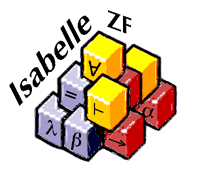
\includegraphics[scale=0.5]{isabelle_zf} \\[4ex] 
       Isabelle's Logics: FOL and ZF}

\author{{\em Lawrence C. Paulson}\\
        Computer Laboratory \\ University of Cambridge \\
        \texttt{lcp@cl.cam.ac.uk}\\[3ex] 
        With Contributions by Tobias Nipkow and Markus Wenzel%
\thanks{Markus Wenzel made numerous improvements.
    Philippe de Groote contributed to~\ZF{}.  Philippe No\"el and
    Martin Coen made many contributions to~\ZF{}.  The research has 
    been funded by the EPSRC (grants GR/G53279, GR/H40570, GR/K57381,
    GR/K77051) and by ESPRIT project 6453: Types.}
}

\newcommand\subcaption[1]{\par {\centering\normalsize\sc#1\par}\bigskip
  \hrule\bigskip}
\newenvironment{constants}{\begin{center}\small\begin{tabular}{rrrr}}{\end{tabular}\end{center}}

\makeindex

\underscoreoff

\setcounter{secnumdepth}{2} \setcounter{tocdepth}{2}  %% {secnumdepth}{2}???

\pagestyle{headings}
\sloppy
\binperiod     %%%treat . like a binary operator

\begin{document}
\maketitle 

\begin{abstract}
This manual describes Isabelle's formalizations of many-sorted first-order
logic (\texttt{FOL}) and Zermelo-Fraenkel set theory (\texttt{ZF}).  See the
\emph{Reference Manual} for general Isabelle commands, and \emph{Introduction
  to Isabelle} for an overall tutorial.
\end{abstract}

\pagenumbering{roman} \tableofcontents \clearfirst

\chapter{Syntax primitives}

The rather generic framework of Isabelle/Isar syntax emerges from three main
syntactic categories: \emph{commands} of the top-level Isar engine (covering
theory and proof elements), \emph{methods} for general goal refinements
(analogous to traditional ``tactics''), and \emph{attributes} for operations
on facts (within a certain context).  Here we give a reference of basic
syntactic entities underlying Isabelle/Isar syntax in a bottom-up manner.
Concrete theory and proof language elements will be introduced later on.

\medskip

In order to get started with writing well-formed Isabelle/Isar documents, the
most important aspect to be noted is the difference of \emph{inner} versus
\emph{outer} syntax.  Inner syntax is that of Isabelle types and terms of the
logic, while outer syntax is that of Isabelle/Isar theory sources (including
proofs).  As a general rule, inner syntax entities may occur only as
\emph{atomic entities} within outer syntax.  For example, the string
\texttt{"x + y"} and identifier \texttt{z} are legal term specifications
within a theory, while \texttt{x + y} is not.

\begin{warn}
  Old-style Isabelle theories used to fake parts of the inner syntax of types,
  with rather complicated rules when quotes may be omitted.  Despite the minor
  drawback of requiring quotes more often, the syntax of Isabelle/Isar is
  somewhat simpler and more robust in that respect.
\end{warn}

Printed theory documents usually omit quotes to gain readability (this is a
matter of {\LaTeX} macro setup, say via \verb,\isabellestyle,, see also
\cite{isabelle-sys}).  Experienced users of Isabelle/Isar may easily
reconstruct the lost technical information, while mere readers need not care
about quotes at all.

\medskip

Isabelle/Isar input may contain any number of input termination characters
``\texttt{;}'' (semicolon) to separate commands explicitly.  This is
particularly useful in interactive shell sessions to make clear where the
current command is intended to end.  Otherwise, the interpreter loop will
continue to issue a secondary prompt ``\verb,#,'' until an end-of-command is
clearly recognized from the input syntax, e.g.\ encounter of the next command
keyword.

Advanced interfaces such as Proof~General \cite{proofgeneral} do not require
explicit semicolons, the amount of input text is determined automatically by
inspecting the present content of the Emacs text buffer.  In the printed
presentation of Isabelle/Isar documents semicolons are omitted altogether for
readability.

\begin{warn}
  Proof~General requires certain syntax classification tables in order to
  achieve properly synchronized interaction with the Isabelle/Isar process.
  These tables need to be consistent with the Isabelle version and particular
  logic image to be used in a running session (common object-logics may well
  change the outer syntax).  The standard setup should work correctly with any
  of the ``official'' logic images derived from Isabelle/HOL (including HOLCF
  etc.).  Users of alternative logics may need to tell Proof~General
  explicitly, e.g.\ by giving an option \verb,-k ZF, (in conjunction with
  \verb,-l ZF, to specify the default logic image).
\end{warn}

\section{Lexical matters}\label{sec:lex-syntax}

The Isabelle/Isar outer syntax provides token classes as presented below; most
of these coincide with the inner lexical syntax as presented in
\cite{isabelle-ref}.

\indexoutertoken{ident}\indexoutertoken{longident}\indexoutertoken{symident}
\indexoutertoken{nat}\indexoutertoken{var}\indexoutertoken{typefree}
\indexoutertoken{typevar}\indexoutertoken{string}\indexoutertoken{verbatim}
\begin{matharray}{rcl}
  ident & = & letter\,quasiletter^* \\
  longident & = & ident (\verb,.,ident)^+ \\
  symident & = & sym^+ ~|~ \verb,\<,ident\verb,>, \\
  nat & = & digit^+ \\
  var & = & ident ~|~ \verb,?,ident ~|~ \verb,?,ident\verb,.,nat \\
  typefree & = & \verb,',ident \\
  typevar & = & typefree ~|~ \verb,?,typefree ~|~ \verb,?,typefree\verb,.,nat \\
  string & = & \verb,", ~\dots~ \verb,", \\
  verbatim & = & \verb,{*, ~\dots~ \verb,*}, \\[1ex]

  letter & = & latin ~|~ \verb,\<,latin\verb,>, ~|~ \verb,\<,latin\,latin\verb,>, ~|~ greek ~|~ \\
         &   & \verb,\<^isub>, ~|~ \verb,\<^isup>, \\
  quasiletter & = & letter ~|~ digit ~|~ \verb,_, ~|~ \verb,', \\
  latin & = & \verb,a, ~|~ \dots ~|~ \verb,z, ~|~ \verb,A, ~|~ \dots ~|~ \verb,Z, \\
  digit & = & \verb,0, ~|~ \dots ~|~ \verb,9, \\
  sym & = & \verb,!, ~|~ \verb,#, ~|~ \verb,$, ~|~ \verb,%, ~|~ \verb,&, ~|~  %$
   \verb,*, ~|~ \verb,+, ~|~ \verb,-, ~|~ \verb,/, ~|~ \verb,:, ~|~ \\
  & & \verb,<, ~|~ \verb,=, ~|~ \verb,>, ~|~ \verb,?, ~|~ \texttt{\at} ~|~
  \verb,^, ~|~ \verb,_, ~|~ \verb,`, ~|~ \verb,|, ~|~ \verb,~, \\
greek & = & \verb,\<alpha>, ~|~ \verb,\<beta>, ~|~ \verb,\<gamma>, ~|~ \verb,\<delta>, ~| \\
      &   & \verb,\<epsilon>, ~|~ \verb,\<zeta>, ~|~ \verb,\<eta>, ~|~ \verb,\<theta>, ~| \\
      &   & \verb,\<iota>, ~|~ \verb,\<kappa>, ~|~ \verb,\<mu>, ~|~ \verb,\<nu>, ~| \\
      &   & \verb,\<xi>, ~|~ \verb,\<pi>, ~|~ \verb,\<rho>, ~|~ \verb,\<sigma>, ~| \\
      &   & \verb,\<tau>, ~|~ \verb,\<upsilon>, ~|~ \verb,\<phi>, ~|~ \verb,\<psi>, ~| \\
      &   & \verb,\<omega>, ~|~ \verb,\<Gamma>, ~|~ \verb,\<Delta>, ~|~ \verb,\<Theta>, ~| \\
      &   & \verb,\<Lambda>, ~|~ \verb,\<Xi>, ~|~ \verb,\<Pi>, ~|~ \verb,\<Sigma>, ~| \\
      &   & \verb,\<Upsilon>, ~|~ \verb,\<Phi>, ~|~ \verb,\<Psi>, ~|~ \verb,\<Omega>, \\
\end{matharray}

The syntax of $string$ admits any characters, including newlines; ``\verb|"|''
(double-quote) and ``\verb|\|'' (backslash) need to be escaped by a backslash.
The body of $verbatim$ may consist of any text not containing ``\verb|*}|'';
this allows convenient inclusion of quotes without further escapes.  The greek
letters do \emph{not} include \verb,\<lambda>,, which is already used
differently in the meta-logic.

Common mathematical symbols such as $\forall$ are represented in Isabelle as
\verb,\<forall>,.  There are infinitely many legal symbols like this, although
proper presentation is left to front-end tools such as {\LaTeX} or
Proof~General with the X-Symbol package.  A list of standard Isabelle symbols
that work well with these tools is given in \cite[appendix~A]{isabelle-sys}.

Comments take the form \texttt{(*~\dots~*)} and may be nested, although
user-interface tools may prevent this.  Note that \texttt{(*~\dots~*)}
indicate source comments only, which are stripped after lexical analysis of
the input.  The Isar document syntax also provides formal comments that are
considered as part of the text (see \S\ref{sec:comments}).

\begin{warn}
  Proof~General does not handle nested comments properly; it is also unable to
  keep \verb,(*,\,/\,\verb,{*, and \verb,*),\,/\,\verb,*}, apart, despite
  their rather different meaning.  These are inherent problems of Emacs
  legacy.  Users should not be overly aggressive about nesting or alternating
  these delimiters.
\end{warn}


\section{Common syntax entities}

Subsequently, we introduce several basic syntactic entities, such as names,
terms, and theorem specifications, which have been factored out of the actual
Isar language elements to be described later.

Note that some of the basic syntactic entities introduced below (e.g.\
\railqtok{name}) act much like tokens rather than plain nonterminals (e.g.\
\railnonterm{sort}), especially for the sake of error messages.  E.g.\ syntax
elements like $\CONSTS$ referring to \railqtok{name} or \railqtok{type} would
really report a missing name or type rather than any of the constituent
primitive tokens such as \railtok{ident} or \railtok{string}.


\subsection{Names}

Entity \railqtok{name} usually refers to any name of types, constants,
theorems etc.\ that are to be \emph{declared} or \emph{defined} (so qualified
identifiers are excluded here).  Quoted strings provide an escape for
non-identifier names or those ruled out by outer syntax keywords (e.g.\
\verb|"let"|).  Already existing objects are usually referenced by
\railqtok{nameref}.

\indexoutertoken{name}\indexoutertoken{parname}\indexoutertoken{nameref}
\indexoutertoken{int}
\begin{rail}
  name: ident | symident | string | nat
  ;
  parname: '(' name ')'
  ;
  nameref: name | longident
  ;
  int: nat | '-' nat
  ;
\end{rail}


\subsection{Comments}\label{sec:comments}

Large chunks of plain \railqtok{text} are usually given \railtok{verbatim},
i.e.\ enclosed in \verb|{*|~\dots~\verb|*}|.  For convenience, any of the
smaller text units conforming to \railqtok{nameref} are admitted as well.  A
marginal \railnonterm{comment} is of the form \texttt{--} \railqtok{text}.
Any number of these may occur within Isabelle/Isar commands.

\indexoutertoken{text}\indexouternonterm{comment}
\begin{rail}
  text: verbatim | nameref
  ;
  comment: '--' text
  ;
\end{rail}


\subsection{Type classes, sorts and arities}

Classes are specified by plain names.  Sorts have a very simple inner syntax,
which is either a single class name $c$ or a list $\{c@1, \dots, c@n\}$
referring to the intersection of these classes.  The syntax of type arities is
given directly at the outer level.

\railalias{subseteq}{\isasymsubseteq}
\railterm{subseteq}

\indexouternonterm{sort}\indexouternonterm{arity}
\indexouternonterm{classdecl}
\begin{rail}
  classdecl: name (('<' | subseteq) (nameref + ','))?
  ;
  sort: nameref
  ;
  arity: ('(' (sort + ',') ')')? sort
  ;
\end{rail}


\subsection{Types and terms}\label{sec:types-terms}

The actual inner Isabelle syntax, that of types and terms of the logic, is far
too sophisticated in order to be modelled explicitly at the outer theory
level.  Basically, any such entity has to be quoted to turn it into a single
token (the parsing and type-checking is performed internally later).  For
convenience, a slightly more liberal convention is adopted: quotes may be
omitted for any type or term that is already atomic at the outer level.  For
example, one may just write \texttt{x} instead of \texttt{"x"}.  Note that
symbolic identifiers (e.g.\ \texttt{++} or $\forall$) are available as well,
provided these have not been superseded by commands or other keywords already
(e.g.\ \texttt{=} or \texttt{+}).

\indexoutertoken{type}\indexoutertoken{term}\indexoutertoken{prop}
\begin{rail}
  type: nameref | typefree | typevar
  ;
  term: nameref | var
  ;
  prop: term
  ;
\end{rail}

Positional instantiations are indicated by giving a sequence of terms, or the
placeholder ``$\_$'' (underscore), which means to skip a position.

\indexoutertoken{inst}\indexoutertoken{insts}
\begin{rail}
  inst: underscore | term
  ;
  insts: (inst *)
  ;
\end{rail}

Type declarations and definitions usually refer to \railnonterm{typespec} on
the left-hand side.  This models basic type constructor application at the
outer syntax level.  Note that only plain postfix notation is available here,
but no infixes.

\indexouternonterm{typespec}
\begin{rail}
  typespec: (() | typefree | '(' ( typefree + ',' ) ')') name
  ;
\end{rail}


\subsection{Mixfix annotations}

Mixfix annotations specify concrete \emph{inner} syntax of Isabelle types and
terms.  Some commands such as $\TYPES$ (see \S\ref{sec:types-pure}) admit
infixes only, while $\CONSTS$ (see \S\ref{sec:consts}) and
$\isarkeyword{syntax}$ (see \S\ref{sec:syn-trans}) support the full range of
general mixfixes and binders.

\indexouternonterm{infix}\indexouternonterm{mixfix}\indexouternonterm{structmixfix}
\begin{rail}
  infix: '(' ('infix' | 'infixl' | 'infixr') string? nat ')'
  ;
  mixfix: infix | '(' string prios? nat? ')' | '(' 'binder' string prios? nat ')'
  ;
  structmixfix: mixfix | '(' 'structure' ')'
  ;

  prios: '[' (nat + ',') ']'
  ;
\end{rail}

Here the \railtok{string} specifications refer to the actual mixfix template
(see also \cite{isabelle-ref}), which may include literal text, spacing,
blocks, and arguments (denoted by ``$_$''); the special symbol \verb,\<index>,
(printed as ``\i'') represents an index argument that specifies an implicit
structure reference (see also \S\ref{sec:locale}).  Infix and binder
declarations provide common abbreviations for particular mixfix declarations.
So in practice, mixfix templates mostly degenerate to literal text for
concrete syntax, such as ``\verb,++,'' for an infix symbol, or ``\verb,++,\i''
for an infix of an implicit structure.



\subsection{Proof methods}\label{sec:syn-meth}

Proof methods are either basic ones, or expressions composed of methods via
``\texttt{,}'' (sequential composition), ``\texttt{|}'' (alternative choices),
``\texttt{?}'' (try), ``\texttt{+}'' (repeat at least once).  In practice,
proof methods are usually just a comma separated list of
\railqtok{nameref}~\railnonterm{args} specifications.  Note that parentheses
may be dropped for single method specifications (with no arguments).

\indexouternonterm{method}
\begin{rail}
  method: (nameref | '(' methods ')') (() | '?' | '+')
  ;
  methods: (nameref args | method) + (',' | '|')
  ;
\end{rail}

Proper use of Isar proof methods does \emph{not} involve goal addressing.
Nevertheless, specifying goal ranges may occasionally come in handy in
emulating tactic scripts.  Note that $[n-]$ refers to all goals, starting from
$n$.  All goals may be specified by $[!]$, which is the same as $[1-]$.

\indexouternonterm{goalspec}
\begin{rail}
  goalspec: '[' (nat '-' nat | nat '-' | nat | '!' ) ']'
  ;
\end{rail}


\subsection{Attributes and theorems}\label{sec:syn-att}

Attributes (and proof methods, see \S\ref{sec:syn-meth}) have their own
``semi-inner'' syntax, in the sense that input conforming to
\railnonterm{args} below is parsed by the attribute a second time.  The
attribute argument specifications may be any sequence of atomic entities
(identifiers, strings etc.), or properly bracketed argument lists.  Below
\railqtok{atom} refers to any atomic entity, including any \railtok{keyword}
conforming to \railtok{symident}.

\indexoutertoken{atom}\indexouternonterm{args}\indexouternonterm{attributes}
\begin{rail}
  atom: nameref | typefree | typevar | var | nat | keyword
  ;
  arg: atom | '(' args ')' | '[' args ']'
  ;
  args: arg *
  ;
  attributes: '[' (nameref args * ',') ']'
  ;
\end{rail}

Theorem specifications come in several flavors: \railnonterm{axmdecl} and
\railnonterm{thmdecl} usually refer to axioms, assumptions or results of goal
statements, while \railnonterm{thmdef} collects lists of existing theorems.
Existing theorems are given by \railnonterm{thmref} and \railnonterm{thmrefs},
the former requires an actual singleton result.  An optional index selection
specifies the individual theorems to be picked out of a given fact list.  Any
kind of theorem specification may include lists of attributes both on the left
and right hand sides; attributes are applied to any immediately preceding
fact.  If names are omitted, the theorems are not stored within the theorem
database of the theory or proof context, but any given attributes are applied
nonetheless.

\indexouternonterm{axmdecl}\indexouternonterm{thmdecl}
\indexouternonterm{thmdef}\indexouternonterm{thmref}
\indexouternonterm{thmrefs}\indexouternonterm{selection}
\begin{rail}
  axmdecl: name attributes? ':'
  ;
  thmdecl: thmbind ':'
  ;
  thmdef: thmbind '='
  ;
  thmref: nameref selection? attributes?
  ;
  thmrefs: thmref +
  ;

  thmbind: name attributes | name | attributes
  ;
  selection: '(' ((nat | nat '-' nat?) + ',') ')'
  ;
\end{rail}


\subsection{Term patterns and declarations}\label{sec:term-decls}

Wherever explicit propositions (or term fragments) occur in a proof text,
casual binding of schematic term variables may be given specified via patterns
of the form ``$\ISS{p@1\;\dots}{p@n}$''.  There are separate versions
available for \railqtok{term}s and \railqtok{prop}s.  The latter provides a
$\CONCLNAME$ part with patterns referring the (atomic) conclusion of a rule.

\indexouternonterm{termpat}\indexouternonterm{proppat}
\begin{rail}
  termpat: '(' ('is' term +) ')'
  ;
  proppat: '(' (('is' prop +) | 'concl' ('is' prop +) | ('is' prop +) 'concl' ('is' prop +)) ')'
  ;
\end{rail}

Declarations of local variables $x :: \tau$ and logical propositions $a :
\phi$ represent different views on the same principle of introducing a local
scope.  In practice, one may usually omit the typing of $vars$ (due to
type-inference), and the naming of propositions (due to implicit references of
current facts).  In any case, Isar proof elements usually admit to introduce
multiple such items simultaneously.

\indexouternonterm{vars}\indexouternonterm{props}
\begin{rail}
  vars: (name+) ('::' type)?
  ;
  props: thmdecl? (prop proppat? +)
  ;
\end{rail}

The treatment of multiple declarations corresponds to the complementary focus
of $vars$ versus $props$: in ``$x@1~\dots~x@n :: \tau$'' the typing refers to
all variables, while in $a\colon \phi@1~\dots~\phi@n$ the naming refers to all
propositions collectively.  Isar language elements that refer to $vars$ or
$props$ typically admit separate typings or namings via another level of
iteration, with explicit $\AND$ separators; e.g.\ see $\FIXNAME$ and
$\ASSUMENAME$ in \S\ref{sec:proof-context}.


\subsection{Antiquotations}\label{sec:antiq}

\begin{matharray}{rcl@{\hspace*{2cm}}rcl}
  thm & : & \isarantiq & text & : & \isarantiq \\
  prop & : & \isarantiq & goals & : & \isarantiq \\
  term & : & \isarantiq & subgoals & : & \isarantiq \\
  const & : & \isarantiq & prf & : & \isarantiq \\
  typeof & : & \isarantiq & full_prf & : & \isarantiq \\
  typ & : & \isarantiq \\  
  thm_style & : & \isarantiq \\  
  term_style & : & \isarantiq \\  
\end{matharray}

The text body of formal comments (see also \S\ref{sec:comments}) may contain
antiquotations of logical entities, such as theorems, terms and types, which
are to be presented in the final output produced by the Isabelle document
preparation system (see also \S\ref{sec:document-prep}).

Thus embedding of
``\texttt{{\at}{\ttlbrace}term~[show_types]~"f(x)~=~a~+~x"{\ttrbrace}}''
within a text block would cause
\isa{(f{\isasymColon}'a~{\isasymRightarrow}~'a)~(x{\isasymColon}'a)~=~(a{\isasymColon}'a)~+~x}
to appear in the final {\LaTeX} document.  Also note that theorem
antiquotations may involve attributes as well.  For example,
\texttt{{\at}{\ttlbrace}thm~sym~[no_vars]{\ttrbrace}} would print the
statement where all schematic variables have been replaced by fixed ones,
which are easier to read.

\indexisarant{thm}\indexisarant{prop}\indexisarant{term}\indexisarant{const}
\indexisarant{typeof}\indexisarant{typ}\indexisarant{thm-style}
\indexisarant{term-style}\indexisarant{text}\indexisarant{goals}
\indexisarant{subgoals}\indexisarant{prf}\indexisarant{full-prf}

\begin{rail}
  atsign lbrace antiquotation rbrace
  ;

  antiquotation:
    'thm' options thmrefs |
    'prop' options prop |
    'term' options term |
    'const' options term |
    'typeof' options term |
    'typ' options type |
    'thm\_style' options style thmref |
    'term\_style' options style term |
    'text' options name |
    'goals' options |
    'subgoals' options |
    'prf' options thmrefs |
    'full\_prf' options thmrefs
  ;
  options: '[' (option * ',') ']'
  ;
  option: name | name '=' name
  ;
\end{rail}

Note that the syntax of antiquotations may \emph{not} include source comments
\texttt{(*~\dots~*)} or verbatim text \verb|{*|~\dots~\verb|*}|.

\begin{descr}

\item [$\at\{thm~\vec a\}$] prints theorems $\vec a$. Note that attribute
  specifications may be included as well (see also \S\ref{sec:syn-att}); the
  $no_vars$ operation (see \S\ref{sec:misc-meth-att}) would be particularly
  useful to suppress printing of schematic variables.

\item [$\at\{prop~\phi\}$] prints a well-typed proposition $\phi$.

\item [$\at\{term~t\}$] prints a well-typed term $t$.

\item [$\at\{const~c\}$] prints a well-defined constant $c$.

\item [$\at\{typeof~t\}$] prints the type of a well-typed term $t$.

\item [$\at\{typ~\tau\}$] prints a well-formed type $\tau$.

\item [$\at\{thm_style~s~a\}$] prints theorem $a$, previously
  applying a style $s$ to it; otherwise behaves the same as $\at\{thm~a\}$
  with just one theorem.

\item [$\at\{term_style~s~t\}$] prints a well-typed term $t$, previously
  applying a style $s$ to it; otherwise behaves the same as $\at\{term~t\}$.

\item [$\at\{text~s\}$] prints uninterpreted source text $s$.  This is
  particularly useful to print portions of text according to the Isabelle
  {\LaTeX} output style, without demanding well-formedness (e.g.\ small pieces
  of terms that should not be parsed or type-checked yet).

\item [$\at\{goals\}$] prints the current \emph{dynamic} goal state.  This is
  mainly for support of tactic-emulation scripts within Isar --- presentation
  of goal states does not conform to actual human-readable proof documents.
  Please do not include goal states into document output unless you really
  know what you are doing!

\item [$\at\{subgoals\}$] behaves almost like $goals$, except that it does not
  print the main goal.

\item [$\at\{prf~\vec a\}$] prints the (compact) proof terms corresponding to
  the theorems $\vec a$. Note that this
  requires proof terms to be switched on for the current object logic
  (see the ``Proof terms'' section of the Isabelle reference manual
  for information on how to do this).

\item [$\at\{full_prf~\vec a\}$] is like $\at\{prf~\vec a\}$, but displays
  the full proof terms, i.e.\ also displays information omitted in
  the compact proof term, which is denoted by ``$_$'' placeholders there.

\end{descr}

There are a few standard styles for use with $\at\{thm_style~s~a\}$ and
$\at\{term_style~s~t\}$:

\begin{descr}
  
\item [$lhs$] extracts the first argument of any application form with at
  least two arguments -- typically is meta-level or object-level equality or
  any other binary relation.
  
\item [$rhs$] similar to $lhs$, but extracts the second argument.
  
\item [$conlusion$] extracts the conclusion $C$ from nested meta-level
  implications $A@1 \Imp \cdots A@n \Imp C$.

\end{descr}

Further styles may be defined at ML level.

\medskip

The following options are available to tune the output.  Note that most of
these coincide with ML flags of the same names (see also \cite{isabelle-ref}).
\begin{descr}
\item[$show_types = bool$ and $show_sorts = bool$] control printing of
  explicit type and sort constraints.
\item[$show_structs = bool$] controls printing of implicit structures.
\item[$long_names = bool$] forces names of types and constants etc.\ to be
  printed in their fully qualified internal form.
\item[$eta_contract = bool$] prints terms in $\eta$-contracted form.
\item[$display = bool$] indicates if the text is to be output as multi-line
  ``display material'', rather than a small piece of text without line breaks
  (which is the default).
\item[$breaks = bool$] controls line breaks in non-display material.
\item[$quotes = bool$] indicates if the output should be enclosed in double
  quotes.
\item[$mode = name$] adds $name$ to the print mode to be used for presentation
  (see also \cite{isabelle-ref}).  Note that the standard setup for {\LaTeX}
  output is already present by default, including the modes ``$latex$'',
  ``$xsymbols$'', ``$symbols$''.
\item[$margin = nat$ and $indent = nat$] change the margin or indentation for
  pretty printing of display material.
\item[$source = bool$] prints the source text of the antiquotation arguments,
  rather than the actual value.  Note that this does not affect
  well-formedness checks of $thm$, $term$, etc. (only the $text$ antiquotation
  admits arbitrary output).
\item[$goals_limit = nat$] determines the maximum number of goals to be
  printed.
\item[$locale = name$] specifies an alternative context used for evaluating
  and printing the subsequent argument.
\end{descr}

For boolean flags, ``$name = true$'' may be abbreviated as ``$name$''.  All of
the above flags are disabled by default, unless changed from ML.

\medskip Note that antiquotations do not only spare the author from tedious
typing of logical entities, but also achieve some degree of
consistency-checking of informal explanations with formal developments:
well-formedness of terms and types with respect to the current theory or proof
context is ensured here.

%%% Local Variables:
%%% mode: latex
%%% TeX-master: "isar-ref"
%%% End:

%% $Id$
\chapter{First-Order Logic}
\index{first-order logic|(}

Isabelle implements Gentzen's natural deduction systems {\sc nj} and {\sc
  nk}.  Intuitionistic first-order logic is defined first, as theory
\thydx{IFOL}.  Classical logic, theory \thydx{FOL}, is
obtained by adding the double negation rule.  Basic proof procedures are
provided.  The intuitionistic prover works with derived rules to simplify
implications in the assumptions.  Classical~\texttt{FOL} employs Isabelle's
classical reasoner, which simulates a sequent calculus.

\section{Syntax and rules of inference}
The logic is many-sorted, using Isabelle's type classes.  The class of
first-order terms is called \cldx{term} and is a subclass of \texttt{logic}.
No types of individuals are provided, but extensions can define types such
as \texttt{nat::term} and type constructors such as \texttt{list::(term)term}
(see the examples directory, \texttt{FOL/ex}).  Below, the type variable
$\alpha$ ranges over class \texttt{term}; the equality symbol and quantifiers
are polymorphic (many-sorted).  The type of formulae is~\tydx{o}, which
belongs to class~\cldx{logic}.  Figure~\ref{fol-syntax} gives the syntax.
Note that $a$\verb|~=|$b$ is translated to $\neg(a=b)$.

Figure~\ref{fol-rules} shows the inference rules with their~\ML\ names.
Negation is defined in the usual way for intuitionistic logic; $\neg P$
abbreviates $P\imp\bot$.  The biconditional~($\bimp$) is defined through
$\conj$ and~$\imp$; introduction and elimination rules are derived for it.

The unique existence quantifier, $\exists!x.P(x)$, is defined in terms
of~$\exists$ and~$\forall$.  An Isabelle binder, it admits nested
quantifications.  For instance, $\exists!x\;y.P(x,y)$ abbreviates
$\exists!x. \exists!y.P(x,y)$; note that this does not mean that there
exists a unique pair $(x,y)$ satisfying~$P(x,y)$.

Some intuitionistic derived rules are shown in
Fig.\ts\ref{fol-int-derived}, again with their \ML\ names.  These include
rules for the defined symbols $\neg$, $\bimp$ and $\exists!$.  Natural
deduction typically involves a combination of forward and backward
reasoning, particularly with the destruction rules $(\conj E)$,
$({\imp}E)$, and~$(\forall E)$.  Isabelle's backward style handles these
rules badly, so sequent-style rules are derived to eliminate conjunctions,
implications, and universal quantifiers.  Used with elim-resolution,
\tdx{allE} eliminates a universal quantifier while \tdx{all_dupE}
re-inserts the quantified formula for later use.  The rules {\tt
conj_impE}, etc., support the intuitionistic proof procedure
(see~\S\ref{fol-int-prover}).

See the files \texttt{FOL/IFOL.thy}, \texttt{FOL/IFOL.ML} and
\texttt{FOL/intprover.ML} for complete listings of the rules and
derived rules.

\begin{figure} 
\begin{center}
\begin{tabular}{rrr} 
  \it name      &\it meta-type  & \it description \\ 
  \cdx{Trueprop}& $o\To prop$           & coercion to $prop$\\
  \cdx{Not}     & $o\To o$              & negation ($\neg$) \\
  \cdx{True}    & $o$                   & tautology ($\top$) \\
  \cdx{False}   & $o$                   & absurdity ($\bot$)
\end{tabular}
\end{center}
\subcaption{Constants}

\begin{center}
\begin{tabular}{llrrr} 
  \it symbol &\it name     &\it meta-type & \it priority & \it description \\
  \sdx{ALL}  & \cdx{All}  & $(\alpha\To o)\To o$ & 10 & 
        universal quantifier ($\forall$) \\
  \sdx{EX}   & \cdx{Ex}   & $(\alpha\To o)\To o$ & 10 & 
        existential quantifier ($\exists$) \\
  \texttt{EX!}  & \cdx{Ex1}  & $(\alpha\To o)\To o$ & 10 & 
        unique existence ($\exists!$)
\end{tabular}
\index{*"E"X"! symbol}
\end{center}
\subcaption{Binders} 

\begin{center}
\index{*"= symbol}
\index{&@{\tt\&} symbol}
\index{*"| symbol}
\index{*"-"-"> symbol}
\index{*"<"-"> symbol}
\begin{tabular}{rrrr} 
  \it symbol    & \it meta-type         & \it priority & \it description \\ 
  \tt =         & $[\alpha,\alpha]\To o$ & Left 50 & equality ($=$) \\
  \tt \&        & $[o,o]\To o$          & Right 35 & conjunction ($\conj$) \\
  \tt |         & $[o,o]\To o$          & Right 30 & disjunction ($\disj$) \\
  \tt -->       & $[o,o]\To o$          & Right 25 & implication ($\imp$) \\
  \tt <->       & $[o,o]\To o$          & Right 25 & biconditional ($\bimp$) 
\end{tabular}
\end{center}
\subcaption{Infixes}

\dquotes
\[\begin{array}{rcl}
 formula & = & \hbox{expression of type~$o$} \\
         & | & term " = " term \quad| \quad term " \ttilde= " term \\
         & | & "\ttilde\ " formula \\
         & | & formula " \& " formula \\
         & | & formula " | " formula \\
         & | & formula " --> " formula \\
         & | & formula " <-> " formula \\
         & | & "ALL~" id~id^* " . " formula \\
         & | & "EX~~" id~id^* " . " formula \\
         & | & "EX!~" id~id^* " . " formula
  \end{array}
\]
\subcaption{Grammar}
\caption{Syntax of \texttt{FOL}} \label{fol-syntax}
\end{figure}


\begin{figure} 
\begin{ttbox}
\tdx{refl}        a=a
\tdx{subst}       [| a=b;  P(a) |] ==> P(b)
\subcaption{Equality rules}

\tdx{conjI}       [| P;  Q |] ==> P&Q
\tdx{conjunct1}   P&Q ==> P
\tdx{conjunct2}   P&Q ==> Q

\tdx{disjI1}      P ==> P|Q
\tdx{disjI2}      Q ==> P|Q
\tdx{disjE}       [| P|Q;  P ==> R;  Q ==> R |] ==> R

\tdx{impI}        (P ==> Q) ==> P-->Q
\tdx{mp}          [| P-->Q;  P |] ==> Q

\tdx{FalseE}      False ==> P
\subcaption{Propositional rules}

\tdx{allI}        (!!x. P(x))  ==> (ALL x.P(x))
\tdx{spec}        (ALL x.P(x)) ==> P(x)

\tdx{exI}         P(x) ==> (EX x.P(x))
\tdx{exE}         [| EX x.P(x);  !!x. P(x) ==> R |] ==> R
\subcaption{Quantifier rules}

\tdx{True_def}    True        == False-->False
\tdx{not_def}     ~P          == P-->False
\tdx{iff_def}     P<->Q       == (P-->Q) & (Q-->P)
\tdx{ex1_def}     EX! x. P(x) == EX x. P(x) & (ALL y. P(y) --> y=x)
\subcaption{Definitions}
\end{ttbox}

\caption{Rules of intuitionistic logic} \label{fol-rules}
\end{figure}


\begin{figure} 
\begin{ttbox}
\tdx{sym}       a=b ==> b=a
\tdx{trans}     [| a=b;  b=c |] ==> a=c
\tdx{ssubst}    [| b=a;  P(a) |] ==> P(b)
\subcaption{Derived equality rules}

\tdx{TrueI}     True

\tdx{notI}      (P ==> False) ==> ~P
\tdx{notE}      [| ~P;  P |] ==> R

\tdx{iffI}      [| P ==> Q;  Q ==> P |] ==> P<->Q
\tdx{iffE}      [| P <-> Q;  [| P-->Q; Q-->P |] ==> R |] ==> R
\tdx{iffD1}     [| P <-> Q;  P |] ==> Q            
\tdx{iffD2}     [| P <-> Q;  Q |] ==> P

\tdx{ex1I}      [| P(a);  !!x. P(x) ==> x=a |]  ==>  EX! x. P(x)
\tdx{ex1E}      [| EX! x.P(x);  !!x.[| P(x);  ALL y. P(y) --> y=x |] ==> R 
          |] ==> R
\subcaption{Derived rules for \(\top\), \(\neg\), \(\bimp\) and \(\exists!\)}

\tdx{conjE}     [| P&Q;  [| P; Q |] ==> R |] ==> R
\tdx{impE}      [| P-->Q;  P;  Q ==> R |] ==> R
\tdx{allE}      [| ALL x.P(x);  P(x) ==> R |] ==> R
\tdx{all_dupE}  [| ALL x.P(x);  [| P(x); ALL x.P(x) |] ==> R |] ==> R
\subcaption{Sequent-style elimination rules}

\tdx{conj_impE} [| (P&Q)-->S;  P-->(Q-->S) ==> R |] ==> R
\tdx{disj_impE} [| (P|Q)-->S;  [| P-->S; Q-->S |] ==> R |] ==> R
\tdx{imp_impE}  [| (P-->Q)-->S;  [| P; Q-->S |] ==> Q;  S ==> R |] ==> R
\tdx{not_impE}  [| ~P --> S;  P ==> False;  S ==> R |] ==> R
\tdx{iff_impE}  [| (P<->Q)-->S; [| P; Q-->S |] ==> Q; [| Q; P-->S |] ==> P;
             S ==> R |] ==> R
\tdx{all_impE}  [| (ALL x.P(x))-->S;  !!x.P(x);  S ==> R |] ==> R
\tdx{ex_impE}   [| (EX x.P(x))-->S;  P(a)-->S ==> R |] ==> R
\end{ttbox}
\subcaption{Intuitionistic simplification of implication}
\caption{Derived rules for intuitionistic logic} \label{fol-int-derived}
\end{figure}


\section{Generic packages}
FOL instantiates most of Isabelle's generic packages.
\begin{itemize}
\item 
It instantiates the simplifier.  Both equality ($=$) and the biconditional
($\bimp$) may be used for rewriting.  Tactics such as \texttt{Asm_simp_tac} and
\texttt{Full_simp_tac} refer to the default simpset (\texttt{simpset()}), which works for
most purposes.  Named simplification sets include \ttindexbold{IFOL_ss},
for intuitionistic first-order logic, and \ttindexbold{FOL_ss},
for classical logic.  See the file
\texttt{FOL/simpdata.ML} for a complete listing of the simplification
rules%
\iflabelundefined{sec:setting-up-simp}{}%
        {, and \S\ref{sec:setting-up-simp} for discussion}.

\item 
It instantiates the classical reasoner.  See~\S\ref{fol-cla-prover}
for details. 

\item FOL provides the tactic \ttindex{hyp_subst_tac}, which substitutes for
  an equality throughout a subgoal and its hypotheses.  This tactic uses FOL's
  general substitution rule.
\end{itemize}

\begin{warn}\index{simplification!of conjunctions}%
  Reducing $a=b\conj P(a)$ to $a=b\conj P(b)$ is sometimes advantageous.  The
  left part of a conjunction helps in simplifying the right part.  This effect
  is not available by default: it can be slow.  It can be obtained by
  including \ttindex{conj_cong} in a simpset, \verb$addcongs [conj_cong]$.
\end{warn}


\section{Intuitionistic proof procedures} \label{fol-int-prover}
Implication elimination (the rules~\texttt{mp} and~\texttt{impE}) pose
difficulties for automated proof.  In intuitionistic logic, the assumption
$P\imp Q$ cannot be treated like $\neg P\disj Q$.  Given $P\imp Q$, we may
use~$Q$ provided we can prove~$P$; the proof of~$P$ may require repeated
use of $P\imp Q$.  If the proof of~$P$ fails then the whole branch of the
proof must be abandoned.  Thus intuitionistic propositional logic requires
backtracking.  

For an elementary example, consider the intuitionistic proof of $Q$ from
$P\imp Q$ and $(P\imp Q)\imp P$.  The implication $P\imp Q$ is needed
twice:
\[ \infer[({\imp}E)]{Q}{P\imp Q &
       \infer[({\imp}E)]{P}{(P\imp Q)\imp P & P\imp Q}} 
\]
The theorem prover for intuitionistic logic does not use~\texttt{impE}.\@
Instead, it simplifies implications using derived rules
(Fig.\ts\ref{fol-int-derived}).  It reduces the antecedents of implications
to atoms and then uses Modus Ponens: from $P\imp Q$ and~$P$ deduce~$Q$.
The rules \tdx{conj_impE} and \tdx{disj_impE} are 
straightforward: $(P\conj Q)\imp S$ is equivalent to $P\imp (Q\imp S)$, and
$(P\disj Q)\imp S$ is equivalent to the conjunction of $P\imp S$ and $Q\imp
S$.  The other \ldots{\tt_impE} rules are unsafe; the method requires
backtracking.  All the rules are derived in the same simple manner.

Dyckhoff has independently discovered similar rules, and (more importantly)
has demonstrated their completeness for propositional
logic~\cite{dyckhoff}.  However, the tactics given below are not complete
for first-order logic because they discard universally quantified
assumptions after a single use.
\begin{ttbox} 
mp_tac              : int -> tactic
eq_mp_tac           : int -> tactic
IntPr.safe_step_tac : int -> tactic
IntPr.safe_tac      :        tactic
IntPr.inst_step_tac : int -> tactic
IntPr.step_tac      : int -> tactic
IntPr.fast_tac      : int -> tactic
IntPr.best_tac      : int -> tactic
\end{ttbox}
Most of these belong to the structure \texttt{IntPr} and resemble the
tactics of Isabelle's classical reasoner.

\begin{ttdescription}
\item[\ttindexbold{mp_tac} {\it i}] 
attempts to use \tdx{notE} or \tdx{impE} within the assumptions in
subgoal $i$.  For each assumption of the form $\neg P$ or $P\imp Q$, it
searches for another assumption unifiable with~$P$.  By
contradiction with $\neg P$ it can solve the subgoal completely; by Modus
Ponens it can replace the assumption $P\imp Q$ by $Q$.  The tactic can
produce multiple outcomes, enumerating all suitable pairs of assumptions.

\item[\ttindexbold{eq_mp_tac} {\it i}] 
is like \texttt{mp_tac} {\it i}, but may not instantiate unknowns --- thus, it
is safe.

\item[\ttindexbold{IntPr.safe_step_tac} $i$] performs a safe step on
subgoal~$i$.  This may include proof by assumption or Modus Ponens (taking
care not to instantiate unknowns), or \texttt{hyp_subst_tac}. 

\item[\ttindexbold{IntPr.safe_tac}] repeatedly performs safe steps on all 
subgoals.  It is deterministic, with at most one outcome.

\item[\ttindexbold{IntPr.inst_step_tac} $i$] is like \texttt{safe_step_tac},
but allows unknowns to be instantiated.

\item[\ttindexbold{IntPr.step_tac} $i$] tries \texttt{safe_tac} or {\tt
    inst_step_tac}, or applies an unsafe rule.  This is the basic step of
  the intuitionistic proof procedure.

\item[\ttindexbold{IntPr.fast_tac} $i$] applies \texttt{step_tac}, using
depth-first search, to solve subgoal~$i$.

\item[\ttindexbold{IntPr.best_tac} $i$] applies \texttt{step_tac}, using
best-first search (guided by the size of the proof state) to solve subgoal~$i$.
\end{ttdescription}
Here are some of the theorems that \texttt{IntPr.fast_tac} proves
automatically.  The latter three date from {\it Principia Mathematica}
(*11.53, *11.55, *11.61)~\cite{principia}.
\begin{ttbox}
~~P & ~~(P --> Q) --> ~~Q
(ALL x y. P(x) --> Q(y)) <-> ((EX x. P(x)) --> (ALL y. Q(y)))
(EX x y. P(x) & Q(x,y)) <-> (EX x. P(x) & (EX y. Q(x,y)))
(EX y. ALL x. P(x) --> Q(x,y)) --> (ALL x. P(x) --> (EX y. Q(x,y)))
\end{ttbox}



\begin{figure} 
\begin{ttbox}
\tdx{excluded_middle}    ~P | P

\tdx{disjCI}    (~Q ==> P) ==> P|Q
\tdx{exCI}      (ALL x. ~P(x) ==> P(a)) ==> EX x.P(x)
\tdx{impCE}     [| P-->Q; ~P ==> R; Q ==> R |] ==> R
\tdx{iffCE}     [| P<->Q;  [| P; Q |] ==> R;  [| ~P; ~Q |] ==> R |] ==> R
\tdx{notnotD}   ~~P ==> P
\tdx{swap}      ~P ==> (~Q ==> P) ==> Q
\end{ttbox}
\caption{Derived rules for classical logic} \label{fol-cla-derived}
\end{figure}


\section{Classical proof procedures} \label{fol-cla-prover}
The classical theory, \thydx{FOL}, consists of intuitionistic logic plus
the rule
$$ \vcenter{\infer{P}{\infer*{P}{[\neg P]}}} \eqno(classical) $$
\noindent
Natural deduction in classical logic is not really all that natural.  FOL
derives classical introduction rules for $\disj$ and~$\exists$, as well as
classical elimination rules for~$\imp$ and~$\bimp$, and the swap rule (see
Fig.\ts\ref{fol-cla-derived}).

The classical reasoner is installed.  Tactics such as \texttt{Blast_tac} and {\tt
Best_tac} refer to the default claset (\texttt{claset()}), which works for most
purposes.  Named clasets include \ttindexbold{prop_cs}, which includes the
propositional rules, and \ttindexbold{FOL_cs}, which also includes quantifier
rules.  See the file \texttt{FOL/cladata.ML} for lists of the
classical rules, and 
\iflabelundefined{chap:classical}{the {\em Reference Manual\/}}%
        {Chap.\ts\ref{chap:classical}} 
for more discussion of classical proof methods.


\section{An intuitionistic example}
Here is a session similar to one in {\em Logic and Computation}
\cite[pages~222--3]{paulson87}.  Isabelle treats quantifiers differently
from {\sc lcf}-based theorem provers such as {\sc hol}.  

First, we specify that we are working in intuitionistic logic:
\begin{ttbox}
context IFOL.thy;
\end{ttbox}
The proof begins by entering the goal, then applying the rule $({\imp}I)$.
\begin{ttbox}
Goal "(EX y. ALL x. Q(x,y)) -->  (ALL x. EX y. Q(x,y))";
{\out Level 0}
{\out (EX y. ALL x. Q(x,y)) --> (ALL x. EX y. Q(x,y))}
{\out  1. (EX y. ALL x. Q(x,y)) --> (ALL x. EX y. Q(x,y))}
\ttbreak
by (resolve_tac [impI] 1);
{\out Level 1}
{\out (EX y. ALL x. Q(x,y)) --> (ALL x. EX y. Q(x,y))}
{\out  1. EX y. ALL x. Q(x,y) ==> ALL x. EX y. Q(x,y)}
\end{ttbox}
In this example, we shall never have more than one subgoal.  Applying
$({\imp}I)$ replaces~\verb|-->| by~\verb|==>|, making
\(\ex{y}\all{x}Q(x,y)\) an assumption.  We have the choice of
$({\exists}E)$ and $({\forall}I)$; let us try the latter.
\begin{ttbox}
by (resolve_tac [allI] 1);
{\out Level 2}
{\out (EX y. ALL x. Q(x,y)) --> (ALL x. EX y. Q(x,y))}
{\out  1. !!x. EX y. ALL x. Q(x,y) ==> EX y. Q(x,y)}
\end{ttbox}
Applying $({\forall}I)$ replaces the \texttt{ALL~x} by \hbox{\tt!!x},
changing the universal quantifier from object~($\forall$) to
meta~($\Forall$).  The bound variable is a {\bf parameter} of the
subgoal.  We now must choose between $({\exists}I)$ and $({\exists}E)$.  What
happens if the wrong rule is chosen?
\begin{ttbox}
by (resolve_tac [exI] 1);
{\out Level 3}
{\out (EX y. ALL x. Q(x,y)) --> (ALL x. EX y. Q(x,y))}
{\out  1. !!x. EX y. ALL x. Q(x,y) ==> Q(x,?y2(x))}
\end{ttbox}
The new subgoal~1 contains the function variable {\tt?y2}.  Instantiating
{\tt?y2} can replace~{\tt?y2(x)} by a term containing~\texttt{x}, even
though~\texttt{x} is a bound variable.  Now we analyse the assumption
\(\exists y.\forall x. Q(x,y)\) using elimination rules:
\begin{ttbox}
by (eresolve_tac [exE] 1);
{\out Level 4}
{\out (EX y. ALL x. Q(x,y)) --> (ALL x. EX y. Q(x,y))}
{\out  1. !!x y. ALL x. Q(x,y) ==> Q(x,?y2(x))}
\end{ttbox}
Applying $(\exists E)$ has produced the parameter \texttt{y} and stripped the
existential quantifier from the assumption.  But the subgoal is unprovable:
there is no way to unify \texttt{?y2(x)} with the bound variable~\texttt{y}.
Using \texttt{choplev} we can return to the critical point.  This time we
apply $({\exists}E)$:
\begin{ttbox}
choplev 2;
{\out Level 2}
{\out (EX y. ALL x. Q(x,y)) --> (ALL x. EX y. Q(x,y))}
{\out  1. !!x. EX y. ALL x. Q(x,y) ==> EX y. Q(x,y)}
\ttbreak
by (eresolve_tac [exE] 1);
{\out Level 3}
{\out (EX y. ALL x. Q(x,y)) --> (ALL x. EX y. Q(x,y))}
{\out  1. !!x y. ALL x. Q(x,y) ==> EX y. Q(x,y)}
\end{ttbox}
We now have two parameters and no scheme variables.  Applying
$({\exists}I)$ and $({\forall}E)$ produces two scheme variables, which are
applied to those parameters.  Parameters should be produced early, as this
example demonstrates.
\begin{ttbox}
by (resolve_tac [exI] 1);
{\out Level 4}
{\out (EX y. ALL x. Q(x,y)) --> (ALL x. EX y. Q(x,y))}
{\out  1. !!x y. ALL x. Q(x,y) ==> Q(x,?y3(x,y))}
\ttbreak
by (eresolve_tac [allE] 1);
{\out Level 5}
{\out (EX y. ALL x. Q(x,y)) --> (ALL x. EX y. Q(x,y))}
{\out  1. !!x y. Q(?x4(x,y),y) ==> Q(x,?y3(x,y))}
\end{ttbox}
The subgoal has variables \texttt{?y3} and \texttt{?x4} applied to both
parameters.  The obvious projection functions unify {\tt?x4(x,y)} with~{\tt
x} and \verb|?y3(x,y)| with~\texttt{y}.
\begin{ttbox}
by (assume_tac 1);
{\out Level 6}
{\out (EX y. ALL x. Q(x,y)) --> (ALL x. EX y. Q(x,y))}
{\out No subgoals!}
\end{ttbox}
The theorem was proved in six tactic steps, not counting the abandoned
ones.  But proof checking is tedious; \ttindex{IntPr.fast_tac} proves the
theorem in one step.
\begin{ttbox}
Goal "(EX y. ALL x. Q(x,y)) -->  (ALL x. EX y. Q(x,y))";
{\out Level 0}
{\out (EX y. ALL x. Q(x,y)) --> (ALL x. EX y. Q(x,y))}
{\out  1. (EX y. ALL x. Q(x,y)) --> (ALL x. EX y. Q(x,y))}
by (IntPr.fast_tac 1);
{\out Level 1}
{\out (EX y. ALL x. Q(x,y)) --> (ALL x. EX y. Q(x,y))}
{\out No subgoals!}
\end{ttbox}


\section{An example of intuitionistic negation}
The following example demonstrates the specialized forms of implication
elimination.  Even propositional formulae can be difficult to prove from
the basic rules; the specialized rules help considerably.  

Propositional examples are easy to invent.  As Dummett notes~\cite[page
28]{dummett}, $\neg P$ is classically provable if and only if it is
intuitionistically provable;  therefore, $P$ is classically provable if and
only if $\neg\neg P$ is intuitionistically provable.%
\footnote{Of course this holds only for propositional logic, not if $P$ is
  allowed to contain quantifiers.} Proving $\neg\neg P$ intuitionistically is
much harder than proving~$P$ classically.

Our example is the double negation of the classical tautology $(P\imp
Q)\disj (Q\imp P)$.  When stating the goal, we command Isabelle to expand
negations to implications using the definition $\neg P\equiv P\imp\bot$.
This allows use of the special implication rules.
\begin{ttbox}
Goalw [not_def] "~ ~ ((P-->Q) | (Q-->P))";
{\out Level 0}
{\out ~ ~ ((P --> Q) | (Q --> P))}
{\out  1. ((P --> Q) | (Q --> P) --> False) --> False}
\end{ttbox}
The first step is trivial.
\begin{ttbox}
by (resolve_tac [impI] 1);
{\out Level 1}
{\out ~ ~ ((P --> Q) | (Q --> P))}
{\out  1. (P --> Q) | (Q --> P) --> False ==> False}
\end{ttbox}
By $(\imp E)$ it would suffice to prove $(P\imp Q)\disj (Q\imp P)$, but
that formula is not a theorem of intuitionistic logic.  Instead we apply
the specialized implication rule \tdx{disj_impE}.  It splits the
assumption into two assumptions, one for each disjunct.
\begin{ttbox}
by (eresolve_tac [disj_impE] 1);
{\out Level 2}
{\out ~ ~ ((P --> Q) | (Q --> P))}
{\out  1. [| (P --> Q) --> False; (Q --> P) --> False |] ==> False}
\end{ttbox}
We cannot hope to prove $P\imp Q$ or $Q\imp P$ separately, but
their negations are inconsistent.  Applying \tdx{imp_impE} breaks down
the assumption $\neg(P\imp Q)$, asking to show~$Q$ while providing new
assumptions~$P$ and~$\neg Q$.
\begin{ttbox}
by (eresolve_tac [imp_impE] 1);
{\out Level 3}
{\out ~ ~ ((P --> Q) | (Q --> P))}
{\out  1. [| (Q --> P) --> False; P; Q --> False |] ==> Q}
{\out  2. [| (Q --> P) --> False; False |] ==> False}
\end{ttbox}
Subgoal~2 holds trivially; let us ignore it and continue working on
subgoal~1.  Thanks to the assumption~$P$, we could prove $Q\imp P$;
applying \tdx{imp_impE} is simpler.
\begin{ttbox}
by (eresolve_tac [imp_impE] 1);
{\out Level 4}
{\out ~ ~ ((P --> Q) | (Q --> P))}
{\out  1. [| P; Q --> False; Q; P --> False |] ==> P}
{\out  2. [| P; Q --> False; False |] ==> Q}
{\out  3. [| (Q --> P) --> False; False |] ==> False}
\end{ttbox}
The three subgoals are all trivial.
\begin{ttbox}
by (REPEAT (eresolve_tac [FalseE] 2));
{\out Level 5}
{\out ~ ~ ((P --> Q) | (Q --> P))}
{\out  1. [| P; Q --> False; Q; P --> False |] ==> P}
\ttbreak
by (assume_tac 1);
{\out Level 6}
{\out ~ ~ ((P --> Q) | (Q --> P))}
{\out No subgoals!}
\end{ttbox}
This proof is also trivial for \texttt{IntPr.fast_tac}.


\section{A classical example} \label{fol-cla-example}
To illustrate classical logic, we shall prove the theorem
$\ex{y}\all{x}P(y)\imp P(x)$.  Informally, the theorem can be proved as
follows.  Choose~$y$ such that~$\neg P(y)$, if such exists; otherwise
$\all{x}P(x)$ is true.  Either way the theorem holds.  First, we switch to
classical logic:
\begin{ttbox}
context FOL.thy;
\end{ttbox}

The formal proof does not conform in any obvious way to the sketch given
above.  The key inference is the first one, \tdx{exCI}; this classical
version of~$(\exists I)$ allows multiple instantiation of the quantifier.
\begin{ttbox}
Goal "EX y. ALL x. P(y)-->P(x)";
{\out Level 0}
{\out EX y. ALL x. P(y) --> P(x)}
{\out  1. EX y. ALL x. P(y) --> P(x)}
\ttbreak
by (resolve_tac [exCI] 1);
{\out Level 1}
{\out EX y. ALL x. P(y) --> P(x)}
{\out  1. ALL y. ~ (ALL x. P(y) --> P(x)) ==> ALL x. P(?a) --> P(x)}
\end{ttbox}
We can either exhibit a term {\tt?a} to satisfy the conclusion of
subgoal~1, or produce a contradiction from the assumption.  The next
steps are routine.
\begin{ttbox}
by (resolve_tac [allI] 1);
{\out Level 2}
{\out EX y. ALL x. P(y) --> P(x)}
{\out  1. !!x. ALL y. ~ (ALL x. P(y) --> P(x)) ==> P(?a) --> P(x)}
\ttbreak
by (resolve_tac [impI] 1);
{\out Level 3}
{\out EX y. ALL x. P(y) --> P(x)}
{\out  1. !!x. [| ALL y. ~ (ALL x. P(y) --> P(x)); P(?a) |] ==> P(x)}
\end{ttbox}
By the duality between $\exists$ and~$\forall$, applying~$(\forall E)$
in effect applies~$(\exists I)$ again.
\begin{ttbox}
by (eresolve_tac [allE] 1);
{\out Level 4}
{\out EX y. ALL x. P(y) --> P(x)}
{\out  1. !!x. [| P(?a); ~ (ALL xa. P(?y3(x)) --> P(xa)) |] ==> P(x)}
\end{ttbox}
In classical logic, a negated assumption is equivalent to a conclusion.  To
get this effect, we create a swapped version of $(\forall I)$ and apply it
using \ttindex{eresolve_tac}; we could equivalently have applied $(\forall
I)$ using \ttindex{swap_res_tac}.
\begin{ttbox}
allI RSN (2,swap);
{\out val it = "[| ~(ALL x. ?P1(x)); !!x. ~ ?Q ==> ?P1(x) |] ==> ?Q" : thm}
by (eresolve_tac [it] 1);
{\out Level 5}
{\out EX y. ALL x. P(y) --> P(x)}
{\out  1. !!x xa. [| P(?a); ~ P(x) |] ==> P(?y3(x)) --> P(xa)}
\end{ttbox}
The previous conclusion, \texttt{P(x)}, has become a negated assumption.
\begin{ttbox}
by (resolve_tac [impI] 1);
{\out Level 6}
{\out EX y. ALL x. P(y) --> P(x)}
{\out  1. !!x xa. [| P(?a); ~ P(x); P(?y3(x)) |] ==> P(xa)}
\end{ttbox}
The subgoal has three assumptions.  We produce a contradiction between the
\index{assumptions!contradictory} assumptions~\verb|~P(x)| and~{\tt
  P(?y3(x))}.  The proof never instantiates the unknown~{\tt?a}.
\begin{ttbox}
by (eresolve_tac [notE] 1);
{\out Level 7}
{\out EX y. ALL x. P(y) --> P(x)}
{\out  1. !!x xa. [| P(?a); P(?y3(x)) |] ==> P(x)}
\ttbreak
by (assume_tac 1);
{\out Level 8}
{\out EX y. ALL x. P(y) --> P(x)}
{\out No subgoals!}
\end{ttbox}
The civilised way to prove this theorem is through \ttindex{Blast_tac},
which automatically uses the classical version of~$(\exists I)$:
\begin{ttbox}
Goal "EX y. ALL x. P(y)-->P(x)";
{\out Level 0}
{\out EX y. ALL x. P(y) --> P(x)}
{\out  1. EX y. ALL x. P(y) --> P(x)}
by (Blast_tac 1);
{\out Depth = 0}
{\out Depth = 1}
{\out Depth = 2}
{\out Level 1}
{\out EX y. ALL x. P(y) --> P(x)}
{\out No subgoals!}
\end{ttbox}
If this theorem seems counterintuitive, then perhaps you are an
intuitionist.  In constructive logic, proving $\ex{y}\all{x}P(y)\imp P(x)$
requires exhibiting a particular term~$t$ such that $\all{x}P(t)\imp P(x)$,
which we cannot do without further knowledge about~$P$.


\section{Derived rules and the classical tactics}
Classical first-order logic can be extended with the propositional
connective $if(P,Q,R)$, where 
$$ if(P,Q,R) \equiv P\conj Q \disj \neg P \conj R. \eqno(if) $$
Theorems about $if$ can be proved by treating this as an abbreviation,
replacing $if(P,Q,R)$ by $P\conj Q \disj \neg P \conj R$ in subgoals.  But
this duplicates~$P$, causing an exponential blowup and an unreadable
formula.  Introducing further abbreviations makes the problem worse.

Natural deduction demands rules that introduce and eliminate $if(P,Q,R)$
directly, without reference to its definition.  The simple identity
\[ if(P,Q,R) \,\bimp\, (P\imp Q)\conj (\neg P\imp R) \]
suggests that the
$if$-introduction rule should be
\[ \infer[({if}\,I)]{if(P,Q,R)}{\infer*{Q}{[P]}  &  \infer*{R}{[\neg P]}} \]
The $if$-elimination rule reflects the definition of $if(P,Q,R)$ and the
elimination rules for~$\disj$ and~$\conj$.
\[ \infer[({if}\,E)]{S}{if(P,Q,R) & \infer*{S}{[P,Q]}
                                  & \infer*{S}{[\neg P,R]}} 
\]
Having made these plans, we get down to work with Isabelle.  The theory of
classical logic, \texttt{FOL}, is extended with the constant
$if::[o,o,o]\To o$.  The axiom \tdx{if_def} asserts the
equation~$(if)$.
\begin{ttbox}
If = FOL +
consts  if     :: [o,o,o]=>o
rules   if_def "if(P,Q,R) == P&Q | ~P&R"
end
\end{ttbox}
We create the file \texttt{If.thy} containing these declarations.  (This file
is on directory \texttt{FOL/ex} in the Isabelle distribution.)  Typing
\begin{ttbox}
use_thy "If";  
\end{ttbox}
loads that theory and sets it to be the current context.


\subsection{Deriving the introduction rule}

The derivations of the introduction and elimination rules demonstrate the
methods for rewriting with definitions.  Classical reasoning is required,
so we use \texttt{blast_tac}.

The introduction rule, given the premises $P\Imp Q$ and $\neg P\Imp R$,
concludes $if(P,Q,R)$.  We propose the conclusion as the main goal
using~\ttindex{Goalw}, which uses \texttt{if_def} to rewrite occurrences
of $if$ in the subgoal.
\begin{ttbox}
val prems = Goalw [if_def]
    "[| P ==> Q; ~ P ==> R |] ==> if(P,Q,R)";
{\out Level 0}
{\out if(P,Q,R)}
{\out  1. P & Q | ~ P & R}
\end{ttbox}
The premises (bound to the {\ML} variable \texttt{prems}) are passed as
introduction rules to \ttindex{blast_tac}.  Remember that \texttt{claset()} refers
to the default classical set.
\begin{ttbox}
by (blast_tac (claset() addIs prems) 1);
{\out Level 1}
{\out if(P,Q,R)}
{\out No subgoals!}
qed "ifI";
\end{ttbox}


\subsection{Deriving the elimination rule}
The elimination rule has three premises, two of which are themselves rules.
The conclusion is simply $S$.
\begin{ttbox}
val major::prems = Goalw [if_def]
   "[| if(P,Q,R);  [| P; Q |] ==> S; [| ~ P; R |] ==> S |] ==> S";
{\out Level 0}
{\out S}
{\out  1. S}
\end{ttbox}
The major premise contains an occurrence of~$if$, but the version returned
by \ttindex{Goalw} (and bound to the {\ML} variable~\texttt{major}) has the
definition expanded.  Now \ttindex{cut_facts_tac} inserts~\texttt{major} as an
assumption in the subgoal, so that \ttindex{blast_tac} can break it down.
\begin{ttbox}
by (cut_facts_tac [major] 1);
{\out Level 1}
{\out S}
{\out  1. P & Q | ~ P & R ==> S}
\ttbreak
by (blast_tac (claset() addIs prems) 1);
{\out Level 2}
{\out S}
{\out No subgoals!}
qed "ifE";
\end{ttbox}
As you may recall from
\iflabelundefined{definitions}{{\em Introduction to Isabelle}}%
        {\S\ref{definitions}}, there are other
ways of treating definitions when deriving a rule.  We can start the
proof using \texttt{Goal}, which does not expand definitions, instead of
\texttt{Goalw}.  We can use \ttindex{rew_tac}
to expand definitions in the subgoals---perhaps after calling
\ttindex{cut_facts_tac} to insert the rule's premises.  We can use
\ttindex{rewrite_rule}, which is a meta-inference rule, to expand
definitions in the premises directly.


\subsection{Using the derived rules}
The rules just derived have been saved with the {\ML} names \tdx{ifI}
and~\tdx{ifE}.  They permit natural proofs of theorems such as the
following:
\begin{eqnarray*}
    if(P, if(Q,A,B), if(Q,C,D)) & \bimp & if(Q,if(P,A,C),if(P,B,D)) \\
    if(if(P,Q,R), A, B)         & \bimp & if(P,if(Q,A,B),if(R,A,B))
\end{eqnarray*}
Proofs also require the classical reasoning rules and the $\bimp$
introduction rule (called~\tdx{iffI}: do not confuse with~\texttt{ifI}). 

To display the $if$-rules in action, let us analyse a proof step by step.
\begin{ttbox}
Goal "if(P, if(Q,A,B), if(Q,C,D)) <-> if(Q, if(P,A,C), if(P,B,D))";
{\out Level 0}
{\out if(P,if(Q,A,B),if(Q,C,D)) <-> if(Q,if(P,A,C),if(P,B,D))}
{\out  1. if(P,if(Q,A,B),if(Q,C,D)) <-> if(Q,if(P,A,C),if(P,B,D))}
\ttbreak
by (resolve_tac [iffI] 1);
{\out Level 1}
{\out if(P,if(Q,A,B),if(Q,C,D)) <-> if(Q,if(P,A,C),if(P,B,D))}
{\out  1. if(P,if(Q,A,B),if(Q,C,D)) ==> if(Q,if(P,A,C),if(P,B,D))}
{\out  2. if(Q,if(P,A,C),if(P,B,D)) ==> if(P,if(Q,A,B),if(Q,C,D))}
\end{ttbox}
The $if$-elimination rule can be applied twice in succession.
\begin{ttbox}
by (eresolve_tac [ifE] 1);
{\out Level 2}
{\out if(P,if(Q,A,B),if(Q,C,D)) <-> if(Q,if(P,A,C),if(P,B,D))}
{\out  1. [| P; if(Q,A,B) |] ==> if(Q,if(P,A,C),if(P,B,D))}
{\out  2. [| ~ P; if(Q,C,D) |] ==> if(Q,if(P,A,C),if(P,B,D))}
{\out  3. if(Q,if(P,A,C),if(P,B,D)) ==> if(P,if(Q,A,B),if(Q,C,D))}
\ttbreak
by (eresolve_tac [ifE] 1);
{\out Level 3}
{\out if(P,if(Q,A,B),if(Q,C,D)) <-> if(Q,if(P,A,C),if(P,B,D))}
{\out  1. [| P; Q; A |] ==> if(Q,if(P,A,C),if(P,B,D))}
{\out  2. [| P; ~ Q; B |] ==> if(Q,if(P,A,C),if(P,B,D))}
{\out  3. [| ~ P; if(Q,C,D) |] ==> if(Q,if(P,A,C),if(P,B,D))}
{\out  4. if(Q,if(P,A,C),if(P,B,D)) ==> if(P,if(Q,A,B),if(Q,C,D))}
\end{ttbox}
%
In the first two subgoals, all assumptions have been reduced to atoms.  Now
$if$-introduction can be applied.  Observe how the $if$-rules break down
occurrences of $if$ when they become the outermost connective.
\begin{ttbox}
by (resolve_tac [ifI] 1);
{\out Level 4}
{\out if(P,if(Q,A,B),if(Q,C,D)) <-> if(Q,if(P,A,C),if(P,B,D))}
{\out  1. [| P; Q; A; Q |] ==> if(P,A,C)}
{\out  2. [| P; Q; A; ~ Q |] ==> if(P,B,D)}
{\out  3. [| P; ~ Q; B |] ==> if(Q,if(P,A,C),if(P,B,D))}
{\out  4. [| ~ P; if(Q,C,D) |] ==> if(Q,if(P,A,C),if(P,B,D))}
{\out  5. if(Q,if(P,A,C),if(P,B,D)) ==> if(P,if(Q,A,B),if(Q,C,D))}
\ttbreak
by (resolve_tac [ifI] 1);
{\out Level 5}
{\out if(P,if(Q,A,B),if(Q,C,D)) <-> if(Q,if(P,A,C),if(P,B,D))}
{\out  1. [| P; Q; A; Q; P |] ==> A}
{\out  2. [| P; Q; A; Q; ~ P |] ==> C}
{\out  3. [| P; Q; A; ~ Q |] ==> if(P,B,D)}
{\out  4. [| P; ~ Q; B |] ==> if(Q,if(P,A,C),if(P,B,D))}
{\out  5. [| ~ P; if(Q,C,D) |] ==> if(Q,if(P,A,C),if(P,B,D))}
{\out  6. if(Q,if(P,A,C),if(P,B,D)) ==> if(P,if(Q,A,B),if(Q,C,D))}
\end{ttbox}
Where do we stand?  The first subgoal holds by assumption; the second and
third, by contradiction.  This is getting tedious.  We could use the classical
reasoner, but first let us extend the default claset with the derived rules
for~$if$.
\begin{ttbox}
AddSIs [ifI];
AddSEs [ifE];
\end{ttbox}
Now we can revert to the
initial proof state and let \ttindex{blast_tac} solve it.  
\begin{ttbox}
choplev 0;
{\out Level 0}
{\out if(P,if(Q,A,B),if(Q,C,D)) <-> if(Q,if(P,A,C),if(P,B,D))}
{\out  1. if(P,if(Q,A,B),if(Q,C,D)) <-> if(Q,if(P,A,C),if(P,B,D))}
by (Blast_tac 1);
{\out Level 1}
{\out if(P,if(Q,A,B),if(Q,C,D)) <-> if(Q,if(P,A,C),if(P,B,D))}
{\out No subgoals!}
\end{ttbox}
This tactic also solves the other example.
\begin{ttbox}
Goal "if(if(P,Q,R), A, B) <-> if(P, if(Q,A,B), if(R,A,B))";
{\out Level 0}
{\out if(if(P,Q,R),A,B) <-> if(P,if(Q,A,B),if(R,A,B))}
{\out  1. if(if(P,Q,R),A,B) <-> if(P,if(Q,A,B),if(R,A,B))}
\ttbreak
by (Blast_tac 1);
{\out Level 1}
{\out if(if(P,Q,R),A,B) <-> if(P,if(Q,A,B),if(R,A,B))}
{\out No subgoals!}
\end{ttbox}


\subsection{Derived rules versus definitions}
Dispensing with the derived rules, we can treat $if$ as an
abbreviation, and let \ttindex{blast_tac} prove the expanded formula.  Let
us redo the previous proof:
\begin{ttbox}
choplev 0;
{\out Level 0}
{\out if(if(P,Q,R),A,B) <-> if(P,if(Q,A,B),if(R,A,B))}
{\out  1. if(if(P,Q,R),A,B) <-> if(P,if(Q,A,B),if(R,A,B))}
\end{ttbox}
This time, simply unfold using the definition of $if$:
\begin{ttbox}
by (rewtac if_def);
{\out Level 1}
{\out if(if(P,Q,R),A,B) <-> if(P,if(Q,A,B),if(R,A,B))}
{\out  1. (P & Q | ~ P & R) & A | ~ (P & Q | ~ P & R) & B <->}
{\out     P & (Q & A | ~ Q & B) | ~ P & (R & A | ~ R & B)}
\end{ttbox}
We are left with a subgoal in pure first-order logic, which is why the 
classical reasoner can prove it given \texttt{FOL_cs} alone.  (We could, of 
course, have used \texttt{Blast_tac}.)
\begin{ttbox}
by (blast_tac FOL_cs 1);
{\out Level 2}
{\out if(if(P,Q,R),A,B) <-> if(P,if(Q,A,B),if(R,A,B))}
{\out No subgoals!}
\end{ttbox}
Expanding definitions reduces the extended logic to the base logic.  This
approach has its merits --- especially if the prover for the base logic is
good --- but can be slow.  In these examples, proofs using the default
claset (which includes the derived rules) run about six times faster 
than proofs using \texttt{FOL_cs}.

Expanding definitions also complicates error diagnosis.  Suppose we are having
difficulties in proving some goal.  If by expanding definitions we have
made it unreadable, then we have little hope of diagnosing the problem.

Attempts at program verification often yield invalid assertions.
Let us try to prove one:
\begin{ttbox}
Goal "if(if(P,Q,R), A, B) <-> if(P, if(Q,A,B), if(R,B,A))";
{\out Level 0}
{\out if(if(P,Q,R),A,B) <-> if(P,if(Q,A,B),if(R,B,A))}
{\out  1. if(if(P,Q,R),A,B) <-> if(P,if(Q,A,B),if(R,B,A))}
by (Blast_tac 1);
{\out by: tactic failed}
\end{ttbox}
This failure message is uninformative, but we can get a closer look at the
situation by applying \ttindex{Step_tac}.
\begin{ttbox}
by (REPEAT (Step_tac 1));
{\out Level 1}
{\out if(if(P,Q,R),A,B) <-> if(P,if(Q,A,B),if(R,B,A))}
{\out  1. [| A; ~ P; R; ~ P; R |] ==> B}
{\out  2. [| B; ~ P; ~ R; ~ P; ~ R |] ==> A}
{\out  3. [| ~ P; R; B; ~ P; R |] ==> A}
{\out  4. [| ~ P; ~ R; A; ~ B; ~ P |] ==> R}
\end{ttbox}
Subgoal~1 is unprovable and yields a countermodel: $P$ and~$B$ are false
while~$R$ and~$A$ are true.  This truth assignment reduces the main goal to
$true\bimp false$, which is of course invalid.

We can repeat this analysis by expanding definitions, using just the rules of
FOL:
\begin{ttbox}
choplev 0;
{\out Level 0}
{\out if(if(P,Q,R),A,B) <-> if(P,if(Q,A,B),if(R,B,A))}
{\out  1. if(if(P,Q,R),A,B) <-> if(P,if(Q,A,B),if(R,B,A))}
\ttbreak
by (rewtac if_def);
{\out Level 1}
{\out if(if(P,Q,R),A,B) <-> if(P,if(Q,A,B),if(R,B,A))}
{\out  1. (P & Q | ~ P & R) & A | ~ (P & Q | ~ P & R) & B <->}
{\out     P & (Q & A | ~ Q & B) | ~ P & (R & B | ~ R & A)}
by (blast_tac FOL_cs 1);
{\out by: tactic failed}
\end{ttbox}
Again we apply \ttindex{step_tac}:
\begin{ttbox}
by (REPEAT (step_tac FOL_cs 1));
{\out Level 2}
{\out if(if(P,Q,R),A,B) <-> if(P,if(Q,A,B),if(R,B,A))}
{\out  1. [| A; ~ P; R; ~ P; R; ~ False |] ==> B}
{\out  2. [| A; ~ P; R; R; ~ False; ~ B; ~ B |] ==> Q}
{\out  3. [| B; ~ P; ~ R; ~ P; ~ A |] ==> R}
{\out  4. [| B; ~ P; ~ R; ~ Q; ~ A |] ==> R}
{\out  5. [| B; ~ R; ~ P; ~ A; ~ R; Q; ~ False |] ==> A}
{\out  6. [| ~ P; R; B; ~ P; R; ~ False |] ==> A}
{\out  7. [| ~ P; ~ R; A; ~ B; ~ R |] ==> P}
{\out  8. [| ~ P; ~ R; A; ~ B; ~ R |] ==> Q}
\end{ttbox}
Subgoal~1 yields the same countermodel as before.  But each proof step has
taken six times as long, and the final result contains twice as many subgoals.

Expanding definitions causes a great increase in complexity.  This is why
the classical prover has been designed to accept derived rules.

\index{first-order logic|)}

%% $Id$
\chapter{Zermelo-Fraenkel Set Theory}
\index{set theory|(}

The theory~\thydx{ZF} implements Zermelo-Fraenkel set
theory~\cite{halmos60,suppes72} as an extension of~\texttt{FOL}, classical
first-order logic.  The theory includes a collection of derived natural
deduction rules, for use with Isabelle's classical reasoner.  Much
of it is based on the work of No\"el~\cite{noel}.

A tremendous amount of set theory has been formally developed, including the
basic properties of relations, functions, ordinals and cardinals.  Significant
results have been proved, such as the Schr\"oder-Bernstein Theorem, the
Wellordering Theorem and a version of Ramsey's Theorem.  \texttt{ZF} provides
both the integers and the natural numbers.  General methods have been
developed for solving recursion equations over monotonic functors; these have
been applied to yield constructions of lists, trees, infinite lists, etc.

\texttt{ZF} has a flexible package for handling inductive definitions,
such as inference systems, and datatype definitions, such as lists and
trees.  Moreover it handles coinductive definitions, such as
bisimulation relations, and codatatype definitions, such as streams.  It
provides a streamlined syntax for defining primitive recursive functions over
datatypes. 

Because {\ZF} is an extension of {\FOL}, it provides the same
packages, namely \texttt{hyp_subst_tac}, the simplifier, and the
classical reasoner.  The default simpset and claset are usually
satisfactory.

Published articles~\cite{paulson-set-I,paulson-set-II} describe \texttt{ZF}
less formally than this chapter.  Isabelle employs a novel treatment of
non-well-founded data structures within the standard {\sc zf} axioms including
the Axiom of Foundation~\cite{paulson-mscs}.


\section{Which version of axiomatic set theory?}
The two main axiom systems for set theory are Bernays-G\"odel~({\sc bg})
and Zermelo-Fraenkel~({\sc zf}).  Resolution theorem provers can use {\sc
  bg} because it is finite~\cite{boyer86,quaife92}.  {\sc zf} does not
have a finite axiom system because of its Axiom Scheme of Replacement.
This makes it awkward to use with many theorem provers, since instances
of the axiom scheme have to be invoked explicitly.  Since Isabelle has no
difficulty with axiom schemes, we may adopt either axiom system.

These two theories differ in their treatment of {\bf classes}, which are
collections that are `too big' to be sets.  The class of all sets,~$V$,
cannot be a set without admitting Russell's Paradox.  In {\sc bg}, both
classes and sets are individuals; $x\in V$ expresses that $x$ is a set.  In
{\sc zf}, all variables denote sets; classes are identified with unary
predicates.  The two systems define essentially the same sets and classes,
with similar properties.  In particular, a class cannot belong to another
class (let alone a set).

Modern set theorists tend to prefer {\sc zf} because they are mainly concerned
with sets, rather than classes.  {\sc bg} requires tiresome proofs that various
collections are sets; for instance, showing $x\in\{x\}$ requires showing that
$x$ is a set.


\begin{figure} \small
\begin{center}
\begin{tabular}{rrr} 
  \it name      &\it meta-type  & \it description \\ 
  \cdx{Let}     & $[\alpha,\alpha\To\beta]\To\beta$ & let binder\\
  \cdx{0}       & $i$           & empty set\\
  \cdx{cons}    & $[i,i]\To i$  & finite set constructor\\
  \cdx{Upair}   & $[i,i]\To i$  & unordered pairing\\
  \cdx{Pair}    & $[i,i]\To i$  & ordered pairing\\
  \cdx{Inf}     & $i$   & infinite set\\
  \cdx{Pow}     & $i\To i$      & powerset\\
  \cdx{Union} \cdx{Inter} & $i\To i$    & set union/intersection \\
  \cdx{split}   & $[[i,i]\To i, i] \To i$ & generalized projection\\
  \cdx{fst} \cdx{snd}   & $i\To i$      & projections\\
  \cdx{converse}& $i\To i$      & converse of a relation\\
  \cdx{succ}    & $i\To i$      & successor\\
  \cdx{Collect} & $[i,i\To o]\To i$     & separation\\
  \cdx{Replace} & $[i, [i,i]\To o] \To i$       & replacement\\
  \cdx{PrimReplace} & $[i, [i,i]\To o] \To i$   & primitive replacement\\
  \cdx{RepFun}  & $[i, i\To i] \To i$   & functional replacement\\
  \cdx{Pi} \cdx{Sigma}  & $[i,i\To i]\To i$     & general product/sum\\
  \cdx{domain}  & $i\To i$      & domain of a relation\\
  \cdx{range}   & $i\To i$      & range of a relation\\
  \cdx{field}   & $i\To i$      & field of a relation\\
  \cdx{Lambda}  & $[i, i\To i]\To i$    & $\lambda$-abstraction\\
  \cdx{restrict}& $[i, i] \To i$        & restriction of a function\\
  \cdx{The}     & $[i\To o]\To i$       & definite description\\
  \cdx{if}      & $[o,i,i]\To i$        & conditional\\
  \cdx{Ball} \cdx{Bex}  & $[i, i\To o]\To o$    & bounded quantifiers
\end{tabular}
\end{center}
\subcaption{Constants}

\begin{center}
\index{*"`"` symbol}
\index{*"-"`"` symbol}
\index{*"` symbol}\index{function applications!in \ZF}
\index{*"- symbol}
\index{*": symbol}
\index{*"<"= symbol}
\begin{tabular}{rrrr} 
  \it symbol  & \it meta-type & \it priority & \it description \\ 
  \tt ``        & $[i,i]\To i$  &  Left 90      & image \\
  \tt -``       & $[i,i]\To i$  &  Left 90      & inverse image \\
  \tt `         & $[i,i]\To i$  &  Left 90      & application \\
  \sdx{Int}     & $[i,i]\To i$  &  Left 70      & intersection ($\int$) \\
  \sdx{Un}      & $[i,i]\To i$  &  Left 65      & union ($\un$) \\
  \tt -         & $[i,i]\To i$  &  Left 65      & set difference ($-$) \\[1ex]
  \tt:          & $[i,i]\To o$  &  Left 50      & membership ($\in$) \\
  \tt <=        & $[i,i]\To o$  &  Left 50      & subset ($\subseteq$) 
\end{tabular}
\end{center}
\subcaption{Infixes}
\caption{Constants of {\ZF}} \label{zf-constants}
\end{figure} 


\section{The syntax of set theory}
The language of set theory, as studied by logicians, has no constants.  The
traditional axioms merely assert the existence of empty sets, unions,
powersets, etc.; this would be intolerable for practical reasoning.  The
Isabelle theory declares constants for primitive sets.  It also extends
\texttt{FOL} with additional syntax for finite sets, ordered pairs,
comprehension, general union/intersection, general sums/products, and
bounded quantifiers.  In most other respects, Isabelle implements precisely
Zermelo-Fraenkel set theory.

Figure~\ref{zf-constants} lists the constants and infixes of~\ZF, while
Figure~\ref{zf-trans} presents the syntax translations.  Finally,
Figure~\ref{zf-syntax} presents the full grammar for set theory, including
the constructs of \FOL.

Local abbreviations can be introduced by a \texttt{let} construct whose
syntax appears in Fig.\ts\ref{zf-syntax}.  Internally it is translated into
the constant~\cdx{Let}.  It can be expanded by rewriting with its
definition, \tdx{Let_def}.

Apart from \texttt{let}, set theory does not use polymorphism.  All terms in
{\ZF} have type~\tydx{i}, which is the type of individuals and has class~{\tt
  term}.  The type of first-order formulae, remember, is~\textit{o}.

Infix operators include binary union and intersection ($A\un B$ and
$A\int B$), set difference ($A-B$), and the subset and membership
relations.  Note that $a$\verb|~:|$b$ is translated to $\neg(a\in b)$.  The
union and intersection operators ($\bigcup A$ and $\bigcap A$) form the
union or intersection of a set of sets; $\bigcup A$ means the same as
$\bigcup@{x\in A}x$.  Of these operators, only $\bigcup A$ is primitive.

The constant \cdx{Upair} constructs unordered pairs; thus {\tt
  Upair($A$,$B$)} denotes the set~$\{A,B\}$ and \texttt{Upair($A$,$A$)}
denotes the singleton~$\{A\}$.  General union is used to define binary
union.  The Isabelle version goes on to define the constant
\cdx{cons}:
\begin{eqnarray*}
   A\cup B              & \equiv &       \bigcup(\texttt{Upair}(A,B)) \\
   \texttt{cons}(a,B)      & \equiv &        \texttt{Upair}(a,a) \un B
\end{eqnarray*}
The $\{a@1, \ldots\}$ notation abbreviates finite sets constructed in the
obvious manner using~\texttt{cons} and~$\emptyset$ (the empty set):
\begin{eqnarray*}
 \{a,b,c\} & \equiv & \texttt{cons}(a,\texttt{cons}(b,\texttt{cons}(c,\emptyset)))
\end{eqnarray*}

The constant \cdx{Pair} constructs ordered pairs, as in {\tt
Pair($a$,$b$)}.  Ordered pairs may also be written within angle brackets,
as {\tt<$a$,$b$>}.  The $n$-tuple {\tt<$a@1$,\ldots,$a@{n-1}$,$a@n$>}
abbreviates the nest of pairs\par\nobreak
\centerline{\texttt{Pair($a@1$,\ldots,Pair($a@{n-1}$,$a@n$)\ldots).}}

In {\ZF}, a function is a set of pairs.  A {\ZF} function~$f$ is simply an
individual as far as Isabelle is concerned: its Isabelle type is~$i$, not
say $i\To i$.  The infix operator~{\tt`} denotes the application of a
function set to its argument; we must write~$f{\tt`}x$, not~$f(x)$.  The
syntax for image is~$f{\tt``}A$ and that for inverse image is~$f{\tt-``}A$.


\begin{figure} 
\index{lambda abs@$\lambda$-abstractions!in \ZF}
\index{*"-"> symbol}
\index{*"* symbol}
\begin{center} \footnotesize\tt\frenchspacing
\begin{tabular}{rrr} 
  \it external          & \it internal  & \it description \\ 
  $a$ \ttilde: $b$      & \ttilde($a$ : $b$)    & \rm negated membership\\
  \ttlbrace$a@1$, $\ldots$, $a@n$\ttrbrace  &  cons($a@1$,$\ldots$,cons($a@n$,0)) &
        \rm finite set \\
  <$a@1$, $\ldots$, $a@{n-1}$, $a@n$> & 
        Pair($a@1$,\ldots,Pair($a@{n-1}$,$a@n$)\ldots) &
        \rm ordered $n$-tuple \\
  \ttlbrace$x$:$A . P[x]$\ttrbrace    &  Collect($A$,$\lambda x. P[x]$) &
        \rm separation \\
  \ttlbrace$y . x$:$A$, $Q[x,y]$\ttrbrace  &  Replace($A$,$\lambda x\,y. Q[x,y]$) &
        \rm replacement \\
  \ttlbrace$b[x] . x$:$A$\ttrbrace  &  RepFun($A$,$\lambda x. b[x]$) &
        \rm functional replacement \\
  \sdx{INT} $x$:$A . B[x]$      & Inter(\ttlbrace$B[x] . x$:$A$\ttrbrace) &
        \rm general intersection \\
  \sdx{UN}  $x$:$A . B[x]$      & Union(\ttlbrace$B[x] . x$:$A$\ttrbrace) &
        \rm general union \\
  \sdx{PROD} $x$:$A . B[x]$     & Pi($A$,$\lambda x. B[x]$) & 
        \rm general product \\
  \sdx{SUM}  $x$:$A . B[x]$     & Sigma($A$,$\lambda x. B[x]$) & 
        \rm general sum \\
  $A$ -> $B$            & Pi($A$,$\lambda x. B$) & 
        \rm function space \\
  $A$ * $B$             & Sigma($A$,$\lambda x. B$) & 
        \rm binary product \\
  \sdx{THE}  $x . P[x]$ & The($\lambda x. P[x]$) & 
        \rm definite description \\
  \sdx{lam}  $x$:$A . b[x]$     & Lambda($A$,$\lambda x. b[x]$) & 
        \rm $\lambda$-abstraction\\[1ex]
  \sdx{ALL} $x$:$A . P[x]$      & Ball($A$,$\lambda x. P[x]$) & 
        \rm bounded $\forall$ \\
  \sdx{EX}  $x$:$A . P[x]$      & Bex($A$,$\lambda x. P[x]$) & 
        \rm bounded $\exists$
\end{tabular}
\end{center}
\caption{Translations for {\ZF}} \label{zf-trans}
\end{figure} 


\begin{figure} 
\index{*let symbol}
\index{*in symbol}
\dquotes
\[\begin{array}{rcl}
    term & = & \hbox{expression of type~$i$} \\
         & | & "let"~id~"="~term";"\dots";"~id~"="~term~"in"~term \\
         & | & "if"~term~"then"~term~"else"~term \\
         & | & "{\ttlbrace} " term\; ("," term)^* " {\ttrbrace}" \\
         & | & "< "  term\; ("," term)^* " >"  \\
         & | & "{\ttlbrace} " id ":" term " . " formula " {\ttrbrace}" \\
         & | & "{\ttlbrace} " id " . " id ":" term ", " formula " {\ttrbrace}" \\
         & | & "{\ttlbrace} " term " . " id ":" term " {\ttrbrace}" \\
         & | & term " `` " term \\
         & | & term " -`` " term \\
         & | & term " ` " term \\
         & | & term " * " term \\
         & | & term " Int " term \\
         & | & term " Un " term \\
         & | & term " - " term \\
         & | & term " -> " term \\
         & | & "THE~~"  id  " . " formula\\
         & | & "lam~~"  id ":" term " . " term \\
         & | & "INT~~"  id ":" term " . " term \\
         & | & "UN~~~"  id ":" term " . " term \\
         & | & "PROD~"  id ":" term " . " term \\
         & | & "SUM~~"  id ":" term " . " term \\[2ex]
 formula & = & \hbox{expression of type~$o$} \\
         & | & term " : " term \\
         & | & term " \ttilde: " term \\
         & | & term " <= " term \\
         & | & term " = " term \\
         & | & term " \ttilde= " term \\
         & | & "\ttilde\ " formula \\
         & | & formula " \& " formula \\
         & | & formula " | " formula \\
         & | & formula " --> " formula \\
         & | & formula " <-> " formula \\
         & | & "ALL " id ":" term " . " formula \\
         & | & "EX~~" id ":" term " . " formula \\
         & | & "ALL~" id~id^* " . " formula \\
         & | & "EX~~" id~id^* " . " formula \\
         & | & "EX!~" id~id^* " . " formula
  \end{array}
\]
\caption{Full grammar for {\ZF}} \label{zf-syntax}
\end{figure} 


\section{Binding operators}
The constant \cdx{Collect} constructs sets by the principle of {\bf
  separation}.  The syntax for separation is
\hbox{\tt\ttlbrace$x$:$A$.\ $P[x]$\ttrbrace}, where $P[x]$ is a formula
that may contain free occurrences of~$x$.  It abbreviates the set {\tt
  Collect($A$,$\lambda x. P[x]$)}, which consists of all $x\in A$ that
satisfy~$P[x]$.  Note that \texttt{Collect} is an unfortunate choice of
name: some set theories adopt a set-formation principle, related to
replacement, called collection.

The constant \cdx{Replace} constructs sets by the principle of {\bf
  replacement}.  The syntax
\hbox{\tt\ttlbrace$y$.\ $x$:$A$,$Q[x,y]$\ttrbrace} denotes the set {\tt
  Replace($A$,$\lambda x\,y. Q[x,y]$)}, which consists of all~$y$ such
that there exists $x\in A$ satisfying~$Q[x,y]$.  The Replacement Axiom
has the condition that $Q$ must be single-valued over~$A$: for
all~$x\in A$ there exists at most one $y$ satisfying~$Q[x,y]$.  A
single-valued binary predicate is also called a {\bf class function}.

The constant \cdx{RepFun} expresses a special case of replacement,
where $Q[x,y]$ has the form $y=b[x]$.  Such a $Q$ is trivially
single-valued, since it is just the graph of the meta-level
function~$\lambda x. b[x]$.  The resulting set consists of all $b[x]$
for~$x\in A$.  This is analogous to the \ML{} functional \texttt{map},
since it applies a function to every element of a set.  The syntax is
\hbox{\tt\ttlbrace$b[x]$.\ $x$:$A$\ttrbrace}, which expands to {\tt
  RepFun($A$,$\lambda x. b[x]$)}.

\index{*INT symbol}\index{*UN symbol} 
General unions and intersections of indexed
families of sets, namely $\bigcup@{x\in A}B[x]$ and $\bigcap@{x\in A}B[x]$,
are written \hbox{\tt UN $x$:$A$.\ $B[x]$} and \hbox{\tt INT $x$:$A$.\ $B[x]$}.
Their meaning is expressed using \texttt{RepFun} as
\[
\bigcup(\{B[x]. x\in A\}) \qquad\hbox{and}\qquad 
\bigcap(\{B[x]. x\in A\}). 
\]
General sums $\sum@{x\in A}B[x]$ and products $\prod@{x\in A}B[x]$ can be
constructed in set theory, where $B[x]$ is a family of sets over~$A$.  They
have as special cases $A\times B$ and $A\to B$, where $B$ is simply a set.
This is similar to the situation in Constructive Type Theory (set theory
has `dependent sets') and calls for similar syntactic conventions.  The
constants~\cdx{Sigma} and~\cdx{Pi} construct general sums and
products.  Instead of \texttt{Sigma($A$,$B$)} and \texttt{Pi($A$,$B$)} we may
write 
\hbox{\tt SUM $x$:$A$.\ $B[x]$} and \hbox{\tt PROD $x$:$A$.\ $B[x]$}.  
\index{*SUM symbol}\index{*PROD symbol}%
The special cases as \hbox{\tt$A$*$B$} and \hbox{\tt$A$->$B$} abbreviate
general sums and products over a constant family.\footnote{Unlike normal
infix operators, {\tt*} and {\tt->} merely define abbreviations; there are
no constants~\texttt{op~*} and~\hbox{\tt op~->}.} Isabelle accepts these
abbreviations in parsing and uses them whenever possible for printing.

\index{*THE symbol} 
As mentioned above, whenever the axioms assert the existence and uniqueness
of a set, Isabelle's set theory declares a constant for that set.  These
constants can express the {\bf definite description} operator~$\iota
x. P[x]$, which stands for the unique~$a$ satisfying~$P[a]$, if such exists.
Since all terms in {\ZF} denote something, a description is always
meaningful, but we do not know its value unless $P[x]$ defines it uniquely.
Using the constant~\cdx{The}, we may write descriptions as {\tt
  The($\lambda x. P[x]$)} or use the syntax \hbox{\tt THE $x$.\ $P[x]$}.

\index{*lam symbol}
Function sets may be written in $\lambda$-notation; $\lambda x\in A. b[x]$
stands for the set of all pairs $\pair{x,b[x]}$ for $x\in A$.  In order for
this to be a set, the function's domain~$A$ must be given.  Using the
constant~\cdx{Lambda}, we may express function sets as {\tt
Lambda($A$,$\lambda x. b[x]$)} or use the syntax \hbox{\tt lam $x$:$A$.\ $b[x]$}.

Isabelle's set theory defines two {\bf bounded quantifiers}:
\begin{eqnarray*}
   \forall x\in A. P[x] &\hbox{abbreviates}& \forall x. x\in A\imp P[x] \\
   \exists x\in A. P[x] &\hbox{abbreviates}& \exists x. x\in A\conj P[x]
\end{eqnarray*}
The constants~\cdx{Ball} and~\cdx{Bex} are defined
accordingly.  Instead of \texttt{Ball($A$,$P$)} and \texttt{Bex($A$,$P$)} we may
write
\hbox{\tt ALL $x$:$A$.\ $P[x]$} and \hbox{\tt EX $x$:$A$.\ $P[x]$}.


%%%% ZF.thy

\begin{figure}
\begin{ttbox}
\tdx{Let_def}            Let(s, f) == f(s)

\tdx{Ball_def}           Ball(A,P) == ALL x. x:A --> P(x)
\tdx{Bex_def}            Bex(A,P)  == EX x. x:A & P(x)

\tdx{subset_def}         A <= B  == ALL x:A. x:B
\tdx{extension}          A = B  <->  A <= B & B <= A

\tdx{Union_iff}          A : Union(C) <-> (EX B:C. A:B)
\tdx{Pow_iff}            A : Pow(B) <-> A <= B
\tdx{foundation}         A=0 | (EX x:A. ALL y:x. ~ y:A)

\tdx{replacement}        (ALL x:A. ALL y z. P(x,y) & P(x,z) --> y=z) ==>
                   b : PrimReplace(A,P) <-> (EX x:A. P(x,b))
\subcaption{The Zermelo-Fraenkel Axioms}

\tdx{Replace_def}  Replace(A,P) == 
                   PrimReplace(A, \%x y. (EX!z. P(x,z)) & P(x,y))
\tdx{RepFun_def}   RepFun(A,f)  == {\ttlbrace}y . x:A, y=f(x)\ttrbrace
\tdx{the_def}      The(P)       == Union({\ttlbrace}y . x:{\ttlbrace}0{\ttrbrace}, P(y){\ttrbrace})
\tdx{if_def}       if(P,a,b)    == THE z. P & z=a | ~P & z=b
\tdx{Collect_def}  Collect(A,P) == {\ttlbrace}y . x:A, x=y & P(x){\ttrbrace}
\tdx{Upair_def}    Upair(a,b)   == 
                 {\ttlbrace}y. x:Pow(Pow(0)), (x=0 & y=a) | (x=Pow(0) & y=b){\ttrbrace}
\subcaption{Consequences of replacement}

\tdx{Inter_def}    Inter(A) == {\ttlbrace}x:Union(A) . ALL y:A. x:y{\ttrbrace}
\tdx{Un_def}       A Un  B  == Union(Upair(A,B))
\tdx{Int_def}      A Int B  == Inter(Upair(A,B))
\tdx{Diff_def}     A - B    == {\ttlbrace}x:A . x~:B{\ttrbrace}
\subcaption{Union, intersection, difference}
\end{ttbox}
\caption{Rules and axioms of {\ZF}} \label{zf-rules}
\end{figure}


\begin{figure}
\begin{ttbox}
\tdx{cons_def}     cons(a,A) == Upair(a,a) Un A
\tdx{succ_def}     succ(i) == cons(i,i)
\tdx{infinity}     0:Inf & (ALL y:Inf. succ(y): Inf)
\subcaption{Finite and infinite sets}

\tdx{Pair_def}       <a,b>      == {\ttlbrace}{\ttlbrace}a,a{\ttrbrace}, {\ttlbrace}a,b{\ttrbrace}{\ttrbrace}
\tdx{split_def}      split(c,p) == THE y. EX a b. p=<a,b> & y=c(a,b)
\tdx{fst_def}        fst(A)     == split(\%x y. x, p)
\tdx{snd_def}        snd(A)     == split(\%x y. y, p)
\tdx{Sigma_def}      Sigma(A,B) == UN x:A. UN y:B(x). {\ttlbrace}<x,y>{\ttrbrace}
\subcaption{Ordered pairs and Cartesian products}

\tdx{converse_def}   converse(r) == {\ttlbrace}z. w:r, EX x y. w=<x,y> & z=<y,x>{\ttrbrace}
\tdx{domain_def}     domain(r)   == {\ttlbrace}x. w:r, EX y. w=<x,y>{\ttrbrace}
\tdx{range_def}      range(r)    == domain(converse(r))
\tdx{field_def}      field(r)    == domain(r) Un range(r)
\tdx{image_def}      r `` A      == {\ttlbrace}y : range(r) . EX x:A. <x,y> : r{\ttrbrace}
\tdx{vimage_def}     r -`` A     == converse(r)``A
\subcaption{Operations on relations}

\tdx{lam_def}    Lambda(A,b) == {\ttlbrace}<x,b(x)> . x:A{\ttrbrace}
\tdx{apply_def}  f`a         == THE y. <a,y> : f
\tdx{Pi_def}     Pi(A,B) == {\ttlbrace}f: Pow(Sigma(A,B)). ALL x:A. EX! y. <x,y>: f{\ttrbrace}
\tdx{restrict_def}   restrict(f,A) == lam x:A. f`x
\subcaption{Functions and general product}
\end{ttbox}
\caption{Further definitions of {\ZF}} \label{zf-defs}
\end{figure}



\section{The Zermelo-Fraenkel axioms}
The axioms appear in Fig.\ts \ref{zf-rules}.  They resemble those
presented by Suppes~\cite{suppes72}.  Most of the theory consists of
definitions.  In particular, bounded quantifiers and the subset relation
appear in other axioms.  Object-level quantifiers and implications have
been replaced by meta-level ones wherever possible, to simplify use of the
axioms.  See the file \texttt{ZF/ZF.thy} for details.

The traditional replacement axiom asserts
\[ y \in \texttt{PrimReplace}(A,P) \bimp (\exists x\in A. P(x,y)) \]
subject to the condition that $P(x,y)$ is single-valued for all~$x\in A$.
The Isabelle theory defines \cdx{Replace} to apply
\cdx{PrimReplace} to the single-valued part of~$P$, namely
\[ (\exists!z. P(x,z)) \conj P(x,y). \]
Thus $y\in \texttt{Replace}(A,P)$ if and only if there is some~$x$ such that
$P(x,-)$ holds uniquely for~$y$.  Because the equivalence is unconditional,
\texttt{Replace} is much easier to use than \texttt{PrimReplace}; it defines the
same set, if $P(x,y)$ is single-valued.  The nice syntax for replacement
expands to \texttt{Replace}.

Other consequences of replacement include functional replacement
(\cdx{RepFun}) and definite descriptions (\cdx{The}).
Axioms for separation (\cdx{Collect}) and unordered pairs
(\cdx{Upair}) are traditionally assumed, but they actually follow
from replacement~\cite[pages 237--8]{suppes72}.

The definitions of general intersection, etc., are straightforward.  Note
the definition of \texttt{cons}, which underlies the finite set notation.
The axiom of infinity gives us a set that contains~0 and is closed under
successor (\cdx{succ}).  Although this set is not uniquely defined,
the theory names it (\cdx{Inf}) in order to simplify the
construction of the natural numbers.
                                             
Further definitions appear in Fig.\ts\ref{zf-defs}.  Ordered pairs are
defined in the standard way, $\pair{a,b}\equiv\{\{a\},\{a,b\}\}$.  Recall
that \cdx{Sigma}$(A,B)$ generalizes the Cartesian product of two
sets.  It is defined to be the union of all singleton sets
$\{\pair{x,y}\}$, for $x\in A$ and $y\in B(x)$.  This is a typical usage of
general union.

The projections \cdx{fst} and~\cdx{snd} are defined in terms of the
generalized projection \cdx{split}.  The latter has been borrowed from
Martin-L\"of's Type Theory, and is often easier to use than \cdx{fst}
and~\cdx{snd}.

Operations on relations include converse, domain, range, and image.  The
set ${\tt Pi}(A,B)$ generalizes the space of functions between two sets.
Note the simple definitions of $\lambda$-abstraction (using
\cdx{RepFun}) and application (using a definite description).  The
function \cdx{restrict}$(f,A)$ has the same values as~$f$, but only
over the domain~$A$.


%%%% zf.ML

\begin{figure}
\begin{ttbox}
\tdx{ballI}       [| !!x. x:A ==> P(x) |] ==> ALL x:A. P(x)
\tdx{bspec}       [| ALL x:A. P(x);  x: A |] ==> P(x)
\tdx{ballE}       [| ALL x:A. P(x);  P(x) ==> Q;  ~ x:A ==> Q |] ==> Q

\tdx{ball_cong}   [| A=A';  !!x. x:A' ==> P(x) <-> P'(x) |] ==> 
            (ALL x:A. P(x)) <-> (ALL x:A'. P'(x))

\tdx{bexI}        [| P(x);  x: A |] ==> EX x:A. P(x)
\tdx{bexCI}       [| ALL x:A. ~P(x) ==> P(a);  a: A |] ==> EX x:A. P(x)
\tdx{bexE}        [| EX x:A. P(x);  !!x. [| x:A; P(x) |] ==> Q |] ==> Q

\tdx{bex_cong}    [| A=A';  !!x. x:A' ==> P(x) <-> P'(x) |] ==> 
            (EX x:A. P(x)) <-> (EX x:A'. P'(x))
\subcaption{Bounded quantifiers}

\tdx{subsetI}       (!!x. x:A ==> x:B) ==> A <= B
\tdx{subsetD}       [| A <= B;  c:A |] ==> c:B
\tdx{subsetCE}      [| A <= B;  ~(c:A) ==> P;  c:B ==> P |] ==> P
\tdx{subset_refl}   A <= A
\tdx{subset_trans}  [| A<=B;  B<=C |] ==> A<=C

\tdx{equalityI}     [| A <= B;  B <= A |] ==> A = B
\tdx{equalityD1}    A = B ==> A<=B
\tdx{equalityD2}    A = B ==> B<=A
\tdx{equalityE}     [| A = B;  [| A<=B; B<=A |] ==> P |]  ==>  P
\subcaption{Subsets and extensionality}

\tdx{emptyE}          a:0 ==> P
\tdx{empty_subsetI}   0 <= A
\tdx{equals0I}        [| !!y. y:A ==> False |] ==> A=0
\tdx{equals0D}        [| A=0;  a:A |] ==> P

\tdx{PowI}            A <= B ==> A : Pow(B)
\tdx{PowD}            A : Pow(B)  ==>  A<=B
\subcaption{The empty set; power sets}
\end{ttbox}
\caption{Basic derived rules for {\ZF}} \label{zf-lemmas1}
\end{figure}


\section{From basic lemmas to function spaces}
Faced with so many definitions, it is essential to prove lemmas.  Even
trivial theorems like $A \int B = B \int A$ would be difficult to
prove from the definitions alone.  Isabelle's set theory derives many
rules using a natural deduction style.  Ideally, a natural deduction
rule should introduce or eliminate just one operator, but this is not
always practical.  For most operators, we may forget its definition
and use its derived rules instead.

\subsection{Fundamental lemmas}
Figure~\ref{zf-lemmas1} presents the derived rules for the most basic
operators.  The rules for the bounded quantifiers resemble those for the
ordinary quantifiers, but note that \tdx{ballE} uses a negated assumption
in the style of Isabelle's classical reasoner.  The \rmindex{congruence
  rules} \tdx{ball_cong} and \tdx{bex_cong} are required by Isabelle's
simplifier, but have few other uses.  Congruence rules must be specially
derived for all binding operators, and henceforth will not be shown.

Figure~\ref{zf-lemmas1} also shows rules for the subset and equality
relations (proof by extensionality), and rules about the empty set and the
power set operator.

Figure~\ref{zf-lemmas2} presents rules for replacement and separation.
The rules for \cdx{Replace} and \cdx{RepFun} are much simpler than
comparable rules for \texttt{PrimReplace} would be.  The principle of
separation is proved explicitly, although most proofs should use the
natural deduction rules for \texttt{Collect}.  The elimination rule
\tdx{CollectE} is equivalent to the two destruction rules
\tdx{CollectD1} and \tdx{CollectD2}, but each rule is suited to
particular circumstances.  Although too many rules can be confusing, there
is no reason to aim for a minimal set of rules.  See the file
\texttt{ZF/ZF.ML} for a complete listing.

Figure~\ref{zf-lemmas3} presents rules for general union and intersection.
The empty intersection should be undefined.  We cannot have
$\bigcap(\emptyset)=V$ because $V$, the universal class, is not a set.  All
expressions denote something in {\ZF} set theory; the definition of
intersection implies $\bigcap(\emptyset)=\emptyset$, but this value is
arbitrary.  The rule \tdx{InterI} must have a premise to exclude
the empty intersection.  Some of the laws governing intersections require
similar premises.


%the [p] gives better page breaking for the book
\begin{figure}[p]
\begin{ttbox}
\tdx{ReplaceI}      [| x: A;  P(x,b);  !!y. P(x,y) ==> y=b |] ==> 
              b : {\ttlbrace}y. x:A, P(x,y){\ttrbrace}

\tdx{ReplaceE}      [| b : {\ttlbrace}y. x:A, P(x,y){\ttrbrace};  
                 !!x. [| x: A;  P(x,b);  ALL y. P(x,y)-->y=b |] ==> R 
              |] ==> R

\tdx{RepFunI}       [| a : A |] ==> f(a) : {\ttlbrace}f(x). x:A{\ttrbrace}
\tdx{RepFunE}       [| b : {\ttlbrace}f(x). x:A{\ttrbrace};  
                 !!x.[| x:A;  b=f(x) |] ==> P |] ==> P

\tdx{separation}     a : {\ttlbrace}x:A. P(x){\ttrbrace} <-> a:A & P(a)
\tdx{CollectI}       [| a:A;  P(a) |] ==> a : {\ttlbrace}x:A. P(x){\ttrbrace}
\tdx{CollectE}       [| a : {\ttlbrace}x:A. P(x){\ttrbrace};  [| a:A; P(a) |] ==> R |] ==> R
\tdx{CollectD1}      a : {\ttlbrace}x:A. P(x){\ttrbrace} ==> a:A
\tdx{CollectD2}      a : {\ttlbrace}x:A. P(x){\ttrbrace} ==> P(a)
\end{ttbox}
\caption{Replacement and separation} \label{zf-lemmas2}
\end{figure}


\begin{figure}
\begin{ttbox}
\tdx{UnionI}    [| B: C;  A: B |] ==> A: Union(C)
\tdx{UnionE}    [| A : Union(C);  !!B.[| A: B;  B: C |] ==> R |] ==> R

\tdx{InterI}    [| !!x. x: C ==> A: x;  c:C |] ==> A : Inter(C)
\tdx{InterD}    [| A : Inter(C);  B : C |] ==> A : B
\tdx{InterE}    [| A : Inter(C);  A:B ==> R;  ~ B:C ==> R |] ==> R

\tdx{UN_I}      [| a: A;  b: B(a) |] ==> b: (UN x:A. B(x))
\tdx{UN_E}      [| b : (UN x:A. B(x));  !!x.[| x: A;  b: B(x) |] ==> R 
          |] ==> R

\tdx{INT_I}     [| !!x. x: A ==> b: B(x);  a: A |] ==> b: (INT x:A. B(x))
\tdx{INT_E}     [| b : (INT x:A. B(x));  a: A |] ==> b : B(a)
\end{ttbox}
\caption{General union and intersection} \label{zf-lemmas3}
\end{figure}


%%% upair.ML

\begin{figure}
\begin{ttbox}
\tdx{pairing}      a:Upair(b,c) <-> (a=b | a=c)
\tdx{UpairI1}      a : Upair(a,b)
\tdx{UpairI2}      b : Upair(a,b)
\tdx{UpairE}       [| a : Upair(b,c);  a = b ==> P;  a = c ==> P |] ==> P
\end{ttbox}
\caption{Unordered pairs} \label{zf-upair1}
\end{figure}


\begin{figure}
\begin{ttbox}
\tdx{UnI1}         c : A ==> c : A Un B
\tdx{UnI2}         c : B ==> c : A Un B
\tdx{UnCI}         (~c : B ==> c : A) ==> c : A Un B
\tdx{UnE}          [| c : A Un B;  c:A ==> P;  c:B ==> P |] ==> P

\tdx{IntI}         [| c : A;  c : B |] ==> c : A Int B
\tdx{IntD1}        c : A Int B ==> c : A
\tdx{IntD2}        c : A Int B ==> c : B
\tdx{IntE}         [| c : A Int B;  [| c:A; c:B |] ==> P |] ==> P

\tdx{DiffI}        [| c : A;  ~ c : B |] ==> c : A - B
\tdx{DiffD1}       c : A - B ==> c : A
\tdx{DiffD2}       c : A - B ==> c ~: B
\tdx{DiffE}        [| c : A - B;  [| c:A; ~ c:B |] ==> P |] ==> P
\end{ttbox}
\caption{Union, intersection, difference} \label{zf-Un}
\end{figure}


\begin{figure}
\begin{ttbox}
\tdx{consI1}       a : cons(a,B)
\tdx{consI2}       a : B ==> a : cons(b,B)
\tdx{consCI}       (~ a:B ==> a=b) ==> a: cons(b,B)
\tdx{consE}        [| a : cons(b,A);  a=b ==> P;  a:A ==> P |] ==> P

\tdx{singletonI}   a : {\ttlbrace}a{\ttrbrace}
\tdx{singletonE}   [| a : {\ttlbrace}b{\ttrbrace}; a=b ==> P |] ==> P
\end{ttbox}
\caption{Finite and singleton sets} \label{zf-upair2}
\end{figure}


\begin{figure}
\begin{ttbox}
\tdx{succI1}       i : succ(i)
\tdx{succI2}       i : j ==> i : succ(j)
\tdx{succCI}       (~ i:j ==> i=j) ==> i: succ(j)
\tdx{succE}        [| i : succ(j);  i=j ==> P;  i:j ==> P |] ==> P
\tdx{succ_neq_0}   [| succ(n)=0 |] ==> P
\tdx{succ_inject}  succ(m) = succ(n) ==> m=n
\end{ttbox}
\caption{The successor function} \label{zf-succ}
\end{figure}


\begin{figure}
\begin{ttbox}
\tdx{the_equality}     [| P(a);  !!x. P(x) ==> x=a |] ==> (THE x. P(x)) = a
\tdx{theI}             EX! x. P(x) ==> P(THE x. P(x))

\tdx{if_P}              P ==> (if P then a else b) = a
\tdx{if_not_P}         ~P ==> (if P then a else b) = b

\tdx{mem_asym}         [| a:b;  b:a |] ==> P
\tdx{mem_irrefl}       a:a ==> P
\end{ttbox}
\caption{Descriptions; non-circularity} \label{zf-the}
\end{figure}


\subsection{Unordered pairs and finite sets}
Figure~\ref{zf-upair1} presents the principle of unordered pairing, along
with its derived rules.  Binary union and intersection are defined in terms
of ordered pairs (Fig.\ts\ref{zf-Un}).  Set difference is also included.  The
rule \tdx{UnCI} is useful for classical reasoning about unions,
like \texttt{disjCI}\@; it supersedes \tdx{UnI1} and
\tdx{UnI2}, but these rules are often easier to work with.  For
intersection and difference we have both elimination and destruction rules.
Again, there is no reason to provide a minimal rule set.

Figure~\ref{zf-upair2} is concerned with finite sets: it presents rules
for~\texttt{cons}, the finite set constructor, and rules for singleton
sets.  Figure~\ref{zf-succ} presents derived rules for the successor
function, which is defined in terms of~\texttt{cons}.  The proof that {\tt
  succ} is injective appears to require the Axiom of Foundation.

Definite descriptions (\sdx{THE}) are defined in terms of the singleton
set~$\{0\}$, but their derived rules fortunately hide this
(Fig.\ts\ref{zf-the}).  The rule~\tdx{theI} is difficult to apply
because of the two occurrences of~$\Var{P}$.  However,
\tdx{the_equality} does not have this problem and the files contain
many examples of its use.

Finally, the impossibility of having both $a\in b$ and $b\in a$
(\tdx{mem_asym}) is proved by applying the Axiom of Foundation to
the set $\{a,b\}$.  The impossibility of $a\in a$ is a trivial consequence.

See the file \texttt{ZF/upair.ML} for full proofs of the rules discussed in
this section.


%%% subset.ML

\begin{figure}
\begin{ttbox}
\tdx{Union_upper}       B:A ==> B <= Union(A)
\tdx{Union_least}       [| !!x. x:A ==> x<=C |] ==> Union(A) <= C

\tdx{Inter_lower}       B:A ==> Inter(A) <= B
\tdx{Inter_greatest}    [| a:A;  !!x. x:A ==> C<=x |] ==> C <= Inter(A)

\tdx{Un_upper1}         A <= A Un B
\tdx{Un_upper2}         B <= A Un B
\tdx{Un_least}          [| A<=C;  B<=C |] ==> A Un B <= C

\tdx{Int_lower1}        A Int B <= A
\tdx{Int_lower2}        A Int B <= B
\tdx{Int_greatest}      [| C<=A;  C<=B |] ==> C <= A Int B

\tdx{Diff_subset}       A-B <= A
\tdx{Diff_contains}     [| C<=A;  C Int B = 0 |] ==> C <= A-B

\tdx{Collect_subset}    Collect(A,P) <= A
\end{ttbox}
\caption{Subset and lattice properties} \label{zf-subset}
\end{figure}


\subsection{Subset and lattice properties}
The subset relation is a complete lattice.  Unions form least upper bounds;
non-empty intersections form greatest lower bounds.  Figure~\ref{zf-subset}
shows the corresponding rules.  A few other laws involving subsets are
included.  Proofs are in the file \texttt{ZF/subset.ML}.

Reasoning directly about subsets often yields clearer proofs than
reasoning about the membership relation.  Section~\ref{sec:ZF-pow-example}
below presents an example of this, proving the equation ${{\tt Pow}(A)\cap
  {\tt Pow}(B)}= {\tt Pow}(A\cap B)$.

%%% pair.ML

\begin{figure}
\begin{ttbox}
\tdx{Pair_inject1}    <a,b> = <c,d> ==> a=c
\tdx{Pair_inject2}    <a,b> = <c,d> ==> b=d
\tdx{Pair_inject}     [| <a,b> = <c,d>;  [| a=c; b=d |] ==> P |] ==> P
\tdx{Pair_neq_0}      <a,b>=0 ==> P

\tdx{fst_conv}        fst(<a,b>) = a
\tdx{snd_conv}        snd(<a,b>) = b
\tdx{split}           split(\%x y. c(x,y), <a,b>) = c(a,b)

\tdx{SigmaI}          [| a:A;  b:B(a) |] ==> <a,b> : Sigma(A,B)

\tdx{SigmaE}          [| c: Sigma(A,B);  
                   !!x y.[| x:A; y:B(x); c=<x,y> |] ==> P |] ==> P

\tdx{SigmaE2}         [| <a,b> : Sigma(A,B);    
                   [| a:A;  b:B(a) |] ==> P   |] ==> P
\end{ttbox}
\caption{Ordered pairs; projections; general sums} \label{zf-pair}
\end{figure}


\subsection{Ordered pairs} \label{sec:pairs}

Figure~\ref{zf-pair} presents the rules governing ordered pairs,
projections and general sums.  File \texttt{ZF/pair.ML} contains the
full (and tedious) proof that $\{\{a\},\{a,b\}\}$ functions as an ordered
pair.  This property is expressed as two destruction rules,
\tdx{Pair_inject1} and \tdx{Pair_inject2}, and equivalently
as the elimination rule \tdx{Pair_inject}.

The rule \tdx{Pair_neq_0} asserts $\pair{a,b}\neq\emptyset$.  This
is a property of $\{\{a\},\{a,b\}\}$, and need not hold for other 
encodings of ordered pairs.  The non-standard ordered pairs mentioned below
satisfy $\pair{\emptyset;\emptyset}=\emptyset$.

The natural deduction rules \tdx{SigmaI} and \tdx{SigmaE}
assert that \cdx{Sigma}$(A,B)$ consists of all pairs of the form
$\pair{x,y}$, for $x\in A$ and $y\in B(x)$.  The rule \tdx{SigmaE2}
merely states that $\pair{a,b}\in \texttt{Sigma}(A,B)$ implies $a\in A$ and
$b\in B(a)$.

In addition, it is possible to use tuples as patterns in abstractions:
\begin{center}
{\tt\%<$x$,$y$>. $t$} \quad stands for\quad \texttt{split(\%$x$ $y$.\ $t$)}
\end{center}
Nested patterns are translated recursively:
{\tt\%<$x$,$y$,$z$>. $t$} $\leadsto$ {\tt\%<$x$,<$y$,$z$>>. $t$} $\leadsto$
\texttt{split(\%$x$.\%<$y$,$z$>. $t$)} $\leadsto$ \texttt{split(\%$x$. split(\%$y$
  $z$.\ $t$))}.  The reverse translation is performed upon printing.
\begin{warn}
  The translation between patterns and \texttt{split} is performed automatically
  by the parser and printer.  Thus the internal and external form of a term
  may differ, which affects proofs.  For example the term {\tt
    (\%<x,y>.<y,x>)<a,b>} requires the theorem \texttt{split} to rewrite to
  {\tt<b,a>}.
\end{warn}
In addition to explicit $\lambda$-abstractions, patterns can be used in any
variable binding construct which is internally described by a
$\lambda$-abstraction.  Here are some important examples:
\begin{description}
\item[Let:] \texttt{let {\it pattern} = $t$ in $u$}
\item[Choice:] \texttt{THE~{\it pattern}~.~$P$}
\item[Set operations:] \texttt{UN~{\it pattern}:$A$.~$B$}
\item[Comprehension:] \texttt{{\ttlbrace}~{\it pattern}:$A$~.~$P$~{\ttrbrace}}
\end{description}


%%% domrange.ML

\begin{figure}
\begin{ttbox}
\tdx{domainI}        <a,b>: r ==> a : domain(r)
\tdx{domainE}        [| a : domain(r);  !!y. <a,y>: r ==> P |] ==> P
\tdx{domain_subset}  domain(Sigma(A,B)) <= A

\tdx{rangeI}         <a,b>: r ==> b : range(r)
\tdx{rangeE}         [| b : range(r);  !!x. <x,b>: r ==> P |] ==> P
\tdx{range_subset}   range(A*B) <= B

\tdx{fieldI1}        <a,b>: r ==> a : field(r)
\tdx{fieldI2}        <a,b>: r ==> b : field(r)
\tdx{fieldCI}        (~ <c,a>:r ==> <a,b>: r) ==> a : field(r)

\tdx{fieldE}         [| a : field(r);  
                  !!x. <a,x>: r ==> P;  
                  !!x. <x,a>: r ==> P      
               |] ==> P

\tdx{field_subset}   field(A*A) <= A
\end{ttbox}
\caption{Domain, range and field of a relation} \label{zf-domrange}
\end{figure}

\begin{figure}
\begin{ttbox}
\tdx{imageI}         [| <a,b>: r;  a:A |] ==> b : r``A
\tdx{imageE}         [| b: r``A;  !!x.[| <x,b>: r;  x:A |] ==> P |] ==> P

\tdx{vimageI}        [| <a,b>: r;  b:B |] ==> a : r-``B
\tdx{vimageE}        [| a: r-``B;  !!x.[| <a,x>: r;  x:B |] ==> P |] ==> P
\end{ttbox}
\caption{Image and inverse image} \label{zf-domrange2}
\end{figure}


\subsection{Relations}
Figure~\ref{zf-domrange} presents rules involving relations, which are sets
of ordered pairs.  The converse of a relation~$r$ is the set of all pairs
$\pair{y,x}$ such that $\pair{x,y}\in r$; if $r$ is a function, then
{\cdx{converse}$(r)$} is its inverse.  The rules for the domain
operation, namely \tdx{domainI} and~\tdx{domainE}, assert that
\cdx{domain}$(r)$ consists of all~$x$ such that $r$ contains
some pair of the form~$\pair{x,y}$.  The range operation is similar, and
the field of a relation is merely the union of its domain and range.  

Figure~\ref{zf-domrange2} presents rules for images and inverse images.
Note that these operations are generalisations of range and domain,
respectively.  See the file \texttt{ZF/domrange.ML} for derivations of the
rules.


%%% func.ML

\begin{figure}
\begin{ttbox}
\tdx{fun_is_rel}      f: Pi(A,B) ==> f <= Sigma(A,B)

\tdx{apply_equality}  [| <a,b>: f;  f: Pi(A,B) |] ==> f`a = b
\tdx{apply_equality2} [| <a,b>: f;  <a,c>: f;  f: Pi(A,B) |] ==> b=c

\tdx{apply_type}      [| f: Pi(A,B);  a:A |] ==> f`a : B(a)
\tdx{apply_Pair}      [| f: Pi(A,B);  a:A |] ==> <a,f`a>: f
\tdx{apply_iff}       f: Pi(A,B) ==> <a,b>: f <-> a:A & f`a = b

\tdx{fun_extension}   [| f : Pi(A,B);  g: Pi(A,D);
                   !!x. x:A ==> f`x = g`x     |] ==> f=g

\tdx{domain_type}     [| <a,b> : f;  f: Pi(A,B) |] ==> a : A
\tdx{range_type}      [| <a,b> : f;  f: Pi(A,B) |] ==> b : B(a)

\tdx{Pi_type}         [| f: A->C;  !!x. x:A ==> f`x: B(x) |] ==> f: Pi(A,B)
\tdx{domain_of_fun}   f: Pi(A,B) ==> domain(f)=A
\tdx{range_of_fun}    f: Pi(A,B) ==> f: A->range(f)

\tdx{restrict}        a : A ==> restrict(f,A) ` a = f`a
\tdx{restrict_type}   [| !!x. x:A ==> f`x: B(x) |] ==> 
                restrict(f,A) : Pi(A,B)
\end{ttbox}
\caption{Functions} \label{zf-func1}
\end{figure}


\begin{figure}
\begin{ttbox}
\tdx{lamI}         a:A ==> <a,b(a)> : (lam x:A. b(x))
\tdx{lamE}         [| p: (lam x:A. b(x));  !!x.[| x:A; p=<x,b(x)> |] ==> P 
             |] ==>  P

\tdx{lam_type}     [| !!x. x:A ==> b(x): B(x) |] ==> (lam x:A. b(x)) : Pi(A,B)

\tdx{beta}         a : A ==> (lam x:A. b(x)) ` a = b(a)
\tdx{eta}          f : Pi(A,B) ==> (lam x:A. f`x) = f
\end{ttbox}
\caption{$\lambda$-abstraction} \label{zf-lam}
\end{figure}


\begin{figure}
\begin{ttbox}
\tdx{fun_empty}            0: 0->0
\tdx{fun_single}           {\ttlbrace}<a,b>{\ttrbrace} : {\ttlbrace}a{\ttrbrace} -> {\ttlbrace}b{\ttrbrace}

\tdx{fun_disjoint_Un}      [| f: A->B;  g: C->D;  A Int C = 0  |] ==>  
                     (f Un g) : (A Un C) -> (B Un D)

\tdx{fun_disjoint_apply1}  [| a:A;  f: A->B;  g: C->D;  A Int C = 0 |] ==>  
                     (f Un g)`a = f`a

\tdx{fun_disjoint_apply2}  [| c:C;  f: A->B;  g: C->D;  A Int C = 0 |] ==>  
                     (f Un g)`c = g`c
\end{ttbox}
\caption{Constructing functions from smaller sets} \label{zf-func2}
\end{figure}


\subsection{Functions}
Functions, represented by graphs, are notoriously difficult to reason
about.  The file \texttt{ZF/func.ML} derives many rules, which overlap more
than they ought.  This section presents the more important rules.

Figure~\ref{zf-func1} presents the basic properties of \cdx{Pi}$(A,B)$,
the generalized function space.  For example, if $f$ is a function and
$\pair{a,b}\in f$, then $f`a=b$ (\tdx{apply_equality}).  Two functions
are equal provided they have equal domains and deliver equals results
(\tdx{fun_extension}).

By \tdx{Pi_type}, a function typing of the form $f\in A\to C$ can be
refined to the dependent typing $f\in\prod@{x\in A}B(x)$, given a suitable
family of sets $\{B(x)\}@{x\in A}$.  Conversely, by \tdx{range_of_fun},
any dependent typing can be flattened to yield a function type of the form
$A\to C$; here, $C={\tt range}(f)$.

Among the laws for $\lambda$-abstraction, \tdx{lamI} and \tdx{lamE}
describe the graph of the generated function, while \tdx{beta} and
\tdx{eta} are the standard conversions.  We essentially have a
dependently-typed $\lambda$-calculus (Fig.\ts\ref{zf-lam}).

Figure~\ref{zf-func2} presents some rules that can be used to construct
functions explicitly.  We start with functions consisting of at most one
pair, and may form the union of two functions provided their domains are
disjoint.  


\begin{figure}
\begin{ttbox}
\tdx{Int_absorb}         A Int A = A
\tdx{Int_commute}        A Int B = B Int A
\tdx{Int_assoc}          (A Int B) Int C  =  A Int (B Int C)
\tdx{Int_Un_distrib}     (A Un B) Int C  =  (A Int C) Un (B Int C)

\tdx{Un_absorb}          A Un A = A
\tdx{Un_commute}         A Un B = B Un A
\tdx{Un_assoc}           (A Un B) Un C  =  A Un (B Un C)
\tdx{Un_Int_distrib}     (A Int B) Un C  =  (A Un C) Int (B Un C)

\tdx{Diff_cancel}        A-A = 0
\tdx{Diff_disjoint}      A Int (B-A) = 0
\tdx{Diff_partition}     A<=B ==> A Un (B-A) = B
\tdx{double_complement}  [| A<=B; B<= C |] ==> (B - (C-A)) = A
\tdx{Diff_Un}            A - (B Un C) = (A-B) Int (A-C)
\tdx{Diff_Int}           A - (B Int C) = (A-B) Un (A-C)

\tdx{Union_Un_distrib}   Union(A Un B) = Union(A) Un Union(B)
\tdx{Inter_Un_distrib}   [| a:A;  b:B |] ==> 
                   Inter(A Un B) = Inter(A) Int Inter(B)

\tdx{Int_Union_RepFun}   A Int Union(B) = (UN C:B. A Int C)

\tdx{Un_Inter_RepFun}    b:B ==> 
                   A Un Inter(B) = (INT C:B. A Un C)

\tdx{SUM_Un_distrib1}    (SUM x:A Un B. C(x)) = 
                   (SUM x:A. C(x)) Un (SUM x:B. C(x))

\tdx{SUM_Un_distrib2}    (SUM x:C. A(x) Un B(x)) =
                   (SUM x:C. A(x))  Un  (SUM x:C. B(x))

\tdx{SUM_Int_distrib1}   (SUM x:A Int B. C(x)) =
                   (SUM x:A. C(x)) Int (SUM x:B. C(x))

\tdx{SUM_Int_distrib2}   (SUM x:C. A(x) Int B(x)) =
                   (SUM x:C. A(x)) Int (SUM x:C. B(x))
\end{ttbox}
\caption{Equalities} \label{zf-equalities}
\end{figure}


\begin{figure}
%\begin{constants} 
%  \cdx{1}       & $i$           &       & $\{\emptyset\}$       \\
%  \cdx{bool}    & $i$           &       & the set $\{\emptyset,1\}$     \\
%  \cdx{cond}   & $[i,i,i]\To i$ &       & conditional for \texttt{bool}    \\
%  \cdx{not}    & $i\To i$       &       & negation for \texttt{bool}       \\
%  \sdx{and}    & $[i,i]\To i$   & Left 70 & conjunction for \texttt{bool}  \\
%  \sdx{or}     & $[i,i]\To i$   & Left 65 & disjunction for \texttt{bool}  \\
%  \sdx{xor}    & $[i,i]\To i$   & Left 65 & exclusive-or for \texttt{bool}
%\end{constants}
%
\begin{ttbox}
\tdx{bool_def}       bool == {\ttlbrace}0,1{\ttrbrace}
\tdx{cond_def}       cond(b,c,d) == if b=1 then c else d
\tdx{not_def}        not(b)  == cond(b,0,1)
\tdx{and_def}        a and b == cond(a,b,0)
\tdx{or_def}         a or b  == cond(a,1,b)
\tdx{xor_def}        a xor b == cond(a,not(b),b)

\tdx{bool_1I}        1 : bool
\tdx{bool_0I}        0 : bool
\tdx{boolE}          [| c: bool;  c=1 ==> P;  c=0 ==> P |] ==> P
\tdx{cond_1}         cond(1,c,d) = c
\tdx{cond_0}         cond(0,c,d) = d
\end{ttbox}
\caption{The booleans} \label{zf-bool}
\end{figure}


\section{Further developments}
The next group of developments is complex and extensive, and only
highlights can be covered here.  It involves many theories and ML files of
proofs. 

Figure~\ref{zf-equalities} presents commutative, associative, distributive,
and idempotency laws of union and intersection, along with other equations.
See file \texttt{ZF/equalities.ML}.

Theory \thydx{Bool} defines $\{0,1\}$ as a set of booleans, with the usual
operators including a conditional (Fig.\ts\ref{zf-bool}).  Although {\ZF} is a
first-order theory, you can obtain the effect of higher-order logic using
\texttt{bool}-valued functions, for example.  The constant~\texttt{1} is
translated to \texttt{succ(0)}.

\begin{figure}
\index{*"+ symbol}
\begin{constants}
  \it symbol    & \it meta-type & \it priority & \it description \\ 
  \tt +         & $[i,i]\To i$  &  Right 65     & disjoint union operator\\
  \cdx{Inl}~~\cdx{Inr}  & $i\To i$      &       & injections\\
  \cdx{case}    & $[i\To i,i\To i, i]\To i$ &   & conditional for $A+B$
\end{constants}
\begin{ttbox}
\tdx{sum_def}        A+B == {\ttlbrace}0{\ttrbrace}*A Un {\ttlbrace}1{\ttrbrace}*B
\tdx{Inl_def}        Inl(a) == <0,a>
\tdx{Inr_def}        Inr(b) == <1,b>
\tdx{case_def}       case(c,d,u) == split(\%y z. cond(y, d(z), c(z)), u)

\tdx{sum_InlI}       a : A ==> Inl(a) : A+B
\tdx{sum_InrI}       b : B ==> Inr(b) : A+B

\tdx{Inl_inject}     Inl(a)=Inl(b) ==> a=b
\tdx{Inr_inject}     Inr(a)=Inr(b) ==> a=b
\tdx{Inl_neq_Inr}    Inl(a)=Inr(b) ==> P

\tdx{sumE2}   u: A+B ==> (EX x. x:A & u=Inl(x)) | (EX y. y:B & u=Inr(y))

\tdx{case_Inl}       case(c,d,Inl(a)) = c(a)
\tdx{case_Inr}       case(c,d,Inr(b)) = d(b)
\end{ttbox}
\caption{Disjoint unions} \label{zf-sum}
\end{figure}


Theory \thydx{Sum} defines the disjoint union of two sets, with
injections and a case analysis operator (Fig.\ts\ref{zf-sum}).  Disjoint
unions play a role in datatype definitions, particularly when there is
mutual recursion~\cite{paulson-set-II}.

\begin{figure}
\begin{ttbox}
\tdx{QPair_def}       <a;b> == a+b
\tdx{qsplit_def}      qsplit(c,p)  == THE y. EX a b. p=<a;b> & y=c(a,b)
\tdx{qfsplit_def}     qfsplit(R,z) == EX x y. z=<x;y> & R(x,y)
\tdx{qconverse_def}   qconverse(r) == {\ttlbrace}z. w:r, EX x y. w=<x;y> & z=<y;x>{\ttrbrace}
\tdx{QSigma_def}      QSigma(A,B)  == UN x:A. UN y:B(x). {\ttlbrace}<x;y>{\ttrbrace}

\tdx{qsum_def}        A <+> B      == ({\ttlbrace}0{\ttrbrace} <*> A) Un ({\ttlbrace}1{\ttrbrace} <*> B)
\tdx{QInl_def}        QInl(a)      == <0;a>
\tdx{QInr_def}        QInr(b)      == <1;b>
\tdx{qcase_def}       qcase(c,d)   == qsplit(\%y z. cond(y, d(z), c(z)))
\end{ttbox}
\caption{Non-standard pairs, products and sums} \label{zf-qpair}
\end{figure}

Theory \thydx{QPair} defines a notion of ordered pair that admits
non-well-founded tupling (Fig.\ts\ref{zf-qpair}).  Such pairs are written
{\tt<$a$;$b$>}.  It also defines the eliminator \cdx{qsplit}, the
converse operator \cdx{qconverse}, and the summation operator
\cdx{QSigma}.  These are completely analogous to the corresponding
versions for standard ordered pairs.  The theory goes on to define a
non-standard notion of disjoint sum using non-standard pairs.  All of these
concepts satisfy the same properties as their standard counterparts; in
addition, {\tt<$a$;$b$>} is continuous.  The theory supports coinductive
definitions, for example of infinite lists~\cite{paulson-mscs}.

\begin{figure}
\begin{ttbox}
\tdx{bnd_mono_def}   bnd_mono(D,h) == 
                 h(D)<=D & (ALL W X. W<=X --> X<=D --> h(W) <= h(X))

\tdx{lfp_def}        lfp(D,h) == Inter({\ttlbrace}X: Pow(D). h(X) <= X{\ttrbrace})
\tdx{gfp_def}        gfp(D,h) == Union({\ttlbrace}X: Pow(D). X <= h(X){\ttrbrace})


\tdx{lfp_lowerbound} [| h(A) <= A;  A<=D |] ==> lfp(D,h) <= A

\tdx{lfp_subset}     lfp(D,h) <= D

\tdx{lfp_greatest}   [| bnd_mono(D,h);  
                  !!X. [| h(X) <= X;  X<=D |] ==> A<=X 
               |] ==> A <= lfp(D,h)

\tdx{lfp_Tarski}     bnd_mono(D,h) ==> lfp(D,h) = h(lfp(D,h))

\tdx{induct}         [| a : lfp(D,h);  bnd_mono(D,h);
                  !!x. x : h(Collect(lfp(D,h),P)) ==> P(x)
               |] ==> P(a)

\tdx{lfp_mono}       [| bnd_mono(D,h);  bnd_mono(E,i);
                  !!X. X<=D ==> h(X) <= i(X)  
               |] ==> lfp(D,h) <= lfp(E,i)

\tdx{gfp_upperbound} [| A <= h(A);  A<=D |] ==> A <= gfp(D,h)

\tdx{gfp_subset}     gfp(D,h) <= D

\tdx{gfp_least}      [| bnd_mono(D,h);  
                  !!X. [| X <= h(X);  X<=D |] ==> X<=A
               |] ==> gfp(D,h) <= A

\tdx{gfp_Tarski}     bnd_mono(D,h) ==> gfp(D,h) = h(gfp(D,h))

\tdx{coinduct}       [| bnd_mono(D,h); a: X; X <= h(X Un gfp(D,h)); X <= D 
               |] ==> a : gfp(D,h)

\tdx{gfp_mono}       [| bnd_mono(D,h);  D <= E;
                  !!X. X<=D ==> h(X) <= i(X)  
               |] ==> gfp(D,h) <= gfp(E,i)
\end{ttbox}
\caption{Least and greatest fixedpoints} \label{zf-fixedpt}
\end{figure}

The Knaster-Tarski Theorem states that every monotone function over a
complete lattice has a fixedpoint.  Theory \thydx{Fixedpt} proves the
Theorem only for a particular lattice, namely the lattice of subsets of a
set (Fig.\ts\ref{zf-fixedpt}).  The theory defines least and greatest
fixedpoint operators with corresponding induction and coinduction rules.
These are essential to many definitions that follow, including the natural
numbers and the transitive closure operator.  The (co)inductive definition
package also uses the fixedpoint operators~\cite{paulson-CADE}.  See
Davey and Priestley~\cite{davey&priestley} for more on the Knaster-Tarski
Theorem and my paper~\cite{paulson-set-II} for discussion of the Isabelle
proofs.

Monotonicity properties are proved for most of the set-forming operations:
union, intersection, Cartesian product, image, domain, range, etc.  These
are useful for applying the Knaster-Tarski Fixedpoint Theorem.  The proofs
themselves are trivial applications of Isabelle's classical reasoner.  See
file \texttt{ZF/mono.ML}.


\begin{figure}
\begin{constants} 
  \it symbol  & \it meta-type & \it priority & \it description \\ 
  \sdx{O}       & $[i,i]\To i$  &  Right 60     & composition ($\circ$) \\
  \cdx{id}      & $i\To i$      &       & identity function \\
  \cdx{inj}     & $[i,i]\To i$  &       & injective function space\\
  \cdx{surj}    & $[i,i]\To i$  &       & surjective function space\\
  \cdx{bij}     & $[i,i]\To i$  &       & bijective function space
\end{constants}

\begin{ttbox}
\tdx{comp_def}  r O s     == {\ttlbrace}xz : domain(s)*range(r) . 
                        EX x y z. xz=<x,z> & <x,y>:s & <y,z>:r{\ttrbrace}
\tdx{id_def}    id(A)     == (lam x:A. x)
\tdx{inj_def}   inj(A,B)  == {\ttlbrace} f: A->B. ALL w:A. ALL x:A. f`w=f`x --> w=x {\ttrbrace}
\tdx{surj_def}  surj(A,B) == {\ttlbrace} f: A->B . ALL y:B. EX x:A. f`x=y {\ttrbrace}
\tdx{bij_def}   bij(A,B)  == inj(A,B) Int surj(A,B)


\tdx{left_inverse}     [| f: inj(A,B);  a: A |] ==> converse(f)`(f`a) = a
\tdx{right_inverse}    [| f: inj(A,B);  b: range(f) |] ==> 
                 f`(converse(f)`b) = b

\tdx{inj_converse_inj} f: inj(A,B) ==> converse(f): inj(range(f), A)
\tdx{bij_converse_bij} f: bij(A,B) ==> converse(f): bij(B,A)

\tdx{comp_type}        [| s<=A*B;  r<=B*C |] ==> (r O s) <= A*C
\tdx{comp_assoc}       (r O s) O t = r O (s O t)

\tdx{left_comp_id}     r<=A*B ==> id(B) O r = r
\tdx{right_comp_id}    r<=A*B ==> r O id(A) = r

\tdx{comp_func}        [| g:A->B; f:B->C |] ==> (f O g):A->C
\tdx{comp_func_apply}  [| g:A->B; f:B->C; a:A |] ==> (f O g)`a = f`(g`a)

\tdx{comp_inj}         [| g:inj(A,B);  f:inj(B,C)  |] ==> (f O g):inj(A,C)
\tdx{comp_surj}        [| g:surj(A,B); f:surj(B,C) |] ==> (f O g):surj(A,C)
\tdx{comp_bij}         [| g:bij(A,B); f:bij(B,C) |] ==> (f O g):bij(A,C)

\tdx{left_comp_inverse}     f: inj(A,B) ==> converse(f) O f = id(A)
\tdx{right_comp_inverse}    f: surj(A,B) ==> f O converse(f) = id(B)

\tdx{bij_disjoint_Un}   
    [| f: bij(A,B);  g: bij(C,D);  A Int C = 0;  B Int D = 0 |] ==> 
    (f Un g) : bij(A Un C, B Un D)

\tdx{restrict_bij}  [| f:inj(A,B);  C<=A |] ==> restrict(f,C): bij(C, f``C)
\end{ttbox}
\caption{Permutations} \label{zf-perm}
\end{figure}

The theory \thydx{Perm} is concerned with permutations (bijections) and
related concepts.  These include composition of relations, the identity
relation, and three specialized function spaces: injective, surjective and
bijective.  Figure~\ref{zf-perm} displays many of their properties that
have been proved.  These results are fundamental to a treatment of
equipollence and cardinality.

\begin{figure}\small
\index{#*@{\tt\#*} symbol}
\index{*div symbol}
\index{*mod symbol}
\index{#+@{\tt\#+} symbol}
\index{#-@{\tt\#-} symbol}
\begin{constants}
  \it symbol  & \it meta-type & \it priority & \it description \\ 
  \cdx{nat}     & $i$                   &       & set of natural numbers \\
  \cdx{nat_case}& $[i,i\To i,i]\To i$     &     & conditional for $nat$\\
  \tt \#*       & $[i,i]\To i$  &  Left 70      & multiplication \\
  \tt div       & $[i,i]\To i$  &  Left 70      & division\\
  \tt mod       & $[i,i]\To i$  &  Left 70      & modulus\\
  \tt \#+       & $[i,i]\To i$  &  Left 65      & addition\\
  \tt \#-       & $[i,i]\To i$  &  Left 65      & subtraction
\end{constants}

\begin{ttbox}
\tdx{nat_def}  nat == lfp(lam r: Pow(Inf). {\ttlbrace}0{\ttrbrace} Un {\ttlbrace}succ(x). x:r{\ttrbrace}

\tdx{mod_def}  m mod n == transrec(m, \%j f. if j:n then j else f`(j#-n))
\tdx{div_def}  m div n == transrec(m, \%j f. if j:n then 0 else succ(f`(j#-n)))

\tdx{nat_case_def}  nat_case(a,b,k) == 
              THE y. k=0 & y=a | (EX x. k=succ(x) & y=b(x))

\tdx{nat_0I}        0 : nat
\tdx{nat_succI}     n : nat ==> succ(n) : nat

\tdx{nat_induct}        
    [| n: nat;  P(0);  !!x. [| x: nat;  P(x) |] ==> P(succ(x)) 
    |] ==> P(n)

\tdx{nat_case_0}    nat_case(a,b,0) = a
\tdx{nat_case_succ} nat_case(a,b,succ(m)) = b(m)

\tdx{add_0}        0 #+ n = n
\tdx{add_succ}     succ(m) #+ n = succ(m #+ n)

\tdx{mult_type}     [| m:nat;  n:nat |] ==> m #* n : nat
\tdx{mult_0}        0 #* n = 0
\tdx{mult_succ}     succ(m) #* n = n #+ (m #* n)
\tdx{mult_commute}  [| m:nat; n:nat |] ==> m #* n = n #* m
\tdx{add_mult_dist} [| m:nat; k:nat |] ==> (m #+ n) #* k = (m #* k){\thinspace}#+{\thinspace}(n #* k)
\tdx{mult_assoc}
    [| m:nat;  n:nat;  k:nat |] ==> (m #* n) #* k = m #* (n #* k)
\tdx{mod_quo_equality}
    [| 0:n;  m:nat;  n:nat |] ==> (m div n)#*n #+ m mod n = m
\end{ttbox}
\caption{The natural numbers} \label{zf-nat}
\end{figure}

Theory \thydx{Nat} defines the natural numbers and mathematical
induction, along with a case analysis operator.  The set of natural
numbers, here called \texttt{nat}, is known in set theory as the ordinal~$\omega$.

Theory \thydx{Arith} develops arithmetic on the natural numbers
(Fig.\ts\ref{zf-nat}).  Addition, multiplication and subtraction are defined
by primitive recursion.  Division and remainder are defined by repeated
subtraction, which requires well-founded recursion; the termination argument
relies on the divisor's being non-zero.  Many properties are proved:
commutative, associative and distributive laws, identity and cancellation
laws, etc.  The most interesting result is perhaps the theorem $a \bmod b +
(a/b)\times b = a$.

Theory \thydx{Univ} defines a `universe' $\texttt{univ}(A)$, which is used by
the datatype package.  This set contains $A$ and the
natural numbers.  Vitally, it is closed under finite products: ${\tt
  univ}(A)\times{\tt univ}(A)\subseteq{\tt univ}(A)$.  This theory also
defines the cumulative hierarchy of axiomatic set theory, which
traditionally is written $V@\alpha$ for an ordinal~$\alpha$.  The
`universe' is a simple generalization of~$V@\omega$.

Theory \thydx{QUniv} defines a `universe' ${\tt quniv}(A)$, which is used by
the datatype package to construct codatatypes such as streams.  It is
analogous to ${\tt univ}(A)$ (and is defined in terms of it) but is closed
under the non-standard product and sum.

Theory \texttt{Finite} (Figure~\ref{zf-fin}) defines the finite set operator;
${\tt Fin}(A)$ is the set of all finite sets over~$A$.  The theory employs
Isabelle's inductive definition package, which proves various rules
automatically.  The induction rule shown is stronger than the one proved by
the package.  The theory also defines the set of all finite functions
between two given sets.

\begin{figure}
\begin{ttbox}
\tdx{Fin.emptyI}      0 : Fin(A)
\tdx{Fin.consI}       [| a: A;  b: Fin(A) |] ==> cons(a,b) : Fin(A)

\tdx{Fin_induct}
    [| b: Fin(A);
       P(0);
       !!x y. [| x: A;  y: Fin(A);  x~:y;  P(y) |] ==> P(cons(x,y))
    |] ==> P(b)

\tdx{Fin_mono}        A<=B ==> Fin(A) <= Fin(B)
\tdx{Fin_UnI}         [| b: Fin(A);  c: Fin(A) |] ==> b Un c : Fin(A)
\tdx{Fin_UnionI}      C : Fin(Fin(A)) ==> Union(C) : Fin(A)
\tdx{Fin_subset}      [| c<=b;  b: Fin(A) |] ==> c: Fin(A)
\end{ttbox}
\caption{The finite set operator} \label{zf-fin}
\end{figure}

\begin{figure}
\begin{constants}
  \it symbol  & \it meta-type & \it priority & \it description \\ 
  \cdx{list}    & $i\To i$      && lists over some set\\
  \cdx{list_case} & $[i, [i,i]\To i, i] \To i$  && conditional for $list(A)$ \\
  \cdx{map}     & $[i\To i, i] \To i$   &       & mapping functional\\
  \cdx{length}  & $i\To i$              &       & length of a list\\
  \cdx{rev}     & $i\To i$              &       & reverse of a list\\
  \tt \at       & $[i,i]\To i$  &  Right 60     & append for lists\\
  \cdx{flat}    & $i\To i$   &                  & append of list of lists
\end{constants}

\underscoreon %%because @ is used here
\begin{ttbox}
\tdx{NilI}            Nil : list(A)
\tdx{ConsI}           [| a: A;  l: list(A) |] ==> Cons(a,l) : list(A)

\tdx{List.induct}
    [| l: list(A);
       P(Nil);
       !!x y. [| x: A;  y: list(A);  P(y) |] ==> P(Cons(x,y))
    |] ==> P(l)

\tdx{Cons_iff}        Cons(a,l)=Cons(a',l') <-> a=a' & l=l'
\tdx{Nil_Cons_iff}    ~ Nil=Cons(a,l)

\tdx{list_mono}       A<=B ==> list(A) <= list(B)

\tdx{map_ident}       l: list(A) ==> map(\%u. u, l) = l
\tdx{map_compose}     l: list(A) ==> map(h, map(j,l)) = map(\%u. h(j(u)), l)
\tdx{map_app_distrib} xs: list(A) ==> map(h, xs@ys) = map(h,xs) @ map(h,ys)
\tdx{map_type}
    [| l: list(A);  !!x. x: A ==> h(x): B |] ==> map(h,l) : list(B)
\tdx{map_flat}
    ls: list(list(A)) ==> map(h, flat(ls)) = flat(map(map(h),ls))
\end{ttbox}
\caption{Lists} \label{zf-list}
\end{figure}


Figure~\ref{zf-list} presents the set of lists over~$A$, ${\tt list}(A)$.  The
definition employs Isabelle's datatype package, which defines the introduction
and induction rules automatically, as well as the constructors, case operator
(\verb|list_case|) and recursion operator.  The theory then defines the usual
list functions by primitive recursion.  See theory \texttt{List}.


\section{Automatic Tools}

{\ZF} provides the simplifier and the classical reasoner.   Moreover it
supplies a specialized tool to infer `types' of terms.

\subsection{Simplification}

{\ZF} inherits simplification from {\FOL} but adopts it for set theory.  The
extraction of rewrite rules takes the {\ZF} primitives into account.  It can
strip bounded universal quantifiers from a formula; for example, ${\forall
  x\in A. f(x)=g(x)}$ yields the conditional rewrite rule $x\in A \Imp
f(x)=g(x)$.  Given $a\in\{x\in A. P(x)\}$ it extracts rewrite rules from $a\in
A$ and~$P(a)$.  It can also break down $a\in A\int B$ and $a\in A-B$.

Simplification tactics tactics such as \texttt{Asm_simp_tac} and
\texttt{Full_simp_tac} use the default simpset (\texttt{simpset()}), which
works for most purposes.  A small simplification set for set theory is
called~\ttindexbold{ZF_ss}, and you can even use \ttindex{FOL_ss} as a minimal
starting point.  \texttt{ZF_ss} contains congruence rules for all the binding
operators of {\ZF}\@.  It contains all the conversion rules, such as
\texttt{fst} and \texttt{snd}, as well as the rewrites shown in
Fig.\ts\ref{zf-simpdata}.  See the file \texttt{ZF/simpdata.ML} for a fuller
list.


\subsection{Classical Reasoning}

As for the classical reasoner, tactics such as \texttt{Blast_tac} and {\tt
  Best_tac} refer to the default claset (\texttt{claset()}).  This works for
most purposes.  Named clasets include \ttindexbold{ZF_cs} (basic set theory)
and \ttindexbold{le_cs} (useful for reasoning about the relations $<$ and
$\le$).  You can use \ttindex{FOL_cs} as a minimal basis for building your own
clasets.  See \iflabelundefined{chap:classical}{the {\em Reference Manual\/}}%
{Chap.\ts\ref{chap:classical}} for more discussion of classical proof methods.


\begin{figure}
\begin{eqnarray*}
  a\in \emptyset        & \bimp &  \bot\\
  a \in A \un B      & \bimp &  a\in A \disj a\in B\\
  a \in A \int B      & \bimp &  a\in A \conj a\in B\\
  a \in A-B             & \bimp &  a\in A \conj \neg (a\in B)\\
  \pair{a,b}\in {\tt Sigma}(A,B)
                        & \bimp &  a\in A \conj b\in B(a)\\
  a \in {\tt Collect}(A,P)      & \bimp &  a\in A \conj P(a)\\
  (\forall x \in \emptyset. P(x)) & \bimp &  \top\\
  (\forall x \in A. \top)       & \bimp &  \top
\end{eqnarray*}
\caption{Some rewrite rules for set theory} \label{zf-simpdata}
\end{figure}


\subsection{Type-Checking Tactics}
\index{type-checking tactics}

Isabelle/{\ZF} provides simple tactics to help automate those proofs that are
essentially type-checking.  Such proofs are built by applying rules such as
these:
\begin{ttbox}
[| ?P ==> ?a : ?A; ~ ?P ==> ?b : ?A |] ==> (if ?P then ?a else ?b) : ?A

[| ?m : nat; ?n : nat |] ==> ?m #+ ?n : nat

?a : ?A ==> Inl(?a) : ?A + ?B  
\end{ttbox}
In typical applications, the goal has the form $t\in\Var{A}$: in other words,
we have a specific term~$t$ and need to infer its `type' by instantiating the
set variable~$\Var{A}$.  Neither the simplifier nor the classical reasoner
does this job well.  The if-then-else rule, and many similar ones, can make
the classical reasoner loop.  The simplifier refuses (on principle) to
instantiate variables during rewriting, so goals such as \texttt{i\#+j :\ ?A}
are left unsolved.

The simplifier calls the type-checker to solve rewritten subgoals: this stage
can indeed instantiate variables.  If you have defined new constants and
proved type-checking rules for them, then insert the rules using
\texttt{AddTCs} and the rest should be automatic.  In particular, the
simplifier will use type-checking to help satisfy conditional rewrite rules.
Call the tactic \ttindex{Typecheck_tac} to break down all subgoals using
type-checking rules.

Though the easiest way to invoke the type-checker is via the simplifier,
specialized applications may require more detailed knowledge of
the type-checking primitives.  They are modelled on the simplifier's:
\begin{ttdescription}
\item[\ttindexbold{tcset}] is the type of tcsets: sets of type-checking rules.

\item[\ttindexbold{addTCs}] is an infix operator to add type-checking rules to
  a tcset.
  
\item[\ttindexbold{delTCs}] is an infix operator to remove type-checking rules
  from a tcset.

\item[\ttindexbold{typecheck_tac}] is a tactic for attempting to prove all
  subgoals using the rules given in its argument, a tcset.
\end{ttdescription}

Tcsets, like simpsets, are associated with theories and are merged when
theories are merged.  There are further primitives that use the default tcset.
\begin{ttdescription}
\item[\ttindexbold{tcset}] is a function to return the default tcset; use the
  expression \texttt{tcset()}.

\item[\ttindexbold{AddTCs}] adds type-checking rules to the default tcset.
  
\item[\ttindexbold{DelTCs}] removes type-checking rules from the default
  tcset.

\item[\ttindexbold{Typecheck_tac}] calls \texttt{typecheck_tac} using the
  default tcset.
\end{ttdescription}

To supply some type-checking rules temporarily, using \texttt{Addrules} and
later \texttt{Delrules} is the simplest way.  There is also a high-tech
approach.  Call the simplifier with a new solver expressed using
\ttindexbold{type_solver_tac} and your temporary type-checking rules.
\begin{ttbox}
by (asm_simp_tac 
     (simpset() setSolver type_solver_tac (tcset() addTCs prems)) 2);
\end{ttbox}



\section{Datatype definitions}
\label{sec:ZF:datatype}
\index{*datatype|(}

The \ttindex{datatype} definition package of \ZF\ constructs inductive
datatypes similar to those of \ML.  It can also construct coinductive
datatypes (codatatypes), which are non-well-founded structures such as
streams.  It defines the set using a fixed-point construction and proves
induction rules, as well as theorems for recursion and case combinators.  It
supplies mechanisms for reasoning about freeness.  The datatype package can
handle both mutual and indirect recursion.


\subsection{Basics}
\label{subsec:datatype:basics}

A \texttt{datatype} definition has the following form:
\[
\begin{array}{llcl}
\mathtt{datatype} & t@1(A@1,\ldots,A@h) & = &
  constructor^1@1 ~\mid~ \ldots ~\mid~ constructor^1@{k@1} \\
 & & \vdots \\
\mathtt{and} & t@n(A@1,\ldots,A@h) & = &
  constructor^n@1~ ~\mid~ \ldots ~\mid~ constructor^n@{k@n}
\end{array}
\]
Here $t@1$, \ldots,~$t@n$ are identifiers and $A@1$, \ldots,~$A@h$ are
variables: the datatype's parameters.  Each constructor specification has the
form \dquotesoff
\[ C \hbox{\tt~( } \hbox{\tt"} x@1 \hbox{\tt:} T@1 \hbox{\tt"},\;
                   \ldots,\;
                   \hbox{\tt"} x@m \hbox{\tt:} T@m \hbox{\tt"}
     \hbox{\tt~)}
\]
Here $C$ is the constructor name, and variables $x@1$, \ldots,~$x@m$ are the
constructor arguments, belonging to the sets $T@1$, \ldots, $T@m$,
respectively.  Typically each $T@j$ is either a constant set, a datatype
parameter (one of $A@1$, \ldots, $A@h$) or a recursive occurrence of one of
the datatypes, say $t@i(A@1,\ldots,A@h)$.  More complex possibilities exist,
but they are much harder to realize.  Often, additional information must be
supplied in the form of theorems.

A datatype can occur recursively as the argument of some function~$F$.  This
is called a {\em nested} (or \emph{indirect}) occurrence.  It is only allowed
if the datatype package is given a theorem asserting that $F$ is monotonic.
If the datatype has indirect occurrences, then Isabelle/ZF does not support
recursive function definitions.

A simple example of a datatype is \texttt{list}, which is built-in, and is
defined by
\begin{ttbox}
consts     list :: i=>i
datatype  "list(A)" = Nil | Cons ("a:A", "l: list(A)")
\end{ttbox}
Note that the datatype operator must be declared as a constant first.
However, the package declares the constructors.  Here, \texttt{Nil} gets type
$i$ and \texttt{Cons} gets type $[i,i]\To i$.

Trees and forests can be modelled by the mutually recursive datatype
definition
\begin{ttbox}
consts     tree, forest, tree_forest :: i=>i
datatype  "tree(A)"   = Tcons ("a: A",  "f: forest(A)")
and       "forest(A)" = Fnil  |  Fcons ("t: tree(A)",  "f: forest(A)")
\end{ttbox}
Here $\texttt{tree}(A)$ is the set of trees over $A$, $\texttt{forest}(A)$ is
the set of forests over $A$, and  $\texttt{tree_forest}(A)$ is the union of
the previous two sets.  All three operators must be declared first.

The datatype \texttt{term}, which is defined by
\begin{ttbox}
consts     term :: i=>i
datatype  "term(A)" = Apply ("a: A", "l: list(term(A))")
  monos "[list_mono]"
\end{ttbox}
is an example of nested recursion.  (The theorem \texttt{list_mono} is proved
in file \texttt{List.ML}, and the \texttt{term} example is devaloped in theory
\thydx{ex/Term}.)

\subsubsection{Freeness of the constructors}

Constructors satisfy {\em freeness} properties.  Constructions are distinct,
for example $\texttt{Nil}\not=\texttt{Cons}(a,l)$, and they are injective, for
example $\texttt{Cons}(a,l)=\texttt{Cons}(a',l') \bimp a=a' \conj l=l'$.
Because the number of freeness is quadratic in the number of constructors, the
datatype package does not prove them.  Instead, it ensures that simplification
will prove them dynamically: when the simplifier encounters a formula
asserting the equality of two datatype constructors, it performs freeness
reasoning.  

Freeness reasoning can also be done using the classical reasoner, but it is
more complicated.  You have to add some safe elimination rules rules to the
claset.  For the \texttt{list} datatype, they are called
\texttt{list.free_SEs}.  Occasionally this exposes the underlying
representation of some constructor, which can be rectified using the command
\hbox{\tt fold_tac list.con_defs}.


\subsubsection{Structural induction}

The datatype package also provides structural induction rules.  For datatypes
without mutual or nested recursion, the rule has the form exemplified by
\texttt{list.induct} in Fig.\ts\ref{zf-list}.  For mutually recursive
datatypes, the induction rule is supplied in two forms.  Consider datatype
\texttt{TF}.  The rule \texttt{tree_forest.induct} performs induction over a
single predicate~\texttt{P}, which is presumed to be defined for both trees
and forests:
\begin{ttbox}
[| x : tree_forest(A);
   !!a f. [| a : A; f : forest(A); P(f) |] ==> P(Tcons(a, f)); P(Fnil);
   !!f t. [| t : tree(A); P(t); f : forest(A); P(f) |]
          ==> P(Fcons(t, f)) 
|] ==> P(x)
\end{ttbox}
The rule \texttt{tree_forest.mutual_induct} performs induction over two
distinct predicates, \texttt{P_tree} and \texttt{P_forest}.
\begin{ttbox}
[| !!a f.
      [| a : A; f : forest(A); P_forest(f) |] ==> P_tree(Tcons(a, f));
   P_forest(Fnil);
   !!f t. [| t : tree(A); P_tree(t); f : forest(A); P_forest(f) |]
          ==> P_forest(Fcons(t, f)) 
|] ==> (ALL za. za : tree(A) --> P_tree(za)) &
    (ALL za. za : forest(A) --> P_forest(za))
\end{ttbox}

For datatypes with nested recursion, such as the \texttt{term} example from
above, things are a bit more complicated.  The rule \texttt{term.induct}
refers to the monotonic operator, \texttt{list}:
\begin{ttbox}
[| x : term(A);
   !!a l. [| a : A; l : list(Collect(term(A), P)) |] ==> P(Apply(a, l)) 
|] ==> P(x)
\end{ttbox}
The file \texttt{ex/Term.ML} derives two higher-level induction rules, one of
which is particularly useful for proving equations:
\begin{ttbox}
[| t : term(A);
   !!x zs. [| x : A; zs : list(term(A)); map(f, zs) = map(g, zs) |]
           ==> f(Apply(x, zs)) = g(Apply(x, zs)) 
|] ==> f(t) = g(t)  
\end{ttbox}
How this can be generalized to other nested datatypes is a matter for future
research.


\subsubsection{The \texttt{case} operator}

The package defines an operator for performing case analysis over the
datatype.  For \texttt{list}, it is called \texttt{list_case} and satisfies
the equations
\begin{ttbox}
list_case(f_Nil, f_Cons, []) = f_Nil
list_case(f_Nil, f_Cons, Cons(a, l)) = f_Cons(a, l)
\end{ttbox}
Here \texttt{f_Nil} is the value to return if the argument is \texttt{Nil} and
\texttt{f_Cons} is a function that computes the value to return if the
argument has the form $\texttt{Cons}(a,l)$.  The function can be expressed as
an abstraction, over patterns if desired (\S\ref{sec:pairs}).

For mutually recursive datatypes, there is a single \texttt{case} operator.
In the tree/forest example, the constant \texttt{tree_forest_case} handles all
of the constructors of the two datatypes.




\subsection{Defining datatypes}

The theory syntax for datatype definitions is shown in
Fig.~\ref{datatype-grammar}.  In order to be well-formed, a datatype
definition has to obey the rules stated in the previous section.  As a result
the theory is extended with the new types, the constructors, and the theorems
listed in the previous section.  The quotation marks are necessary because
they enclose general Isabelle formul\ae.

\begin{figure}
\begin{rail}
datatype : ( 'datatype' | 'codatatype' ) datadecls;

datadecls: ( '"' id arglist '"' '=' (constructor + '|') ) + 'and'
         ;
constructor : name ( () | consargs )  ( () | ( '(' mixfix ')' ) )
         ;
consargs : '(' ('"' var ':' term '"' + ',') ')'
         ;
\end{rail}
\caption{Syntax of datatype declarations}
\label{datatype-grammar}
\end{figure}

Codatatypes are declared like datatypes and are identical to them in every
respect except that they have a coinduction rule instead of an induction rule.
Note that while an induction rule has the effect of limiting the values
contained in the set, a coinduction rule gives a way of constructing new
values of the set.

Most of the theorems about datatypes become part of the default simpset.  You
never need to see them again because the simplifier applies them
automatically.  Induction or exhaustion are usually invoked by hand,
usually via these special-purpose tactics:
\begin{ttdescription}
\item[\ttindexbold{induct_tac} {\tt"}$x${\tt"} $i$] applies structural
  induction on variable $x$ to subgoal $i$, provided the type of $x$ is a
  datatype.  The induction variable should not occur among other assumptions
  of the subgoal.
\end{ttdescription}
In some cases, induction is overkill and a case distinction over all
constructors of the datatype suffices.
\begin{ttdescription}
\item[\ttindexbold{exhaust_tac} {\tt"}$x${\tt"} $i$]
 performs an exhaustive case analysis for the variable~$x$.
\end{ttdescription}

Both tactics can only be applied to a variable, whose typing must be given in
some assumption, for example the assumption \texttt{x:\ list(A)}.  The tactics
also work for the natural numbers (\texttt{nat}) and disjoint sums, although
these sets were not defined using the datatype package.  (Disjoint sums are
not recursive, so only \texttt{exhaust_tac} is available.)

\bigskip
Here are some more details for the technically minded.  Processing the
theory file produces an \ML\ structure which, in addition to the usual
components, contains a structure named $t$ for each datatype $t$ defined in
the file.  Each structure $t$ contains the following elements:
\begin{ttbox}
val intrs         : thm list  \textrm{the introduction rules}
val elim          : thm       \textrm{the elimination (case analysis) rule}
val induct        : thm       \textrm{the standard induction rule}
val mutual_induct : thm       \textrm{the mutual induction rule, or \texttt{True}}
val case_eqns     : thm list  \textrm{equations for the case operator}
val recursor_eqns : thm list  \textrm{equations for the recursor}
val con_defs      : thm list  \textrm{definitions of the case operator and constructors}
val free_iffs     : thm list  \textrm{logical equivalences for proving freeness}
val free_SEs      : thm list  \textrm{elimination rules for proving freeness}
val mk_free       : string -> thm  \textrm{A function for proving freeness theorems}
val mk_cases      : string -> thm  \textrm{case analysis, see below}
val defs          : thm list  \textrm{definitions of operators}
val bnd_mono      : thm list  \textrm{monotonicity property}
val dom_subset    : thm list  \textrm{inclusion in `bounding set'}
\end{ttbox}
Furthermore there is the theorem $C$\texttt{_I} for every constructor~$C$; for
example, the \texttt{list} datatype's introduction rules are bound to the
identifiers \texttt{Nil_I} and \texttt{Cons_I}.

For a codatatype, the component \texttt{coinduct} is the coinduction rule,
replacing the \texttt{induct} component.

See the theories \texttt{ex/Ntree} and \texttt{ex/Brouwer} for examples of
infinitely branching datatypes.  See theory \texttt{ex/LList} for an example
of a codatatype.  Some of these theories illustrate the use of additional,
undocumented features of the datatype package.  Datatype definitions are
reduced to inductive definitions, and the advanced features should be
understood in that light.


\subsection{Examples}

\subsubsection{The datatype of binary trees}

Let us define the set $\texttt{bt}(A)$ of binary trees over~$A$.  The theory
must contain these lines:
\begin{ttbox}
consts   bt :: i=>i
datatype "bt(A)"  =  Lf  |  Br ("a: A",  "t1: bt(A)",  "t2: bt(A)")
\end{ttbox}
After loading the theory, we can prove, for example, that no tree equals its
left branch.  To ease the induction, we state the goal using quantifiers.
\begin{ttbox}
Goal "l : bt(A) ==> ALL x r. Br(x,l,r) ~= l";
{\out Level 0}
{\out l : bt(A) ==> ALL x r. Br(x, l, r) ~= l}
{\out  1. l : bt(A) ==> ALL x r. Br(x, l, r) ~= l}
\end{ttbox}
This can be proved by the structural induction tactic:
\begin{ttbox}
by (induct_tac "l" 1);
{\out Level 1}
{\out l : bt(A) ==> ALL x r. Br(x, l, r) ~= l}
{\out  1. ALL x r. Br(x, Lf, r) ~= Lf}
{\out  2. !!a t1 t2.}
{\out        [| a : A; t1 : bt(A); ALL x r. Br(x, t1, r) ~= t1; t2 : bt(A);}
{\out           ALL x r. Br(x, t2, r) ~= t2 |]}
{\out        ==> ALL x r. Br(x, Br(a, t1, t2), r) ~= Br(a, t1, t2)}
\end{ttbox}
Both subgoals are proved using \texttt{Auto_tac}, which performs the necessary
freeness reasoning. 
\begin{ttbox}
by Auto_tac;
{\out Level 2}
{\out l : bt(A) ==> ALL x r. Br(x, l, r) ~= l}
{\out No subgoals!}
\end{ttbox}
To remove the quantifiers from the induction formula, we save the theorem using
\ttindex{qed_spec_mp}.
\begin{ttbox}
qed_spec_mp "Br_neq_left";
{\out val Br_neq_left = "?l : bt(?A) ==> Br(?x, ?l, ?r) ~= ?l" : thm}
\end{ttbox}

When there are only a few constructors, we might prefer to prove the freenness
theorems for each constructor.  This is trivial, using the function given us
for that purpose:
\begin{ttbox}
val Br_iff = bt.mk_free "Br(a,l,r)=Br(a',l',r') <-> a=a' & l=l' & r=r'";
{\out val Br_iff =}
{\out   "Br(?a, ?l, ?r) = Br(?a', ?l', ?r') <->}
{\out                     ?a = ?a' & ?l = ?l' & ?r = ?r'" : thm}
\end{ttbox}

The purpose of \ttindex{mk_cases} is to generate instances of the elimination
(case analysis) rule that have been simplified using freeness reasoning.  For
example, this instance of the elimination rule propagates type-checking
information from the premise $\texttt{Br}(a,l,r)\in\texttt{bt}(A)$:
\begin{ttbox}
val BrE = bt.mk_cases "Br(a,l,r) : bt(A)";
{\out val BrE =}
{\out   "[| Br(?a, ?l, ?r) : bt(?A);}
{\out       [| ?a : ?A; ?l : bt(?A); ?r : bt(?A) |] ==> ?Q |] ==> ?Q" : thm}
\end{ttbox}


\subsubsection{Mixfix syntax in datatypes}

Mixfix syntax is sometimes convenient.  The theory \texttt{ex/PropLog} makes a
deep embedding of propositional logic:
\begin{ttbox}
consts     prop :: i
datatype  "prop" = Fls
                 | Var ("n: nat")                ("#_" [100] 100)
                 | "=>" ("p: prop", "q: prop")   (infixr 90)
\end{ttbox}
The second constructor has a special $\#n$ syntax, while the third constructor
is an infixed arrow.


\subsubsection{A giant enumeration type}

This example shows a datatype that consists of 60 constructors:
\begin{ttbox}
consts  enum :: i
datatype
  "enum" = C00 | C01 | C02 | C03 | C04 | C05 | C06 | C07 | C08 | C09
         | C10 | C11 | C12 | C13 | C14 | C15 | C16 | C17 | C18 | C19
         | C20 | C21 | C22 | C23 | C24 | C25 | C26 | C27 | C28 | C29
         | C30 | C31 | C32 | C33 | C34 | C35 | C36 | C37 | C38 | C39
         | C40 | C41 | C42 | C43 | C44 | C45 | C46 | C47 | C48 | C49
         | C50 | C51 | C52 | C53 | C54 | C55 | C56 | C57 | C58 | C59
end
\end{ttbox}
The datatype package scales well.  Even though all properties are proved
rather than assumed, full processing of this definition takes under 15 seconds
(on a 300 MHz Pentium).  The constructors have a balanced representation,
essentially binary notation, so freeness properties can be proved fast.
\begin{ttbox}
Goal "C00 ~= C01";
by (Simp_tac 1);
\end{ttbox}
You need not derive such inequalities explicitly.  The simplifier will dispose
of them automatically.

\index{*datatype|)}


\subsection{Recursive function definitions}\label{sec:ZF:recursive}
\index{recursive functions|see{recursion}}
\index{*primrec|(}
\index{recursion!primitive|(}

Datatypes come with a uniform way of defining functions, {\bf primitive
  recursion}.  Such definitions rely on the recursion operator defined by the
datatype package.  Isabelle proves the desired recursion equations as
theorems.

In principle, one could introduce primitive recursive functions by asserting
their reduction rules as new axioms.  Here is a dangerous way of defining the
append function for lists:
\begin{ttbox}\slshape
consts  "\at" :: [i,i]=>i                        (infixr 60)
rules 
   app_Nil   "[] \at ys = ys"
   app_Cons  "(Cons(a,l)) \at ys = Cons(a, l \at ys)"
\end{ttbox}
Asserting axioms brings the danger of accidentally asserting nonsense.  It
should be avoided at all costs!

The \ttindex{primrec} declaration is a safe means of defining primitive
recursive functions on datatypes:
\begin{ttbox}
consts  "\at" :: [i,i]=>i                        (infixr 60)
primrec 
   "[] \at ys = ys"
   "(Cons(a,l)) \at ys = Cons(a, l \at ys)"
\end{ttbox}
Isabelle will now check that the two rules do indeed form a primitive
recursive definition.  For example, the declaration
\begin{ttbox}
primrec
   "[] \at ys = us"
\end{ttbox}
is rejected with an error message ``\texttt{Extra variables on rhs}''.


\subsubsection{Syntax of recursive definitions}

The general form of a primitive recursive definition is
\begin{ttbox}
primrec
    {\it reduction rules}
\end{ttbox}
where \textit{reduction rules} specify one or more equations of the form
\[ f \, x@1 \, \dots \, x@m \, (C \, y@1 \, \dots \, y@k) \, z@1 \,
\dots \, z@n = r \] such that $C$ is a constructor of the datatype, $r$
contains only the free variables on the left-hand side, and all recursive
calls in $r$ are of the form $f \, \dots \, y@i \, \dots$ for some $i$.  
There must be at most one reduction rule for each constructor.  The order is
immaterial.  For missing constructors, the function is defined to return zero.

All reduction rules are added to the default simpset.
If you would like to refer to some rule by name, then you must prefix
the rule with an identifier.  These identifiers, like those in the
\texttt{rules} section of a theory, will be visible at the \ML\ level.

The reduction rules for {\tt\at} become part of the default simpset, which
leads to short proof scripts:
\begin{ttbox}\underscoreon
Goal "xs: list(A) ==> (xs @ ys) @ zs = xs @ (ys @ zs)";
by (induct\_tac "xs" 1);
by (ALLGOALS Asm\_simp\_tac);
\end{ttbox}

You can even use the \texttt{primrec} form with non-recursive datatypes and
with codatatypes.  Recursion is not allowed, but it provides a convenient
syntax for defining functions by cases.


\subsubsection{Example: varying arguments}

All arguments, other than the recursive one, must be the same in each equation
and in each recursive call.  To get around this restriction, use explict
$\lambda$-abstraction and function application.  Here is an example, drawn
from the theory \texttt{Resid/Substitution}.  The type of redexes is declared
as follows:
\begin{ttbox}
consts  redexes :: i
datatype
  "redexes" = Var ("n: nat")            
            | Fun ("t: redexes")
            | App ("b:bool" ,"f:redexes" , "a:redexes")
\end{ttbox}

The function \texttt{lift} takes a second argument, $k$, which varies in
recursive calls.
\begin{ttbox}
primrec
  "lift(Var(i)) = (lam k:nat. if i<k then Var(i) else Var(succ(i)))"
  "lift(Fun(t)) = (lam k:nat. Fun(lift(t) ` succ(k)))"
  "lift(App(b,f,a)) = (lam k:nat. App(b, lift(f)`k, lift(a)`k))"
\end{ttbox}
Now \texttt{lift(r)`k} satisfies the required recursion equations.

\index{recursion!primitive|)}
\index{*primrec|)}


\section{Inductive and coinductive definitions}
\index{*inductive|(}
\index{*coinductive|(}

An {\bf inductive definition} specifies the least set~$R$ closed under given
rules.  (Applying a rule to elements of~$R$ yields a result within~$R$.)  For
example, a structural operational semantics is an inductive definition of an
evaluation relation.  Dually, a {\bf coinductive definition} specifies the
greatest set~$R$ consistent with given rules.  (Every element of~$R$ can be
seen as arising by applying a rule to elements of~$R$.)  An important example
is using bisimulation relations to formalise equivalence of processes and
infinite data structures.

A theory file may contain any number of inductive and coinductive
definitions.  They may be intermixed with other declarations; in
particular, the (co)inductive sets {\bf must} be declared separately as
constants, and may have mixfix syntax or be subject to syntax translations.

Each (co)inductive definition adds definitions to the theory and also
proves some theorems.  Each definition creates an \ML\ structure, which is a
substructure of the main theory structure.
This package is described in detail in a separate paper,%
\footnote{It appeared in CADE~\cite{paulson-CADE}; a longer version is
  distributed with Isabelle as \emph{A Fixedpoint Approach to 
 (Co)Inductive and (Co)Datatype Definitions}.}  %
which you might refer to for background information.


\subsection{The syntax of a (co)inductive definition}
An inductive definition has the form
\begin{ttbox}
inductive
  domains    {\it domain declarations}
  intrs      {\it introduction rules}
  monos      {\it monotonicity theorems}
  con_defs   {\it constructor definitions}
  type_intrs {\it introduction rules for type-checking}
  type_elims {\it elimination rules for type-checking}
\end{ttbox}
A coinductive definition is identical, but starts with the keyword
{\tt coinductive}.  

The {\tt monos}, {\tt con\_defs}, {\tt type\_intrs} and {\tt type\_elims}
sections are optional.  If present, each is specified either as a list of
identifiers or as a string.  If the latter, then the string must be a valid
\textsc{ml} expression of type {\tt thm list}.  The string is simply inserted
into the {\tt _thy.ML} file; if it is ill-formed, it will trigger \textsc{ml}
error messages.  You can then inspect the file on the temporary directory.

\begin{description}
\item[\it domain declarations] consist of one or more items of the form
  {\it string\/}~{\tt <=}~{\it string}, associating each recursive set with
  its domain.  (The domain is some existing set that is large enough to
  hold the new set being defined.)

\item[\it introduction rules] specify one or more introduction rules in
  the form {\it ident\/}~{\it string}, where the identifier gives the name of
  the rule in the result structure.

\item[\it monotonicity theorems] are required for each operator applied to
  a recursive set in the introduction rules.  There \textbf{must} be a theorem
  of the form $A\subseteq B\Imp M(A)\subseteq M(B)$, for each premise $t\in M(R_i)$
  in an introduction rule!

\item[\it constructor definitions] contain definitions of constants
  appearing in the introduction rules.  The (co)datatype package supplies
  the constructors' definitions here.  Most (co)inductive definitions omit
  this section; one exception is the primitive recursive functions example;
  see theory \texttt{ex/Primrec}.
  
\item[\it type\_intrs] consists of introduction rules for type-checking the
  definition: for demonstrating that the new set is included in its domain.
  (The proof uses depth-first search.)

\item[\it type\_elims] consists of elimination rules for type-checking the
  definition.  They are presumed to be safe and are applied as often as
  possible prior to the {\tt type\_intrs} search.
\end{description}

The package has a few restrictions:
\begin{itemize}
\item The theory must separately declare the recursive sets as
  constants.

\item The names of the recursive sets must be identifiers, not infix
operators.  

\item Side-conditions must not be conjunctions.  However, an introduction rule
may contain any number of side-conditions.

\item Side-conditions of the form $x=t$, where the variable~$x$ does not
  occur in~$t$, will be substituted through the rule \verb|mutual_induct|.
\end{itemize}


\subsection{Example of an inductive definition}

Two declarations, included in a theory file, define the finite powerset
operator.  First we declare the constant~\texttt{Fin}.  Then we declare it
inductively, with two introduction rules:
\begin{ttbox}
consts  Fin :: i=>i

inductive
  domains   "Fin(A)" <= "Pow(A)"
  intrs
    emptyI  "0 : Fin(A)"
    consI   "[| a: A;  b: Fin(A) |] ==> cons(a,b) : Fin(A)"
  type_intrs empty_subsetI, cons_subsetI, PowI
  type_elims "[make_elim PowD]"
\end{ttbox}
The resulting theory structure contains a substructure, called~\texttt{Fin}.
It contains the \texttt{Fin}$~A$ introduction rules as the list
\texttt{Fin.intrs}, and also individually as \texttt{Fin.emptyI} and
\texttt{Fin.consI}.  The induction rule is \texttt{Fin.induct}.

The chief problem with making (co)inductive definitions involves type-checking
the rules.  Sometimes, additional theorems need to be supplied under
\texttt{type_intrs} or \texttt{type_elims}.  If the package fails when trying
to prove your introduction rules, then set the flag \ttindexbold{trace_induct}
to \texttt{true} and try again.  (See the manual \emph{A Fixedpoint Approach
  \ldots} for more discussion of type-checking.)

In the example above, $\texttt{Pow}(A)$ is given as the domain of
$\texttt{Fin}(A)$, for obviously every finite subset of~$A$ is a subset
of~$A$.  However, the inductive definition package can only prove that given a
few hints.
Here is the output that results (with the flag set) when the
\texttt{type_intrs} and \texttt{type_elims} are omitted from the inductive
definition above:
\begin{ttbox}
Inductive definition Finite.Fin
Fin(A) ==
lfp(Pow(A),
    \%X. {z: Pow(A) . z = 0 | (EX a b. z = cons(a, b) & a : A & b : X)})
  Proving monotonicity...
\ttbreak
  Proving the introduction rules...
The type-checking subgoal:
0 : Fin(A)
 1. 0 : Pow(A)
\ttbreak
The subgoal after monos, type_elims:
0 : Fin(A)
 1. 0 : Pow(A)
*** prove_goal: tactic failed
\end{ttbox}
We see the need to supply theorems to let the package prove
$\emptyset\in\texttt{Pow}(A)$.  Restoring the \texttt{type_intrs} but not the
\texttt{type_elims}, we again get an error message:
\begin{ttbox}
The type-checking subgoal:
0 : Fin(A)
 1. 0 : Pow(A)
\ttbreak
The subgoal after monos, type_elims:
0 : Fin(A)
 1. 0 : Pow(A)
\ttbreak
The type-checking subgoal:
cons(a, b) : Fin(A)
 1. [| a : A; b : Fin(A) |] ==> cons(a, b) : Pow(A)
\ttbreak
The subgoal after monos, type_elims:
cons(a, b) : Fin(A)
 1. [| a : A; b : Pow(A) |] ==> cons(a, b) : Pow(A)
*** prove_goal: tactic failed
\end{ttbox}
The first rule has been type-checked, but the second one has failed.  The
simplest solution to such problems is to prove the failed subgoal separately
and to supply it under \texttt{type_intrs}.  The solution actually used is
to supply, under \texttt{type_elims}, a rule that changes
$b\in\texttt{Pow}(A)$ to $b\subseteq A$; together with \texttt{cons_subsetI}
and \texttt{PowI}, it is enough to complete the type-checking.



\subsection{Further examples}

An inductive definition may involve arbitrary monotonic operators.  Here is a
standard example: the accessible part of a relation.  Note the use
of~\texttt{Pow} in the introduction rule and the corresponding mention of the
rule \verb|Pow_mono| in the \texttt{monos} list.  If the desired rule has a
universally quantified premise, usually the effect can be obtained using
\texttt{Pow}.
\begin{ttbox}
consts  acc :: i=>i
inductive
  domains "acc(r)" <= "field(r)"
  intrs
    vimage  "[| r-``{a}: Pow(acc(r)); a: field(r) |] ==> a: acc(r)"
  monos      Pow_mono
\end{ttbox}

Finally, here is a coinductive definition.  It captures (as a bisimulation)
the notion of equality on lazy lists, which are first defined as a codatatype:
\begin{ttbox}
consts  llist :: i=>i
codatatype  "llist(A)" = LNil | LCons ("a: A", "l: llist(A)")
\ttbreak

consts  lleq :: i=>i
coinductive
  domains "lleq(A)" <= "llist(A) * llist(A)"
  intrs
    LNil  "<LNil, LNil> : lleq(A)"
    LCons "[| a:A; <l,l'>: lleq(A) |] 
           ==> <LCons(a,l), LCons(a,l')>: lleq(A)"
  type_intrs  "llist.intrs"
\end{ttbox}
This use of \texttt{type_intrs} is typical: the relation concerns the
codatatype \texttt{llist}, so naturally the introduction rules for that
codatatype will be required for type-checking the rules.

The Isabelle distribution contains many other inductive definitions.  Simple
examples are collected on subdirectory \texttt{ZF/ex}.  The directory
\texttt{Coind} and the theory \texttt{ZF/ex/LList} contain coinductive
definitions.  Larger examples may be found on other subdirectories of
\texttt{ZF}, such as \texttt{IMP}, and \texttt{Resid}.


\subsection{The result structure}

Each (co)inductive set defined in a theory file generates an \ML\ substructure
having the same name.  The the substructure contains the following elements:

\begin{ttbox}
val intrs         : thm list  \textrm{the introduction rules}
val elim          : thm       \textrm{the elimination (case analysis) rule}
val mk_cases      : string -> thm  \textrm{case analysis, see below}
val induct        : thm       \textrm{the standard induction rule}
val mutual_induct : thm       \textrm{the mutual induction rule, or \texttt{True}}
val defs          : thm list  \textrm{definitions of operators}
val bnd_mono      : thm list  \textrm{monotonicity property}
val dom_subset    : thm list  \textrm{inclusion in `bounding set'}
\end{ttbox}
Furthermore there is the theorem $C$\texttt{_I} for every constructor~$C$; for
example, the \texttt{list} datatype's introduction rules are bound to the
identifiers \texttt{Nil_I} and \texttt{Cons_I}.

For a codatatype, the component \texttt{coinduct} is the coinduction rule,
replacing the \texttt{induct} component.

Recall that \ttindex{mk_cases} generates simplified instances of the
elimination (case analysis) rule.  It is as useful for inductive definitions
as it is for datatypes.  There are many examples in the theory
\texttt{ex/Comb}, which is discussed at length
elsewhere~\cite{paulson-generic}.  The theory first defines the datatype
\texttt{comb} of combinators:
\begin{ttbox}
consts comb :: i
datatype  "comb" = K
                 | S
                 | "#" ("p: comb", "q: comb")   (infixl 90)
\end{ttbox}
The theory goes on to define contraction and parallel contraction
inductively.  Then the file \texttt{ex/Comb.ML} defines special cases of
contraction using \texttt{mk_cases}:
\begin{ttbox}
val K_contractE = contract.mk_cases "K -1-> r";
{\out val K_contractE = "K -1-> ?r ==> ?Q" : thm}
\end{ttbox}
We can read this as saying that the combinator \texttt{K} cannot reduce to
anything.  Similar elimination rules for \texttt{S} and application are also
generated and are supplied to the classical reasoner.  Note that
\texttt{comb.con_defs} is given to \texttt{mk_cases} to allow freeness
reasoning on datatype \texttt{comb}.

\index{*coinductive|)} \index{*inductive|)}




\section{The outer reaches of set theory}

The constructions of the natural numbers and lists use a suite of
operators for handling recursive function definitions.  I have described
the developments in detail elsewhere~\cite{paulson-set-II}.  Here is a brief
summary:
\begin{itemize}
  \item Theory \texttt{Trancl} defines the transitive closure of a relation
    (as a least fixedpoint).

  \item Theory \texttt{WF} proves the Well-Founded Recursion Theorem, using an
    elegant approach of Tobias Nipkow.  This theorem permits general
    recursive definitions within set theory.

  \item Theory \texttt{Ord} defines the notions of transitive set and ordinal
    number.  It derives transfinite induction.  A key definition is {\bf
      less than}: $i<j$ if and only if $i$ and $j$ are both ordinals and
    $i\in j$.  As a special case, it includes less than on the natural
    numbers.
    
  \item Theory \texttt{Epsilon} derives $\varepsilon$-induction and
    $\varepsilon$-recursion, which are generalisations of transfinite
    induction and recursion.  It also defines \cdx{rank}$(x)$, which
    is the least ordinal $\alpha$ such that $x$ is constructed at
    stage $\alpha$ of the cumulative hierarchy (thus $x\in
    V@{\alpha+1}$).
\end{itemize}

Other important theories lead to a theory of cardinal numbers.  They have
not yet been written up anywhere.  Here is a summary:
\begin{itemize}
\item Theory \texttt{Rel} defines the basic properties of relations, such as
  (ir)reflexivity, (a)symmetry, and transitivity.

\item Theory \texttt{EquivClass} develops a theory of equivalence
  classes, not using the Axiom of Choice.

\item Theory \texttt{Order} defines partial orderings, total orderings and
  wellorderings.

\item Theory \texttt{OrderArith} defines orderings on sum and product sets.
  These can be used to define ordinal arithmetic and have applications to
  cardinal arithmetic.

\item Theory \texttt{OrderType} defines order types.  Every wellordering is
  equivalent to a unique ordinal, which is its order type.

\item Theory \texttt{Cardinal} defines equipollence and cardinal numbers.
 
\item Theory \texttt{CardinalArith} defines cardinal addition and
  multiplication, and proves their elementary laws.  It proves that there
  is no greatest cardinal.  It also proves a deep result, namely
  $\kappa\otimes\kappa=\kappa$ for every infinite cardinal~$\kappa$; see
  Kunen~\cite[page 29]{kunen80}.  None of these results assume the Axiom of
  Choice, which complicates their proofs considerably.  
\end{itemize}

The following developments involve the Axiom of Choice (AC):
\begin{itemize}
\item Theory \texttt{AC} asserts the Axiom of Choice and proves some simple
  equivalent forms.

\item Theory \texttt{Zorn} proves Hausdorff's Maximal Principle, Zorn's Lemma
  and the Wellordering Theorem, following Abrial and
  Laffitte~\cite{abrial93}.

\item Theory \verb|Cardinal_AC| uses AC to prove simplified theorems about
  the cardinals.  It also proves a theorem needed to justify
  infinitely branching datatype declarations: if $\kappa$ is an infinite
  cardinal and $|X(\alpha)| \le \kappa$ for all $\alpha<\kappa$ then
  $|\union\sb{\alpha<\kappa} X(\alpha)| \le \kappa$.

\item Theory \texttt{InfDatatype} proves theorems to justify infinitely
  branching datatypes.  Arbitrary index sets are allowed, provided their
  cardinalities have an upper bound.  The theory also justifies some
  unusual cases of finite branching, involving the finite powerset operator
  and the finite function space operator.
\end{itemize}



\section{The examples directories}
Directory \texttt{HOL/IMP} contains a mechanised version of a semantic
equivalence proof taken from Winskel~\cite{winskel93}.  It formalises the
denotational and operational semantics of a simple while-language, then
proves the two equivalent.  It contains several datatype and inductive
definitions, and demonstrates their use.

The directory \texttt{ZF/ex} contains further developments in {\ZF} set
theory.  Here is an overview; see the files themselves for more details.  I
describe much of this material in other
publications~\cite{paulson-set-I,paulson-set-II,paulson-CADE}. 
\begin{itemize}
\item File \texttt{misc.ML} contains miscellaneous examples such as
  Cantor's Theorem, the Schr\"oder-Bernstein Theorem and the `Composition
  of homomorphisms' challenge~\cite{boyer86}.

\item Theory \texttt{Ramsey} proves the finite exponent 2 version of
  Ramsey's Theorem, following Basin and Kaufmann's
  presentation~\cite{basin91}.

\item Theory \texttt{Integ} develops a theory of the integers as
  equivalence classes of pairs of natural numbers.

\item Theory \texttt{Primrec} develops some computation theory.  It
  inductively defines the set of primitive recursive functions and presents a
  proof that Ackermann's function is not primitive recursive.

\item Theory \texttt{Primes} defines the Greatest Common Divisor of two
  natural numbers and and the ``divides'' relation.

\item Theory \texttt{Bin} defines a datatype for two's complement binary
  integers, then proves rewrite rules to perform binary arithmetic.  For
  instance, $1359\times {-}2468 = {-}3354012$ takes under 14 seconds.

\item Theory \texttt{BT} defines the recursive data structure ${\tt
    bt}(A)$, labelled binary trees.

\item Theory \texttt{Term} defines a recursive data structure for terms
  and term lists.  These are simply finite branching trees.

\item Theory \texttt{TF} defines primitives for solving mutually
  recursive equations over sets.  It constructs sets of trees and forests
  as an example, including induction and recursion rules that handle the
  mutual recursion.

\item Theory \texttt{Prop} proves soundness and completeness of
  propositional logic~\cite{paulson-set-II}.  This illustrates datatype
  definitions, inductive definitions, structural induction and rule
  induction.

\item Theory \texttt{ListN} inductively defines the lists of $n$
  elements~\cite{paulin-tlca}.

\item Theory \texttt{Acc} inductively defines the accessible part of a
  relation~\cite{paulin-tlca}.

\item Theory \texttt{Comb} defines the datatype of combinators and
  inductively defines contraction and parallel contraction.  It goes on to
  prove the Church-Rosser Theorem.  This case study follows Camilleri and
  Melham~\cite{camilleri92}.

\item Theory \texttt{LList} defines lazy lists and a coinduction
  principle for proving equations between them.
\end{itemize}


\section{A proof about powersets}\label{sec:ZF-pow-example}
To demonstrate high-level reasoning about subsets, let us prove the
equation ${{\tt Pow}(A)\cap {\tt Pow}(B)}= {\tt Pow}(A\cap B)$.  Compared
with first-order logic, set theory involves a maze of rules, and theorems
have many different proofs.  Attempting other proofs of the theorem might
be instructive.  This proof exploits the lattice properties of
intersection.  It also uses the monotonicity of the powerset operation,
from \texttt{ZF/mono.ML}:
\begin{ttbox}
\tdx{Pow_mono}      A<=B ==> Pow(A) <= Pow(B)
\end{ttbox}
We enter the goal and make the first step, which breaks the equation into
two inclusions by extensionality:\index{*equalityI theorem}
\begin{ttbox}
Goal "Pow(A Int B) = Pow(A) Int Pow(B)";
{\out Level 0}
{\out Pow(A Int B) = Pow(A) Int Pow(B)}
{\out  1. Pow(A Int B) = Pow(A) Int Pow(B)}
\ttbreak
by (resolve_tac [equalityI] 1);
{\out Level 1}
{\out Pow(A Int B) = Pow(A) Int Pow(B)}
{\out  1. Pow(A Int B) <= Pow(A) Int Pow(B)}
{\out  2. Pow(A) Int Pow(B) <= Pow(A Int B)}
\end{ttbox}
Both inclusions could be tackled straightforwardly using \texttt{subsetI}.
A shorter proof results from noting that intersection forms the greatest
lower bound:\index{*Int_greatest theorem}
\begin{ttbox}
by (resolve_tac [Int_greatest] 1);
{\out Level 2}
{\out Pow(A Int B) = Pow(A) Int Pow(B)}
{\out  1. Pow(A Int B) <= Pow(A)}
{\out  2. Pow(A Int B) <= Pow(B)}
{\out  3. Pow(A) Int Pow(B) <= Pow(A Int B)}
\end{ttbox}
Subgoal~1 follows by applying the monotonicity of \texttt{Pow} to $A\int
B\subseteq A$; subgoal~2 follows similarly:
\index{*Int_lower1 theorem}\index{*Int_lower2 theorem}
\begin{ttbox}
by (resolve_tac [Int_lower1 RS Pow_mono] 1);
{\out Level 3}
{\out Pow(A Int B) = Pow(A) Int Pow(B)}
{\out  1. Pow(A Int B) <= Pow(B)}
{\out  2. Pow(A) Int Pow(B) <= Pow(A Int B)}
\ttbreak
by (resolve_tac [Int_lower2 RS Pow_mono] 1);
{\out Level 4}
{\out Pow(A Int B) = Pow(A) Int Pow(B)}
{\out  1. Pow(A) Int Pow(B) <= Pow(A Int B)}
\end{ttbox}
We are left with the opposite inclusion, which we tackle in the
straightforward way:\index{*subsetI theorem}
\begin{ttbox}
by (resolve_tac [subsetI] 1);
{\out Level 5}
{\out Pow(A Int B) = Pow(A) Int Pow(B)}
{\out  1. !!x. x : Pow(A) Int Pow(B) ==> x : Pow(A Int B)}
\end{ttbox}
The subgoal is to show $x\in {\tt Pow}(A\cap B)$ assuming $x\in{\tt
Pow}(A)\cap {\tt Pow}(B)$; eliminating this assumption produces two
subgoals.  The rule \tdx{IntE} treats the intersection like a conjunction
instead of unfolding its definition.
\begin{ttbox}
by (eresolve_tac [IntE] 1);
{\out Level 6}
{\out Pow(A Int B) = Pow(A) Int Pow(B)}
{\out  1. !!x. [| x : Pow(A); x : Pow(B) |] ==> x : Pow(A Int B)}
\end{ttbox}
The next step replaces the \texttt{Pow} by the subset
relation~($\subseteq$).\index{*PowI theorem}
\begin{ttbox}
by (resolve_tac [PowI] 1);
{\out Level 7}
{\out Pow(A Int B) = Pow(A) Int Pow(B)}
{\out  1. !!x. [| x : Pow(A); x : Pow(B) |] ==> x <= A Int B}
\end{ttbox}
We perform the same replacement in the assumptions.  This is a good
demonstration of the tactic \ttindex{dresolve_tac}:\index{*PowD theorem}
\begin{ttbox}
by (REPEAT (dresolve_tac [PowD] 1));
{\out Level 8}
{\out Pow(A Int B) = Pow(A) Int Pow(B)}
{\out  1. !!x. [| x <= A; x <= B |] ==> x <= A Int B}
\end{ttbox}
The assumptions are that $x$ is a lower bound of both $A$ and~$B$, but
$A\int B$ is the greatest lower bound:\index{*Int_greatest theorem}
\begin{ttbox}
by (resolve_tac [Int_greatest] 1);
{\out Level 9}
{\out Pow(A Int B) = Pow(A) Int Pow(B)}
{\out  1. !!x. [| x <= A; x <= B |] ==> x <= A}
{\out  2. !!x. [| x <= A; x <= B |] ==> x <= B}
\end{ttbox}
To conclude the proof, we clear up the trivial subgoals:
\begin{ttbox}
by (REPEAT (assume_tac 1));
{\out Level 10}
{\out Pow(A Int B) = Pow(A) Int Pow(B)}
{\out No subgoals!}
\end{ttbox}
\medskip
We could have performed this proof in one step by applying
\ttindex{Blast_tac}.  Let us
go back to the start:
\begin{ttbox}
choplev 0;
{\out Level 0}
{\out Pow(A Int B) = Pow(A) Int Pow(B)}
{\out  1. Pow(A Int B) = Pow(A) Int Pow(B)}
by (Blast_tac 1);
{\out Depth = 0}
{\out Depth = 1}
{\out Depth = 2}
{\out Depth = 3}
{\out Level 1}
{\out Pow(A Int B) = Pow(A) Int Pow(B)}
{\out No subgoals!}
\end{ttbox}
Past researchers regarded this as a difficult proof, as indeed it is if all
the symbols are replaced by their definitions.
\goodbreak

\section{Monotonicity of the union operator}
For another example, we prove that general union is monotonic:
${C\subseteq D}$ implies $\bigcup(C)\subseteq \bigcup(D)$.  To begin, we
tackle the inclusion using \tdx{subsetI}:
\begin{ttbox}
Goal "C<=D ==> Union(C) <= Union(D)";
{\out Level 0}
{\out C <= D ==> Union(C) <= Union(D)}
{\out  1. C <= D ==> Union(C) <= Union(D)}
\ttbreak
by (resolve_tac [subsetI] 1);
{\out Level 1}
{\out C <= D ==> Union(C) <= Union(D)}
{\out  1. !!x. [| C <= D; x : Union(C) |] ==> x : Union(D)}
\end{ttbox}
Big union is like an existential quantifier --- the occurrence in the
assumptions must be eliminated early, since it creates parameters.
\index{*UnionE theorem}
\begin{ttbox}
by (eresolve_tac [UnionE] 1);
{\out Level 2}
{\out C <= D ==> Union(C) <= Union(D)}
{\out  1. !!x B. [| C <= D; x : B; B : C |] ==> x : Union(D)}
\end{ttbox}
Now we may apply \tdx{UnionI}, which creates an unknown involving the
parameters.  To show $x\in \bigcup(D)$ it suffices to show that $x$ belongs
to some element, say~$\Var{B2}(x,B)$, of~$D$.
\begin{ttbox}
by (resolve_tac [UnionI] 1);
{\out Level 3}
{\out C <= D ==> Union(C) <= Union(D)}
{\out  1. !!x B. [| C <= D; x : B; B : C |] ==> ?B2(x,B) : D}
{\out  2. !!x B. [| C <= D; x : B; B : C |] ==> x : ?B2(x,B)}
\end{ttbox}
Combining \tdx{subsetD} with the assumption $C\subseteq D$ yields 
$\Var{a}\in C \Imp \Var{a}\in D$, which reduces subgoal~1.  Note that
\texttt{eresolve_tac} has removed that assumption.
\begin{ttbox}
by (eresolve_tac [subsetD] 1);
{\out Level 4}
{\out C <= D ==> Union(C) <= Union(D)}
{\out  1. !!x B. [| x : B; B : C |] ==> ?B2(x,B) : C}
{\out  2. !!x B. [| C <= D; x : B; B : C |] ==> x : ?B2(x,B)}
\end{ttbox}
The rest is routine.  Observe how~$\Var{B2}(x,B)$ is instantiated.
\begin{ttbox}
by (assume_tac 1);
{\out Level 5}
{\out C <= D ==> Union(C) <= Union(D)}
{\out  1. !!x B. [| C <= D; x : B; B : C |] ==> x : B}
by (assume_tac 1);
{\out Level 6}
{\out C <= D ==> Union(C) <= Union(D)}
{\out No subgoals!}
\end{ttbox}
Again, \ttindex{Blast_tac} can prove the theorem in one step.
\begin{ttbox}
by (Blast_tac 1);
{\out Depth = 0}
{\out Depth = 1}
{\out Depth = 2}
{\out Level 1}
{\out C <= D ==> Union(C) <= Union(D)}
{\out No subgoals!}
\end{ttbox}

The file \texttt{ZF/equalities.ML} has many similar proofs.  Reasoning about
general intersection can be difficult because of its anomalous behaviour on
the empty set.  However, \ttindex{Blast_tac} copes well with these.  Here is
a typical example, borrowed from Devlin~\cite[page 12]{devlin79}:
\begin{ttbox}
a:C ==> (INT x:C. A(x) Int B(x)) = (INT x:C. A(x)) Int (INT x:C. B(x))
\end{ttbox}
In traditional notation this is
\[ a\in C \,\Imp\, \inter@{x\in C} \Bigl(A(x) \int B(x)\Bigr) =        
       \Bigl(\inter@{x\in C} A(x)\Bigr)  \int  
       \Bigl(\inter@{x\in C} B(x)\Bigr)  \]

\section{Low-level reasoning about functions}
The derived rules \texttt{lamI}, \texttt{lamE}, \texttt{lam_type}, \texttt{beta}
and \texttt{eta} support reasoning about functions in a
$\lambda$-calculus style.  This is generally easier than regarding
functions as sets of ordered pairs.  But sometimes we must look at the
underlying representation, as in the following proof
of~\tdx{fun_disjoint_apply1}.  This states that if $f$ and~$g$ are
functions with disjoint domains~$A$ and~$C$, and if $a\in A$, then
$(f\un g)`a = f`a$:
\begin{ttbox}
Goal "[| a:A;  f: A->B;  g: C->D;  A Int C = 0 |] ==>  \ttback
\ttback    (f Un g)`a = f`a";
{\out Level 0}
{\out [| a : A; f : A -> B; g : C -> D; A Int C = 0 |]}
{\out ==> (f Un g) ` a = f ` a}
{\out  1. [| a : A; f : A -> B; g : C -> D; A Int C = 0 |]}
{\out     ==> (f Un g) ` a = f ` a}
\end{ttbox}
Using \tdx{apply_equality}, we reduce the equality to reasoning about
ordered pairs.  The second subgoal is to verify that $f\un g$ is a function.
To save space, the assumptions will be abbreviated below.
\begin{ttbox}
by (resolve_tac [apply_equality] 1);
{\out Level 1}
{\out [| \ldots |] ==> (f Un g) ` a = f ` a}
{\out  1. [| \ldots |] ==> <a,f ` a> : f Un g}
{\out  2. [| \ldots |] ==> f Un g : (PROD x:?A. ?B(x))}
\end{ttbox}
We must show that the pair belongs to~$f$ or~$g$; by~\tdx{UnI1} we
choose~$f$:
\begin{ttbox}
by (resolve_tac [UnI1] 1);
{\out Level 2}
{\out [| \ldots |] ==> (f Un g) ` a = f ` a}
{\out  1. [| \ldots |] ==> <a,f ` a> : f}
{\out  2. [| \ldots |] ==> f Un g : (PROD x:?A. ?B(x))}
\end{ttbox}
To show $\pair{a,f`a}\in f$ we use \tdx{apply_Pair}, which is
essentially the converse of \tdx{apply_equality}:
\begin{ttbox}
by (resolve_tac [apply_Pair] 1);
{\out Level 3}
{\out [| \ldots |] ==> (f Un g) ` a = f ` a}
{\out  1. [| \ldots |] ==> f : (PROD x:?A2. ?B2(x))}
{\out  2. [| \ldots |] ==> a : ?A2}
{\out  3. [| \ldots |] ==> f Un g : (PROD x:?A. ?B(x))}
\end{ttbox}
Using the assumptions $f\in A\to B$ and $a\in A$, we solve the two subgoals
from \tdx{apply_Pair}.  Recall that a $\Pi$-set is merely a generalized
function space, and observe that~{\tt?A2} is instantiated to~\texttt{A}.
\begin{ttbox}
by (assume_tac 1);
{\out Level 4}
{\out [| \ldots |] ==> (f Un g) ` a = f ` a}
{\out  1. [| \ldots |] ==> a : A}
{\out  2. [| \ldots |] ==> f Un g : (PROD x:?A. ?B(x))}
by (assume_tac 1);
{\out Level 5}
{\out [| \ldots |] ==> (f Un g) ` a = f ` a}
{\out  1. [| \ldots |] ==> f Un g : (PROD x:?A. ?B(x))}
\end{ttbox}
To construct functions of the form $f\un g$, we apply
\tdx{fun_disjoint_Un}:
\begin{ttbox}
by (resolve_tac [fun_disjoint_Un] 1);
{\out Level 6}
{\out [| \ldots |] ==> (f Un g) ` a = f ` a}
{\out  1. [| \ldots |] ==> f : ?A3 -> ?B3}
{\out  2. [| \ldots |] ==> g : ?C3 -> ?D3}
{\out  3. [| \ldots |] ==> ?A3 Int ?C3 = 0}
\end{ttbox}
The remaining subgoals are instances of the assumptions.  Again, observe how
unknowns are instantiated:
\begin{ttbox}
by (assume_tac 1);
{\out Level 7}
{\out [| \ldots |] ==> (f Un g) ` a = f ` a}
{\out  1. [| \ldots |] ==> g : ?C3 -> ?D3}
{\out  2. [| \ldots |] ==> A Int ?C3 = 0}
by (assume_tac 1);
{\out Level 8}
{\out [| \ldots |] ==> (f Un g) ` a = f ` a}
{\out  1. [| \ldots |] ==> A Int C = 0}
by (assume_tac 1);
{\out Level 9}
{\out [| \ldots |] ==> (f Un g) ` a = f ` a}
{\out No subgoals!}
\end{ttbox}
See the files \texttt{ZF/func.ML} and \texttt{ZF/WF.ML} for more
examples of reasoning about functions.

\index{set theory|)}

\bibliographystyle{plain}
\bibliography{../manual}
%% $Id$
\documentclass[11pt,a4paper]{report}
\usepackage{../../lib/texinputs/isabelle,../../lib/texinputs/isabellesym}
\usepackage{graphicx,logics,../ttbox,../proof,latexsym}

\usepackage{../pdfsetup}   
%last package!

\remarkstrue 

%%% to index derived rls: ^\([a-zA-Z0-9][a-zA-Z0-9_]*\)        \\tdx{\1}  
%%% to index rulenames:   ^ *(\([a-zA-Z0-9][a-zA-Z0-9_]*\),     \\tdx{\1}  
%%% to index constants:   \\tt \([a-zA-Z0-9][a-zA-Z0-9_]*\)     \\cdx{\1}  
%%% to deverbify:         \\verb|\([^|]*\)|     \\ttindex{\1}  

\title{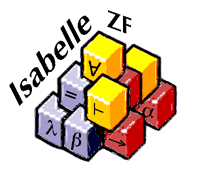
\includegraphics[scale=0.5]{isabelle_zf} \\[4ex] 
       Isabelle's Logics: FOL and ZF}

\author{{\em Lawrence C. Paulson}\\
        Computer Laboratory \\ University of Cambridge \\
        \texttt{lcp@cl.cam.ac.uk}\\[3ex] 
        With Contributions by Tobias Nipkow and Markus Wenzel}

\newcommand\subcaption[1]{\par {\centering\normalsize\sc#1\par}\bigskip
  \hrule\bigskip}
\newenvironment{constants}{\begin{center}\small\begin{tabular}{rrrr}}{\end{tabular}\end{center}}

\let\ts=\thinspace

\makeindex

\underscoreoff

\setcounter{secnumdepth}{2} \setcounter{tocdepth}{2}  %% {secnumdepth}{2}???

\pagestyle{headings}
\sloppy
\binperiod     %%%treat . like a binary operator

\begin{document}
\maketitle 

\begin{abstract}
This manual describes Isabelle's formalizations of many-sorted first-order
logic (\texttt{FOL}) and Zermelo-Fraenkel set theory (\texttt{ZF}).  See the
\emph{Reference Manual} for general Isabelle commands, and \emph{Introduction
  to Isabelle} for an overall tutorial.

This manual is part of the earlier Isabelle documentation, 
which is somewhat superseded by the Isabelle/HOL
\emph{Tutorial}~\cite{isa-tutorial}. However, the present document is the
only available documentation for Isabelle's versions of first-order logic
and set theory. Much of it is concerned with 
the primitives for conducting proofs 
using the ML top level.  It has been rewritten to use the Isar proof
language, but evidence of the old \ML{} orientation remains.
\end{abstract}


\subsubsection*{Acknowledgements} 
Markus Wenzel made numerous improvements.
    Philippe de Groote contributed to~ZF.  Philippe No\"el and
    Martin Coen made many contributions to~ZF.  The research has 
    been funded by the EPSRC (grants GR/G53279, GR/H40570, GR/K57381,
    GR/K77051, GR/M75440) and by ESPRIT (projects 3245:
    Logical Frameworks, and 6453: Types) and by the DFG Schwerpunktprogramm
    \emph{Deduktion}.
    
\pagenumbering{roman} \tableofcontents \cleardoublepage
\pagenumbering{arabic} 
\setcounter{page}{1} 

\chapter{Syntax primitives}

The rather generic framework of Isabelle/Isar syntax emerges from three main
syntactic categories: \emph{commands} of the top-level Isar engine (covering
theory and proof elements), \emph{methods} for general goal refinements
(analogous to traditional ``tactics''), and \emph{attributes} for operations
on facts (within a certain context).  Here we give a reference of basic
syntactic entities underlying Isabelle/Isar syntax in a bottom-up manner.
Concrete theory and proof language elements will be introduced later on.

\medskip

In order to get started with writing well-formed Isabelle/Isar documents, the
most important aspect to be noted is the difference of \emph{inner} versus
\emph{outer} syntax.  Inner syntax is that of Isabelle types and terms of the
logic, while outer syntax is that of Isabelle/Isar theory sources (including
proofs).  As a general rule, inner syntax entities may occur only as
\emph{atomic entities} within outer syntax.  For example, the string
\texttt{"x + y"} and identifier \texttt{z} are legal term specifications
within a theory, while \texttt{x + y} is not.

\begin{warn}
  Old-style Isabelle theories used to fake parts of the inner syntax of types,
  with rather complicated rules when quotes may be omitted.  Despite the minor
  drawback of requiring quotes more often, the syntax of Isabelle/Isar is
  somewhat simpler and more robust in that respect.
\end{warn}

Printed theory documents usually omit quotes to gain readability (this is a
matter of {\LaTeX} macro setup, say via \verb,\isabellestyle,, see also
\cite{isabelle-sys}).  Experienced users of Isabelle/Isar may easily
reconstruct the lost technical information, while mere readers need not care
about quotes at all.

\medskip

Isabelle/Isar input may contain any number of input termination characters
``\texttt{;}'' (semicolon) to separate commands explicitly.  This is
particularly useful in interactive shell sessions to make clear where the
current command is intended to end.  Otherwise, the interpreter loop will
continue to issue a secondary prompt ``\verb,#,'' until an end-of-command is
clearly recognized from the input syntax, e.g.\ encounter of the next command
keyword.

Advanced interfaces such as Proof~General \cite{proofgeneral} do not require
explicit semicolons, the amount of input text is determined automatically by
inspecting the present content of the Emacs text buffer.  In the printed
presentation of Isabelle/Isar documents semicolons are omitted altogether for
readability.

\begin{warn}
  Proof~General requires certain syntax classification tables in order to
  achieve properly synchronized interaction with the Isabelle/Isar process.
  These tables need to be consistent with the Isabelle version and particular
  logic image to be used in a running session (common object-logics may well
  change the outer syntax).  The standard setup should work correctly with any
  of the ``official'' logic images derived from Isabelle/HOL (including HOLCF
  etc.).  Users of alternative logics may need to tell Proof~General
  explicitly, e.g.\ by giving an option \verb,-k ZF, (in conjunction with
  \verb,-l ZF, to specify the default logic image).
\end{warn}

\section{Lexical matters}\label{sec:lex-syntax}

The Isabelle/Isar outer syntax provides token classes as presented below; most
of these coincide with the inner lexical syntax as presented in
\cite{isabelle-ref}.

\indexoutertoken{ident}\indexoutertoken{longident}\indexoutertoken{symident}
\indexoutertoken{nat}\indexoutertoken{var}\indexoutertoken{typefree}
\indexoutertoken{typevar}\indexoutertoken{string}\indexoutertoken{verbatim}
\begin{matharray}{rcl}
  ident & = & letter\,quasiletter^* \\
  longident & = & ident (\verb,.,ident)^+ \\
  symident & = & sym^+ ~|~ \verb,\<,ident\verb,>, \\
  nat & = & digit^+ \\
  var & = & ident ~|~ \verb,?,ident ~|~ \verb,?,ident\verb,.,nat \\
  typefree & = & \verb,',ident \\
  typevar & = & typefree ~|~ \verb,?,typefree ~|~ \verb,?,typefree\verb,.,nat \\
  string & = & \verb,", ~\dots~ \verb,", \\
  verbatim & = & \verb,{*, ~\dots~ \verb,*}, \\[1ex]

  letter & = & latin ~|~ \verb,\<,latin\verb,>, ~|~ \verb,\<,latin\,latin\verb,>, ~|~ greek ~|~ \\
         &   & \verb,\<^isub>, ~|~ \verb,\<^isup>, \\
  quasiletter & = & letter ~|~ digit ~|~ \verb,_, ~|~ \verb,', \\
  latin & = & \verb,a, ~|~ \dots ~|~ \verb,z, ~|~ \verb,A, ~|~ \dots ~|~ \verb,Z, \\
  digit & = & \verb,0, ~|~ \dots ~|~ \verb,9, \\
  sym & = & \verb,!, ~|~ \verb,#, ~|~ \verb,$, ~|~ \verb,%, ~|~ \verb,&, ~|~  %$
   \verb,*, ~|~ \verb,+, ~|~ \verb,-, ~|~ \verb,/, ~|~ \verb,:, ~|~ \\
  & & \verb,<, ~|~ \verb,=, ~|~ \verb,>, ~|~ \verb,?, ~|~ \texttt{\at} ~|~
  \verb,^, ~|~ \verb,_, ~|~ \verb,`, ~|~ \verb,|, ~|~ \verb,~, \\
greek & = & \verb,\<alpha>, ~|~ \verb,\<beta>, ~|~ \verb,\<gamma>, ~|~ \verb,\<delta>, ~| \\
      &   & \verb,\<epsilon>, ~|~ \verb,\<zeta>, ~|~ \verb,\<eta>, ~|~ \verb,\<theta>, ~| \\
      &   & \verb,\<iota>, ~|~ \verb,\<kappa>, ~|~ \verb,\<mu>, ~|~ \verb,\<nu>, ~| \\
      &   & \verb,\<xi>, ~|~ \verb,\<pi>, ~|~ \verb,\<rho>, ~|~ \verb,\<sigma>, ~| \\
      &   & \verb,\<tau>, ~|~ \verb,\<upsilon>, ~|~ \verb,\<phi>, ~|~ \verb,\<psi>, ~| \\
      &   & \verb,\<omega>, ~|~ \verb,\<Gamma>, ~|~ \verb,\<Delta>, ~|~ \verb,\<Theta>, ~| \\
      &   & \verb,\<Lambda>, ~|~ \verb,\<Xi>, ~|~ \verb,\<Pi>, ~|~ \verb,\<Sigma>, ~| \\
      &   & \verb,\<Upsilon>, ~|~ \verb,\<Phi>, ~|~ \verb,\<Psi>, ~|~ \verb,\<Omega>, \\
\end{matharray}

The syntax of $string$ admits any characters, including newlines; ``\verb|"|''
(double-quote) and ``\verb|\|'' (backslash) need to be escaped by a backslash.
The body of $verbatim$ may consist of any text not containing ``\verb|*}|'';
this allows convenient inclusion of quotes without further escapes.  The greek
letters do \emph{not} include \verb,\<lambda>,, which is already used
differently in the meta-logic.

Common mathematical symbols such as $\forall$ are represented in Isabelle as
\verb,\<forall>,.  There are infinitely many legal symbols like this, although
proper presentation is left to front-end tools such as {\LaTeX} or
Proof~General with the X-Symbol package.  A list of standard Isabelle symbols
that work well with these tools is given in \cite[appendix~A]{isabelle-sys}.

Comments take the form \texttt{(*~\dots~*)} and may be nested, although
user-interface tools may prevent this.  Note that \texttt{(*~\dots~*)}
indicate source comments only, which are stripped after lexical analysis of
the input.  The Isar document syntax also provides formal comments that are
considered as part of the text (see \S\ref{sec:comments}).

\begin{warn}
  Proof~General does not handle nested comments properly; it is also unable to
  keep \verb,(*,\,/\,\verb,{*, and \verb,*),\,/\,\verb,*}, apart, despite
  their rather different meaning.  These are inherent problems of Emacs
  legacy.  Users should not be overly aggressive about nesting or alternating
  these delimiters.
\end{warn}


\section{Common syntax entities}

Subsequently, we introduce several basic syntactic entities, such as names,
terms, and theorem specifications, which have been factored out of the actual
Isar language elements to be described later.

Note that some of the basic syntactic entities introduced below (e.g.\
\railqtok{name}) act much like tokens rather than plain nonterminals (e.g.\
\railnonterm{sort}), especially for the sake of error messages.  E.g.\ syntax
elements like $\CONSTS$ referring to \railqtok{name} or \railqtok{type} would
really report a missing name or type rather than any of the constituent
primitive tokens such as \railtok{ident} or \railtok{string}.


\subsection{Names}

Entity \railqtok{name} usually refers to any name of types, constants,
theorems etc.\ that are to be \emph{declared} or \emph{defined} (so qualified
identifiers are excluded here).  Quoted strings provide an escape for
non-identifier names or those ruled out by outer syntax keywords (e.g.\
\verb|"let"|).  Already existing objects are usually referenced by
\railqtok{nameref}.

\indexoutertoken{name}\indexoutertoken{parname}\indexoutertoken{nameref}
\indexoutertoken{int}
\begin{rail}
  name: ident | symident | string | nat
  ;
  parname: '(' name ')'
  ;
  nameref: name | longident
  ;
  int: nat | '-' nat
  ;
\end{rail}


\subsection{Comments}\label{sec:comments}

Large chunks of plain \railqtok{text} are usually given \railtok{verbatim},
i.e.\ enclosed in \verb|{*|~\dots~\verb|*}|.  For convenience, any of the
smaller text units conforming to \railqtok{nameref} are admitted as well.  A
marginal \railnonterm{comment} is of the form \texttt{--} \railqtok{text}.
Any number of these may occur within Isabelle/Isar commands.

\indexoutertoken{text}\indexouternonterm{comment}
\begin{rail}
  text: verbatim | nameref
  ;
  comment: '--' text
  ;
\end{rail}


\subsection{Type classes, sorts and arities}

Classes are specified by plain names.  Sorts have a very simple inner syntax,
which is either a single class name $c$ or a list $\{c@1, \dots, c@n\}$
referring to the intersection of these classes.  The syntax of type arities is
given directly at the outer level.

\railalias{subseteq}{\isasymsubseteq}
\railterm{subseteq}

\indexouternonterm{sort}\indexouternonterm{arity}
\indexouternonterm{classdecl}
\begin{rail}
  classdecl: name (('<' | subseteq) (nameref + ','))?
  ;
  sort: nameref
  ;
  arity: ('(' (sort + ',') ')')? sort
  ;
\end{rail}


\subsection{Types and terms}\label{sec:types-terms}

The actual inner Isabelle syntax, that of types and terms of the logic, is far
too sophisticated in order to be modelled explicitly at the outer theory
level.  Basically, any such entity has to be quoted to turn it into a single
token (the parsing and type-checking is performed internally later).  For
convenience, a slightly more liberal convention is adopted: quotes may be
omitted for any type or term that is already atomic at the outer level.  For
example, one may just write \texttt{x} instead of \texttt{"x"}.  Note that
symbolic identifiers (e.g.\ \texttt{++} or $\forall$) are available as well,
provided these have not been superseded by commands or other keywords already
(e.g.\ \texttt{=} or \texttt{+}).

\indexoutertoken{type}\indexoutertoken{term}\indexoutertoken{prop}
\begin{rail}
  type: nameref | typefree | typevar
  ;
  term: nameref | var
  ;
  prop: term
  ;
\end{rail}

Positional instantiations are indicated by giving a sequence of terms, or the
placeholder ``$\_$'' (underscore), which means to skip a position.

\indexoutertoken{inst}\indexoutertoken{insts}
\begin{rail}
  inst: underscore | term
  ;
  insts: (inst *)
  ;
\end{rail}

Type declarations and definitions usually refer to \railnonterm{typespec} on
the left-hand side.  This models basic type constructor application at the
outer syntax level.  Note that only plain postfix notation is available here,
but no infixes.

\indexouternonterm{typespec}
\begin{rail}
  typespec: (() | typefree | '(' ( typefree + ',' ) ')') name
  ;
\end{rail}


\subsection{Mixfix annotations}

Mixfix annotations specify concrete \emph{inner} syntax of Isabelle types and
terms.  Some commands such as $\TYPES$ (see \S\ref{sec:types-pure}) admit
infixes only, while $\CONSTS$ (see \S\ref{sec:consts}) and
$\isarkeyword{syntax}$ (see \S\ref{sec:syn-trans}) support the full range of
general mixfixes and binders.

\indexouternonterm{infix}\indexouternonterm{mixfix}\indexouternonterm{structmixfix}
\begin{rail}
  infix: '(' ('infix' | 'infixl' | 'infixr') string? nat ')'
  ;
  mixfix: infix | '(' string prios? nat? ')' | '(' 'binder' string prios? nat ')'
  ;
  structmixfix: mixfix | '(' 'structure' ')'
  ;

  prios: '[' (nat + ',') ']'
  ;
\end{rail}

Here the \railtok{string} specifications refer to the actual mixfix template
(see also \cite{isabelle-ref}), which may include literal text, spacing,
blocks, and arguments (denoted by ``$_$''); the special symbol \verb,\<index>,
(printed as ``\i'') represents an index argument that specifies an implicit
structure reference (see also \S\ref{sec:locale}).  Infix and binder
declarations provide common abbreviations for particular mixfix declarations.
So in practice, mixfix templates mostly degenerate to literal text for
concrete syntax, such as ``\verb,++,'' for an infix symbol, or ``\verb,++,\i''
for an infix of an implicit structure.



\subsection{Proof methods}\label{sec:syn-meth}

Proof methods are either basic ones, or expressions composed of methods via
``\texttt{,}'' (sequential composition), ``\texttt{|}'' (alternative choices),
``\texttt{?}'' (try), ``\texttt{+}'' (repeat at least once).  In practice,
proof methods are usually just a comma separated list of
\railqtok{nameref}~\railnonterm{args} specifications.  Note that parentheses
may be dropped for single method specifications (with no arguments).

\indexouternonterm{method}
\begin{rail}
  method: (nameref | '(' methods ')') (() | '?' | '+')
  ;
  methods: (nameref args | method) + (',' | '|')
  ;
\end{rail}

Proper use of Isar proof methods does \emph{not} involve goal addressing.
Nevertheless, specifying goal ranges may occasionally come in handy in
emulating tactic scripts.  Note that $[n-]$ refers to all goals, starting from
$n$.  All goals may be specified by $[!]$, which is the same as $[1-]$.

\indexouternonterm{goalspec}
\begin{rail}
  goalspec: '[' (nat '-' nat | nat '-' | nat | '!' ) ']'
  ;
\end{rail}


\subsection{Attributes and theorems}\label{sec:syn-att}

Attributes (and proof methods, see \S\ref{sec:syn-meth}) have their own
``semi-inner'' syntax, in the sense that input conforming to
\railnonterm{args} below is parsed by the attribute a second time.  The
attribute argument specifications may be any sequence of atomic entities
(identifiers, strings etc.), or properly bracketed argument lists.  Below
\railqtok{atom} refers to any atomic entity, including any \railtok{keyword}
conforming to \railtok{symident}.

\indexoutertoken{atom}\indexouternonterm{args}\indexouternonterm{attributes}
\begin{rail}
  atom: nameref | typefree | typevar | var | nat | keyword
  ;
  arg: atom | '(' args ')' | '[' args ']'
  ;
  args: arg *
  ;
  attributes: '[' (nameref args * ',') ']'
  ;
\end{rail}

Theorem specifications come in several flavors: \railnonterm{axmdecl} and
\railnonterm{thmdecl} usually refer to axioms, assumptions or results of goal
statements, while \railnonterm{thmdef} collects lists of existing theorems.
Existing theorems are given by \railnonterm{thmref} and \railnonterm{thmrefs},
the former requires an actual singleton result.  An optional index selection
specifies the individual theorems to be picked out of a given fact list.  Any
kind of theorem specification may include lists of attributes both on the left
and right hand sides; attributes are applied to any immediately preceding
fact.  If names are omitted, the theorems are not stored within the theorem
database of the theory or proof context, but any given attributes are applied
nonetheless.

\indexouternonterm{axmdecl}\indexouternonterm{thmdecl}
\indexouternonterm{thmdef}\indexouternonterm{thmref}
\indexouternonterm{thmrefs}\indexouternonterm{selection}
\begin{rail}
  axmdecl: name attributes? ':'
  ;
  thmdecl: thmbind ':'
  ;
  thmdef: thmbind '='
  ;
  thmref: nameref selection? attributes?
  ;
  thmrefs: thmref +
  ;

  thmbind: name attributes | name | attributes
  ;
  selection: '(' ((nat | nat '-' nat?) + ',') ')'
  ;
\end{rail}


\subsection{Term patterns and declarations}\label{sec:term-decls}

Wherever explicit propositions (or term fragments) occur in a proof text,
casual binding of schematic term variables may be given specified via patterns
of the form ``$\ISS{p@1\;\dots}{p@n}$''.  There are separate versions
available for \railqtok{term}s and \railqtok{prop}s.  The latter provides a
$\CONCLNAME$ part with patterns referring the (atomic) conclusion of a rule.

\indexouternonterm{termpat}\indexouternonterm{proppat}
\begin{rail}
  termpat: '(' ('is' term +) ')'
  ;
  proppat: '(' (('is' prop +) | 'concl' ('is' prop +) | ('is' prop +) 'concl' ('is' prop +)) ')'
  ;
\end{rail}

Declarations of local variables $x :: \tau$ and logical propositions $a :
\phi$ represent different views on the same principle of introducing a local
scope.  In practice, one may usually omit the typing of $vars$ (due to
type-inference), and the naming of propositions (due to implicit references of
current facts).  In any case, Isar proof elements usually admit to introduce
multiple such items simultaneously.

\indexouternonterm{vars}\indexouternonterm{props}
\begin{rail}
  vars: (name+) ('::' type)?
  ;
  props: thmdecl? (prop proppat? +)
  ;
\end{rail}

The treatment of multiple declarations corresponds to the complementary focus
of $vars$ versus $props$: in ``$x@1~\dots~x@n :: \tau$'' the typing refers to
all variables, while in $a\colon \phi@1~\dots~\phi@n$ the naming refers to all
propositions collectively.  Isar language elements that refer to $vars$ or
$props$ typically admit separate typings or namings via another level of
iteration, with explicit $\AND$ separators; e.g.\ see $\FIXNAME$ and
$\ASSUMENAME$ in \S\ref{sec:proof-context}.


\subsection{Antiquotations}\label{sec:antiq}

\begin{matharray}{rcl@{\hspace*{2cm}}rcl}
  thm & : & \isarantiq & text & : & \isarantiq \\
  prop & : & \isarantiq & goals & : & \isarantiq \\
  term & : & \isarantiq & subgoals & : & \isarantiq \\
  const & : & \isarantiq & prf & : & \isarantiq \\
  typeof & : & \isarantiq & full_prf & : & \isarantiq \\
  typ & : & \isarantiq \\  
  thm_style & : & \isarantiq \\  
  term_style & : & \isarantiq \\  
\end{matharray}

The text body of formal comments (see also \S\ref{sec:comments}) may contain
antiquotations of logical entities, such as theorems, terms and types, which
are to be presented in the final output produced by the Isabelle document
preparation system (see also \S\ref{sec:document-prep}).

Thus embedding of
``\texttt{{\at}{\ttlbrace}term~[show_types]~"f(x)~=~a~+~x"{\ttrbrace}}''
within a text block would cause
\isa{(f{\isasymColon}'a~{\isasymRightarrow}~'a)~(x{\isasymColon}'a)~=~(a{\isasymColon}'a)~+~x}
to appear in the final {\LaTeX} document.  Also note that theorem
antiquotations may involve attributes as well.  For example,
\texttt{{\at}{\ttlbrace}thm~sym~[no_vars]{\ttrbrace}} would print the
statement where all schematic variables have been replaced by fixed ones,
which are easier to read.

\indexisarant{thm}\indexisarant{prop}\indexisarant{term}\indexisarant{const}
\indexisarant{typeof}\indexisarant{typ}\indexisarant{thm-style}
\indexisarant{term-style}\indexisarant{text}\indexisarant{goals}
\indexisarant{subgoals}\indexisarant{prf}\indexisarant{full-prf}

\begin{rail}
  atsign lbrace antiquotation rbrace
  ;

  antiquotation:
    'thm' options thmrefs |
    'prop' options prop |
    'term' options term |
    'const' options term |
    'typeof' options term |
    'typ' options type |
    'thm\_style' options style thmref |
    'term\_style' options style term |
    'text' options name |
    'goals' options |
    'subgoals' options |
    'prf' options thmrefs |
    'full\_prf' options thmrefs
  ;
  options: '[' (option * ',') ']'
  ;
  option: name | name '=' name
  ;
\end{rail}

Note that the syntax of antiquotations may \emph{not} include source comments
\texttt{(*~\dots~*)} or verbatim text \verb|{*|~\dots~\verb|*}|.

\begin{descr}

\item [$\at\{thm~\vec a\}$] prints theorems $\vec a$. Note that attribute
  specifications may be included as well (see also \S\ref{sec:syn-att}); the
  $no_vars$ operation (see \S\ref{sec:misc-meth-att}) would be particularly
  useful to suppress printing of schematic variables.

\item [$\at\{prop~\phi\}$] prints a well-typed proposition $\phi$.

\item [$\at\{term~t\}$] prints a well-typed term $t$.

\item [$\at\{const~c\}$] prints a well-defined constant $c$.

\item [$\at\{typeof~t\}$] prints the type of a well-typed term $t$.

\item [$\at\{typ~\tau\}$] prints a well-formed type $\tau$.

\item [$\at\{thm_style~s~a\}$] prints theorem $a$, previously
  applying a style $s$ to it; otherwise behaves the same as $\at\{thm~a\}$
  with just one theorem.

\item [$\at\{term_style~s~t\}$] prints a well-typed term $t$, previously
  applying a style $s$ to it; otherwise behaves the same as $\at\{term~t\}$.

\item [$\at\{text~s\}$] prints uninterpreted source text $s$.  This is
  particularly useful to print portions of text according to the Isabelle
  {\LaTeX} output style, without demanding well-formedness (e.g.\ small pieces
  of terms that should not be parsed or type-checked yet).

\item [$\at\{goals\}$] prints the current \emph{dynamic} goal state.  This is
  mainly for support of tactic-emulation scripts within Isar --- presentation
  of goal states does not conform to actual human-readable proof documents.
  Please do not include goal states into document output unless you really
  know what you are doing!

\item [$\at\{subgoals\}$] behaves almost like $goals$, except that it does not
  print the main goal.

\item [$\at\{prf~\vec a\}$] prints the (compact) proof terms corresponding to
  the theorems $\vec a$. Note that this
  requires proof terms to be switched on for the current object logic
  (see the ``Proof terms'' section of the Isabelle reference manual
  for information on how to do this).

\item [$\at\{full_prf~\vec a\}$] is like $\at\{prf~\vec a\}$, but displays
  the full proof terms, i.e.\ also displays information omitted in
  the compact proof term, which is denoted by ``$_$'' placeholders there.

\end{descr}

There are a few standard styles for use with $\at\{thm_style~s~a\}$ and
$\at\{term_style~s~t\}$:

\begin{descr}
  
\item [$lhs$] extracts the first argument of any application form with at
  least two arguments -- typically is meta-level or object-level equality or
  any other binary relation.
  
\item [$rhs$] similar to $lhs$, but extracts the second argument.
  
\item [$conlusion$] extracts the conclusion $C$ from nested meta-level
  implications $A@1 \Imp \cdots A@n \Imp C$.

\end{descr}

Further styles may be defined at ML level.

\medskip

The following options are available to tune the output.  Note that most of
these coincide with ML flags of the same names (see also \cite{isabelle-ref}).
\begin{descr}
\item[$show_types = bool$ and $show_sorts = bool$] control printing of
  explicit type and sort constraints.
\item[$show_structs = bool$] controls printing of implicit structures.
\item[$long_names = bool$] forces names of types and constants etc.\ to be
  printed in their fully qualified internal form.
\item[$eta_contract = bool$] prints terms in $\eta$-contracted form.
\item[$display = bool$] indicates if the text is to be output as multi-line
  ``display material'', rather than a small piece of text without line breaks
  (which is the default).
\item[$breaks = bool$] controls line breaks in non-display material.
\item[$quotes = bool$] indicates if the output should be enclosed in double
  quotes.
\item[$mode = name$] adds $name$ to the print mode to be used for presentation
  (see also \cite{isabelle-ref}).  Note that the standard setup for {\LaTeX}
  output is already present by default, including the modes ``$latex$'',
  ``$xsymbols$'', ``$symbols$''.
\item[$margin = nat$ and $indent = nat$] change the margin or indentation for
  pretty printing of display material.
\item[$source = bool$] prints the source text of the antiquotation arguments,
  rather than the actual value.  Note that this does not affect
  well-formedness checks of $thm$, $term$, etc. (only the $text$ antiquotation
  admits arbitrary output).
\item[$goals_limit = nat$] determines the maximum number of goals to be
  printed.
\item[$locale = name$] specifies an alternative context used for evaluating
  and printing the subsequent argument.
\end{descr}

For boolean flags, ``$name = true$'' may be abbreviated as ``$name$''.  All of
the above flags are disabled by default, unless changed from ML.

\medskip Note that antiquotations do not only spare the author from tedious
typing of logical entities, but also achieve some degree of
consistency-checking of informal explanations with formal developments:
well-formedness of terms and types with respect to the current theory or proof
context is ensured here.

%%% Local Variables:
%%% mode: latex
%%% TeX-master: "isar-ref"
%%% End:

%% $Id$
\chapter{First-Order Logic}
\index{first-order logic|(}

Isabelle implements Gentzen's natural deduction systems {\sc nj} and {\sc
  nk}.  Intuitionistic first-order logic is defined first, as theory
\thydx{IFOL}.  Classical logic, theory \thydx{FOL}, is
obtained by adding the double negation rule.  Basic proof procedures are
provided.  The intuitionistic prover works with derived rules to simplify
implications in the assumptions.  Classical~\texttt{FOL} employs Isabelle's
classical reasoner, which simulates a sequent calculus.

\section{Syntax and rules of inference}
The logic is many-sorted, using Isabelle's type classes.  The class of
first-order terms is called \cldx{term} and is a subclass of \texttt{logic}.
No types of individuals are provided, but extensions can define types such
as \texttt{nat::term} and type constructors such as \texttt{list::(term)term}
(see the examples directory, \texttt{FOL/ex}).  Below, the type variable
$\alpha$ ranges over class \texttt{term}; the equality symbol and quantifiers
are polymorphic (many-sorted).  The type of formulae is~\tydx{o}, which
belongs to class~\cldx{logic}.  Figure~\ref{fol-syntax} gives the syntax.
Note that $a$\verb|~=|$b$ is translated to $\neg(a=b)$.

Figure~\ref{fol-rules} shows the inference rules with their~\ML\ names.
Negation is defined in the usual way for intuitionistic logic; $\neg P$
abbreviates $P\imp\bot$.  The biconditional~($\bimp$) is defined through
$\conj$ and~$\imp$; introduction and elimination rules are derived for it.

The unique existence quantifier, $\exists!x.P(x)$, is defined in terms
of~$\exists$ and~$\forall$.  An Isabelle binder, it admits nested
quantifications.  For instance, $\exists!x\;y.P(x,y)$ abbreviates
$\exists!x. \exists!y.P(x,y)$; note that this does not mean that there
exists a unique pair $(x,y)$ satisfying~$P(x,y)$.

Some intuitionistic derived rules are shown in
Fig.\ts\ref{fol-int-derived}, again with their \ML\ names.  These include
rules for the defined symbols $\neg$, $\bimp$ and $\exists!$.  Natural
deduction typically involves a combination of forward and backward
reasoning, particularly with the destruction rules $(\conj E)$,
$({\imp}E)$, and~$(\forall E)$.  Isabelle's backward style handles these
rules badly, so sequent-style rules are derived to eliminate conjunctions,
implications, and universal quantifiers.  Used with elim-resolution,
\tdx{allE} eliminates a universal quantifier while \tdx{all_dupE}
re-inserts the quantified formula for later use.  The rules {\tt
conj_impE}, etc., support the intuitionistic proof procedure
(see~\S\ref{fol-int-prover}).

See the files \texttt{FOL/IFOL.thy}, \texttt{FOL/IFOL.ML} and
\texttt{FOL/intprover.ML} for complete listings of the rules and
derived rules.

\begin{figure} 
\begin{center}
\begin{tabular}{rrr} 
  \it name      &\it meta-type  & \it description \\ 
  \cdx{Trueprop}& $o\To prop$           & coercion to $prop$\\
  \cdx{Not}     & $o\To o$              & negation ($\neg$) \\
  \cdx{True}    & $o$                   & tautology ($\top$) \\
  \cdx{False}   & $o$                   & absurdity ($\bot$)
\end{tabular}
\end{center}
\subcaption{Constants}

\begin{center}
\begin{tabular}{llrrr} 
  \it symbol &\it name     &\it meta-type & \it priority & \it description \\
  \sdx{ALL}  & \cdx{All}  & $(\alpha\To o)\To o$ & 10 & 
        universal quantifier ($\forall$) \\
  \sdx{EX}   & \cdx{Ex}   & $(\alpha\To o)\To o$ & 10 & 
        existential quantifier ($\exists$) \\
  \texttt{EX!}  & \cdx{Ex1}  & $(\alpha\To o)\To o$ & 10 & 
        unique existence ($\exists!$)
\end{tabular}
\index{*"E"X"! symbol}
\end{center}
\subcaption{Binders} 

\begin{center}
\index{*"= symbol}
\index{&@{\tt\&} symbol}
\index{*"| symbol}
\index{*"-"-"> symbol}
\index{*"<"-"> symbol}
\begin{tabular}{rrrr} 
  \it symbol    & \it meta-type         & \it priority & \it description \\ 
  \tt =         & $[\alpha,\alpha]\To o$ & Left 50 & equality ($=$) \\
  \tt \&        & $[o,o]\To o$          & Right 35 & conjunction ($\conj$) \\
  \tt |         & $[o,o]\To o$          & Right 30 & disjunction ($\disj$) \\
  \tt -->       & $[o,o]\To o$          & Right 25 & implication ($\imp$) \\
  \tt <->       & $[o,o]\To o$          & Right 25 & biconditional ($\bimp$) 
\end{tabular}
\end{center}
\subcaption{Infixes}

\dquotes
\[\begin{array}{rcl}
 formula & = & \hbox{expression of type~$o$} \\
         & | & term " = " term \quad| \quad term " \ttilde= " term \\
         & | & "\ttilde\ " formula \\
         & | & formula " \& " formula \\
         & | & formula " | " formula \\
         & | & formula " --> " formula \\
         & | & formula " <-> " formula \\
         & | & "ALL~" id~id^* " . " formula \\
         & | & "EX~~" id~id^* " . " formula \\
         & | & "EX!~" id~id^* " . " formula
  \end{array}
\]
\subcaption{Grammar}
\caption{Syntax of \texttt{FOL}} \label{fol-syntax}
\end{figure}


\begin{figure} 
\begin{ttbox}
\tdx{refl}        a=a
\tdx{subst}       [| a=b;  P(a) |] ==> P(b)
\subcaption{Equality rules}

\tdx{conjI}       [| P;  Q |] ==> P&Q
\tdx{conjunct1}   P&Q ==> P
\tdx{conjunct2}   P&Q ==> Q

\tdx{disjI1}      P ==> P|Q
\tdx{disjI2}      Q ==> P|Q
\tdx{disjE}       [| P|Q;  P ==> R;  Q ==> R |] ==> R

\tdx{impI}        (P ==> Q) ==> P-->Q
\tdx{mp}          [| P-->Q;  P |] ==> Q

\tdx{FalseE}      False ==> P
\subcaption{Propositional rules}

\tdx{allI}        (!!x. P(x))  ==> (ALL x.P(x))
\tdx{spec}        (ALL x.P(x)) ==> P(x)

\tdx{exI}         P(x) ==> (EX x.P(x))
\tdx{exE}         [| EX x.P(x);  !!x. P(x) ==> R |] ==> R
\subcaption{Quantifier rules}

\tdx{True_def}    True        == False-->False
\tdx{not_def}     ~P          == P-->False
\tdx{iff_def}     P<->Q       == (P-->Q) & (Q-->P)
\tdx{ex1_def}     EX! x. P(x) == EX x. P(x) & (ALL y. P(y) --> y=x)
\subcaption{Definitions}
\end{ttbox}

\caption{Rules of intuitionistic logic} \label{fol-rules}
\end{figure}


\begin{figure} 
\begin{ttbox}
\tdx{sym}       a=b ==> b=a
\tdx{trans}     [| a=b;  b=c |] ==> a=c
\tdx{ssubst}    [| b=a;  P(a) |] ==> P(b)
\subcaption{Derived equality rules}

\tdx{TrueI}     True

\tdx{notI}      (P ==> False) ==> ~P
\tdx{notE}      [| ~P;  P |] ==> R

\tdx{iffI}      [| P ==> Q;  Q ==> P |] ==> P<->Q
\tdx{iffE}      [| P <-> Q;  [| P-->Q; Q-->P |] ==> R |] ==> R
\tdx{iffD1}     [| P <-> Q;  P |] ==> Q            
\tdx{iffD2}     [| P <-> Q;  Q |] ==> P

\tdx{ex1I}      [| P(a);  !!x. P(x) ==> x=a |]  ==>  EX! x. P(x)
\tdx{ex1E}      [| EX! x.P(x);  !!x.[| P(x);  ALL y. P(y) --> y=x |] ==> R 
          |] ==> R
\subcaption{Derived rules for \(\top\), \(\neg\), \(\bimp\) and \(\exists!\)}

\tdx{conjE}     [| P&Q;  [| P; Q |] ==> R |] ==> R
\tdx{impE}      [| P-->Q;  P;  Q ==> R |] ==> R
\tdx{allE}      [| ALL x.P(x);  P(x) ==> R |] ==> R
\tdx{all_dupE}  [| ALL x.P(x);  [| P(x); ALL x.P(x) |] ==> R |] ==> R
\subcaption{Sequent-style elimination rules}

\tdx{conj_impE} [| (P&Q)-->S;  P-->(Q-->S) ==> R |] ==> R
\tdx{disj_impE} [| (P|Q)-->S;  [| P-->S; Q-->S |] ==> R |] ==> R
\tdx{imp_impE}  [| (P-->Q)-->S;  [| P; Q-->S |] ==> Q;  S ==> R |] ==> R
\tdx{not_impE}  [| ~P --> S;  P ==> False;  S ==> R |] ==> R
\tdx{iff_impE}  [| (P<->Q)-->S; [| P; Q-->S |] ==> Q; [| Q; P-->S |] ==> P;
             S ==> R |] ==> R
\tdx{all_impE}  [| (ALL x.P(x))-->S;  !!x.P(x);  S ==> R |] ==> R
\tdx{ex_impE}   [| (EX x.P(x))-->S;  P(a)-->S ==> R |] ==> R
\end{ttbox}
\subcaption{Intuitionistic simplification of implication}
\caption{Derived rules for intuitionistic logic} \label{fol-int-derived}
\end{figure}


\section{Generic packages}
FOL instantiates most of Isabelle's generic packages.
\begin{itemize}
\item 
It instantiates the simplifier.  Both equality ($=$) and the biconditional
($\bimp$) may be used for rewriting.  Tactics such as \texttt{Asm_simp_tac} and
\texttt{Full_simp_tac} refer to the default simpset (\texttt{simpset()}), which works for
most purposes.  Named simplification sets include \ttindexbold{IFOL_ss},
for intuitionistic first-order logic, and \ttindexbold{FOL_ss},
for classical logic.  See the file
\texttt{FOL/simpdata.ML} for a complete listing of the simplification
rules%
\iflabelundefined{sec:setting-up-simp}{}%
        {, and \S\ref{sec:setting-up-simp} for discussion}.

\item 
It instantiates the classical reasoner.  See~\S\ref{fol-cla-prover}
for details. 

\item FOL provides the tactic \ttindex{hyp_subst_tac}, which substitutes for
  an equality throughout a subgoal and its hypotheses.  This tactic uses FOL's
  general substitution rule.
\end{itemize}

\begin{warn}\index{simplification!of conjunctions}%
  Reducing $a=b\conj P(a)$ to $a=b\conj P(b)$ is sometimes advantageous.  The
  left part of a conjunction helps in simplifying the right part.  This effect
  is not available by default: it can be slow.  It can be obtained by
  including \ttindex{conj_cong} in a simpset, \verb$addcongs [conj_cong]$.
\end{warn}


\section{Intuitionistic proof procedures} \label{fol-int-prover}
Implication elimination (the rules~\texttt{mp} and~\texttt{impE}) pose
difficulties for automated proof.  In intuitionistic logic, the assumption
$P\imp Q$ cannot be treated like $\neg P\disj Q$.  Given $P\imp Q$, we may
use~$Q$ provided we can prove~$P$; the proof of~$P$ may require repeated
use of $P\imp Q$.  If the proof of~$P$ fails then the whole branch of the
proof must be abandoned.  Thus intuitionistic propositional logic requires
backtracking.  

For an elementary example, consider the intuitionistic proof of $Q$ from
$P\imp Q$ and $(P\imp Q)\imp P$.  The implication $P\imp Q$ is needed
twice:
\[ \infer[({\imp}E)]{Q}{P\imp Q &
       \infer[({\imp}E)]{P}{(P\imp Q)\imp P & P\imp Q}} 
\]
The theorem prover for intuitionistic logic does not use~\texttt{impE}.\@
Instead, it simplifies implications using derived rules
(Fig.\ts\ref{fol-int-derived}).  It reduces the antecedents of implications
to atoms and then uses Modus Ponens: from $P\imp Q$ and~$P$ deduce~$Q$.
The rules \tdx{conj_impE} and \tdx{disj_impE} are 
straightforward: $(P\conj Q)\imp S$ is equivalent to $P\imp (Q\imp S)$, and
$(P\disj Q)\imp S$ is equivalent to the conjunction of $P\imp S$ and $Q\imp
S$.  The other \ldots{\tt_impE} rules are unsafe; the method requires
backtracking.  All the rules are derived in the same simple manner.

Dyckhoff has independently discovered similar rules, and (more importantly)
has demonstrated their completeness for propositional
logic~\cite{dyckhoff}.  However, the tactics given below are not complete
for first-order logic because they discard universally quantified
assumptions after a single use.
\begin{ttbox} 
mp_tac              : int -> tactic
eq_mp_tac           : int -> tactic
IntPr.safe_step_tac : int -> tactic
IntPr.safe_tac      :        tactic
IntPr.inst_step_tac : int -> tactic
IntPr.step_tac      : int -> tactic
IntPr.fast_tac      : int -> tactic
IntPr.best_tac      : int -> tactic
\end{ttbox}
Most of these belong to the structure \texttt{IntPr} and resemble the
tactics of Isabelle's classical reasoner.

\begin{ttdescription}
\item[\ttindexbold{mp_tac} {\it i}] 
attempts to use \tdx{notE} or \tdx{impE} within the assumptions in
subgoal $i$.  For each assumption of the form $\neg P$ or $P\imp Q$, it
searches for another assumption unifiable with~$P$.  By
contradiction with $\neg P$ it can solve the subgoal completely; by Modus
Ponens it can replace the assumption $P\imp Q$ by $Q$.  The tactic can
produce multiple outcomes, enumerating all suitable pairs of assumptions.

\item[\ttindexbold{eq_mp_tac} {\it i}] 
is like \texttt{mp_tac} {\it i}, but may not instantiate unknowns --- thus, it
is safe.

\item[\ttindexbold{IntPr.safe_step_tac} $i$] performs a safe step on
subgoal~$i$.  This may include proof by assumption or Modus Ponens (taking
care not to instantiate unknowns), or \texttt{hyp_subst_tac}. 

\item[\ttindexbold{IntPr.safe_tac}] repeatedly performs safe steps on all 
subgoals.  It is deterministic, with at most one outcome.

\item[\ttindexbold{IntPr.inst_step_tac} $i$] is like \texttt{safe_step_tac},
but allows unknowns to be instantiated.

\item[\ttindexbold{IntPr.step_tac} $i$] tries \texttt{safe_tac} or {\tt
    inst_step_tac}, or applies an unsafe rule.  This is the basic step of
  the intuitionistic proof procedure.

\item[\ttindexbold{IntPr.fast_tac} $i$] applies \texttt{step_tac}, using
depth-first search, to solve subgoal~$i$.

\item[\ttindexbold{IntPr.best_tac} $i$] applies \texttt{step_tac}, using
best-first search (guided by the size of the proof state) to solve subgoal~$i$.
\end{ttdescription}
Here are some of the theorems that \texttt{IntPr.fast_tac} proves
automatically.  The latter three date from {\it Principia Mathematica}
(*11.53, *11.55, *11.61)~\cite{principia}.
\begin{ttbox}
~~P & ~~(P --> Q) --> ~~Q
(ALL x y. P(x) --> Q(y)) <-> ((EX x. P(x)) --> (ALL y. Q(y)))
(EX x y. P(x) & Q(x,y)) <-> (EX x. P(x) & (EX y. Q(x,y)))
(EX y. ALL x. P(x) --> Q(x,y)) --> (ALL x. P(x) --> (EX y. Q(x,y)))
\end{ttbox}



\begin{figure} 
\begin{ttbox}
\tdx{excluded_middle}    ~P | P

\tdx{disjCI}    (~Q ==> P) ==> P|Q
\tdx{exCI}      (ALL x. ~P(x) ==> P(a)) ==> EX x.P(x)
\tdx{impCE}     [| P-->Q; ~P ==> R; Q ==> R |] ==> R
\tdx{iffCE}     [| P<->Q;  [| P; Q |] ==> R;  [| ~P; ~Q |] ==> R |] ==> R
\tdx{notnotD}   ~~P ==> P
\tdx{swap}      ~P ==> (~Q ==> P) ==> Q
\end{ttbox}
\caption{Derived rules for classical logic} \label{fol-cla-derived}
\end{figure}


\section{Classical proof procedures} \label{fol-cla-prover}
The classical theory, \thydx{FOL}, consists of intuitionistic logic plus
the rule
$$ \vcenter{\infer{P}{\infer*{P}{[\neg P]}}} \eqno(classical) $$
\noindent
Natural deduction in classical logic is not really all that natural.  FOL
derives classical introduction rules for $\disj$ and~$\exists$, as well as
classical elimination rules for~$\imp$ and~$\bimp$, and the swap rule (see
Fig.\ts\ref{fol-cla-derived}).

The classical reasoner is installed.  Tactics such as \texttt{Blast_tac} and {\tt
Best_tac} refer to the default claset (\texttt{claset()}), which works for most
purposes.  Named clasets include \ttindexbold{prop_cs}, which includes the
propositional rules, and \ttindexbold{FOL_cs}, which also includes quantifier
rules.  See the file \texttt{FOL/cladata.ML} for lists of the
classical rules, and 
\iflabelundefined{chap:classical}{the {\em Reference Manual\/}}%
        {Chap.\ts\ref{chap:classical}} 
for more discussion of classical proof methods.


\section{An intuitionistic example}
Here is a session similar to one in {\em Logic and Computation}
\cite[pages~222--3]{paulson87}.  Isabelle treats quantifiers differently
from {\sc lcf}-based theorem provers such as {\sc hol}.  

First, we specify that we are working in intuitionistic logic:
\begin{ttbox}
context IFOL.thy;
\end{ttbox}
The proof begins by entering the goal, then applying the rule $({\imp}I)$.
\begin{ttbox}
Goal "(EX y. ALL x. Q(x,y)) -->  (ALL x. EX y. Q(x,y))";
{\out Level 0}
{\out (EX y. ALL x. Q(x,y)) --> (ALL x. EX y. Q(x,y))}
{\out  1. (EX y. ALL x. Q(x,y)) --> (ALL x. EX y. Q(x,y))}
\ttbreak
by (resolve_tac [impI] 1);
{\out Level 1}
{\out (EX y. ALL x. Q(x,y)) --> (ALL x. EX y. Q(x,y))}
{\out  1. EX y. ALL x. Q(x,y) ==> ALL x. EX y. Q(x,y)}
\end{ttbox}
In this example, we shall never have more than one subgoal.  Applying
$({\imp}I)$ replaces~\verb|-->| by~\verb|==>|, making
\(\ex{y}\all{x}Q(x,y)\) an assumption.  We have the choice of
$({\exists}E)$ and $({\forall}I)$; let us try the latter.
\begin{ttbox}
by (resolve_tac [allI] 1);
{\out Level 2}
{\out (EX y. ALL x. Q(x,y)) --> (ALL x. EX y. Q(x,y))}
{\out  1. !!x. EX y. ALL x. Q(x,y) ==> EX y. Q(x,y)}
\end{ttbox}
Applying $({\forall}I)$ replaces the \texttt{ALL~x} by \hbox{\tt!!x},
changing the universal quantifier from object~($\forall$) to
meta~($\Forall$).  The bound variable is a {\bf parameter} of the
subgoal.  We now must choose between $({\exists}I)$ and $({\exists}E)$.  What
happens if the wrong rule is chosen?
\begin{ttbox}
by (resolve_tac [exI] 1);
{\out Level 3}
{\out (EX y. ALL x. Q(x,y)) --> (ALL x. EX y. Q(x,y))}
{\out  1. !!x. EX y. ALL x. Q(x,y) ==> Q(x,?y2(x))}
\end{ttbox}
The new subgoal~1 contains the function variable {\tt?y2}.  Instantiating
{\tt?y2} can replace~{\tt?y2(x)} by a term containing~\texttt{x}, even
though~\texttt{x} is a bound variable.  Now we analyse the assumption
\(\exists y.\forall x. Q(x,y)\) using elimination rules:
\begin{ttbox}
by (eresolve_tac [exE] 1);
{\out Level 4}
{\out (EX y. ALL x. Q(x,y)) --> (ALL x. EX y. Q(x,y))}
{\out  1. !!x y. ALL x. Q(x,y) ==> Q(x,?y2(x))}
\end{ttbox}
Applying $(\exists E)$ has produced the parameter \texttt{y} and stripped the
existential quantifier from the assumption.  But the subgoal is unprovable:
there is no way to unify \texttt{?y2(x)} with the bound variable~\texttt{y}.
Using \texttt{choplev} we can return to the critical point.  This time we
apply $({\exists}E)$:
\begin{ttbox}
choplev 2;
{\out Level 2}
{\out (EX y. ALL x. Q(x,y)) --> (ALL x. EX y. Q(x,y))}
{\out  1. !!x. EX y. ALL x. Q(x,y) ==> EX y. Q(x,y)}
\ttbreak
by (eresolve_tac [exE] 1);
{\out Level 3}
{\out (EX y. ALL x. Q(x,y)) --> (ALL x. EX y. Q(x,y))}
{\out  1. !!x y. ALL x. Q(x,y) ==> EX y. Q(x,y)}
\end{ttbox}
We now have two parameters and no scheme variables.  Applying
$({\exists}I)$ and $({\forall}E)$ produces two scheme variables, which are
applied to those parameters.  Parameters should be produced early, as this
example demonstrates.
\begin{ttbox}
by (resolve_tac [exI] 1);
{\out Level 4}
{\out (EX y. ALL x. Q(x,y)) --> (ALL x. EX y. Q(x,y))}
{\out  1. !!x y. ALL x. Q(x,y) ==> Q(x,?y3(x,y))}
\ttbreak
by (eresolve_tac [allE] 1);
{\out Level 5}
{\out (EX y. ALL x. Q(x,y)) --> (ALL x. EX y. Q(x,y))}
{\out  1. !!x y. Q(?x4(x,y),y) ==> Q(x,?y3(x,y))}
\end{ttbox}
The subgoal has variables \texttt{?y3} and \texttt{?x4} applied to both
parameters.  The obvious projection functions unify {\tt?x4(x,y)} with~{\tt
x} and \verb|?y3(x,y)| with~\texttt{y}.
\begin{ttbox}
by (assume_tac 1);
{\out Level 6}
{\out (EX y. ALL x. Q(x,y)) --> (ALL x. EX y. Q(x,y))}
{\out No subgoals!}
\end{ttbox}
The theorem was proved in six tactic steps, not counting the abandoned
ones.  But proof checking is tedious; \ttindex{IntPr.fast_tac} proves the
theorem in one step.
\begin{ttbox}
Goal "(EX y. ALL x. Q(x,y)) -->  (ALL x. EX y. Q(x,y))";
{\out Level 0}
{\out (EX y. ALL x. Q(x,y)) --> (ALL x. EX y. Q(x,y))}
{\out  1. (EX y. ALL x. Q(x,y)) --> (ALL x. EX y. Q(x,y))}
by (IntPr.fast_tac 1);
{\out Level 1}
{\out (EX y. ALL x. Q(x,y)) --> (ALL x. EX y. Q(x,y))}
{\out No subgoals!}
\end{ttbox}


\section{An example of intuitionistic negation}
The following example demonstrates the specialized forms of implication
elimination.  Even propositional formulae can be difficult to prove from
the basic rules; the specialized rules help considerably.  

Propositional examples are easy to invent.  As Dummett notes~\cite[page
28]{dummett}, $\neg P$ is classically provable if and only if it is
intuitionistically provable;  therefore, $P$ is classically provable if and
only if $\neg\neg P$ is intuitionistically provable.%
\footnote{Of course this holds only for propositional logic, not if $P$ is
  allowed to contain quantifiers.} Proving $\neg\neg P$ intuitionistically is
much harder than proving~$P$ classically.

Our example is the double negation of the classical tautology $(P\imp
Q)\disj (Q\imp P)$.  When stating the goal, we command Isabelle to expand
negations to implications using the definition $\neg P\equiv P\imp\bot$.
This allows use of the special implication rules.
\begin{ttbox}
Goalw [not_def] "~ ~ ((P-->Q) | (Q-->P))";
{\out Level 0}
{\out ~ ~ ((P --> Q) | (Q --> P))}
{\out  1. ((P --> Q) | (Q --> P) --> False) --> False}
\end{ttbox}
The first step is trivial.
\begin{ttbox}
by (resolve_tac [impI] 1);
{\out Level 1}
{\out ~ ~ ((P --> Q) | (Q --> P))}
{\out  1. (P --> Q) | (Q --> P) --> False ==> False}
\end{ttbox}
By $(\imp E)$ it would suffice to prove $(P\imp Q)\disj (Q\imp P)$, but
that formula is not a theorem of intuitionistic logic.  Instead we apply
the specialized implication rule \tdx{disj_impE}.  It splits the
assumption into two assumptions, one for each disjunct.
\begin{ttbox}
by (eresolve_tac [disj_impE] 1);
{\out Level 2}
{\out ~ ~ ((P --> Q) | (Q --> P))}
{\out  1. [| (P --> Q) --> False; (Q --> P) --> False |] ==> False}
\end{ttbox}
We cannot hope to prove $P\imp Q$ or $Q\imp P$ separately, but
their negations are inconsistent.  Applying \tdx{imp_impE} breaks down
the assumption $\neg(P\imp Q)$, asking to show~$Q$ while providing new
assumptions~$P$ and~$\neg Q$.
\begin{ttbox}
by (eresolve_tac [imp_impE] 1);
{\out Level 3}
{\out ~ ~ ((P --> Q) | (Q --> P))}
{\out  1. [| (Q --> P) --> False; P; Q --> False |] ==> Q}
{\out  2. [| (Q --> P) --> False; False |] ==> False}
\end{ttbox}
Subgoal~2 holds trivially; let us ignore it and continue working on
subgoal~1.  Thanks to the assumption~$P$, we could prove $Q\imp P$;
applying \tdx{imp_impE} is simpler.
\begin{ttbox}
by (eresolve_tac [imp_impE] 1);
{\out Level 4}
{\out ~ ~ ((P --> Q) | (Q --> P))}
{\out  1. [| P; Q --> False; Q; P --> False |] ==> P}
{\out  2. [| P; Q --> False; False |] ==> Q}
{\out  3. [| (Q --> P) --> False; False |] ==> False}
\end{ttbox}
The three subgoals are all trivial.
\begin{ttbox}
by (REPEAT (eresolve_tac [FalseE] 2));
{\out Level 5}
{\out ~ ~ ((P --> Q) | (Q --> P))}
{\out  1. [| P; Q --> False; Q; P --> False |] ==> P}
\ttbreak
by (assume_tac 1);
{\out Level 6}
{\out ~ ~ ((P --> Q) | (Q --> P))}
{\out No subgoals!}
\end{ttbox}
This proof is also trivial for \texttt{IntPr.fast_tac}.


\section{A classical example} \label{fol-cla-example}
To illustrate classical logic, we shall prove the theorem
$\ex{y}\all{x}P(y)\imp P(x)$.  Informally, the theorem can be proved as
follows.  Choose~$y$ such that~$\neg P(y)$, if such exists; otherwise
$\all{x}P(x)$ is true.  Either way the theorem holds.  First, we switch to
classical logic:
\begin{ttbox}
context FOL.thy;
\end{ttbox}

The formal proof does not conform in any obvious way to the sketch given
above.  The key inference is the first one, \tdx{exCI}; this classical
version of~$(\exists I)$ allows multiple instantiation of the quantifier.
\begin{ttbox}
Goal "EX y. ALL x. P(y)-->P(x)";
{\out Level 0}
{\out EX y. ALL x. P(y) --> P(x)}
{\out  1. EX y. ALL x. P(y) --> P(x)}
\ttbreak
by (resolve_tac [exCI] 1);
{\out Level 1}
{\out EX y. ALL x. P(y) --> P(x)}
{\out  1. ALL y. ~ (ALL x. P(y) --> P(x)) ==> ALL x. P(?a) --> P(x)}
\end{ttbox}
We can either exhibit a term {\tt?a} to satisfy the conclusion of
subgoal~1, or produce a contradiction from the assumption.  The next
steps are routine.
\begin{ttbox}
by (resolve_tac [allI] 1);
{\out Level 2}
{\out EX y. ALL x. P(y) --> P(x)}
{\out  1. !!x. ALL y. ~ (ALL x. P(y) --> P(x)) ==> P(?a) --> P(x)}
\ttbreak
by (resolve_tac [impI] 1);
{\out Level 3}
{\out EX y. ALL x. P(y) --> P(x)}
{\out  1. !!x. [| ALL y. ~ (ALL x. P(y) --> P(x)); P(?a) |] ==> P(x)}
\end{ttbox}
By the duality between $\exists$ and~$\forall$, applying~$(\forall E)$
in effect applies~$(\exists I)$ again.
\begin{ttbox}
by (eresolve_tac [allE] 1);
{\out Level 4}
{\out EX y. ALL x. P(y) --> P(x)}
{\out  1. !!x. [| P(?a); ~ (ALL xa. P(?y3(x)) --> P(xa)) |] ==> P(x)}
\end{ttbox}
In classical logic, a negated assumption is equivalent to a conclusion.  To
get this effect, we create a swapped version of $(\forall I)$ and apply it
using \ttindex{eresolve_tac}; we could equivalently have applied $(\forall
I)$ using \ttindex{swap_res_tac}.
\begin{ttbox}
allI RSN (2,swap);
{\out val it = "[| ~(ALL x. ?P1(x)); !!x. ~ ?Q ==> ?P1(x) |] ==> ?Q" : thm}
by (eresolve_tac [it] 1);
{\out Level 5}
{\out EX y. ALL x. P(y) --> P(x)}
{\out  1. !!x xa. [| P(?a); ~ P(x) |] ==> P(?y3(x)) --> P(xa)}
\end{ttbox}
The previous conclusion, \texttt{P(x)}, has become a negated assumption.
\begin{ttbox}
by (resolve_tac [impI] 1);
{\out Level 6}
{\out EX y. ALL x. P(y) --> P(x)}
{\out  1. !!x xa. [| P(?a); ~ P(x); P(?y3(x)) |] ==> P(xa)}
\end{ttbox}
The subgoal has three assumptions.  We produce a contradiction between the
\index{assumptions!contradictory} assumptions~\verb|~P(x)| and~{\tt
  P(?y3(x))}.  The proof never instantiates the unknown~{\tt?a}.
\begin{ttbox}
by (eresolve_tac [notE] 1);
{\out Level 7}
{\out EX y. ALL x. P(y) --> P(x)}
{\out  1. !!x xa. [| P(?a); P(?y3(x)) |] ==> P(x)}
\ttbreak
by (assume_tac 1);
{\out Level 8}
{\out EX y. ALL x. P(y) --> P(x)}
{\out No subgoals!}
\end{ttbox}
The civilised way to prove this theorem is through \ttindex{Blast_tac},
which automatically uses the classical version of~$(\exists I)$:
\begin{ttbox}
Goal "EX y. ALL x. P(y)-->P(x)";
{\out Level 0}
{\out EX y. ALL x. P(y) --> P(x)}
{\out  1. EX y. ALL x. P(y) --> P(x)}
by (Blast_tac 1);
{\out Depth = 0}
{\out Depth = 1}
{\out Depth = 2}
{\out Level 1}
{\out EX y. ALL x. P(y) --> P(x)}
{\out No subgoals!}
\end{ttbox}
If this theorem seems counterintuitive, then perhaps you are an
intuitionist.  In constructive logic, proving $\ex{y}\all{x}P(y)\imp P(x)$
requires exhibiting a particular term~$t$ such that $\all{x}P(t)\imp P(x)$,
which we cannot do without further knowledge about~$P$.


\section{Derived rules and the classical tactics}
Classical first-order logic can be extended with the propositional
connective $if(P,Q,R)$, where 
$$ if(P,Q,R) \equiv P\conj Q \disj \neg P \conj R. \eqno(if) $$
Theorems about $if$ can be proved by treating this as an abbreviation,
replacing $if(P,Q,R)$ by $P\conj Q \disj \neg P \conj R$ in subgoals.  But
this duplicates~$P$, causing an exponential blowup and an unreadable
formula.  Introducing further abbreviations makes the problem worse.

Natural deduction demands rules that introduce and eliminate $if(P,Q,R)$
directly, without reference to its definition.  The simple identity
\[ if(P,Q,R) \,\bimp\, (P\imp Q)\conj (\neg P\imp R) \]
suggests that the
$if$-introduction rule should be
\[ \infer[({if}\,I)]{if(P,Q,R)}{\infer*{Q}{[P]}  &  \infer*{R}{[\neg P]}} \]
The $if$-elimination rule reflects the definition of $if(P,Q,R)$ and the
elimination rules for~$\disj$ and~$\conj$.
\[ \infer[({if}\,E)]{S}{if(P,Q,R) & \infer*{S}{[P,Q]}
                                  & \infer*{S}{[\neg P,R]}} 
\]
Having made these plans, we get down to work with Isabelle.  The theory of
classical logic, \texttt{FOL}, is extended with the constant
$if::[o,o,o]\To o$.  The axiom \tdx{if_def} asserts the
equation~$(if)$.
\begin{ttbox}
If = FOL +
consts  if     :: [o,o,o]=>o
rules   if_def "if(P,Q,R) == P&Q | ~P&R"
end
\end{ttbox}
We create the file \texttt{If.thy} containing these declarations.  (This file
is on directory \texttt{FOL/ex} in the Isabelle distribution.)  Typing
\begin{ttbox}
use_thy "If";  
\end{ttbox}
loads that theory and sets it to be the current context.


\subsection{Deriving the introduction rule}

The derivations of the introduction and elimination rules demonstrate the
methods for rewriting with definitions.  Classical reasoning is required,
so we use \texttt{blast_tac}.

The introduction rule, given the premises $P\Imp Q$ and $\neg P\Imp R$,
concludes $if(P,Q,R)$.  We propose the conclusion as the main goal
using~\ttindex{Goalw}, which uses \texttt{if_def} to rewrite occurrences
of $if$ in the subgoal.
\begin{ttbox}
val prems = Goalw [if_def]
    "[| P ==> Q; ~ P ==> R |] ==> if(P,Q,R)";
{\out Level 0}
{\out if(P,Q,R)}
{\out  1. P & Q | ~ P & R}
\end{ttbox}
The premises (bound to the {\ML} variable \texttt{prems}) are passed as
introduction rules to \ttindex{blast_tac}.  Remember that \texttt{claset()} refers
to the default classical set.
\begin{ttbox}
by (blast_tac (claset() addIs prems) 1);
{\out Level 1}
{\out if(P,Q,R)}
{\out No subgoals!}
qed "ifI";
\end{ttbox}


\subsection{Deriving the elimination rule}
The elimination rule has three premises, two of which are themselves rules.
The conclusion is simply $S$.
\begin{ttbox}
val major::prems = Goalw [if_def]
   "[| if(P,Q,R);  [| P; Q |] ==> S; [| ~ P; R |] ==> S |] ==> S";
{\out Level 0}
{\out S}
{\out  1. S}
\end{ttbox}
The major premise contains an occurrence of~$if$, but the version returned
by \ttindex{Goalw} (and bound to the {\ML} variable~\texttt{major}) has the
definition expanded.  Now \ttindex{cut_facts_tac} inserts~\texttt{major} as an
assumption in the subgoal, so that \ttindex{blast_tac} can break it down.
\begin{ttbox}
by (cut_facts_tac [major] 1);
{\out Level 1}
{\out S}
{\out  1. P & Q | ~ P & R ==> S}
\ttbreak
by (blast_tac (claset() addIs prems) 1);
{\out Level 2}
{\out S}
{\out No subgoals!}
qed "ifE";
\end{ttbox}
As you may recall from
\iflabelundefined{definitions}{{\em Introduction to Isabelle}}%
        {\S\ref{definitions}}, there are other
ways of treating definitions when deriving a rule.  We can start the
proof using \texttt{Goal}, which does not expand definitions, instead of
\texttt{Goalw}.  We can use \ttindex{rew_tac}
to expand definitions in the subgoals---perhaps after calling
\ttindex{cut_facts_tac} to insert the rule's premises.  We can use
\ttindex{rewrite_rule}, which is a meta-inference rule, to expand
definitions in the premises directly.


\subsection{Using the derived rules}
The rules just derived have been saved with the {\ML} names \tdx{ifI}
and~\tdx{ifE}.  They permit natural proofs of theorems such as the
following:
\begin{eqnarray*}
    if(P, if(Q,A,B), if(Q,C,D)) & \bimp & if(Q,if(P,A,C),if(P,B,D)) \\
    if(if(P,Q,R), A, B)         & \bimp & if(P,if(Q,A,B),if(R,A,B))
\end{eqnarray*}
Proofs also require the classical reasoning rules and the $\bimp$
introduction rule (called~\tdx{iffI}: do not confuse with~\texttt{ifI}). 

To display the $if$-rules in action, let us analyse a proof step by step.
\begin{ttbox}
Goal "if(P, if(Q,A,B), if(Q,C,D)) <-> if(Q, if(P,A,C), if(P,B,D))";
{\out Level 0}
{\out if(P,if(Q,A,B),if(Q,C,D)) <-> if(Q,if(P,A,C),if(P,B,D))}
{\out  1. if(P,if(Q,A,B),if(Q,C,D)) <-> if(Q,if(P,A,C),if(P,B,D))}
\ttbreak
by (resolve_tac [iffI] 1);
{\out Level 1}
{\out if(P,if(Q,A,B),if(Q,C,D)) <-> if(Q,if(P,A,C),if(P,B,D))}
{\out  1. if(P,if(Q,A,B),if(Q,C,D)) ==> if(Q,if(P,A,C),if(P,B,D))}
{\out  2. if(Q,if(P,A,C),if(P,B,D)) ==> if(P,if(Q,A,B),if(Q,C,D))}
\end{ttbox}
The $if$-elimination rule can be applied twice in succession.
\begin{ttbox}
by (eresolve_tac [ifE] 1);
{\out Level 2}
{\out if(P,if(Q,A,B),if(Q,C,D)) <-> if(Q,if(P,A,C),if(P,B,D))}
{\out  1. [| P; if(Q,A,B) |] ==> if(Q,if(P,A,C),if(P,B,D))}
{\out  2. [| ~ P; if(Q,C,D) |] ==> if(Q,if(P,A,C),if(P,B,D))}
{\out  3. if(Q,if(P,A,C),if(P,B,D)) ==> if(P,if(Q,A,B),if(Q,C,D))}
\ttbreak
by (eresolve_tac [ifE] 1);
{\out Level 3}
{\out if(P,if(Q,A,B),if(Q,C,D)) <-> if(Q,if(P,A,C),if(P,B,D))}
{\out  1. [| P; Q; A |] ==> if(Q,if(P,A,C),if(P,B,D))}
{\out  2. [| P; ~ Q; B |] ==> if(Q,if(P,A,C),if(P,B,D))}
{\out  3. [| ~ P; if(Q,C,D) |] ==> if(Q,if(P,A,C),if(P,B,D))}
{\out  4. if(Q,if(P,A,C),if(P,B,D)) ==> if(P,if(Q,A,B),if(Q,C,D))}
\end{ttbox}
%
In the first two subgoals, all assumptions have been reduced to atoms.  Now
$if$-introduction can be applied.  Observe how the $if$-rules break down
occurrences of $if$ when they become the outermost connective.
\begin{ttbox}
by (resolve_tac [ifI] 1);
{\out Level 4}
{\out if(P,if(Q,A,B),if(Q,C,D)) <-> if(Q,if(P,A,C),if(P,B,D))}
{\out  1. [| P; Q; A; Q |] ==> if(P,A,C)}
{\out  2. [| P; Q; A; ~ Q |] ==> if(P,B,D)}
{\out  3. [| P; ~ Q; B |] ==> if(Q,if(P,A,C),if(P,B,D))}
{\out  4. [| ~ P; if(Q,C,D) |] ==> if(Q,if(P,A,C),if(P,B,D))}
{\out  5. if(Q,if(P,A,C),if(P,B,D)) ==> if(P,if(Q,A,B),if(Q,C,D))}
\ttbreak
by (resolve_tac [ifI] 1);
{\out Level 5}
{\out if(P,if(Q,A,B),if(Q,C,D)) <-> if(Q,if(P,A,C),if(P,B,D))}
{\out  1. [| P; Q; A; Q; P |] ==> A}
{\out  2. [| P; Q; A; Q; ~ P |] ==> C}
{\out  3. [| P; Q; A; ~ Q |] ==> if(P,B,D)}
{\out  4. [| P; ~ Q; B |] ==> if(Q,if(P,A,C),if(P,B,D))}
{\out  5. [| ~ P; if(Q,C,D) |] ==> if(Q,if(P,A,C),if(P,B,D))}
{\out  6. if(Q,if(P,A,C),if(P,B,D)) ==> if(P,if(Q,A,B),if(Q,C,D))}
\end{ttbox}
Where do we stand?  The first subgoal holds by assumption; the second and
third, by contradiction.  This is getting tedious.  We could use the classical
reasoner, but first let us extend the default claset with the derived rules
for~$if$.
\begin{ttbox}
AddSIs [ifI];
AddSEs [ifE];
\end{ttbox}
Now we can revert to the
initial proof state and let \ttindex{blast_tac} solve it.  
\begin{ttbox}
choplev 0;
{\out Level 0}
{\out if(P,if(Q,A,B),if(Q,C,D)) <-> if(Q,if(P,A,C),if(P,B,D))}
{\out  1. if(P,if(Q,A,B),if(Q,C,D)) <-> if(Q,if(P,A,C),if(P,B,D))}
by (Blast_tac 1);
{\out Level 1}
{\out if(P,if(Q,A,B),if(Q,C,D)) <-> if(Q,if(P,A,C),if(P,B,D))}
{\out No subgoals!}
\end{ttbox}
This tactic also solves the other example.
\begin{ttbox}
Goal "if(if(P,Q,R), A, B) <-> if(P, if(Q,A,B), if(R,A,B))";
{\out Level 0}
{\out if(if(P,Q,R),A,B) <-> if(P,if(Q,A,B),if(R,A,B))}
{\out  1. if(if(P,Q,R),A,B) <-> if(P,if(Q,A,B),if(R,A,B))}
\ttbreak
by (Blast_tac 1);
{\out Level 1}
{\out if(if(P,Q,R),A,B) <-> if(P,if(Q,A,B),if(R,A,B))}
{\out No subgoals!}
\end{ttbox}


\subsection{Derived rules versus definitions}
Dispensing with the derived rules, we can treat $if$ as an
abbreviation, and let \ttindex{blast_tac} prove the expanded formula.  Let
us redo the previous proof:
\begin{ttbox}
choplev 0;
{\out Level 0}
{\out if(if(P,Q,R),A,B) <-> if(P,if(Q,A,B),if(R,A,B))}
{\out  1. if(if(P,Q,R),A,B) <-> if(P,if(Q,A,B),if(R,A,B))}
\end{ttbox}
This time, simply unfold using the definition of $if$:
\begin{ttbox}
by (rewtac if_def);
{\out Level 1}
{\out if(if(P,Q,R),A,B) <-> if(P,if(Q,A,B),if(R,A,B))}
{\out  1. (P & Q | ~ P & R) & A | ~ (P & Q | ~ P & R) & B <->}
{\out     P & (Q & A | ~ Q & B) | ~ P & (R & A | ~ R & B)}
\end{ttbox}
We are left with a subgoal in pure first-order logic, which is why the 
classical reasoner can prove it given \texttt{FOL_cs} alone.  (We could, of 
course, have used \texttt{Blast_tac}.)
\begin{ttbox}
by (blast_tac FOL_cs 1);
{\out Level 2}
{\out if(if(P,Q,R),A,B) <-> if(P,if(Q,A,B),if(R,A,B))}
{\out No subgoals!}
\end{ttbox}
Expanding definitions reduces the extended logic to the base logic.  This
approach has its merits --- especially if the prover for the base logic is
good --- but can be slow.  In these examples, proofs using the default
claset (which includes the derived rules) run about six times faster 
than proofs using \texttt{FOL_cs}.

Expanding definitions also complicates error diagnosis.  Suppose we are having
difficulties in proving some goal.  If by expanding definitions we have
made it unreadable, then we have little hope of diagnosing the problem.

Attempts at program verification often yield invalid assertions.
Let us try to prove one:
\begin{ttbox}
Goal "if(if(P,Q,R), A, B) <-> if(P, if(Q,A,B), if(R,B,A))";
{\out Level 0}
{\out if(if(P,Q,R),A,B) <-> if(P,if(Q,A,B),if(R,B,A))}
{\out  1. if(if(P,Q,R),A,B) <-> if(P,if(Q,A,B),if(R,B,A))}
by (Blast_tac 1);
{\out by: tactic failed}
\end{ttbox}
This failure message is uninformative, but we can get a closer look at the
situation by applying \ttindex{Step_tac}.
\begin{ttbox}
by (REPEAT (Step_tac 1));
{\out Level 1}
{\out if(if(P,Q,R),A,B) <-> if(P,if(Q,A,B),if(R,B,A))}
{\out  1. [| A; ~ P; R; ~ P; R |] ==> B}
{\out  2. [| B; ~ P; ~ R; ~ P; ~ R |] ==> A}
{\out  3. [| ~ P; R; B; ~ P; R |] ==> A}
{\out  4. [| ~ P; ~ R; A; ~ B; ~ P |] ==> R}
\end{ttbox}
Subgoal~1 is unprovable and yields a countermodel: $P$ and~$B$ are false
while~$R$ and~$A$ are true.  This truth assignment reduces the main goal to
$true\bimp false$, which is of course invalid.

We can repeat this analysis by expanding definitions, using just the rules of
FOL:
\begin{ttbox}
choplev 0;
{\out Level 0}
{\out if(if(P,Q,R),A,B) <-> if(P,if(Q,A,B),if(R,B,A))}
{\out  1. if(if(P,Q,R),A,B) <-> if(P,if(Q,A,B),if(R,B,A))}
\ttbreak
by (rewtac if_def);
{\out Level 1}
{\out if(if(P,Q,R),A,B) <-> if(P,if(Q,A,B),if(R,B,A))}
{\out  1. (P & Q | ~ P & R) & A | ~ (P & Q | ~ P & R) & B <->}
{\out     P & (Q & A | ~ Q & B) | ~ P & (R & B | ~ R & A)}
by (blast_tac FOL_cs 1);
{\out by: tactic failed}
\end{ttbox}
Again we apply \ttindex{step_tac}:
\begin{ttbox}
by (REPEAT (step_tac FOL_cs 1));
{\out Level 2}
{\out if(if(P,Q,R),A,B) <-> if(P,if(Q,A,B),if(R,B,A))}
{\out  1. [| A; ~ P; R; ~ P; R; ~ False |] ==> B}
{\out  2. [| A; ~ P; R; R; ~ False; ~ B; ~ B |] ==> Q}
{\out  3. [| B; ~ P; ~ R; ~ P; ~ A |] ==> R}
{\out  4. [| B; ~ P; ~ R; ~ Q; ~ A |] ==> R}
{\out  5. [| B; ~ R; ~ P; ~ A; ~ R; Q; ~ False |] ==> A}
{\out  6. [| ~ P; R; B; ~ P; R; ~ False |] ==> A}
{\out  7. [| ~ P; ~ R; A; ~ B; ~ R |] ==> P}
{\out  8. [| ~ P; ~ R; A; ~ B; ~ R |] ==> Q}
\end{ttbox}
Subgoal~1 yields the same countermodel as before.  But each proof step has
taken six times as long, and the final result contains twice as many subgoals.

Expanding definitions causes a great increase in complexity.  This is why
the classical prover has been designed to accept derived rules.

\index{first-order logic|)}

%% $Id$
\chapter{Zermelo-Fraenkel Set Theory}
\index{set theory|(}

The theory~\thydx{ZF} implements Zermelo-Fraenkel set
theory~\cite{halmos60,suppes72} as an extension of~\texttt{FOL}, classical
first-order logic.  The theory includes a collection of derived natural
deduction rules, for use with Isabelle's classical reasoner.  Much
of it is based on the work of No\"el~\cite{noel}.

A tremendous amount of set theory has been formally developed, including the
basic properties of relations, functions, ordinals and cardinals.  Significant
results have been proved, such as the Schr\"oder-Bernstein Theorem, the
Wellordering Theorem and a version of Ramsey's Theorem.  \texttt{ZF} provides
both the integers and the natural numbers.  General methods have been
developed for solving recursion equations over monotonic functors; these have
been applied to yield constructions of lists, trees, infinite lists, etc.

\texttt{ZF} has a flexible package for handling inductive definitions,
such as inference systems, and datatype definitions, such as lists and
trees.  Moreover it handles coinductive definitions, such as
bisimulation relations, and codatatype definitions, such as streams.  It
provides a streamlined syntax for defining primitive recursive functions over
datatypes. 

Because {\ZF} is an extension of {\FOL}, it provides the same
packages, namely \texttt{hyp_subst_tac}, the simplifier, and the
classical reasoner.  The default simpset and claset are usually
satisfactory.

Published articles~\cite{paulson-set-I,paulson-set-II} describe \texttt{ZF}
less formally than this chapter.  Isabelle employs a novel treatment of
non-well-founded data structures within the standard {\sc zf} axioms including
the Axiom of Foundation~\cite{paulson-mscs}.


\section{Which version of axiomatic set theory?}
The two main axiom systems for set theory are Bernays-G\"odel~({\sc bg})
and Zermelo-Fraenkel~({\sc zf}).  Resolution theorem provers can use {\sc
  bg} because it is finite~\cite{boyer86,quaife92}.  {\sc zf} does not
have a finite axiom system because of its Axiom Scheme of Replacement.
This makes it awkward to use with many theorem provers, since instances
of the axiom scheme have to be invoked explicitly.  Since Isabelle has no
difficulty with axiom schemes, we may adopt either axiom system.

These two theories differ in their treatment of {\bf classes}, which are
collections that are `too big' to be sets.  The class of all sets,~$V$,
cannot be a set without admitting Russell's Paradox.  In {\sc bg}, both
classes and sets are individuals; $x\in V$ expresses that $x$ is a set.  In
{\sc zf}, all variables denote sets; classes are identified with unary
predicates.  The two systems define essentially the same sets and classes,
with similar properties.  In particular, a class cannot belong to another
class (let alone a set).

Modern set theorists tend to prefer {\sc zf} because they are mainly concerned
with sets, rather than classes.  {\sc bg} requires tiresome proofs that various
collections are sets; for instance, showing $x\in\{x\}$ requires showing that
$x$ is a set.


\begin{figure} \small
\begin{center}
\begin{tabular}{rrr} 
  \it name      &\it meta-type  & \it description \\ 
  \cdx{Let}     & $[\alpha,\alpha\To\beta]\To\beta$ & let binder\\
  \cdx{0}       & $i$           & empty set\\
  \cdx{cons}    & $[i,i]\To i$  & finite set constructor\\
  \cdx{Upair}   & $[i,i]\To i$  & unordered pairing\\
  \cdx{Pair}    & $[i,i]\To i$  & ordered pairing\\
  \cdx{Inf}     & $i$   & infinite set\\
  \cdx{Pow}     & $i\To i$      & powerset\\
  \cdx{Union} \cdx{Inter} & $i\To i$    & set union/intersection \\
  \cdx{split}   & $[[i,i]\To i, i] \To i$ & generalized projection\\
  \cdx{fst} \cdx{snd}   & $i\To i$      & projections\\
  \cdx{converse}& $i\To i$      & converse of a relation\\
  \cdx{succ}    & $i\To i$      & successor\\
  \cdx{Collect} & $[i,i\To o]\To i$     & separation\\
  \cdx{Replace} & $[i, [i,i]\To o] \To i$       & replacement\\
  \cdx{PrimReplace} & $[i, [i,i]\To o] \To i$   & primitive replacement\\
  \cdx{RepFun}  & $[i, i\To i] \To i$   & functional replacement\\
  \cdx{Pi} \cdx{Sigma}  & $[i,i\To i]\To i$     & general product/sum\\
  \cdx{domain}  & $i\To i$      & domain of a relation\\
  \cdx{range}   & $i\To i$      & range of a relation\\
  \cdx{field}   & $i\To i$      & field of a relation\\
  \cdx{Lambda}  & $[i, i\To i]\To i$    & $\lambda$-abstraction\\
  \cdx{restrict}& $[i, i] \To i$        & restriction of a function\\
  \cdx{The}     & $[i\To o]\To i$       & definite description\\
  \cdx{if}      & $[o,i,i]\To i$        & conditional\\
  \cdx{Ball} \cdx{Bex}  & $[i, i\To o]\To o$    & bounded quantifiers
\end{tabular}
\end{center}
\subcaption{Constants}

\begin{center}
\index{*"`"` symbol}
\index{*"-"`"` symbol}
\index{*"` symbol}\index{function applications!in \ZF}
\index{*"- symbol}
\index{*": symbol}
\index{*"<"= symbol}
\begin{tabular}{rrrr} 
  \it symbol  & \it meta-type & \it priority & \it description \\ 
  \tt ``        & $[i,i]\To i$  &  Left 90      & image \\
  \tt -``       & $[i,i]\To i$  &  Left 90      & inverse image \\
  \tt `         & $[i,i]\To i$  &  Left 90      & application \\
  \sdx{Int}     & $[i,i]\To i$  &  Left 70      & intersection ($\int$) \\
  \sdx{Un}      & $[i,i]\To i$  &  Left 65      & union ($\un$) \\
  \tt -         & $[i,i]\To i$  &  Left 65      & set difference ($-$) \\[1ex]
  \tt:          & $[i,i]\To o$  &  Left 50      & membership ($\in$) \\
  \tt <=        & $[i,i]\To o$  &  Left 50      & subset ($\subseteq$) 
\end{tabular}
\end{center}
\subcaption{Infixes}
\caption{Constants of {\ZF}} \label{zf-constants}
\end{figure} 


\section{The syntax of set theory}
The language of set theory, as studied by logicians, has no constants.  The
traditional axioms merely assert the existence of empty sets, unions,
powersets, etc.; this would be intolerable for practical reasoning.  The
Isabelle theory declares constants for primitive sets.  It also extends
\texttt{FOL} with additional syntax for finite sets, ordered pairs,
comprehension, general union/intersection, general sums/products, and
bounded quantifiers.  In most other respects, Isabelle implements precisely
Zermelo-Fraenkel set theory.

Figure~\ref{zf-constants} lists the constants and infixes of~\ZF, while
Figure~\ref{zf-trans} presents the syntax translations.  Finally,
Figure~\ref{zf-syntax} presents the full grammar for set theory, including
the constructs of \FOL.

Local abbreviations can be introduced by a \texttt{let} construct whose
syntax appears in Fig.\ts\ref{zf-syntax}.  Internally it is translated into
the constant~\cdx{Let}.  It can be expanded by rewriting with its
definition, \tdx{Let_def}.

Apart from \texttt{let}, set theory does not use polymorphism.  All terms in
{\ZF} have type~\tydx{i}, which is the type of individuals and has class~{\tt
  term}.  The type of first-order formulae, remember, is~\textit{o}.

Infix operators include binary union and intersection ($A\un B$ and
$A\int B$), set difference ($A-B$), and the subset and membership
relations.  Note that $a$\verb|~:|$b$ is translated to $\neg(a\in b)$.  The
union and intersection operators ($\bigcup A$ and $\bigcap A$) form the
union or intersection of a set of sets; $\bigcup A$ means the same as
$\bigcup@{x\in A}x$.  Of these operators, only $\bigcup A$ is primitive.

The constant \cdx{Upair} constructs unordered pairs; thus {\tt
  Upair($A$,$B$)} denotes the set~$\{A,B\}$ and \texttt{Upair($A$,$A$)}
denotes the singleton~$\{A\}$.  General union is used to define binary
union.  The Isabelle version goes on to define the constant
\cdx{cons}:
\begin{eqnarray*}
   A\cup B              & \equiv &       \bigcup(\texttt{Upair}(A,B)) \\
   \texttt{cons}(a,B)      & \equiv &        \texttt{Upair}(a,a) \un B
\end{eqnarray*}
The $\{a@1, \ldots\}$ notation abbreviates finite sets constructed in the
obvious manner using~\texttt{cons} and~$\emptyset$ (the empty set):
\begin{eqnarray*}
 \{a,b,c\} & \equiv & \texttt{cons}(a,\texttt{cons}(b,\texttt{cons}(c,\emptyset)))
\end{eqnarray*}

The constant \cdx{Pair} constructs ordered pairs, as in {\tt
Pair($a$,$b$)}.  Ordered pairs may also be written within angle brackets,
as {\tt<$a$,$b$>}.  The $n$-tuple {\tt<$a@1$,\ldots,$a@{n-1}$,$a@n$>}
abbreviates the nest of pairs\par\nobreak
\centerline{\texttt{Pair($a@1$,\ldots,Pair($a@{n-1}$,$a@n$)\ldots).}}

In {\ZF}, a function is a set of pairs.  A {\ZF} function~$f$ is simply an
individual as far as Isabelle is concerned: its Isabelle type is~$i$, not
say $i\To i$.  The infix operator~{\tt`} denotes the application of a
function set to its argument; we must write~$f{\tt`}x$, not~$f(x)$.  The
syntax for image is~$f{\tt``}A$ and that for inverse image is~$f{\tt-``}A$.


\begin{figure} 
\index{lambda abs@$\lambda$-abstractions!in \ZF}
\index{*"-"> symbol}
\index{*"* symbol}
\begin{center} \footnotesize\tt\frenchspacing
\begin{tabular}{rrr} 
  \it external          & \it internal  & \it description \\ 
  $a$ \ttilde: $b$      & \ttilde($a$ : $b$)    & \rm negated membership\\
  \ttlbrace$a@1$, $\ldots$, $a@n$\ttrbrace  &  cons($a@1$,$\ldots$,cons($a@n$,0)) &
        \rm finite set \\
  <$a@1$, $\ldots$, $a@{n-1}$, $a@n$> & 
        Pair($a@1$,\ldots,Pair($a@{n-1}$,$a@n$)\ldots) &
        \rm ordered $n$-tuple \\
  \ttlbrace$x$:$A . P[x]$\ttrbrace    &  Collect($A$,$\lambda x. P[x]$) &
        \rm separation \\
  \ttlbrace$y . x$:$A$, $Q[x,y]$\ttrbrace  &  Replace($A$,$\lambda x\,y. Q[x,y]$) &
        \rm replacement \\
  \ttlbrace$b[x] . x$:$A$\ttrbrace  &  RepFun($A$,$\lambda x. b[x]$) &
        \rm functional replacement \\
  \sdx{INT} $x$:$A . B[x]$      & Inter(\ttlbrace$B[x] . x$:$A$\ttrbrace) &
        \rm general intersection \\
  \sdx{UN}  $x$:$A . B[x]$      & Union(\ttlbrace$B[x] . x$:$A$\ttrbrace) &
        \rm general union \\
  \sdx{PROD} $x$:$A . B[x]$     & Pi($A$,$\lambda x. B[x]$) & 
        \rm general product \\
  \sdx{SUM}  $x$:$A . B[x]$     & Sigma($A$,$\lambda x. B[x]$) & 
        \rm general sum \\
  $A$ -> $B$            & Pi($A$,$\lambda x. B$) & 
        \rm function space \\
  $A$ * $B$             & Sigma($A$,$\lambda x. B$) & 
        \rm binary product \\
  \sdx{THE}  $x . P[x]$ & The($\lambda x. P[x]$) & 
        \rm definite description \\
  \sdx{lam}  $x$:$A . b[x]$     & Lambda($A$,$\lambda x. b[x]$) & 
        \rm $\lambda$-abstraction\\[1ex]
  \sdx{ALL} $x$:$A . P[x]$      & Ball($A$,$\lambda x. P[x]$) & 
        \rm bounded $\forall$ \\
  \sdx{EX}  $x$:$A . P[x]$      & Bex($A$,$\lambda x. P[x]$) & 
        \rm bounded $\exists$
\end{tabular}
\end{center}
\caption{Translations for {\ZF}} \label{zf-trans}
\end{figure} 


\begin{figure} 
\index{*let symbol}
\index{*in symbol}
\dquotes
\[\begin{array}{rcl}
    term & = & \hbox{expression of type~$i$} \\
         & | & "let"~id~"="~term";"\dots";"~id~"="~term~"in"~term \\
         & | & "if"~term~"then"~term~"else"~term \\
         & | & "{\ttlbrace} " term\; ("," term)^* " {\ttrbrace}" \\
         & | & "< "  term\; ("," term)^* " >"  \\
         & | & "{\ttlbrace} " id ":" term " . " formula " {\ttrbrace}" \\
         & | & "{\ttlbrace} " id " . " id ":" term ", " formula " {\ttrbrace}" \\
         & | & "{\ttlbrace} " term " . " id ":" term " {\ttrbrace}" \\
         & | & term " `` " term \\
         & | & term " -`` " term \\
         & | & term " ` " term \\
         & | & term " * " term \\
         & | & term " Int " term \\
         & | & term " Un " term \\
         & | & term " - " term \\
         & | & term " -> " term \\
         & | & "THE~~"  id  " . " formula\\
         & | & "lam~~"  id ":" term " . " term \\
         & | & "INT~~"  id ":" term " . " term \\
         & | & "UN~~~"  id ":" term " . " term \\
         & | & "PROD~"  id ":" term " . " term \\
         & | & "SUM~~"  id ":" term " . " term \\[2ex]
 formula & = & \hbox{expression of type~$o$} \\
         & | & term " : " term \\
         & | & term " \ttilde: " term \\
         & | & term " <= " term \\
         & | & term " = " term \\
         & | & term " \ttilde= " term \\
         & | & "\ttilde\ " formula \\
         & | & formula " \& " formula \\
         & | & formula " | " formula \\
         & | & formula " --> " formula \\
         & | & formula " <-> " formula \\
         & | & "ALL " id ":" term " . " formula \\
         & | & "EX~~" id ":" term " . " formula \\
         & | & "ALL~" id~id^* " . " formula \\
         & | & "EX~~" id~id^* " . " formula \\
         & | & "EX!~" id~id^* " . " formula
  \end{array}
\]
\caption{Full grammar for {\ZF}} \label{zf-syntax}
\end{figure} 


\section{Binding operators}
The constant \cdx{Collect} constructs sets by the principle of {\bf
  separation}.  The syntax for separation is
\hbox{\tt\ttlbrace$x$:$A$.\ $P[x]$\ttrbrace}, where $P[x]$ is a formula
that may contain free occurrences of~$x$.  It abbreviates the set {\tt
  Collect($A$,$\lambda x. P[x]$)}, which consists of all $x\in A$ that
satisfy~$P[x]$.  Note that \texttt{Collect} is an unfortunate choice of
name: some set theories adopt a set-formation principle, related to
replacement, called collection.

The constant \cdx{Replace} constructs sets by the principle of {\bf
  replacement}.  The syntax
\hbox{\tt\ttlbrace$y$.\ $x$:$A$,$Q[x,y]$\ttrbrace} denotes the set {\tt
  Replace($A$,$\lambda x\,y. Q[x,y]$)}, which consists of all~$y$ such
that there exists $x\in A$ satisfying~$Q[x,y]$.  The Replacement Axiom
has the condition that $Q$ must be single-valued over~$A$: for
all~$x\in A$ there exists at most one $y$ satisfying~$Q[x,y]$.  A
single-valued binary predicate is also called a {\bf class function}.

The constant \cdx{RepFun} expresses a special case of replacement,
where $Q[x,y]$ has the form $y=b[x]$.  Such a $Q$ is trivially
single-valued, since it is just the graph of the meta-level
function~$\lambda x. b[x]$.  The resulting set consists of all $b[x]$
for~$x\in A$.  This is analogous to the \ML{} functional \texttt{map},
since it applies a function to every element of a set.  The syntax is
\hbox{\tt\ttlbrace$b[x]$.\ $x$:$A$\ttrbrace}, which expands to {\tt
  RepFun($A$,$\lambda x. b[x]$)}.

\index{*INT symbol}\index{*UN symbol} 
General unions and intersections of indexed
families of sets, namely $\bigcup@{x\in A}B[x]$ and $\bigcap@{x\in A}B[x]$,
are written \hbox{\tt UN $x$:$A$.\ $B[x]$} and \hbox{\tt INT $x$:$A$.\ $B[x]$}.
Their meaning is expressed using \texttt{RepFun} as
\[
\bigcup(\{B[x]. x\in A\}) \qquad\hbox{and}\qquad 
\bigcap(\{B[x]. x\in A\}). 
\]
General sums $\sum@{x\in A}B[x]$ and products $\prod@{x\in A}B[x]$ can be
constructed in set theory, where $B[x]$ is a family of sets over~$A$.  They
have as special cases $A\times B$ and $A\to B$, where $B$ is simply a set.
This is similar to the situation in Constructive Type Theory (set theory
has `dependent sets') and calls for similar syntactic conventions.  The
constants~\cdx{Sigma} and~\cdx{Pi} construct general sums and
products.  Instead of \texttt{Sigma($A$,$B$)} and \texttt{Pi($A$,$B$)} we may
write 
\hbox{\tt SUM $x$:$A$.\ $B[x]$} and \hbox{\tt PROD $x$:$A$.\ $B[x]$}.  
\index{*SUM symbol}\index{*PROD symbol}%
The special cases as \hbox{\tt$A$*$B$} and \hbox{\tt$A$->$B$} abbreviate
general sums and products over a constant family.\footnote{Unlike normal
infix operators, {\tt*} and {\tt->} merely define abbreviations; there are
no constants~\texttt{op~*} and~\hbox{\tt op~->}.} Isabelle accepts these
abbreviations in parsing and uses them whenever possible for printing.

\index{*THE symbol} 
As mentioned above, whenever the axioms assert the existence and uniqueness
of a set, Isabelle's set theory declares a constant for that set.  These
constants can express the {\bf definite description} operator~$\iota
x. P[x]$, which stands for the unique~$a$ satisfying~$P[a]$, if such exists.
Since all terms in {\ZF} denote something, a description is always
meaningful, but we do not know its value unless $P[x]$ defines it uniquely.
Using the constant~\cdx{The}, we may write descriptions as {\tt
  The($\lambda x. P[x]$)} or use the syntax \hbox{\tt THE $x$.\ $P[x]$}.

\index{*lam symbol}
Function sets may be written in $\lambda$-notation; $\lambda x\in A. b[x]$
stands for the set of all pairs $\pair{x,b[x]}$ for $x\in A$.  In order for
this to be a set, the function's domain~$A$ must be given.  Using the
constant~\cdx{Lambda}, we may express function sets as {\tt
Lambda($A$,$\lambda x. b[x]$)} or use the syntax \hbox{\tt lam $x$:$A$.\ $b[x]$}.

Isabelle's set theory defines two {\bf bounded quantifiers}:
\begin{eqnarray*}
   \forall x\in A. P[x] &\hbox{abbreviates}& \forall x. x\in A\imp P[x] \\
   \exists x\in A. P[x] &\hbox{abbreviates}& \exists x. x\in A\conj P[x]
\end{eqnarray*}
The constants~\cdx{Ball} and~\cdx{Bex} are defined
accordingly.  Instead of \texttt{Ball($A$,$P$)} and \texttt{Bex($A$,$P$)} we may
write
\hbox{\tt ALL $x$:$A$.\ $P[x]$} and \hbox{\tt EX $x$:$A$.\ $P[x]$}.


%%%% ZF.thy

\begin{figure}
\begin{ttbox}
\tdx{Let_def}            Let(s, f) == f(s)

\tdx{Ball_def}           Ball(A,P) == ALL x. x:A --> P(x)
\tdx{Bex_def}            Bex(A,P)  == EX x. x:A & P(x)

\tdx{subset_def}         A <= B  == ALL x:A. x:B
\tdx{extension}          A = B  <->  A <= B & B <= A

\tdx{Union_iff}          A : Union(C) <-> (EX B:C. A:B)
\tdx{Pow_iff}            A : Pow(B) <-> A <= B
\tdx{foundation}         A=0 | (EX x:A. ALL y:x. ~ y:A)

\tdx{replacement}        (ALL x:A. ALL y z. P(x,y) & P(x,z) --> y=z) ==>
                   b : PrimReplace(A,P) <-> (EX x:A. P(x,b))
\subcaption{The Zermelo-Fraenkel Axioms}

\tdx{Replace_def}  Replace(A,P) == 
                   PrimReplace(A, \%x y. (EX!z. P(x,z)) & P(x,y))
\tdx{RepFun_def}   RepFun(A,f)  == {\ttlbrace}y . x:A, y=f(x)\ttrbrace
\tdx{the_def}      The(P)       == Union({\ttlbrace}y . x:{\ttlbrace}0{\ttrbrace}, P(y){\ttrbrace})
\tdx{if_def}       if(P,a,b)    == THE z. P & z=a | ~P & z=b
\tdx{Collect_def}  Collect(A,P) == {\ttlbrace}y . x:A, x=y & P(x){\ttrbrace}
\tdx{Upair_def}    Upair(a,b)   == 
                 {\ttlbrace}y. x:Pow(Pow(0)), (x=0 & y=a) | (x=Pow(0) & y=b){\ttrbrace}
\subcaption{Consequences of replacement}

\tdx{Inter_def}    Inter(A) == {\ttlbrace}x:Union(A) . ALL y:A. x:y{\ttrbrace}
\tdx{Un_def}       A Un  B  == Union(Upair(A,B))
\tdx{Int_def}      A Int B  == Inter(Upair(A,B))
\tdx{Diff_def}     A - B    == {\ttlbrace}x:A . x~:B{\ttrbrace}
\subcaption{Union, intersection, difference}
\end{ttbox}
\caption{Rules and axioms of {\ZF}} \label{zf-rules}
\end{figure}


\begin{figure}
\begin{ttbox}
\tdx{cons_def}     cons(a,A) == Upair(a,a) Un A
\tdx{succ_def}     succ(i) == cons(i,i)
\tdx{infinity}     0:Inf & (ALL y:Inf. succ(y): Inf)
\subcaption{Finite and infinite sets}

\tdx{Pair_def}       <a,b>      == {\ttlbrace}{\ttlbrace}a,a{\ttrbrace}, {\ttlbrace}a,b{\ttrbrace}{\ttrbrace}
\tdx{split_def}      split(c,p) == THE y. EX a b. p=<a,b> & y=c(a,b)
\tdx{fst_def}        fst(A)     == split(\%x y. x, p)
\tdx{snd_def}        snd(A)     == split(\%x y. y, p)
\tdx{Sigma_def}      Sigma(A,B) == UN x:A. UN y:B(x). {\ttlbrace}<x,y>{\ttrbrace}
\subcaption{Ordered pairs and Cartesian products}

\tdx{converse_def}   converse(r) == {\ttlbrace}z. w:r, EX x y. w=<x,y> & z=<y,x>{\ttrbrace}
\tdx{domain_def}     domain(r)   == {\ttlbrace}x. w:r, EX y. w=<x,y>{\ttrbrace}
\tdx{range_def}      range(r)    == domain(converse(r))
\tdx{field_def}      field(r)    == domain(r) Un range(r)
\tdx{image_def}      r `` A      == {\ttlbrace}y : range(r) . EX x:A. <x,y> : r{\ttrbrace}
\tdx{vimage_def}     r -`` A     == converse(r)``A
\subcaption{Operations on relations}

\tdx{lam_def}    Lambda(A,b) == {\ttlbrace}<x,b(x)> . x:A{\ttrbrace}
\tdx{apply_def}  f`a         == THE y. <a,y> : f
\tdx{Pi_def}     Pi(A,B) == {\ttlbrace}f: Pow(Sigma(A,B)). ALL x:A. EX! y. <x,y>: f{\ttrbrace}
\tdx{restrict_def}   restrict(f,A) == lam x:A. f`x
\subcaption{Functions and general product}
\end{ttbox}
\caption{Further definitions of {\ZF}} \label{zf-defs}
\end{figure}



\section{The Zermelo-Fraenkel axioms}
The axioms appear in Fig.\ts \ref{zf-rules}.  They resemble those
presented by Suppes~\cite{suppes72}.  Most of the theory consists of
definitions.  In particular, bounded quantifiers and the subset relation
appear in other axioms.  Object-level quantifiers and implications have
been replaced by meta-level ones wherever possible, to simplify use of the
axioms.  See the file \texttt{ZF/ZF.thy} for details.

The traditional replacement axiom asserts
\[ y \in \texttt{PrimReplace}(A,P) \bimp (\exists x\in A. P(x,y)) \]
subject to the condition that $P(x,y)$ is single-valued for all~$x\in A$.
The Isabelle theory defines \cdx{Replace} to apply
\cdx{PrimReplace} to the single-valued part of~$P$, namely
\[ (\exists!z. P(x,z)) \conj P(x,y). \]
Thus $y\in \texttt{Replace}(A,P)$ if and only if there is some~$x$ such that
$P(x,-)$ holds uniquely for~$y$.  Because the equivalence is unconditional,
\texttt{Replace} is much easier to use than \texttt{PrimReplace}; it defines the
same set, if $P(x,y)$ is single-valued.  The nice syntax for replacement
expands to \texttt{Replace}.

Other consequences of replacement include functional replacement
(\cdx{RepFun}) and definite descriptions (\cdx{The}).
Axioms for separation (\cdx{Collect}) and unordered pairs
(\cdx{Upair}) are traditionally assumed, but they actually follow
from replacement~\cite[pages 237--8]{suppes72}.

The definitions of general intersection, etc., are straightforward.  Note
the definition of \texttt{cons}, which underlies the finite set notation.
The axiom of infinity gives us a set that contains~0 and is closed under
successor (\cdx{succ}).  Although this set is not uniquely defined,
the theory names it (\cdx{Inf}) in order to simplify the
construction of the natural numbers.
                                             
Further definitions appear in Fig.\ts\ref{zf-defs}.  Ordered pairs are
defined in the standard way, $\pair{a,b}\equiv\{\{a\},\{a,b\}\}$.  Recall
that \cdx{Sigma}$(A,B)$ generalizes the Cartesian product of two
sets.  It is defined to be the union of all singleton sets
$\{\pair{x,y}\}$, for $x\in A$ and $y\in B(x)$.  This is a typical usage of
general union.

The projections \cdx{fst} and~\cdx{snd} are defined in terms of the
generalized projection \cdx{split}.  The latter has been borrowed from
Martin-L\"of's Type Theory, and is often easier to use than \cdx{fst}
and~\cdx{snd}.

Operations on relations include converse, domain, range, and image.  The
set ${\tt Pi}(A,B)$ generalizes the space of functions between two sets.
Note the simple definitions of $\lambda$-abstraction (using
\cdx{RepFun}) and application (using a definite description).  The
function \cdx{restrict}$(f,A)$ has the same values as~$f$, but only
over the domain~$A$.


%%%% zf.ML

\begin{figure}
\begin{ttbox}
\tdx{ballI}       [| !!x. x:A ==> P(x) |] ==> ALL x:A. P(x)
\tdx{bspec}       [| ALL x:A. P(x);  x: A |] ==> P(x)
\tdx{ballE}       [| ALL x:A. P(x);  P(x) ==> Q;  ~ x:A ==> Q |] ==> Q

\tdx{ball_cong}   [| A=A';  !!x. x:A' ==> P(x) <-> P'(x) |] ==> 
            (ALL x:A. P(x)) <-> (ALL x:A'. P'(x))

\tdx{bexI}        [| P(x);  x: A |] ==> EX x:A. P(x)
\tdx{bexCI}       [| ALL x:A. ~P(x) ==> P(a);  a: A |] ==> EX x:A. P(x)
\tdx{bexE}        [| EX x:A. P(x);  !!x. [| x:A; P(x) |] ==> Q |] ==> Q

\tdx{bex_cong}    [| A=A';  !!x. x:A' ==> P(x) <-> P'(x) |] ==> 
            (EX x:A. P(x)) <-> (EX x:A'. P'(x))
\subcaption{Bounded quantifiers}

\tdx{subsetI}       (!!x. x:A ==> x:B) ==> A <= B
\tdx{subsetD}       [| A <= B;  c:A |] ==> c:B
\tdx{subsetCE}      [| A <= B;  ~(c:A) ==> P;  c:B ==> P |] ==> P
\tdx{subset_refl}   A <= A
\tdx{subset_trans}  [| A<=B;  B<=C |] ==> A<=C

\tdx{equalityI}     [| A <= B;  B <= A |] ==> A = B
\tdx{equalityD1}    A = B ==> A<=B
\tdx{equalityD2}    A = B ==> B<=A
\tdx{equalityE}     [| A = B;  [| A<=B; B<=A |] ==> P |]  ==>  P
\subcaption{Subsets and extensionality}

\tdx{emptyE}          a:0 ==> P
\tdx{empty_subsetI}   0 <= A
\tdx{equals0I}        [| !!y. y:A ==> False |] ==> A=0
\tdx{equals0D}        [| A=0;  a:A |] ==> P

\tdx{PowI}            A <= B ==> A : Pow(B)
\tdx{PowD}            A : Pow(B)  ==>  A<=B
\subcaption{The empty set; power sets}
\end{ttbox}
\caption{Basic derived rules for {\ZF}} \label{zf-lemmas1}
\end{figure}


\section{From basic lemmas to function spaces}
Faced with so many definitions, it is essential to prove lemmas.  Even
trivial theorems like $A \int B = B \int A$ would be difficult to
prove from the definitions alone.  Isabelle's set theory derives many
rules using a natural deduction style.  Ideally, a natural deduction
rule should introduce or eliminate just one operator, but this is not
always practical.  For most operators, we may forget its definition
and use its derived rules instead.

\subsection{Fundamental lemmas}
Figure~\ref{zf-lemmas1} presents the derived rules for the most basic
operators.  The rules for the bounded quantifiers resemble those for the
ordinary quantifiers, but note that \tdx{ballE} uses a negated assumption
in the style of Isabelle's classical reasoner.  The \rmindex{congruence
  rules} \tdx{ball_cong} and \tdx{bex_cong} are required by Isabelle's
simplifier, but have few other uses.  Congruence rules must be specially
derived for all binding operators, and henceforth will not be shown.

Figure~\ref{zf-lemmas1} also shows rules for the subset and equality
relations (proof by extensionality), and rules about the empty set and the
power set operator.

Figure~\ref{zf-lemmas2} presents rules for replacement and separation.
The rules for \cdx{Replace} and \cdx{RepFun} are much simpler than
comparable rules for \texttt{PrimReplace} would be.  The principle of
separation is proved explicitly, although most proofs should use the
natural deduction rules for \texttt{Collect}.  The elimination rule
\tdx{CollectE} is equivalent to the two destruction rules
\tdx{CollectD1} and \tdx{CollectD2}, but each rule is suited to
particular circumstances.  Although too many rules can be confusing, there
is no reason to aim for a minimal set of rules.  See the file
\texttt{ZF/ZF.ML} for a complete listing.

Figure~\ref{zf-lemmas3} presents rules for general union and intersection.
The empty intersection should be undefined.  We cannot have
$\bigcap(\emptyset)=V$ because $V$, the universal class, is not a set.  All
expressions denote something in {\ZF} set theory; the definition of
intersection implies $\bigcap(\emptyset)=\emptyset$, but this value is
arbitrary.  The rule \tdx{InterI} must have a premise to exclude
the empty intersection.  Some of the laws governing intersections require
similar premises.


%the [p] gives better page breaking for the book
\begin{figure}[p]
\begin{ttbox}
\tdx{ReplaceI}      [| x: A;  P(x,b);  !!y. P(x,y) ==> y=b |] ==> 
              b : {\ttlbrace}y. x:A, P(x,y){\ttrbrace}

\tdx{ReplaceE}      [| b : {\ttlbrace}y. x:A, P(x,y){\ttrbrace};  
                 !!x. [| x: A;  P(x,b);  ALL y. P(x,y)-->y=b |] ==> R 
              |] ==> R

\tdx{RepFunI}       [| a : A |] ==> f(a) : {\ttlbrace}f(x). x:A{\ttrbrace}
\tdx{RepFunE}       [| b : {\ttlbrace}f(x). x:A{\ttrbrace};  
                 !!x.[| x:A;  b=f(x) |] ==> P |] ==> P

\tdx{separation}     a : {\ttlbrace}x:A. P(x){\ttrbrace} <-> a:A & P(a)
\tdx{CollectI}       [| a:A;  P(a) |] ==> a : {\ttlbrace}x:A. P(x){\ttrbrace}
\tdx{CollectE}       [| a : {\ttlbrace}x:A. P(x){\ttrbrace};  [| a:A; P(a) |] ==> R |] ==> R
\tdx{CollectD1}      a : {\ttlbrace}x:A. P(x){\ttrbrace} ==> a:A
\tdx{CollectD2}      a : {\ttlbrace}x:A. P(x){\ttrbrace} ==> P(a)
\end{ttbox}
\caption{Replacement and separation} \label{zf-lemmas2}
\end{figure}


\begin{figure}
\begin{ttbox}
\tdx{UnionI}    [| B: C;  A: B |] ==> A: Union(C)
\tdx{UnionE}    [| A : Union(C);  !!B.[| A: B;  B: C |] ==> R |] ==> R

\tdx{InterI}    [| !!x. x: C ==> A: x;  c:C |] ==> A : Inter(C)
\tdx{InterD}    [| A : Inter(C);  B : C |] ==> A : B
\tdx{InterE}    [| A : Inter(C);  A:B ==> R;  ~ B:C ==> R |] ==> R

\tdx{UN_I}      [| a: A;  b: B(a) |] ==> b: (UN x:A. B(x))
\tdx{UN_E}      [| b : (UN x:A. B(x));  !!x.[| x: A;  b: B(x) |] ==> R 
          |] ==> R

\tdx{INT_I}     [| !!x. x: A ==> b: B(x);  a: A |] ==> b: (INT x:A. B(x))
\tdx{INT_E}     [| b : (INT x:A. B(x));  a: A |] ==> b : B(a)
\end{ttbox}
\caption{General union and intersection} \label{zf-lemmas3}
\end{figure}


%%% upair.ML

\begin{figure}
\begin{ttbox}
\tdx{pairing}      a:Upair(b,c) <-> (a=b | a=c)
\tdx{UpairI1}      a : Upair(a,b)
\tdx{UpairI2}      b : Upair(a,b)
\tdx{UpairE}       [| a : Upair(b,c);  a = b ==> P;  a = c ==> P |] ==> P
\end{ttbox}
\caption{Unordered pairs} \label{zf-upair1}
\end{figure}


\begin{figure}
\begin{ttbox}
\tdx{UnI1}         c : A ==> c : A Un B
\tdx{UnI2}         c : B ==> c : A Un B
\tdx{UnCI}         (~c : B ==> c : A) ==> c : A Un B
\tdx{UnE}          [| c : A Un B;  c:A ==> P;  c:B ==> P |] ==> P

\tdx{IntI}         [| c : A;  c : B |] ==> c : A Int B
\tdx{IntD1}        c : A Int B ==> c : A
\tdx{IntD2}        c : A Int B ==> c : B
\tdx{IntE}         [| c : A Int B;  [| c:A; c:B |] ==> P |] ==> P

\tdx{DiffI}        [| c : A;  ~ c : B |] ==> c : A - B
\tdx{DiffD1}       c : A - B ==> c : A
\tdx{DiffD2}       c : A - B ==> c ~: B
\tdx{DiffE}        [| c : A - B;  [| c:A; ~ c:B |] ==> P |] ==> P
\end{ttbox}
\caption{Union, intersection, difference} \label{zf-Un}
\end{figure}


\begin{figure}
\begin{ttbox}
\tdx{consI1}       a : cons(a,B)
\tdx{consI2}       a : B ==> a : cons(b,B)
\tdx{consCI}       (~ a:B ==> a=b) ==> a: cons(b,B)
\tdx{consE}        [| a : cons(b,A);  a=b ==> P;  a:A ==> P |] ==> P

\tdx{singletonI}   a : {\ttlbrace}a{\ttrbrace}
\tdx{singletonE}   [| a : {\ttlbrace}b{\ttrbrace}; a=b ==> P |] ==> P
\end{ttbox}
\caption{Finite and singleton sets} \label{zf-upair2}
\end{figure}


\begin{figure}
\begin{ttbox}
\tdx{succI1}       i : succ(i)
\tdx{succI2}       i : j ==> i : succ(j)
\tdx{succCI}       (~ i:j ==> i=j) ==> i: succ(j)
\tdx{succE}        [| i : succ(j);  i=j ==> P;  i:j ==> P |] ==> P
\tdx{succ_neq_0}   [| succ(n)=0 |] ==> P
\tdx{succ_inject}  succ(m) = succ(n) ==> m=n
\end{ttbox}
\caption{The successor function} \label{zf-succ}
\end{figure}


\begin{figure}
\begin{ttbox}
\tdx{the_equality}     [| P(a);  !!x. P(x) ==> x=a |] ==> (THE x. P(x)) = a
\tdx{theI}             EX! x. P(x) ==> P(THE x. P(x))

\tdx{if_P}              P ==> (if P then a else b) = a
\tdx{if_not_P}         ~P ==> (if P then a else b) = b

\tdx{mem_asym}         [| a:b;  b:a |] ==> P
\tdx{mem_irrefl}       a:a ==> P
\end{ttbox}
\caption{Descriptions; non-circularity} \label{zf-the}
\end{figure}


\subsection{Unordered pairs and finite sets}
Figure~\ref{zf-upair1} presents the principle of unordered pairing, along
with its derived rules.  Binary union and intersection are defined in terms
of ordered pairs (Fig.\ts\ref{zf-Un}).  Set difference is also included.  The
rule \tdx{UnCI} is useful for classical reasoning about unions,
like \texttt{disjCI}\@; it supersedes \tdx{UnI1} and
\tdx{UnI2}, but these rules are often easier to work with.  For
intersection and difference we have both elimination and destruction rules.
Again, there is no reason to provide a minimal rule set.

Figure~\ref{zf-upair2} is concerned with finite sets: it presents rules
for~\texttt{cons}, the finite set constructor, and rules for singleton
sets.  Figure~\ref{zf-succ} presents derived rules for the successor
function, which is defined in terms of~\texttt{cons}.  The proof that {\tt
  succ} is injective appears to require the Axiom of Foundation.

Definite descriptions (\sdx{THE}) are defined in terms of the singleton
set~$\{0\}$, but their derived rules fortunately hide this
(Fig.\ts\ref{zf-the}).  The rule~\tdx{theI} is difficult to apply
because of the two occurrences of~$\Var{P}$.  However,
\tdx{the_equality} does not have this problem and the files contain
many examples of its use.

Finally, the impossibility of having both $a\in b$ and $b\in a$
(\tdx{mem_asym}) is proved by applying the Axiom of Foundation to
the set $\{a,b\}$.  The impossibility of $a\in a$ is a trivial consequence.

See the file \texttt{ZF/upair.ML} for full proofs of the rules discussed in
this section.


%%% subset.ML

\begin{figure}
\begin{ttbox}
\tdx{Union_upper}       B:A ==> B <= Union(A)
\tdx{Union_least}       [| !!x. x:A ==> x<=C |] ==> Union(A) <= C

\tdx{Inter_lower}       B:A ==> Inter(A) <= B
\tdx{Inter_greatest}    [| a:A;  !!x. x:A ==> C<=x |] ==> C <= Inter(A)

\tdx{Un_upper1}         A <= A Un B
\tdx{Un_upper2}         B <= A Un B
\tdx{Un_least}          [| A<=C;  B<=C |] ==> A Un B <= C

\tdx{Int_lower1}        A Int B <= A
\tdx{Int_lower2}        A Int B <= B
\tdx{Int_greatest}      [| C<=A;  C<=B |] ==> C <= A Int B

\tdx{Diff_subset}       A-B <= A
\tdx{Diff_contains}     [| C<=A;  C Int B = 0 |] ==> C <= A-B

\tdx{Collect_subset}    Collect(A,P) <= A
\end{ttbox}
\caption{Subset and lattice properties} \label{zf-subset}
\end{figure}


\subsection{Subset and lattice properties}
The subset relation is a complete lattice.  Unions form least upper bounds;
non-empty intersections form greatest lower bounds.  Figure~\ref{zf-subset}
shows the corresponding rules.  A few other laws involving subsets are
included.  Proofs are in the file \texttt{ZF/subset.ML}.

Reasoning directly about subsets often yields clearer proofs than
reasoning about the membership relation.  Section~\ref{sec:ZF-pow-example}
below presents an example of this, proving the equation ${{\tt Pow}(A)\cap
  {\tt Pow}(B)}= {\tt Pow}(A\cap B)$.

%%% pair.ML

\begin{figure}
\begin{ttbox}
\tdx{Pair_inject1}    <a,b> = <c,d> ==> a=c
\tdx{Pair_inject2}    <a,b> = <c,d> ==> b=d
\tdx{Pair_inject}     [| <a,b> = <c,d>;  [| a=c; b=d |] ==> P |] ==> P
\tdx{Pair_neq_0}      <a,b>=0 ==> P

\tdx{fst_conv}        fst(<a,b>) = a
\tdx{snd_conv}        snd(<a,b>) = b
\tdx{split}           split(\%x y. c(x,y), <a,b>) = c(a,b)

\tdx{SigmaI}          [| a:A;  b:B(a) |] ==> <a,b> : Sigma(A,B)

\tdx{SigmaE}          [| c: Sigma(A,B);  
                   !!x y.[| x:A; y:B(x); c=<x,y> |] ==> P |] ==> P

\tdx{SigmaE2}         [| <a,b> : Sigma(A,B);    
                   [| a:A;  b:B(a) |] ==> P   |] ==> P
\end{ttbox}
\caption{Ordered pairs; projections; general sums} \label{zf-pair}
\end{figure}


\subsection{Ordered pairs} \label{sec:pairs}

Figure~\ref{zf-pair} presents the rules governing ordered pairs,
projections and general sums.  File \texttt{ZF/pair.ML} contains the
full (and tedious) proof that $\{\{a\},\{a,b\}\}$ functions as an ordered
pair.  This property is expressed as two destruction rules,
\tdx{Pair_inject1} and \tdx{Pair_inject2}, and equivalently
as the elimination rule \tdx{Pair_inject}.

The rule \tdx{Pair_neq_0} asserts $\pair{a,b}\neq\emptyset$.  This
is a property of $\{\{a\},\{a,b\}\}$, and need not hold for other 
encodings of ordered pairs.  The non-standard ordered pairs mentioned below
satisfy $\pair{\emptyset;\emptyset}=\emptyset$.

The natural deduction rules \tdx{SigmaI} and \tdx{SigmaE}
assert that \cdx{Sigma}$(A,B)$ consists of all pairs of the form
$\pair{x,y}$, for $x\in A$ and $y\in B(x)$.  The rule \tdx{SigmaE2}
merely states that $\pair{a,b}\in \texttt{Sigma}(A,B)$ implies $a\in A$ and
$b\in B(a)$.

In addition, it is possible to use tuples as patterns in abstractions:
\begin{center}
{\tt\%<$x$,$y$>. $t$} \quad stands for\quad \texttt{split(\%$x$ $y$.\ $t$)}
\end{center}
Nested patterns are translated recursively:
{\tt\%<$x$,$y$,$z$>. $t$} $\leadsto$ {\tt\%<$x$,<$y$,$z$>>. $t$} $\leadsto$
\texttt{split(\%$x$.\%<$y$,$z$>. $t$)} $\leadsto$ \texttt{split(\%$x$. split(\%$y$
  $z$.\ $t$))}.  The reverse translation is performed upon printing.
\begin{warn}
  The translation between patterns and \texttt{split} is performed automatically
  by the parser and printer.  Thus the internal and external form of a term
  may differ, which affects proofs.  For example the term {\tt
    (\%<x,y>.<y,x>)<a,b>} requires the theorem \texttt{split} to rewrite to
  {\tt<b,a>}.
\end{warn}
In addition to explicit $\lambda$-abstractions, patterns can be used in any
variable binding construct which is internally described by a
$\lambda$-abstraction.  Here are some important examples:
\begin{description}
\item[Let:] \texttt{let {\it pattern} = $t$ in $u$}
\item[Choice:] \texttt{THE~{\it pattern}~.~$P$}
\item[Set operations:] \texttt{UN~{\it pattern}:$A$.~$B$}
\item[Comprehension:] \texttt{{\ttlbrace}~{\it pattern}:$A$~.~$P$~{\ttrbrace}}
\end{description}


%%% domrange.ML

\begin{figure}
\begin{ttbox}
\tdx{domainI}        <a,b>: r ==> a : domain(r)
\tdx{domainE}        [| a : domain(r);  !!y. <a,y>: r ==> P |] ==> P
\tdx{domain_subset}  domain(Sigma(A,B)) <= A

\tdx{rangeI}         <a,b>: r ==> b : range(r)
\tdx{rangeE}         [| b : range(r);  !!x. <x,b>: r ==> P |] ==> P
\tdx{range_subset}   range(A*B) <= B

\tdx{fieldI1}        <a,b>: r ==> a : field(r)
\tdx{fieldI2}        <a,b>: r ==> b : field(r)
\tdx{fieldCI}        (~ <c,a>:r ==> <a,b>: r) ==> a : field(r)

\tdx{fieldE}         [| a : field(r);  
                  !!x. <a,x>: r ==> P;  
                  !!x. <x,a>: r ==> P      
               |] ==> P

\tdx{field_subset}   field(A*A) <= A
\end{ttbox}
\caption{Domain, range and field of a relation} \label{zf-domrange}
\end{figure}

\begin{figure}
\begin{ttbox}
\tdx{imageI}         [| <a,b>: r;  a:A |] ==> b : r``A
\tdx{imageE}         [| b: r``A;  !!x.[| <x,b>: r;  x:A |] ==> P |] ==> P

\tdx{vimageI}        [| <a,b>: r;  b:B |] ==> a : r-``B
\tdx{vimageE}        [| a: r-``B;  !!x.[| <a,x>: r;  x:B |] ==> P |] ==> P
\end{ttbox}
\caption{Image and inverse image} \label{zf-domrange2}
\end{figure}


\subsection{Relations}
Figure~\ref{zf-domrange} presents rules involving relations, which are sets
of ordered pairs.  The converse of a relation~$r$ is the set of all pairs
$\pair{y,x}$ such that $\pair{x,y}\in r$; if $r$ is a function, then
{\cdx{converse}$(r)$} is its inverse.  The rules for the domain
operation, namely \tdx{domainI} and~\tdx{domainE}, assert that
\cdx{domain}$(r)$ consists of all~$x$ such that $r$ contains
some pair of the form~$\pair{x,y}$.  The range operation is similar, and
the field of a relation is merely the union of its domain and range.  

Figure~\ref{zf-domrange2} presents rules for images and inverse images.
Note that these operations are generalisations of range and domain,
respectively.  See the file \texttt{ZF/domrange.ML} for derivations of the
rules.


%%% func.ML

\begin{figure}
\begin{ttbox}
\tdx{fun_is_rel}      f: Pi(A,B) ==> f <= Sigma(A,B)

\tdx{apply_equality}  [| <a,b>: f;  f: Pi(A,B) |] ==> f`a = b
\tdx{apply_equality2} [| <a,b>: f;  <a,c>: f;  f: Pi(A,B) |] ==> b=c

\tdx{apply_type}      [| f: Pi(A,B);  a:A |] ==> f`a : B(a)
\tdx{apply_Pair}      [| f: Pi(A,B);  a:A |] ==> <a,f`a>: f
\tdx{apply_iff}       f: Pi(A,B) ==> <a,b>: f <-> a:A & f`a = b

\tdx{fun_extension}   [| f : Pi(A,B);  g: Pi(A,D);
                   !!x. x:A ==> f`x = g`x     |] ==> f=g

\tdx{domain_type}     [| <a,b> : f;  f: Pi(A,B) |] ==> a : A
\tdx{range_type}      [| <a,b> : f;  f: Pi(A,B) |] ==> b : B(a)

\tdx{Pi_type}         [| f: A->C;  !!x. x:A ==> f`x: B(x) |] ==> f: Pi(A,B)
\tdx{domain_of_fun}   f: Pi(A,B) ==> domain(f)=A
\tdx{range_of_fun}    f: Pi(A,B) ==> f: A->range(f)

\tdx{restrict}        a : A ==> restrict(f,A) ` a = f`a
\tdx{restrict_type}   [| !!x. x:A ==> f`x: B(x) |] ==> 
                restrict(f,A) : Pi(A,B)
\end{ttbox}
\caption{Functions} \label{zf-func1}
\end{figure}


\begin{figure}
\begin{ttbox}
\tdx{lamI}         a:A ==> <a,b(a)> : (lam x:A. b(x))
\tdx{lamE}         [| p: (lam x:A. b(x));  !!x.[| x:A; p=<x,b(x)> |] ==> P 
             |] ==>  P

\tdx{lam_type}     [| !!x. x:A ==> b(x): B(x) |] ==> (lam x:A. b(x)) : Pi(A,B)

\tdx{beta}         a : A ==> (lam x:A. b(x)) ` a = b(a)
\tdx{eta}          f : Pi(A,B) ==> (lam x:A. f`x) = f
\end{ttbox}
\caption{$\lambda$-abstraction} \label{zf-lam}
\end{figure}


\begin{figure}
\begin{ttbox}
\tdx{fun_empty}            0: 0->0
\tdx{fun_single}           {\ttlbrace}<a,b>{\ttrbrace} : {\ttlbrace}a{\ttrbrace} -> {\ttlbrace}b{\ttrbrace}

\tdx{fun_disjoint_Un}      [| f: A->B;  g: C->D;  A Int C = 0  |] ==>  
                     (f Un g) : (A Un C) -> (B Un D)

\tdx{fun_disjoint_apply1}  [| a:A;  f: A->B;  g: C->D;  A Int C = 0 |] ==>  
                     (f Un g)`a = f`a

\tdx{fun_disjoint_apply2}  [| c:C;  f: A->B;  g: C->D;  A Int C = 0 |] ==>  
                     (f Un g)`c = g`c
\end{ttbox}
\caption{Constructing functions from smaller sets} \label{zf-func2}
\end{figure}


\subsection{Functions}
Functions, represented by graphs, are notoriously difficult to reason
about.  The file \texttt{ZF/func.ML} derives many rules, which overlap more
than they ought.  This section presents the more important rules.

Figure~\ref{zf-func1} presents the basic properties of \cdx{Pi}$(A,B)$,
the generalized function space.  For example, if $f$ is a function and
$\pair{a,b}\in f$, then $f`a=b$ (\tdx{apply_equality}).  Two functions
are equal provided they have equal domains and deliver equals results
(\tdx{fun_extension}).

By \tdx{Pi_type}, a function typing of the form $f\in A\to C$ can be
refined to the dependent typing $f\in\prod@{x\in A}B(x)$, given a suitable
family of sets $\{B(x)\}@{x\in A}$.  Conversely, by \tdx{range_of_fun},
any dependent typing can be flattened to yield a function type of the form
$A\to C$; here, $C={\tt range}(f)$.

Among the laws for $\lambda$-abstraction, \tdx{lamI} and \tdx{lamE}
describe the graph of the generated function, while \tdx{beta} and
\tdx{eta} are the standard conversions.  We essentially have a
dependently-typed $\lambda$-calculus (Fig.\ts\ref{zf-lam}).

Figure~\ref{zf-func2} presents some rules that can be used to construct
functions explicitly.  We start with functions consisting of at most one
pair, and may form the union of two functions provided their domains are
disjoint.  


\begin{figure}
\begin{ttbox}
\tdx{Int_absorb}         A Int A = A
\tdx{Int_commute}        A Int B = B Int A
\tdx{Int_assoc}          (A Int B) Int C  =  A Int (B Int C)
\tdx{Int_Un_distrib}     (A Un B) Int C  =  (A Int C) Un (B Int C)

\tdx{Un_absorb}          A Un A = A
\tdx{Un_commute}         A Un B = B Un A
\tdx{Un_assoc}           (A Un B) Un C  =  A Un (B Un C)
\tdx{Un_Int_distrib}     (A Int B) Un C  =  (A Un C) Int (B Un C)

\tdx{Diff_cancel}        A-A = 0
\tdx{Diff_disjoint}      A Int (B-A) = 0
\tdx{Diff_partition}     A<=B ==> A Un (B-A) = B
\tdx{double_complement}  [| A<=B; B<= C |] ==> (B - (C-A)) = A
\tdx{Diff_Un}            A - (B Un C) = (A-B) Int (A-C)
\tdx{Diff_Int}           A - (B Int C) = (A-B) Un (A-C)

\tdx{Union_Un_distrib}   Union(A Un B) = Union(A) Un Union(B)
\tdx{Inter_Un_distrib}   [| a:A;  b:B |] ==> 
                   Inter(A Un B) = Inter(A) Int Inter(B)

\tdx{Int_Union_RepFun}   A Int Union(B) = (UN C:B. A Int C)

\tdx{Un_Inter_RepFun}    b:B ==> 
                   A Un Inter(B) = (INT C:B. A Un C)

\tdx{SUM_Un_distrib1}    (SUM x:A Un B. C(x)) = 
                   (SUM x:A. C(x)) Un (SUM x:B. C(x))

\tdx{SUM_Un_distrib2}    (SUM x:C. A(x) Un B(x)) =
                   (SUM x:C. A(x))  Un  (SUM x:C. B(x))

\tdx{SUM_Int_distrib1}   (SUM x:A Int B. C(x)) =
                   (SUM x:A. C(x)) Int (SUM x:B. C(x))

\tdx{SUM_Int_distrib2}   (SUM x:C. A(x) Int B(x)) =
                   (SUM x:C. A(x)) Int (SUM x:C. B(x))
\end{ttbox}
\caption{Equalities} \label{zf-equalities}
\end{figure}


\begin{figure}
%\begin{constants} 
%  \cdx{1}       & $i$           &       & $\{\emptyset\}$       \\
%  \cdx{bool}    & $i$           &       & the set $\{\emptyset,1\}$     \\
%  \cdx{cond}   & $[i,i,i]\To i$ &       & conditional for \texttt{bool}    \\
%  \cdx{not}    & $i\To i$       &       & negation for \texttt{bool}       \\
%  \sdx{and}    & $[i,i]\To i$   & Left 70 & conjunction for \texttt{bool}  \\
%  \sdx{or}     & $[i,i]\To i$   & Left 65 & disjunction for \texttt{bool}  \\
%  \sdx{xor}    & $[i,i]\To i$   & Left 65 & exclusive-or for \texttt{bool}
%\end{constants}
%
\begin{ttbox}
\tdx{bool_def}       bool == {\ttlbrace}0,1{\ttrbrace}
\tdx{cond_def}       cond(b,c,d) == if b=1 then c else d
\tdx{not_def}        not(b)  == cond(b,0,1)
\tdx{and_def}        a and b == cond(a,b,0)
\tdx{or_def}         a or b  == cond(a,1,b)
\tdx{xor_def}        a xor b == cond(a,not(b),b)

\tdx{bool_1I}        1 : bool
\tdx{bool_0I}        0 : bool
\tdx{boolE}          [| c: bool;  c=1 ==> P;  c=0 ==> P |] ==> P
\tdx{cond_1}         cond(1,c,d) = c
\tdx{cond_0}         cond(0,c,d) = d
\end{ttbox}
\caption{The booleans} \label{zf-bool}
\end{figure}


\section{Further developments}
The next group of developments is complex and extensive, and only
highlights can be covered here.  It involves many theories and ML files of
proofs. 

Figure~\ref{zf-equalities} presents commutative, associative, distributive,
and idempotency laws of union and intersection, along with other equations.
See file \texttt{ZF/equalities.ML}.

Theory \thydx{Bool} defines $\{0,1\}$ as a set of booleans, with the usual
operators including a conditional (Fig.\ts\ref{zf-bool}).  Although {\ZF} is a
first-order theory, you can obtain the effect of higher-order logic using
\texttt{bool}-valued functions, for example.  The constant~\texttt{1} is
translated to \texttt{succ(0)}.

\begin{figure}
\index{*"+ symbol}
\begin{constants}
  \it symbol    & \it meta-type & \it priority & \it description \\ 
  \tt +         & $[i,i]\To i$  &  Right 65     & disjoint union operator\\
  \cdx{Inl}~~\cdx{Inr}  & $i\To i$      &       & injections\\
  \cdx{case}    & $[i\To i,i\To i, i]\To i$ &   & conditional for $A+B$
\end{constants}
\begin{ttbox}
\tdx{sum_def}        A+B == {\ttlbrace}0{\ttrbrace}*A Un {\ttlbrace}1{\ttrbrace}*B
\tdx{Inl_def}        Inl(a) == <0,a>
\tdx{Inr_def}        Inr(b) == <1,b>
\tdx{case_def}       case(c,d,u) == split(\%y z. cond(y, d(z), c(z)), u)

\tdx{sum_InlI}       a : A ==> Inl(a) : A+B
\tdx{sum_InrI}       b : B ==> Inr(b) : A+B

\tdx{Inl_inject}     Inl(a)=Inl(b) ==> a=b
\tdx{Inr_inject}     Inr(a)=Inr(b) ==> a=b
\tdx{Inl_neq_Inr}    Inl(a)=Inr(b) ==> P

\tdx{sumE2}   u: A+B ==> (EX x. x:A & u=Inl(x)) | (EX y. y:B & u=Inr(y))

\tdx{case_Inl}       case(c,d,Inl(a)) = c(a)
\tdx{case_Inr}       case(c,d,Inr(b)) = d(b)
\end{ttbox}
\caption{Disjoint unions} \label{zf-sum}
\end{figure}


Theory \thydx{Sum} defines the disjoint union of two sets, with
injections and a case analysis operator (Fig.\ts\ref{zf-sum}).  Disjoint
unions play a role in datatype definitions, particularly when there is
mutual recursion~\cite{paulson-set-II}.

\begin{figure}
\begin{ttbox}
\tdx{QPair_def}       <a;b> == a+b
\tdx{qsplit_def}      qsplit(c,p)  == THE y. EX a b. p=<a;b> & y=c(a,b)
\tdx{qfsplit_def}     qfsplit(R,z) == EX x y. z=<x;y> & R(x,y)
\tdx{qconverse_def}   qconverse(r) == {\ttlbrace}z. w:r, EX x y. w=<x;y> & z=<y;x>{\ttrbrace}
\tdx{QSigma_def}      QSigma(A,B)  == UN x:A. UN y:B(x). {\ttlbrace}<x;y>{\ttrbrace}

\tdx{qsum_def}        A <+> B      == ({\ttlbrace}0{\ttrbrace} <*> A) Un ({\ttlbrace}1{\ttrbrace} <*> B)
\tdx{QInl_def}        QInl(a)      == <0;a>
\tdx{QInr_def}        QInr(b)      == <1;b>
\tdx{qcase_def}       qcase(c,d)   == qsplit(\%y z. cond(y, d(z), c(z)))
\end{ttbox}
\caption{Non-standard pairs, products and sums} \label{zf-qpair}
\end{figure}

Theory \thydx{QPair} defines a notion of ordered pair that admits
non-well-founded tupling (Fig.\ts\ref{zf-qpair}).  Such pairs are written
{\tt<$a$;$b$>}.  It also defines the eliminator \cdx{qsplit}, the
converse operator \cdx{qconverse}, and the summation operator
\cdx{QSigma}.  These are completely analogous to the corresponding
versions for standard ordered pairs.  The theory goes on to define a
non-standard notion of disjoint sum using non-standard pairs.  All of these
concepts satisfy the same properties as their standard counterparts; in
addition, {\tt<$a$;$b$>} is continuous.  The theory supports coinductive
definitions, for example of infinite lists~\cite{paulson-mscs}.

\begin{figure}
\begin{ttbox}
\tdx{bnd_mono_def}   bnd_mono(D,h) == 
                 h(D)<=D & (ALL W X. W<=X --> X<=D --> h(W) <= h(X))

\tdx{lfp_def}        lfp(D,h) == Inter({\ttlbrace}X: Pow(D). h(X) <= X{\ttrbrace})
\tdx{gfp_def}        gfp(D,h) == Union({\ttlbrace}X: Pow(D). X <= h(X){\ttrbrace})


\tdx{lfp_lowerbound} [| h(A) <= A;  A<=D |] ==> lfp(D,h) <= A

\tdx{lfp_subset}     lfp(D,h) <= D

\tdx{lfp_greatest}   [| bnd_mono(D,h);  
                  !!X. [| h(X) <= X;  X<=D |] ==> A<=X 
               |] ==> A <= lfp(D,h)

\tdx{lfp_Tarski}     bnd_mono(D,h) ==> lfp(D,h) = h(lfp(D,h))

\tdx{induct}         [| a : lfp(D,h);  bnd_mono(D,h);
                  !!x. x : h(Collect(lfp(D,h),P)) ==> P(x)
               |] ==> P(a)

\tdx{lfp_mono}       [| bnd_mono(D,h);  bnd_mono(E,i);
                  !!X. X<=D ==> h(X) <= i(X)  
               |] ==> lfp(D,h) <= lfp(E,i)

\tdx{gfp_upperbound} [| A <= h(A);  A<=D |] ==> A <= gfp(D,h)

\tdx{gfp_subset}     gfp(D,h) <= D

\tdx{gfp_least}      [| bnd_mono(D,h);  
                  !!X. [| X <= h(X);  X<=D |] ==> X<=A
               |] ==> gfp(D,h) <= A

\tdx{gfp_Tarski}     bnd_mono(D,h) ==> gfp(D,h) = h(gfp(D,h))

\tdx{coinduct}       [| bnd_mono(D,h); a: X; X <= h(X Un gfp(D,h)); X <= D 
               |] ==> a : gfp(D,h)

\tdx{gfp_mono}       [| bnd_mono(D,h);  D <= E;
                  !!X. X<=D ==> h(X) <= i(X)  
               |] ==> gfp(D,h) <= gfp(E,i)
\end{ttbox}
\caption{Least and greatest fixedpoints} \label{zf-fixedpt}
\end{figure}

The Knaster-Tarski Theorem states that every monotone function over a
complete lattice has a fixedpoint.  Theory \thydx{Fixedpt} proves the
Theorem only for a particular lattice, namely the lattice of subsets of a
set (Fig.\ts\ref{zf-fixedpt}).  The theory defines least and greatest
fixedpoint operators with corresponding induction and coinduction rules.
These are essential to many definitions that follow, including the natural
numbers and the transitive closure operator.  The (co)inductive definition
package also uses the fixedpoint operators~\cite{paulson-CADE}.  See
Davey and Priestley~\cite{davey&priestley} for more on the Knaster-Tarski
Theorem and my paper~\cite{paulson-set-II} for discussion of the Isabelle
proofs.

Monotonicity properties are proved for most of the set-forming operations:
union, intersection, Cartesian product, image, domain, range, etc.  These
are useful for applying the Knaster-Tarski Fixedpoint Theorem.  The proofs
themselves are trivial applications of Isabelle's classical reasoner.  See
file \texttt{ZF/mono.ML}.


\begin{figure}
\begin{constants} 
  \it symbol  & \it meta-type & \it priority & \it description \\ 
  \sdx{O}       & $[i,i]\To i$  &  Right 60     & composition ($\circ$) \\
  \cdx{id}      & $i\To i$      &       & identity function \\
  \cdx{inj}     & $[i,i]\To i$  &       & injective function space\\
  \cdx{surj}    & $[i,i]\To i$  &       & surjective function space\\
  \cdx{bij}     & $[i,i]\To i$  &       & bijective function space
\end{constants}

\begin{ttbox}
\tdx{comp_def}  r O s     == {\ttlbrace}xz : domain(s)*range(r) . 
                        EX x y z. xz=<x,z> & <x,y>:s & <y,z>:r{\ttrbrace}
\tdx{id_def}    id(A)     == (lam x:A. x)
\tdx{inj_def}   inj(A,B)  == {\ttlbrace} f: A->B. ALL w:A. ALL x:A. f`w=f`x --> w=x {\ttrbrace}
\tdx{surj_def}  surj(A,B) == {\ttlbrace} f: A->B . ALL y:B. EX x:A. f`x=y {\ttrbrace}
\tdx{bij_def}   bij(A,B)  == inj(A,B) Int surj(A,B)


\tdx{left_inverse}     [| f: inj(A,B);  a: A |] ==> converse(f)`(f`a) = a
\tdx{right_inverse}    [| f: inj(A,B);  b: range(f) |] ==> 
                 f`(converse(f)`b) = b

\tdx{inj_converse_inj} f: inj(A,B) ==> converse(f): inj(range(f), A)
\tdx{bij_converse_bij} f: bij(A,B) ==> converse(f): bij(B,A)

\tdx{comp_type}        [| s<=A*B;  r<=B*C |] ==> (r O s) <= A*C
\tdx{comp_assoc}       (r O s) O t = r O (s O t)

\tdx{left_comp_id}     r<=A*B ==> id(B) O r = r
\tdx{right_comp_id}    r<=A*B ==> r O id(A) = r

\tdx{comp_func}        [| g:A->B; f:B->C |] ==> (f O g):A->C
\tdx{comp_func_apply}  [| g:A->B; f:B->C; a:A |] ==> (f O g)`a = f`(g`a)

\tdx{comp_inj}         [| g:inj(A,B);  f:inj(B,C)  |] ==> (f O g):inj(A,C)
\tdx{comp_surj}        [| g:surj(A,B); f:surj(B,C) |] ==> (f O g):surj(A,C)
\tdx{comp_bij}         [| g:bij(A,B); f:bij(B,C) |] ==> (f O g):bij(A,C)

\tdx{left_comp_inverse}     f: inj(A,B) ==> converse(f) O f = id(A)
\tdx{right_comp_inverse}    f: surj(A,B) ==> f O converse(f) = id(B)

\tdx{bij_disjoint_Un}   
    [| f: bij(A,B);  g: bij(C,D);  A Int C = 0;  B Int D = 0 |] ==> 
    (f Un g) : bij(A Un C, B Un D)

\tdx{restrict_bij}  [| f:inj(A,B);  C<=A |] ==> restrict(f,C): bij(C, f``C)
\end{ttbox}
\caption{Permutations} \label{zf-perm}
\end{figure}

The theory \thydx{Perm} is concerned with permutations (bijections) and
related concepts.  These include composition of relations, the identity
relation, and three specialized function spaces: injective, surjective and
bijective.  Figure~\ref{zf-perm} displays many of their properties that
have been proved.  These results are fundamental to a treatment of
equipollence and cardinality.

\begin{figure}\small
\index{#*@{\tt\#*} symbol}
\index{*div symbol}
\index{*mod symbol}
\index{#+@{\tt\#+} symbol}
\index{#-@{\tt\#-} symbol}
\begin{constants}
  \it symbol  & \it meta-type & \it priority & \it description \\ 
  \cdx{nat}     & $i$                   &       & set of natural numbers \\
  \cdx{nat_case}& $[i,i\To i,i]\To i$     &     & conditional for $nat$\\
  \tt \#*       & $[i,i]\To i$  &  Left 70      & multiplication \\
  \tt div       & $[i,i]\To i$  &  Left 70      & division\\
  \tt mod       & $[i,i]\To i$  &  Left 70      & modulus\\
  \tt \#+       & $[i,i]\To i$  &  Left 65      & addition\\
  \tt \#-       & $[i,i]\To i$  &  Left 65      & subtraction
\end{constants}

\begin{ttbox}
\tdx{nat_def}  nat == lfp(lam r: Pow(Inf). {\ttlbrace}0{\ttrbrace} Un {\ttlbrace}succ(x). x:r{\ttrbrace}

\tdx{mod_def}  m mod n == transrec(m, \%j f. if j:n then j else f`(j#-n))
\tdx{div_def}  m div n == transrec(m, \%j f. if j:n then 0 else succ(f`(j#-n)))

\tdx{nat_case_def}  nat_case(a,b,k) == 
              THE y. k=0 & y=a | (EX x. k=succ(x) & y=b(x))

\tdx{nat_0I}        0 : nat
\tdx{nat_succI}     n : nat ==> succ(n) : nat

\tdx{nat_induct}        
    [| n: nat;  P(0);  !!x. [| x: nat;  P(x) |] ==> P(succ(x)) 
    |] ==> P(n)

\tdx{nat_case_0}    nat_case(a,b,0) = a
\tdx{nat_case_succ} nat_case(a,b,succ(m)) = b(m)

\tdx{add_0}        0 #+ n = n
\tdx{add_succ}     succ(m) #+ n = succ(m #+ n)

\tdx{mult_type}     [| m:nat;  n:nat |] ==> m #* n : nat
\tdx{mult_0}        0 #* n = 0
\tdx{mult_succ}     succ(m) #* n = n #+ (m #* n)
\tdx{mult_commute}  [| m:nat; n:nat |] ==> m #* n = n #* m
\tdx{add_mult_dist} [| m:nat; k:nat |] ==> (m #+ n) #* k = (m #* k){\thinspace}#+{\thinspace}(n #* k)
\tdx{mult_assoc}
    [| m:nat;  n:nat;  k:nat |] ==> (m #* n) #* k = m #* (n #* k)
\tdx{mod_quo_equality}
    [| 0:n;  m:nat;  n:nat |] ==> (m div n)#*n #+ m mod n = m
\end{ttbox}
\caption{The natural numbers} \label{zf-nat}
\end{figure}

Theory \thydx{Nat} defines the natural numbers and mathematical
induction, along with a case analysis operator.  The set of natural
numbers, here called \texttt{nat}, is known in set theory as the ordinal~$\omega$.

Theory \thydx{Arith} develops arithmetic on the natural numbers
(Fig.\ts\ref{zf-nat}).  Addition, multiplication and subtraction are defined
by primitive recursion.  Division and remainder are defined by repeated
subtraction, which requires well-founded recursion; the termination argument
relies on the divisor's being non-zero.  Many properties are proved:
commutative, associative and distributive laws, identity and cancellation
laws, etc.  The most interesting result is perhaps the theorem $a \bmod b +
(a/b)\times b = a$.

Theory \thydx{Univ} defines a `universe' $\texttt{univ}(A)$, which is used by
the datatype package.  This set contains $A$ and the
natural numbers.  Vitally, it is closed under finite products: ${\tt
  univ}(A)\times{\tt univ}(A)\subseteq{\tt univ}(A)$.  This theory also
defines the cumulative hierarchy of axiomatic set theory, which
traditionally is written $V@\alpha$ for an ordinal~$\alpha$.  The
`universe' is a simple generalization of~$V@\omega$.

Theory \thydx{QUniv} defines a `universe' ${\tt quniv}(A)$, which is used by
the datatype package to construct codatatypes such as streams.  It is
analogous to ${\tt univ}(A)$ (and is defined in terms of it) but is closed
under the non-standard product and sum.

Theory \texttt{Finite} (Figure~\ref{zf-fin}) defines the finite set operator;
${\tt Fin}(A)$ is the set of all finite sets over~$A$.  The theory employs
Isabelle's inductive definition package, which proves various rules
automatically.  The induction rule shown is stronger than the one proved by
the package.  The theory also defines the set of all finite functions
between two given sets.

\begin{figure}
\begin{ttbox}
\tdx{Fin.emptyI}      0 : Fin(A)
\tdx{Fin.consI}       [| a: A;  b: Fin(A) |] ==> cons(a,b) : Fin(A)

\tdx{Fin_induct}
    [| b: Fin(A);
       P(0);
       !!x y. [| x: A;  y: Fin(A);  x~:y;  P(y) |] ==> P(cons(x,y))
    |] ==> P(b)

\tdx{Fin_mono}        A<=B ==> Fin(A) <= Fin(B)
\tdx{Fin_UnI}         [| b: Fin(A);  c: Fin(A) |] ==> b Un c : Fin(A)
\tdx{Fin_UnionI}      C : Fin(Fin(A)) ==> Union(C) : Fin(A)
\tdx{Fin_subset}      [| c<=b;  b: Fin(A) |] ==> c: Fin(A)
\end{ttbox}
\caption{The finite set operator} \label{zf-fin}
\end{figure}

\begin{figure}
\begin{constants}
  \it symbol  & \it meta-type & \it priority & \it description \\ 
  \cdx{list}    & $i\To i$      && lists over some set\\
  \cdx{list_case} & $[i, [i,i]\To i, i] \To i$  && conditional for $list(A)$ \\
  \cdx{map}     & $[i\To i, i] \To i$   &       & mapping functional\\
  \cdx{length}  & $i\To i$              &       & length of a list\\
  \cdx{rev}     & $i\To i$              &       & reverse of a list\\
  \tt \at       & $[i,i]\To i$  &  Right 60     & append for lists\\
  \cdx{flat}    & $i\To i$   &                  & append of list of lists
\end{constants}

\underscoreon %%because @ is used here
\begin{ttbox}
\tdx{NilI}            Nil : list(A)
\tdx{ConsI}           [| a: A;  l: list(A) |] ==> Cons(a,l) : list(A)

\tdx{List.induct}
    [| l: list(A);
       P(Nil);
       !!x y. [| x: A;  y: list(A);  P(y) |] ==> P(Cons(x,y))
    |] ==> P(l)

\tdx{Cons_iff}        Cons(a,l)=Cons(a',l') <-> a=a' & l=l'
\tdx{Nil_Cons_iff}    ~ Nil=Cons(a,l)

\tdx{list_mono}       A<=B ==> list(A) <= list(B)

\tdx{map_ident}       l: list(A) ==> map(\%u. u, l) = l
\tdx{map_compose}     l: list(A) ==> map(h, map(j,l)) = map(\%u. h(j(u)), l)
\tdx{map_app_distrib} xs: list(A) ==> map(h, xs@ys) = map(h,xs) @ map(h,ys)
\tdx{map_type}
    [| l: list(A);  !!x. x: A ==> h(x): B |] ==> map(h,l) : list(B)
\tdx{map_flat}
    ls: list(list(A)) ==> map(h, flat(ls)) = flat(map(map(h),ls))
\end{ttbox}
\caption{Lists} \label{zf-list}
\end{figure}


Figure~\ref{zf-list} presents the set of lists over~$A$, ${\tt list}(A)$.  The
definition employs Isabelle's datatype package, which defines the introduction
and induction rules automatically, as well as the constructors, case operator
(\verb|list_case|) and recursion operator.  The theory then defines the usual
list functions by primitive recursion.  See theory \texttt{List}.


\section{Automatic Tools}

{\ZF} provides the simplifier and the classical reasoner.   Moreover it
supplies a specialized tool to infer `types' of terms.

\subsection{Simplification}

{\ZF} inherits simplification from {\FOL} but adopts it for set theory.  The
extraction of rewrite rules takes the {\ZF} primitives into account.  It can
strip bounded universal quantifiers from a formula; for example, ${\forall
  x\in A. f(x)=g(x)}$ yields the conditional rewrite rule $x\in A \Imp
f(x)=g(x)$.  Given $a\in\{x\in A. P(x)\}$ it extracts rewrite rules from $a\in
A$ and~$P(a)$.  It can also break down $a\in A\int B$ and $a\in A-B$.

Simplification tactics tactics such as \texttt{Asm_simp_tac} and
\texttt{Full_simp_tac} use the default simpset (\texttt{simpset()}), which
works for most purposes.  A small simplification set for set theory is
called~\ttindexbold{ZF_ss}, and you can even use \ttindex{FOL_ss} as a minimal
starting point.  \texttt{ZF_ss} contains congruence rules for all the binding
operators of {\ZF}\@.  It contains all the conversion rules, such as
\texttt{fst} and \texttt{snd}, as well as the rewrites shown in
Fig.\ts\ref{zf-simpdata}.  See the file \texttt{ZF/simpdata.ML} for a fuller
list.


\subsection{Classical Reasoning}

As for the classical reasoner, tactics such as \texttt{Blast_tac} and {\tt
  Best_tac} refer to the default claset (\texttt{claset()}).  This works for
most purposes.  Named clasets include \ttindexbold{ZF_cs} (basic set theory)
and \ttindexbold{le_cs} (useful for reasoning about the relations $<$ and
$\le$).  You can use \ttindex{FOL_cs} as a minimal basis for building your own
clasets.  See \iflabelundefined{chap:classical}{the {\em Reference Manual\/}}%
{Chap.\ts\ref{chap:classical}} for more discussion of classical proof methods.


\begin{figure}
\begin{eqnarray*}
  a\in \emptyset        & \bimp &  \bot\\
  a \in A \un B      & \bimp &  a\in A \disj a\in B\\
  a \in A \int B      & \bimp &  a\in A \conj a\in B\\
  a \in A-B             & \bimp &  a\in A \conj \neg (a\in B)\\
  \pair{a,b}\in {\tt Sigma}(A,B)
                        & \bimp &  a\in A \conj b\in B(a)\\
  a \in {\tt Collect}(A,P)      & \bimp &  a\in A \conj P(a)\\
  (\forall x \in \emptyset. P(x)) & \bimp &  \top\\
  (\forall x \in A. \top)       & \bimp &  \top
\end{eqnarray*}
\caption{Some rewrite rules for set theory} \label{zf-simpdata}
\end{figure}


\subsection{Type-Checking Tactics}
\index{type-checking tactics}

Isabelle/{\ZF} provides simple tactics to help automate those proofs that are
essentially type-checking.  Such proofs are built by applying rules such as
these:
\begin{ttbox}
[| ?P ==> ?a : ?A; ~ ?P ==> ?b : ?A |] ==> (if ?P then ?a else ?b) : ?A

[| ?m : nat; ?n : nat |] ==> ?m #+ ?n : nat

?a : ?A ==> Inl(?a) : ?A + ?B  
\end{ttbox}
In typical applications, the goal has the form $t\in\Var{A}$: in other words,
we have a specific term~$t$ and need to infer its `type' by instantiating the
set variable~$\Var{A}$.  Neither the simplifier nor the classical reasoner
does this job well.  The if-then-else rule, and many similar ones, can make
the classical reasoner loop.  The simplifier refuses (on principle) to
instantiate variables during rewriting, so goals such as \texttt{i\#+j :\ ?A}
are left unsolved.

The simplifier calls the type-checker to solve rewritten subgoals: this stage
can indeed instantiate variables.  If you have defined new constants and
proved type-checking rules for them, then insert the rules using
\texttt{AddTCs} and the rest should be automatic.  In particular, the
simplifier will use type-checking to help satisfy conditional rewrite rules.
Call the tactic \ttindex{Typecheck_tac} to break down all subgoals using
type-checking rules.

Though the easiest way to invoke the type-checker is via the simplifier,
specialized applications may require more detailed knowledge of
the type-checking primitives.  They are modelled on the simplifier's:
\begin{ttdescription}
\item[\ttindexbold{tcset}] is the type of tcsets: sets of type-checking rules.

\item[\ttindexbold{addTCs}] is an infix operator to add type-checking rules to
  a tcset.
  
\item[\ttindexbold{delTCs}] is an infix operator to remove type-checking rules
  from a tcset.

\item[\ttindexbold{typecheck_tac}] is a tactic for attempting to prove all
  subgoals using the rules given in its argument, a tcset.
\end{ttdescription}

Tcsets, like simpsets, are associated with theories and are merged when
theories are merged.  There are further primitives that use the default tcset.
\begin{ttdescription}
\item[\ttindexbold{tcset}] is a function to return the default tcset; use the
  expression \texttt{tcset()}.

\item[\ttindexbold{AddTCs}] adds type-checking rules to the default tcset.
  
\item[\ttindexbold{DelTCs}] removes type-checking rules from the default
  tcset.

\item[\ttindexbold{Typecheck_tac}] calls \texttt{typecheck_tac} using the
  default tcset.
\end{ttdescription}

To supply some type-checking rules temporarily, using \texttt{Addrules} and
later \texttt{Delrules} is the simplest way.  There is also a high-tech
approach.  Call the simplifier with a new solver expressed using
\ttindexbold{type_solver_tac} and your temporary type-checking rules.
\begin{ttbox}
by (asm_simp_tac 
     (simpset() setSolver type_solver_tac (tcset() addTCs prems)) 2);
\end{ttbox}



\section{Datatype definitions}
\label{sec:ZF:datatype}
\index{*datatype|(}

The \ttindex{datatype} definition package of \ZF\ constructs inductive
datatypes similar to those of \ML.  It can also construct coinductive
datatypes (codatatypes), which are non-well-founded structures such as
streams.  It defines the set using a fixed-point construction and proves
induction rules, as well as theorems for recursion and case combinators.  It
supplies mechanisms for reasoning about freeness.  The datatype package can
handle both mutual and indirect recursion.


\subsection{Basics}
\label{subsec:datatype:basics}

A \texttt{datatype} definition has the following form:
\[
\begin{array}{llcl}
\mathtt{datatype} & t@1(A@1,\ldots,A@h) & = &
  constructor^1@1 ~\mid~ \ldots ~\mid~ constructor^1@{k@1} \\
 & & \vdots \\
\mathtt{and} & t@n(A@1,\ldots,A@h) & = &
  constructor^n@1~ ~\mid~ \ldots ~\mid~ constructor^n@{k@n}
\end{array}
\]
Here $t@1$, \ldots,~$t@n$ are identifiers and $A@1$, \ldots,~$A@h$ are
variables: the datatype's parameters.  Each constructor specification has the
form \dquotesoff
\[ C \hbox{\tt~( } \hbox{\tt"} x@1 \hbox{\tt:} T@1 \hbox{\tt"},\;
                   \ldots,\;
                   \hbox{\tt"} x@m \hbox{\tt:} T@m \hbox{\tt"}
     \hbox{\tt~)}
\]
Here $C$ is the constructor name, and variables $x@1$, \ldots,~$x@m$ are the
constructor arguments, belonging to the sets $T@1$, \ldots, $T@m$,
respectively.  Typically each $T@j$ is either a constant set, a datatype
parameter (one of $A@1$, \ldots, $A@h$) or a recursive occurrence of one of
the datatypes, say $t@i(A@1,\ldots,A@h)$.  More complex possibilities exist,
but they are much harder to realize.  Often, additional information must be
supplied in the form of theorems.

A datatype can occur recursively as the argument of some function~$F$.  This
is called a {\em nested} (or \emph{indirect}) occurrence.  It is only allowed
if the datatype package is given a theorem asserting that $F$ is monotonic.
If the datatype has indirect occurrences, then Isabelle/ZF does not support
recursive function definitions.

A simple example of a datatype is \texttt{list}, which is built-in, and is
defined by
\begin{ttbox}
consts     list :: i=>i
datatype  "list(A)" = Nil | Cons ("a:A", "l: list(A)")
\end{ttbox}
Note that the datatype operator must be declared as a constant first.
However, the package declares the constructors.  Here, \texttt{Nil} gets type
$i$ and \texttt{Cons} gets type $[i,i]\To i$.

Trees and forests can be modelled by the mutually recursive datatype
definition
\begin{ttbox}
consts     tree, forest, tree_forest :: i=>i
datatype  "tree(A)"   = Tcons ("a: A",  "f: forest(A)")
and       "forest(A)" = Fnil  |  Fcons ("t: tree(A)",  "f: forest(A)")
\end{ttbox}
Here $\texttt{tree}(A)$ is the set of trees over $A$, $\texttt{forest}(A)$ is
the set of forests over $A$, and  $\texttt{tree_forest}(A)$ is the union of
the previous two sets.  All three operators must be declared first.

The datatype \texttt{term}, which is defined by
\begin{ttbox}
consts     term :: i=>i
datatype  "term(A)" = Apply ("a: A", "l: list(term(A))")
  monos "[list_mono]"
\end{ttbox}
is an example of nested recursion.  (The theorem \texttt{list_mono} is proved
in file \texttt{List.ML}, and the \texttt{term} example is devaloped in theory
\thydx{ex/Term}.)

\subsubsection{Freeness of the constructors}

Constructors satisfy {\em freeness} properties.  Constructions are distinct,
for example $\texttt{Nil}\not=\texttt{Cons}(a,l)$, and they are injective, for
example $\texttt{Cons}(a,l)=\texttt{Cons}(a',l') \bimp a=a' \conj l=l'$.
Because the number of freeness is quadratic in the number of constructors, the
datatype package does not prove them.  Instead, it ensures that simplification
will prove them dynamically: when the simplifier encounters a formula
asserting the equality of two datatype constructors, it performs freeness
reasoning.  

Freeness reasoning can also be done using the classical reasoner, but it is
more complicated.  You have to add some safe elimination rules rules to the
claset.  For the \texttt{list} datatype, they are called
\texttt{list.free_SEs}.  Occasionally this exposes the underlying
representation of some constructor, which can be rectified using the command
\hbox{\tt fold_tac list.con_defs}.


\subsubsection{Structural induction}

The datatype package also provides structural induction rules.  For datatypes
without mutual or nested recursion, the rule has the form exemplified by
\texttt{list.induct} in Fig.\ts\ref{zf-list}.  For mutually recursive
datatypes, the induction rule is supplied in two forms.  Consider datatype
\texttt{TF}.  The rule \texttt{tree_forest.induct} performs induction over a
single predicate~\texttt{P}, which is presumed to be defined for both trees
and forests:
\begin{ttbox}
[| x : tree_forest(A);
   !!a f. [| a : A; f : forest(A); P(f) |] ==> P(Tcons(a, f)); P(Fnil);
   !!f t. [| t : tree(A); P(t); f : forest(A); P(f) |]
          ==> P(Fcons(t, f)) 
|] ==> P(x)
\end{ttbox}
The rule \texttt{tree_forest.mutual_induct} performs induction over two
distinct predicates, \texttt{P_tree} and \texttt{P_forest}.
\begin{ttbox}
[| !!a f.
      [| a : A; f : forest(A); P_forest(f) |] ==> P_tree(Tcons(a, f));
   P_forest(Fnil);
   !!f t. [| t : tree(A); P_tree(t); f : forest(A); P_forest(f) |]
          ==> P_forest(Fcons(t, f)) 
|] ==> (ALL za. za : tree(A) --> P_tree(za)) &
    (ALL za. za : forest(A) --> P_forest(za))
\end{ttbox}

For datatypes with nested recursion, such as the \texttt{term} example from
above, things are a bit more complicated.  The rule \texttt{term.induct}
refers to the monotonic operator, \texttt{list}:
\begin{ttbox}
[| x : term(A);
   !!a l. [| a : A; l : list(Collect(term(A), P)) |] ==> P(Apply(a, l)) 
|] ==> P(x)
\end{ttbox}
The file \texttt{ex/Term.ML} derives two higher-level induction rules, one of
which is particularly useful for proving equations:
\begin{ttbox}
[| t : term(A);
   !!x zs. [| x : A; zs : list(term(A)); map(f, zs) = map(g, zs) |]
           ==> f(Apply(x, zs)) = g(Apply(x, zs)) 
|] ==> f(t) = g(t)  
\end{ttbox}
How this can be generalized to other nested datatypes is a matter for future
research.


\subsubsection{The \texttt{case} operator}

The package defines an operator for performing case analysis over the
datatype.  For \texttt{list}, it is called \texttt{list_case} and satisfies
the equations
\begin{ttbox}
list_case(f_Nil, f_Cons, []) = f_Nil
list_case(f_Nil, f_Cons, Cons(a, l)) = f_Cons(a, l)
\end{ttbox}
Here \texttt{f_Nil} is the value to return if the argument is \texttt{Nil} and
\texttt{f_Cons} is a function that computes the value to return if the
argument has the form $\texttt{Cons}(a,l)$.  The function can be expressed as
an abstraction, over patterns if desired (\S\ref{sec:pairs}).

For mutually recursive datatypes, there is a single \texttt{case} operator.
In the tree/forest example, the constant \texttt{tree_forest_case} handles all
of the constructors of the two datatypes.




\subsection{Defining datatypes}

The theory syntax for datatype definitions is shown in
Fig.~\ref{datatype-grammar}.  In order to be well-formed, a datatype
definition has to obey the rules stated in the previous section.  As a result
the theory is extended with the new types, the constructors, and the theorems
listed in the previous section.  The quotation marks are necessary because
they enclose general Isabelle formul\ae.

\begin{figure}
\begin{rail}
datatype : ( 'datatype' | 'codatatype' ) datadecls;

datadecls: ( '"' id arglist '"' '=' (constructor + '|') ) + 'and'
         ;
constructor : name ( () | consargs )  ( () | ( '(' mixfix ')' ) )
         ;
consargs : '(' ('"' var ':' term '"' + ',') ')'
         ;
\end{rail}
\caption{Syntax of datatype declarations}
\label{datatype-grammar}
\end{figure}

Codatatypes are declared like datatypes and are identical to them in every
respect except that they have a coinduction rule instead of an induction rule.
Note that while an induction rule has the effect of limiting the values
contained in the set, a coinduction rule gives a way of constructing new
values of the set.

Most of the theorems about datatypes become part of the default simpset.  You
never need to see them again because the simplifier applies them
automatically.  Induction or exhaustion are usually invoked by hand,
usually via these special-purpose tactics:
\begin{ttdescription}
\item[\ttindexbold{induct_tac} {\tt"}$x${\tt"} $i$] applies structural
  induction on variable $x$ to subgoal $i$, provided the type of $x$ is a
  datatype.  The induction variable should not occur among other assumptions
  of the subgoal.
\end{ttdescription}
In some cases, induction is overkill and a case distinction over all
constructors of the datatype suffices.
\begin{ttdescription}
\item[\ttindexbold{exhaust_tac} {\tt"}$x${\tt"} $i$]
 performs an exhaustive case analysis for the variable~$x$.
\end{ttdescription}

Both tactics can only be applied to a variable, whose typing must be given in
some assumption, for example the assumption \texttt{x:\ list(A)}.  The tactics
also work for the natural numbers (\texttt{nat}) and disjoint sums, although
these sets were not defined using the datatype package.  (Disjoint sums are
not recursive, so only \texttt{exhaust_tac} is available.)

\bigskip
Here are some more details for the technically minded.  Processing the
theory file produces an \ML\ structure which, in addition to the usual
components, contains a structure named $t$ for each datatype $t$ defined in
the file.  Each structure $t$ contains the following elements:
\begin{ttbox}
val intrs         : thm list  \textrm{the introduction rules}
val elim          : thm       \textrm{the elimination (case analysis) rule}
val induct        : thm       \textrm{the standard induction rule}
val mutual_induct : thm       \textrm{the mutual induction rule, or \texttt{True}}
val case_eqns     : thm list  \textrm{equations for the case operator}
val recursor_eqns : thm list  \textrm{equations for the recursor}
val con_defs      : thm list  \textrm{definitions of the case operator and constructors}
val free_iffs     : thm list  \textrm{logical equivalences for proving freeness}
val free_SEs      : thm list  \textrm{elimination rules for proving freeness}
val mk_free       : string -> thm  \textrm{A function for proving freeness theorems}
val mk_cases      : string -> thm  \textrm{case analysis, see below}
val defs          : thm list  \textrm{definitions of operators}
val bnd_mono      : thm list  \textrm{monotonicity property}
val dom_subset    : thm list  \textrm{inclusion in `bounding set'}
\end{ttbox}
Furthermore there is the theorem $C$\texttt{_I} for every constructor~$C$; for
example, the \texttt{list} datatype's introduction rules are bound to the
identifiers \texttt{Nil_I} and \texttt{Cons_I}.

For a codatatype, the component \texttt{coinduct} is the coinduction rule,
replacing the \texttt{induct} component.

See the theories \texttt{ex/Ntree} and \texttt{ex/Brouwer} for examples of
infinitely branching datatypes.  See theory \texttt{ex/LList} for an example
of a codatatype.  Some of these theories illustrate the use of additional,
undocumented features of the datatype package.  Datatype definitions are
reduced to inductive definitions, and the advanced features should be
understood in that light.


\subsection{Examples}

\subsubsection{The datatype of binary trees}

Let us define the set $\texttt{bt}(A)$ of binary trees over~$A$.  The theory
must contain these lines:
\begin{ttbox}
consts   bt :: i=>i
datatype "bt(A)"  =  Lf  |  Br ("a: A",  "t1: bt(A)",  "t2: bt(A)")
\end{ttbox}
After loading the theory, we can prove, for example, that no tree equals its
left branch.  To ease the induction, we state the goal using quantifiers.
\begin{ttbox}
Goal "l : bt(A) ==> ALL x r. Br(x,l,r) ~= l";
{\out Level 0}
{\out l : bt(A) ==> ALL x r. Br(x, l, r) ~= l}
{\out  1. l : bt(A) ==> ALL x r. Br(x, l, r) ~= l}
\end{ttbox}
This can be proved by the structural induction tactic:
\begin{ttbox}
by (induct_tac "l" 1);
{\out Level 1}
{\out l : bt(A) ==> ALL x r. Br(x, l, r) ~= l}
{\out  1. ALL x r. Br(x, Lf, r) ~= Lf}
{\out  2. !!a t1 t2.}
{\out        [| a : A; t1 : bt(A); ALL x r. Br(x, t1, r) ~= t1; t2 : bt(A);}
{\out           ALL x r. Br(x, t2, r) ~= t2 |]}
{\out        ==> ALL x r. Br(x, Br(a, t1, t2), r) ~= Br(a, t1, t2)}
\end{ttbox}
Both subgoals are proved using \texttt{Auto_tac}, which performs the necessary
freeness reasoning. 
\begin{ttbox}
by Auto_tac;
{\out Level 2}
{\out l : bt(A) ==> ALL x r. Br(x, l, r) ~= l}
{\out No subgoals!}
\end{ttbox}
To remove the quantifiers from the induction formula, we save the theorem using
\ttindex{qed_spec_mp}.
\begin{ttbox}
qed_spec_mp "Br_neq_left";
{\out val Br_neq_left = "?l : bt(?A) ==> Br(?x, ?l, ?r) ~= ?l" : thm}
\end{ttbox}

When there are only a few constructors, we might prefer to prove the freenness
theorems for each constructor.  This is trivial, using the function given us
for that purpose:
\begin{ttbox}
val Br_iff = bt.mk_free "Br(a,l,r)=Br(a',l',r') <-> a=a' & l=l' & r=r'";
{\out val Br_iff =}
{\out   "Br(?a, ?l, ?r) = Br(?a', ?l', ?r') <->}
{\out                     ?a = ?a' & ?l = ?l' & ?r = ?r'" : thm}
\end{ttbox}

The purpose of \ttindex{mk_cases} is to generate instances of the elimination
(case analysis) rule that have been simplified using freeness reasoning.  For
example, this instance of the elimination rule propagates type-checking
information from the premise $\texttt{Br}(a,l,r)\in\texttt{bt}(A)$:
\begin{ttbox}
val BrE = bt.mk_cases "Br(a,l,r) : bt(A)";
{\out val BrE =}
{\out   "[| Br(?a, ?l, ?r) : bt(?A);}
{\out       [| ?a : ?A; ?l : bt(?A); ?r : bt(?A) |] ==> ?Q |] ==> ?Q" : thm}
\end{ttbox}


\subsubsection{Mixfix syntax in datatypes}

Mixfix syntax is sometimes convenient.  The theory \texttt{ex/PropLog} makes a
deep embedding of propositional logic:
\begin{ttbox}
consts     prop :: i
datatype  "prop" = Fls
                 | Var ("n: nat")                ("#_" [100] 100)
                 | "=>" ("p: prop", "q: prop")   (infixr 90)
\end{ttbox}
The second constructor has a special $\#n$ syntax, while the third constructor
is an infixed arrow.


\subsubsection{A giant enumeration type}

This example shows a datatype that consists of 60 constructors:
\begin{ttbox}
consts  enum :: i
datatype
  "enum" = C00 | C01 | C02 | C03 | C04 | C05 | C06 | C07 | C08 | C09
         | C10 | C11 | C12 | C13 | C14 | C15 | C16 | C17 | C18 | C19
         | C20 | C21 | C22 | C23 | C24 | C25 | C26 | C27 | C28 | C29
         | C30 | C31 | C32 | C33 | C34 | C35 | C36 | C37 | C38 | C39
         | C40 | C41 | C42 | C43 | C44 | C45 | C46 | C47 | C48 | C49
         | C50 | C51 | C52 | C53 | C54 | C55 | C56 | C57 | C58 | C59
end
\end{ttbox}
The datatype package scales well.  Even though all properties are proved
rather than assumed, full processing of this definition takes under 15 seconds
(on a 300 MHz Pentium).  The constructors have a balanced representation,
essentially binary notation, so freeness properties can be proved fast.
\begin{ttbox}
Goal "C00 ~= C01";
by (Simp_tac 1);
\end{ttbox}
You need not derive such inequalities explicitly.  The simplifier will dispose
of them automatically.

\index{*datatype|)}


\subsection{Recursive function definitions}\label{sec:ZF:recursive}
\index{recursive functions|see{recursion}}
\index{*primrec|(}
\index{recursion!primitive|(}

Datatypes come with a uniform way of defining functions, {\bf primitive
  recursion}.  Such definitions rely on the recursion operator defined by the
datatype package.  Isabelle proves the desired recursion equations as
theorems.

In principle, one could introduce primitive recursive functions by asserting
their reduction rules as new axioms.  Here is a dangerous way of defining the
append function for lists:
\begin{ttbox}\slshape
consts  "\at" :: [i,i]=>i                        (infixr 60)
rules 
   app_Nil   "[] \at ys = ys"
   app_Cons  "(Cons(a,l)) \at ys = Cons(a, l \at ys)"
\end{ttbox}
Asserting axioms brings the danger of accidentally asserting nonsense.  It
should be avoided at all costs!

The \ttindex{primrec} declaration is a safe means of defining primitive
recursive functions on datatypes:
\begin{ttbox}
consts  "\at" :: [i,i]=>i                        (infixr 60)
primrec 
   "[] \at ys = ys"
   "(Cons(a,l)) \at ys = Cons(a, l \at ys)"
\end{ttbox}
Isabelle will now check that the two rules do indeed form a primitive
recursive definition.  For example, the declaration
\begin{ttbox}
primrec
   "[] \at ys = us"
\end{ttbox}
is rejected with an error message ``\texttt{Extra variables on rhs}''.


\subsubsection{Syntax of recursive definitions}

The general form of a primitive recursive definition is
\begin{ttbox}
primrec
    {\it reduction rules}
\end{ttbox}
where \textit{reduction rules} specify one or more equations of the form
\[ f \, x@1 \, \dots \, x@m \, (C \, y@1 \, \dots \, y@k) \, z@1 \,
\dots \, z@n = r \] such that $C$ is a constructor of the datatype, $r$
contains only the free variables on the left-hand side, and all recursive
calls in $r$ are of the form $f \, \dots \, y@i \, \dots$ for some $i$.  
There must be at most one reduction rule for each constructor.  The order is
immaterial.  For missing constructors, the function is defined to return zero.

All reduction rules are added to the default simpset.
If you would like to refer to some rule by name, then you must prefix
the rule with an identifier.  These identifiers, like those in the
\texttt{rules} section of a theory, will be visible at the \ML\ level.

The reduction rules for {\tt\at} become part of the default simpset, which
leads to short proof scripts:
\begin{ttbox}\underscoreon
Goal "xs: list(A) ==> (xs @ ys) @ zs = xs @ (ys @ zs)";
by (induct\_tac "xs" 1);
by (ALLGOALS Asm\_simp\_tac);
\end{ttbox}

You can even use the \texttt{primrec} form with non-recursive datatypes and
with codatatypes.  Recursion is not allowed, but it provides a convenient
syntax for defining functions by cases.


\subsubsection{Example: varying arguments}

All arguments, other than the recursive one, must be the same in each equation
and in each recursive call.  To get around this restriction, use explict
$\lambda$-abstraction and function application.  Here is an example, drawn
from the theory \texttt{Resid/Substitution}.  The type of redexes is declared
as follows:
\begin{ttbox}
consts  redexes :: i
datatype
  "redexes" = Var ("n: nat")            
            | Fun ("t: redexes")
            | App ("b:bool" ,"f:redexes" , "a:redexes")
\end{ttbox}

The function \texttt{lift} takes a second argument, $k$, which varies in
recursive calls.
\begin{ttbox}
primrec
  "lift(Var(i)) = (lam k:nat. if i<k then Var(i) else Var(succ(i)))"
  "lift(Fun(t)) = (lam k:nat. Fun(lift(t) ` succ(k)))"
  "lift(App(b,f,a)) = (lam k:nat. App(b, lift(f)`k, lift(a)`k))"
\end{ttbox}
Now \texttt{lift(r)`k} satisfies the required recursion equations.

\index{recursion!primitive|)}
\index{*primrec|)}


\section{Inductive and coinductive definitions}
\index{*inductive|(}
\index{*coinductive|(}

An {\bf inductive definition} specifies the least set~$R$ closed under given
rules.  (Applying a rule to elements of~$R$ yields a result within~$R$.)  For
example, a structural operational semantics is an inductive definition of an
evaluation relation.  Dually, a {\bf coinductive definition} specifies the
greatest set~$R$ consistent with given rules.  (Every element of~$R$ can be
seen as arising by applying a rule to elements of~$R$.)  An important example
is using bisimulation relations to formalise equivalence of processes and
infinite data structures.

A theory file may contain any number of inductive and coinductive
definitions.  They may be intermixed with other declarations; in
particular, the (co)inductive sets {\bf must} be declared separately as
constants, and may have mixfix syntax or be subject to syntax translations.

Each (co)inductive definition adds definitions to the theory and also
proves some theorems.  Each definition creates an \ML\ structure, which is a
substructure of the main theory structure.
This package is described in detail in a separate paper,%
\footnote{It appeared in CADE~\cite{paulson-CADE}; a longer version is
  distributed with Isabelle as \emph{A Fixedpoint Approach to 
 (Co)Inductive and (Co)Datatype Definitions}.}  %
which you might refer to for background information.


\subsection{The syntax of a (co)inductive definition}
An inductive definition has the form
\begin{ttbox}
inductive
  domains    {\it domain declarations}
  intrs      {\it introduction rules}
  monos      {\it monotonicity theorems}
  con_defs   {\it constructor definitions}
  type_intrs {\it introduction rules for type-checking}
  type_elims {\it elimination rules for type-checking}
\end{ttbox}
A coinductive definition is identical, but starts with the keyword
{\tt coinductive}.  

The {\tt monos}, {\tt con\_defs}, {\tt type\_intrs} and {\tt type\_elims}
sections are optional.  If present, each is specified either as a list of
identifiers or as a string.  If the latter, then the string must be a valid
\textsc{ml} expression of type {\tt thm list}.  The string is simply inserted
into the {\tt _thy.ML} file; if it is ill-formed, it will trigger \textsc{ml}
error messages.  You can then inspect the file on the temporary directory.

\begin{description}
\item[\it domain declarations] consist of one or more items of the form
  {\it string\/}~{\tt <=}~{\it string}, associating each recursive set with
  its domain.  (The domain is some existing set that is large enough to
  hold the new set being defined.)

\item[\it introduction rules] specify one or more introduction rules in
  the form {\it ident\/}~{\it string}, where the identifier gives the name of
  the rule in the result structure.

\item[\it monotonicity theorems] are required for each operator applied to
  a recursive set in the introduction rules.  There \textbf{must} be a theorem
  of the form $A\subseteq B\Imp M(A)\subseteq M(B)$, for each premise $t\in M(R_i)$
  in an introduction rule!

\item[\it constructor definitions] contain definitions of constants
  appearing in the introduction rules.  The (co)datatype package supplies
  the constructors' definitions here.  Most (co)inductive definitions omit
  this section; one exception is the primitive recursive functions example;
  see theory \texttt{ex/Primrec}.
  
\item[\it type\_intrs] consists of introduction rules for type-checking the
  definition: for demonstrating that the new set is included in its domain.
  (The proof uses depth-first search.)

\item[\it type\_elims] consists of elimination rules for type-checking the
  definition.  They are presumed to be safe and are applied as often as
  possible prior to the {\tt type\_intrs} search.
\end{description}

The package has a few restrictions:
\begin{itemize}
\item The theory must separately declare the recursive sets as
  constants.

\item The names of the recursive sets must be identifiers, not infix
operators.  

\item Side-conditions must not be conjunctions.  However, an introduction rule
may contain any number of side-conditions.

\item Side-conditions of the form $x=t$, where the variable~$x$ does not
  occur in~$t$, will be substituted through the rule \verb|mutual_induct|.
\end{itemize}


\subsection{Example of an inductive definition}

Two declarations, included in a theory file, define the finite powerset
operator.  First we declare the constant~\texttt{Fin}.  Then we declare it
inductively, with two introduction rules:
\begin{ttbox}
consts  Fin :: i=>i

inductive
  domains   "Fin(A)" <= "Pow(A)"
  intrs
    emptyI  "0 : Fin(A)"
    consI   "[| a: A;  b: Fin(A) |] ==> cons(a,b) : Fin(A)"
  type_intrs empty_subsetI, cons_subsetI, PowI
  type_elims "[make_elim PowD]"
\end{ttbox}
The resulting theory structure contains a substructure, called~\texttt{Fin}.
It contains the \texttt{Fin}$~A$ introduction rules as the list
\texttt{Fin.intrs}, and also individually as \texttt{Fin.emptyI} and
\texttt{Fin.consI}.  The induction rule is \texttt{Fin.induct}.

The chief problem with making (co)inductive definitions involves type-checking
the rules.  Sometimes, additional theorems need to be supplied under
\texttt{type_intrs} or \texttt{type_elims}.  If the package fails when trying
to prove your introduction rules, then set the flag \ttindexbold{trace_induct}
to \texttt{true} and try again.  (See the manual \emph{A Fixedpoint Approach
  \ldots} for more discussion of type-checking.)

In the example above, $\texttt{Pow}(A)$ is given as the domain of
$\texttt{Fin}(A)$, for obviously every finite subset of~$A$ is a subset
of~$A$.  However, the inductive definition package can only prove that given a
few hints.
Here is the output that results (with the flag set) when the
\texttt{type_intrs} and \texttt{type_elims} are omitted from the inductive
definition above:
\begin{ttbox}
Inductive definition Finite.Fin
Fin(A) ==
lfp(Pow(A),
    \%X. {z: Pow(A) . z = 0 | (EX a b. z = cons(a, b) & a : A & b : X)})
  Proving monotonicity...
\ttbreak
  Proving the introduction rules...
The type-checking subgoal:
0 : Fin(A)
 1. 0 : Pow(A)
\ttbreak
The subgoal after monos, type_elims:
0 : Fin(A)
 1. 0 : Pow(A)
*** prove_goal: tactic failed
\end{ttbox}
We see the need to supply theorems to let the package prove
$\emptyset\in\texttt{Pow}(A)$.  Restoring the \texttt{type_intrs} but not the
\texttt{type_elims}, we again get an error message:
\begin{ttbox}
The type-checking subgoal:
0 : Fin(A)
 1. 0 : Pow(A)
\ttbreak
The subgoal after monos, type_elims:
0 : Fin(A)
 1. 0 : Pow(A)
\ttbreak
The type-checking subgoal:
cons(a, b) : Fin(A)
 1. [| a : A; b : Fin(A) |] ==> cons(a, b) : Pow(A)
\ttbreak
The subgoal after monos, type_elims:
cons(a, b) : Fin(A)
 1. [| a : A; b : Pow(A) |] ==> cons(a, b) : Pow(A)
*** prove_goal: tactic failed
\end{ttbox}
The first rule has been type-checked, but the second one has failed.  The
simplest solution to such problems is to prove the failed subgoal separately
and to supply it under \texttt{type_intrs}.  The solution actually used is
to supply, under \texttt{type_elims}, a rule that changes
$b\in\texttt{Pow}(A)$ to $b\subseteq A$; together with \texttt{cons_subsetI}
and \texttt{PowI}, it is enough to complete the type-checking.



\subsection{Further examples}

An inductive definition may involve arbitrary monotonic operators.  Here is a
standard example: the accessible part of a relation.  Note the use
of~\texttt{Pow} in the introduction rule and the corresponding mention of the
rule \verb|Pow_mono| in the \texttt{monos} list.  If the desired rule has a
universally quantified premise, usually the effect can be obtained using
\texttt{Pow}.
\begin{ttbox}
consts  acc :: i=>i
inductive
  domains "acc(r)" <= "field(r)"
  intrs
    vimage  "[| r-``{a}: Pow(acc(r)); a: field(r) |] ==> a: acc(r)"
  monos      Pow_mono
\end{ttbox}

Finally, here is a coinductive definition.  It captures (as a bisimulation)
the notion of equality on lazy lists, which are first defined as a codatatype:
\begin{ttbox}
consts  llist :: i=>i
codatatype  "llist(A)" = LNil | LCons ("a: A", "l: llist(A)")
\ttbreak

consts  lleq :: i=>i
coinductive
  domains "lleq(A)" <= "llist(A) * llist(A)"
  intrs
    LNil  "<LNil, LNil> : lleq(A)"
    LCons "[| a:A; <l,l'>: lleq(A) |] 
           ==> <LCons(a,l), LCons(a,l')>: lleq(A)"
  type_intrs  "llist.intrs"
\end{ttbox}
This use of \texttt{type_intrs} is typical: the relation concerns the
codatatype \texttt{llist}, so naturally the introduction rules for that
codatatype will be required for type-checking the rules.

The Isabelle distribution contains many other inductive definitions.  Simple
examples are collected on subdirectory \texttt{ZF/ex}.  The directory
\texttt{Coind} and the theory \texttt{ZF/ex/LList} contain coinductive
definitions.  Larger examples may be found on other subdirectories of
\texttt{ZF}, such as \texttt{IMP}, and \texttt{Resid}.


\subsection{The result structure}

Each (co)inductive set defined in a theory file generates an \ML\ substructure
having the same name.  The the substructure contains the following elements:

\begin{ttbox}
val intrs         : thm list  \textrm{the introduction rules}
val elim          : thm       \textrm{the elimination (case analysis) rule}
val mk_cases      : string -> thm  \textrm{case analysis, see below}
val induct        : thm       \textrm{the standard induction rule}
val mutual_induct : thm       \textrm{the mutual induction rule, or \texttt{True}}
val defs          : thm list  \textrm{definitions of operators}
val bnd_mono      : thm list  \textrm{monotonicity property}
val dom_subset    : thm list  \textrm{inclusion in `bounding set'}
\end{ttbox}
Furthermore there is the theorem $C$\texttt{_I} for every constructor~$C$; for
example, the \texttt{list} datatype's introduction rules are bound to the
identifiers \texttt{Nil_I} and \texttt{Cons_I}.

For a codatatype, the component \texttt{coinduct} is the coinduction rule,
replacing the \texttt{induct} component.

Recall that \ttindex{mk_cases} generates simplified instances of the
elimination (case analysis) rule.  It is as useful for inductive definitions
as it is for datatypes.  There are many examples in the theory
\texttt{ex/Comb}, which is discussed at length
elsewhere~\cite{paulson-generic}.  The theory first defines the datatype
\texttt{comb} of combinators:
\begin{ttbox}
consts comb :: i
datatype  "comb" = K
                 | S
                 | "#" ("p: comb", "q: comb")   (infixl 90)
\end{ttbox}
The theory goes on to define contraction and parallel contraction
inductively.  Then the file \texttt{ex/Comb.ML} defines special cases of
contraction using \texttt{mk_cases}:
\begin{ttbox}
val K_contractE = contract.mk_cases "K -1-> r";
{\out val K_contractE = "K -1-> ?r ==> ?Q" : thm}
\end{ttbox}
We can read this as saying that the combinator \texttt{K} cannot reduce to
anything.  Similar elimination rules for \texttt{S} and application are also
generated and are supplied to the classical reasoner.  Note that
\texttt{comb.con_defs} is given to \texttt{mk_cases} to allow freeness
reasoning on datatype \texttt{comb}.

\index{*coinductive|)} \index{*inductive|)}




\section{The outer reaches of set theory}

The constructions of the natural numbers and lists use a suite of
operators for handling recursive function definitions.  I have described
the developments in detail elsewhere~\cite{paulson-set-II}.  Here is a brief
summary:
\begin{itemize}
  \item Theory \texttt{Trancl} defines the transitive closure of a relation
    (as a least fixedpoint).

  \item Theory \texttt{WF} proves the Well-Founded Recursion Theorem, using an
    elegant approach of Tobias Nipkow.  This theorem permits general
    recursive definitions within set theory.

  \item Theory \texttt{Ord} defines the notions of transitive set and ordinal
    number.  It derives transfinite induction.  A key definition is {\bf
      less than}: $i<j$ if and only if $i$ and $j$ are both ordinals and
    $i\in j$.  As a special case, it includes less than on the natural
    numbers.
    
  \item Theory \texttt{Epsilon} derives $\varepsilon$-induction and
    $\varepsilon$-recursion, which are generalisations of transfinite
    induction and recursion.  It also defines \cdx{rank}$(x)$, which
    is the least ordinal $\alpha$ such that $x$ is constructed at
    stage $\alpha$ of the cumulative hierarchy (thus $x\in
    V@{\alpha+1}$).
\end{itemize}

Other important theories lead to a theory of cardinal numbers.  They have
not yet been written up anywhere.  Here is a summary:
\begin{itemize}
\item Theory \texttt{Rel} defines the basic properties of relations, such as
  (ir)reflexivity, (a)symmetry, and transitivity.

\item Theory \texttt{EquivClass} develops a theory of equivalence
  classes, not using the Axiom of Choice.

\item Theory \texttt{Order} defines partial orderings, total orderings and
  wellorderings.

\item Theory \texttt{OrderArith} defines orderings on sum and product sets.
  These can be used to define ordinal arithmetic and have applications to
  cardinal arithmetic.

\item Theory \texttt{OrderType} defines order types.  Every wellordering is
  equivalent to a unique ordinal, which is its order type.

\item Theory \texttt{Cardinal} defines equipollence and cardinal numbers.
 
\item Theory \texttt{CardinalArith} defines cardinal addition and
  multiplication, and proves their elementary laws.  It proves that there
  is no greatest cardinal.  It also proves a deep result, namely
  $\kappa\otimes\kappa=\kappa$ for every infinite cardinal~$\kappa$; see
  Kunen~\cite[page 29]{kunen80}.  None of these results assume the Axiom of
  Choice, which complicates their proofs considerably.  
\end{itemize}

The following developments involve the Axiom of Choice (AC):
\begin{itemize}
\item Theory \texttt{AC} asserts the Axiom of Choice and proves some simple
  equivalent forms.

\item Theory \texttt{Zorn} proves Hausdorff's Maximal Principle, Zorn's Lemma
  and the Wellordering Theorem, following Abrial and
  Laffitte~\cite{abrial93}.

\item Theory \verb|Cardinal_AC| uses AC to prove simplified theorems about
  the cardinals.  It also proves a theorem needed to justify
  infinitely branching datatype declarations: if $\kappa$ is an infinite
  cardinal and $|X(\alpha)| \le \kappa$ for all $\alpha<\kappa$ then
  $|\union\sb{\alpha<\kappa} X(\alpha)| \le \kappa$.

\item Theory \texttt{InfDatatype} proves theorems to justify infinitely
  branching datatypes.  Arbitrary index sets are allowed, provided their
  cardinalities have an upper bound.  The theory also justifies some
  unusual cases of finite branching, involving the finite powerset operator
  and the finite function space operator.
\end{itemize}



\section{The examples directories}
Directory \texttt{HOL/IMP} contains a mechanised version of a semantic
equivalence proof taken from Winskel~\cite{winskel93}.  It formalises the
denotational and operational semantics of a simple while-language, then
proves the two equivalent.  It contains several datatype and inductive
definitions, and demonstrates their use.

The directory \texttt{ZF/ex} contains further developments in {\ZF} set
theory.  Here is an overview; see the files themselves for more details.  I
describe much of this material in other
publications~\cite{paulson-set-I,paulson-set-II,paulson-CADE}. 
\begin{itemize}
\item File \texttt{misc.ML} contains miscellaneous examples such as
  Cantor's Theorem, the Schr\"oder-Bernstein Theorem and the `Composition
  of homomorphisms' challenge~\cite{boyer86}.

\item Theory \texttt{Ramsey} proves the finite exponent 2 version of
  Ramsey's Theorem, following Basin and Kaufmann's
  presentation~\cite{basin91}.

\item Theory \texttt{Integ} develops a theory of the integers as
  equivalence classes of pairs of natural numbers.

\item Theory \texttt{Primrec} develops some computation theory.  It
  inductively defines the set of primitive recursive functions and presents a
  proof that Ackermann's function is not primitive recursive.

\item Theory \texttt{Primes} defines the Greatest Common Divisor of two
  natural numbers and and the ``divides'' relation.

\item Theory \texttt{Bin} defines a datatype for two's complement binary
  integers, then proves rewrite rules to perform binary arithmetic.  For
  instance, $1359\times {-}2468 = {-}3354012$ takes under 14 seconds.

\item Theory \texttt{BT} defines the recursive data structure ${\tt
    bt}(A)$, labelled binary trees.

\item Theory \texttt{Term} defines a recursive data structure for terms
  and term lists.  These are simply finite branching trees.

\item Theory \texttt{TF} defines primitives for solving mutually
  recursive equations over sets.  It constructs sets of trees and forests
  as an example, including induction and recursion rules that handle the
  mutual recursion.

\item Theory \texttt{Prop} proves soundness and completeness of
  propositional logic~\cite{paulson-set-II}.  This illustrates datatype
  definitions, inductive definitions, structural induction and rule
  induction.

\item Theory \texttt{ListN} inductively defines the lists of $n$
  elements~\cite{paulin-tlca}.

\item Theory \texttt{Acc} inductively defines the accessible part of a
  relation~\cite{paulin-tlca}.

\item Theory \texttt{Comb} defines the datatype of combinators and
  inductively defines contraction and parallel contraction.  It goes on to
  prove the Church-Rosser Theorem.  This case study follows Camilleri and
  Melham~\cite{camilleri92}.

\item Theory \texttt{LList} defines lazy lists and a coinduction
  principle for proving equations between them.
\end{itemize}


\section{A proof about powersets}\label{sec:ZF-pow-example}
To demonstrate high-level reasoning about subsets, let us prove the
equation ${{\tt Pow}(A)\cap {\tt Pow}(B)}= {\tt Pow}(A\cap B)$.  Compared
with first-order logic, set theory involves a maze of rules, and theorems
have many different proofs.  Attempting other proofs of the theorem might
be instructive.  This proof exploits the lattice properties of
intersection.  It also uses the monotonicity of the powerset operation,
from \texttt{ZF/mono.ML}:
\begin{ttbox}
\tdx{Pow_mono}      A<=B ==> Pow(A) <= Pow(B)
\end{ttbox}
We enter the goal and make the first step, which breaks the equation into
two inclusions by extensionality:\index{*equalityI theorem}
\begin{ttbox}
Goal "Pow(A Int B) = Pow(A) Int Pow(B)";
{\out Level 0}
{\out Pow(A Int B) = Pow(A) Int Pow(B)}
{\out  1. Pow(A Int B) = Pow(A) Int Pow(B)}
\ttbreak
by (resolve_tac [equalityI] 1);
{\out Level 1}
{\out Pow(A Int B) = Pow(A) Int Pow(B)}
{\out  1. Pow(A Int B) <= Pow(A) Int Pow(B)}
{\out  2. Pow(A) Int Pow(B) <= Pow(A Int B)}
\end{ttbox}
Both inclusions could be tackled straightforwardly using \texttt{subsetI}.
A shorter proof results from noting that intersection forms the greatest
lower bound:\index{*Int_greatest theorem}
\begin{ttbox}
by (resolve_tac [Int_greatest] 1);
{\out Level 2}
{\out Pow(A Int B) = Pow(A) Int Pow(B)}
{\out  1. Pow(A Int B) <= Pow(A)}
{\out  2. Pow(A Int B) <= Pow(B)}
{\out  3. Pow(A) Int Pow(B) <= Pow(A Int B)}
\end{ttbox}
Subgoal~1 follows by applying the monotonicity of \texttt{Pow} to $A\int
B\subseteq A$; subgoal~2 follows similarly:
\index{*Int_lower1 theorem}\index{*Int_lower2 theorem}
\begin{ttbox}
by (resolve_tac [Int_lower1 RS Pow_mono] 1);
{\out Level 3}
{\out Pow(A Int B) = Pow(A) Int Pow(B)}
{\out  1. Pow(A Int B) <= Pow(B)}
{\out  2. Pow(A) Int Pow(B) <= Pow(A Int B)}
\ttbreak
by (resolve_tac [Int_lower2 RS Pow_mono] 1);
{\out Level 4}
{\out Pow(A Int B) = Pow(A) Int Pow(B)}
{\out  1. Pow(A) Int Pow(B) <= Pow(A Int B)}
\end{ttbox}
We are left with the opposite inclusion, which we tackle in the
straightforward way:\index{*subsetI theorem}
\begin{ttbox}
by (resolve_tac [subsetI] 1);
{\out Level 5}
{\out Pow(A Int B) = Pow(A) Int Pow(B)}
{\out  1. !!x. x : Pow(A) Int Pow(B) ==> x : Pow(A Int B)}
\end{ttbox}
The subgoal is to show $x\in {\tt Pow}(A\cap B)$ assuming $x\in{\tt
Pow}(A)\cap {\tt Pow}(B)$; eliminating this assumption produces two
subgoals.  The rule \tdx{IntE} treats the intersection like a conjunction
instead of unfolding its definition.
\begin{ttbox}
by (eresolve_tac [IntE] 1);
{\out Level 6}
{\out Pow(A Int B) = Pow(A) Int Pow(B)}
{\out  1. !!x. [| x : Pow(A); x : Pow(B) |] ==> x : Pow(A Int B)}
\end{ttbox}
The next step replaces the \texttt{Pow} by the subset
relation~($\subseteq$).\index{*PowI theorem}
\begin{ttbox}
by (resolve_tac [PowI] 1);
{\out Level 7}
{\out Pow(A Int B) = Pow(A) Int Pow(B)}
{\out  1. !!x. [| x : Pow(A); x : Pow(B) |] ==> x <= A Int B}
\end{ttbox}
We perform the same replacement in the assumptions.  This is a good
demonstration of the tactic \ttindex{dresolve_tac}:\index{*PowD theorem}
\begin{ttbox}
by (REPEAT (dresolve_tac [PowD] 1));
{\out Level 8}
{\out Pow(A Int B) = Pow(A) Int Pow(B)}
{\out  1. !!x. [| x <= A; x <= B |] ==> x <= A Int B}
\end{ttbox}
The assumptions are that $x$ is a lower bound of both $A$ and~$B$, but
$A\int B$ is the greatest lower bound:\index{*Int_greatest theorem}
\begin{ttbox}
by (resolve_tac [Int_greatest] 1);
{\out Level 9}
{\out Pow(A Int B) = Pow(A) Int Pow(B)}
{\out  1. !!x. [| x <= A; x <= B |] ==> x <= A}
{\out  2. !!x. [| x <= A; x <= B |] ==> x <= B}
\end{ttbox}
To conclude the proof, we clear up the trivial subgoals:
\begin{ttbox}
by (REPEAT (assume_tac 1));
{\out Level 10}
{\out Pow(A Int B) = Pow(A) Int Pow(B)}
{\out No subgoals!}
\end{ttbox}
\medskip
We could have performed this proof in one step by applying
\ttindex{Blast_tac}.  Let us
go back to the start:
\begin{ttbox}
choplev 0;
{\out Level 0}
{\out Pow(A Int B) = Pow(A) Int Pow(B)}
{\out  1. Pow(A Int B) = Pow(A) Int Pow(B)}
by (Blast_tac 1);
{\out Depth = 0}
{\out Depth = 1}
{\out Depth = 2}
{\out Depth = 3}
{\out Level 1}
{\out Pow(A Int B) = Pow(A) Int Pow(B)}
{\out No subgoals!}
\end{ttbox}
Past researchers regarded this as a difficult proof, as indeed it is if all
the symbols are replaced by their definitions.
\goodbreak

\section{Monotonicity of the union operator}
For another example, we prove that general union is monotonic:
${C\subseteq D}$ implies $\bigcup(C)\subseteq \bigcup(D)$.  To begin, we
tackle the inclusion using \tdx{subsetI}:
\begin{ttbox}
Goal "C<=D ==> Union(C) <= Union(D)";
{\out Level 0}
{\out C <= D ==> Union(C) <= Union(D)}
{\out  1. C <= D ==> Union(C) <= Union(D)}
\ttbreak
by (resolve_tac [subsetI] 1);
{\out Level 1}
{\out C <= D ==> Union(C) <= Union(D)}
{\out  1. !!x. [| C <= D; x : Union(C) |] ==> x : Union(D)}
\end{ttbox}
Big union is like an existential quantifier --- the occurrence in the
assumptions must be eliminated early, since it creates parameters.
\index{*UnionE theorem}
\begin{ttbox}
by (eresolve_tac [UnionE] 1);
{\out Level 2}
{\out C <= D ==> Union(C) <= Union(D)}
{\out  1. !!x B. [| C <= D; x : B; B : C |] ==> x : Union(D)}
\end{ttbox}
Now we may apply \tdx{UnionI}, which creates an unknown involving the
parameters.  To show $x\in \bigcup(D)$ it suffices to show that $x$ belongs
to some element, say~$\Var{B2}(x,B)$, of~$D$.
\begin{ttbox}
by (resolve_tac [UnionI] 1);
{\out Level 3}
{\out C <= D ==> Union(C) <= Union(D)}
{\out  1. !!x B. [| C <= D; x : B; B : C |] ==> ?B2(x,B) : D}
{\out  2. !!x B. [| C <= D; x : B; B : C |] ==> x : ?B2(x,B)}
\end{ttbox}
Combining \tdx{subsetD} with the assumption $C\subseteq D$ yields 
$\Var{a}\in C \Imp \Var{a}\in D$, which reduces subgoal~1.  Note that
\texttt{eresolve_tac} has removed that assumption.
\begin{ttbox}
by (eresolve_tac [subsetD] 1);
{\out Level 4}
{\out C <= D ==> Union(C) <= Union(D)}
{\out  1. !!x B. [| x : B; B : C |] ==> ?B2(x,B) : C}
{\out  2. !!x B. [| C <= D; x : B; B : C |] ==> x : ?B2(x,B)}
\end{ttbox}
The rest is routine.  Observe how~$\Var{B2}(x,B)$ is instantiated.
\begin{ttbox}
by (assume_tac 1);
{\out Level 5}
{\out C <= D ==> Union(C) <= Union(D)}
{\out  1. !!x B. [| C <= D; x : B; B : C |] ==> x : B}
by (assume_tac 1);
{\out Level 6}
{\out C <= D ==> Union(C) <= Union(D)}
{\out No subgoals!}
\end{ttbox}
Again, \ttindex{Blast_tac} can prove the theorem in one step.
\begin{ttbox}
by (Blast_tac 1);
{\out Depth = 0}
{\out Depth = 1}
{\out Depth = 2}
{\out Level 1}
{\out C <= D ==> Union(C) <= Union(D)}
{\out No subgoals!}
\end{ttbox}

The file \texttt{ZF/equalities.ML} has many similar proofs.  Reasoning about
general intersection can be difficult because of its anomalous behaviour on
the empty set.  However, \ttindex{Blast_tac} copes well with these.  Here is
a typical example, borrowed from Devlin~\cite[page 12]{devlin79}:
\begin{ttbox}
a:C ==> (INT x:C. A(x) Int B(x)) = (INT x:C. A(x)) Int (INT x:C. B(x))
\end{ttbox}
In traditional notation this is
\[ a\in C \,\Imp\, \inter@{x\in C} \Bigl(A(x) \int B(x)\Bigr) =        
       \Bigl(\inter@{x\in C} A(x)\Bigr)  \int  
       \Bigl(\inter@{x\in C} B(x)\Bigr)  \]

\section{Low-level reasoning about functions}
The derived rules \texttt{lamI}, \texttt{lamE}, \texttt{lam_type}, \texttt{beta}
and \texttt{eta} support reasoning about functions in a
$\lambda$-calculus style.  This is generally easier than regarding
functions as sets of ordered pairs.  But sometimes we must look at the
underlying representation, as in the following proof
of~\tdx{fun_disjoint_apply1}.  This states that if $f$ and~$g$ are
functions with disjoint domains~$A$ and~$C$, and if $a\in A$, then
$(f\un g)`a = f`a$:
\begin{ttbox}
Goal "[| a:A;  f: A->B;  g: C->D;  A Int C = 0 |] ==>  \ttback
\ttback    (f Un g)`a = f`a";
{\out Level 0}
{\out [| a : A; f : A -> B; g : C -> D; A Int C = 0 |]}
{\out ==> (f Un g) ` a = f ` a}
{\out  1. [| a : A; f : A -> B; g : C -> D; A Int C = 0 |]}
{\out     ==> (f Un g) ` a = f ` a}
\end{ttbox}
Using \tdx{apply_equality}, we reduce the equality to reasoning about
ordered pairs.  The second subgoal is to verify that $f\un g$ is a function.
To save space, the assumptions will be abbreviated below.
\begin{ttbox}
by (resolve_tac [apply_equality] 1);
{\out Level 1}
{\out [| \ldots |] ==> (f Un g) ` a = f ` a}
{\out  1. [| \ldots |] ==> <a,f ` a> : f Un g}
{\out  2. [| \ldots |] ==> f Un g : (PROD x:?A. ?B(x))}
\end{ttbox}
We must show that the pair belongs to~$f$ or~$g$; by~\tdx{UnI1} we
choose~$f$:
\begin{ttbox}
by (resolve_tac [UnI1] 1);
{\out Level 2}
{\out [| \ldots |] ==> (f Un g) ` a = f ` a}
{\out  1. [| \ldots |] ==> <a,f ` a> : f}
{\out  2. [| \ldots |] ==> f Un g : (PROD x:?A. ?B(x))}
\end{ttbox}
To show $\pair{a,f`a}\in f$ we use \tdx{apply_Pair}, which is
essentially the converse of \tdx{apply_equality}:
\begin{ttbox}
by (resolve_tac [apply_Pair] 1);
{\out Level 3}
{\out [| \ldots |] ==> (f Un g) ` a = f ` a}
{\out  1. [| \ldots |] ==> f : (PROD x:?A2. ?B2(x))}
{\out  2. [| \ldots |] ==> a : ?A2}
{\out  3. [| \ldots |] ==> f Un g : (PROD x:?A. ?B(x))}
\end{ttbox}
Using the assumptions $f\in A\to B$ and $a\in A$, we solve the two subgoals
from \tdx{apply_Pair}.  Recall that a $\Pi$-set is merely a generalized
function space, and observe that~{\tt?A2} is instantiated to~\texttt{A}.
\begin{ttbox}
by (assume_tac 1);
{\out Level 4}
{\out [| \ldots |] ==> (f Un g) ` a = f ` a}
{\out  1. [| \ldots |] ==> a : A}
{\out  2. [| \ldots |] ==> f Un g : (PROD x:?A. ?B(x))}
by (assume_tac 1);
{\out Level 5}
{\out [| \ldots |] ==> (f Un g) ` a = f ` a}
{\out  1. [| \ldots |] ==> f Un g : (PROD x:?A. ?B(x))}
\end{ttbox}
To construct functions of the form $f\un g$, we apply
\tdx{fun_disjoint_Un}:
\begin{ttbox}
by (resolve_tac [fun_disjoint_Un] 1);
{\out Level 6}
{\out [| \ldots |] ==> (f Un g) ` a = f ` a}
{\out  1. [| \ldots |] ==> f : ?A3 -> ?B3}
{\out  2. [| \ldots |] ==> g : ?C3 -> ?D3}
{\out  3. [| \ldots |] ==> ?A3 Int ?C3 = 0}
\end{ttbox}
The remaining subgoals are instances of the assumptions.  Again, observe how
unknowns are instantiated:
\begin{ttbox}
by (assume_tac 1);
{\out Level 7}
{\out [| \ldots |] ==> (f Un g) ` a = f ` a}
{\out  1. [| \ldots |] ==> g : ?C3 -> ?D3}
{\out  2. [| \ldots |] ==> A Int ?C3 = 0}
by (assume_tac 1);
{\out Level 8}
{\out [| \ldots |] ==> (f Un g) ` a = f ` a}
{\out  1. [| \ldots |] ==> A Int C = 0}
by (assume_tac 1);
{\out Level 9}
{\out [| \ldots |] ==> (f Un g) ` a = f ` a}
{\out No subgoals!}
\end{ttbox}
See the files \texttt{ZF/func.ML} and \texttt{ZF/WF.ML} for more
examples of reasoning about functions.

\index{set theory|)}

\bibliographystyle{plain}
\bibliography{../manual}
\printindex
\end{document}

\end{document}
